%% 
%% Copyright 2007-2024 Elsevier Ltd
%% 
%% This file is part of the 'Elsarticle Bundle'.
%% ---------------------------------------------
%% 
%% It may be distributed under the conditions of the LaTeX Project Public
%% License, either version 1.3 of this license or (at your option) any
%% later version.  The latest version of this license is in
%%    http://www.latex-project.org/lppl.txt
%% and version 1.3 or later is part of all distributions of LaTeX
%% version 1999/12/01 or later.
%% 
%% The list of all files belonging to the 'Elsarticle Bundle' is
%% given in the file `manifest.txt'.
%% 
%% Template article for Elsevier's document class `elsarticle'
%% with numbered style bibliographic references
%% SP 2008/03/01
%% $Id: elsarticle-template-num.tex 249 2024-04-06 10:51:24Z rishi $
%%
\documentclass[review]{elsarticle}
\usepackage{lineno,hyperref}
\modulolinenumbers[5]
%% Use the option review to obtain double line spacing
%% \documentclass[authoryear,preprint,review,12pt]{elsarticle}

%% Use the options 1p,twocolumn; 3p; 3p,twocolumn; 5p; or 5p,twocolumn
%% for a journal layout:
% \documentclass[final,1p,times]{elsarticle}
%% \documentclass[final,1p,times,twocolumn]{elsarticle}
% \documentclass[final,7p,times]{elsarticle}
%% \documentclass[final,3p,times,twocolumn]{elsarticle}
% \documentclass[final,5p,times]{elsarticle}
%% \documentclass[final,5p,times,twocolumn]{elsarticle}

%% For including figures, graphicx.sty has been loaded in
%% elsarticle.cls. If you prefer to use the old commands
%% please give \usepackage{epsfig}

%% The amssymb package provides various useful mathematical symbols
\usepackage{amssymb}

%% The amsmath package provides various useful equation environments.
% \usepackage{amsmath}
\usepackage{soul}
\usepackage{url}
\usepackage{amsthm}
\urlstyle{same}
\usepackage{graphicx}
\usepackage{booktabs}
\usepackage{subcaption}
\usepackage{amsfonts}
\usepackage{amsmath}
\usepackage{placeins}

\newcommand{\tabincell}[2]{\begin{tabular}{@{}#1@{}}#2\end{tabular}} 
\usepackage{pifont}
\usepackage[ruled, vlined, linesnumbered, lined, boxed, commentsnumbered]{algorithm2e}
\usepackage{latexsym}
\usepackage{multirow}

\usepackage{wrapfig}
\usepackage{tikz}
\usepackage{tipa}
\usepackage{dsfont}
\usepackage{color} 
\usepackage{ragged2e}
\usepackage{array}
\usepackage{booktabs}
\usepackage{graphicx}
\usepackage{balance} % for balancing columns on the final page
\usepackage{seqsplit}
% \usepackage{natbib}

\newcommand{\nmodels}{\mathrel{\ooalign{$\models$\cr\hfil$/$\hfil\cr}}}

\newcommand{\Exp}{\mathtt{Exp}}
\newcommand{\atom}{\mathtt{Atom}}
\newcommand{\literal}{\mathtt{Lit}}
\newcommand{\formula}{\mathtt{Form}}
\newcommand{\strategy}{\mathtt{Str}}
\newcommand{\qfformula}{\mathtt{Form}^{\mathtt{qf}}}
\newcommand{\set}[1]{\{ #1 \}}
\newcommand{\valFunc}[1]{( #1 )}
\newcommand{\tuple}[1]{\langle {#1} \rangle}
\newcommand{\true}{\top}
\newcommand{\false}{\bot}
\newcommand{\intNum}{\mathcal{N}}
\newcommand{\varSet}{\mathcal{V}}
\newcommand{\varSubSet}{\mathcal{U}}
\newcommand{\statevar}{\mathcal{X}}
\newcommand{\actparm}{\mathcal{K}}
\newcommand{\parmset}{\mathcal{K}}
\newcommand{\varSetZ}{\mathcal{Z}}
\newcommand{\winSet}{\mathcal{W}}
\newcommand{\positiveSet}{\mathcal{P}}
\newcommand{\negativeSet}{\mathcal{N}}
\newcommand{\loseSet}{\mathcal{L}}
\newcommand{\expVec}{\Sigma}
\newcommand{\objVec}{\Omega}
\newcommand{\freeVar}{\mathcal{F}}
\newcommand{\act}{\mathcal{A}}
\newcommand{\trans}{\mathcal{T}}
\newcommand{\constraint}{\mathcal{C}}
\newcommand{\estate}{\mathcal{E}}
\newcommand{\pre}{\mathtt{pre}}
\newcommand{\eff}{\mathtt{eff}}
\newcommand{\con}{\phi}
\newcommand{\suc}{\tau}
\newcommand{\prop}{\mathds{P}}
\newcommand{\wfOrder}{\prec}
\newcommand{\len}[1][]{|#1|}
\newcommand{\floor}[1][]{\lfloor#1\rfloor}
\newcommand{\modulo}{\equiv}
\newcommand{\nmodulo}{\not \equiv}
\newcommand{\lxor}{\oplus}
\newcommand\ie{{\it i.e.}}
\newcommand\eg{{\it e.g.}}

\newcommand{\var}{\mathcal{V}}
\newcommand\exps{\mathsf{exps}}
\newcommand\lits{\mathsf{lits}}
\newcommand{\sampleSet}{\mathcal{P}}
\newcommand{\featureSet}{\Psi}
\newcommand{\labelSet}{\mathcal{L}}
\newcommand{\assign}{\leftarrow}
\newcommand{\pathSym}{\rho}
\newcommand{\expr}{\mathtt{expr}}
\newcommand{\ceiling}[1][]{\lceil {#1} \rceil}

\newcommand{\inc}[1][]{\mathtt{Inc}(#1)}
\newcommand{\dec}[1][]{\mathtt{Dec}(#1)}
\newcommand{\jumpZero}[1][]{\mathtt{JZ}(#1)}
\newcommand{\halt}{\mathtt{Halt}}

\newenvironment{proofsketch}{\textit{Proof sketch}:}{\qed}
\newcommand{\red}

\newtheorem{lemma}{Lemma}
\newtheorem{definition}{Definition}
\newtheorem{corollary}{Corollary}

\newtheorem{example}{Example}
\newtheorem{theorem}{Theorem}
\newtheorem{proposition}{Proposition}
\newcommand{\largestInt}[1][]{\lfloor#1\rfloor}
\usetikzlibrary{arrows.meta,positioning}
%% The amsthm package provides extended theorem environments
%% \usepackage{amsthm}

%% The lineno packages adds line numbers. Start line numbering with
%% \begin{linenumbers}, end it with \end{linenumbers}. Or switch it on
%% for the whole article with \linenumbers.
%% \usepackage{lineno}

\journal{Artificial Intelligence}

\begin{document}

\begin{frontmatter}

%% Title, authors and addresses

%% use the tnoteref command within \title for footnotes;
%% use the tnotetext command for theassociated footnote;
%% use the fnref command within \author or \affiliation for footnotes;
%% use the fntext command for theassociated footnote;
%% use the corref command within \author for corresponding author footnotes;
%% use the cortext command for theassociated footnote;
%% use the ead command for the email address,
%% and the form \ead[url] for the home page:
%% \title{Title\tnoteref{label1}}
%% \tnotetext[label1]{}
%% \author{Name\corref{cor1}\fnref{label2}}
%% \ead{email address}
%% \ead[url]{home page}
%% \fntext[label2]{}
%% \cortext[cor1]{}
%% \affiliation{organization={},
%%             addressline={},
%%             city={},
%%             postcode={},
%%             state={},
%%             country={}}
%% \fntext[label3]{}

\title{Strategy synthesis of LIA-definable impartial combinatorial games}% over infinite state spaces}


%% use optional labels to link authors explicitly to addresses:
\author[label1,label4]{Liangda Fang}
\author[label1]{Jiahao Luo}
\author[label1]{Meihong Yang}
\author[label1]{Sijie Yin}
\author[label2]{Shiguang Feng}
\author[label3]{Liping Xiong}

\author[label1]{Quanlong Guan}
\affiliation[label1]{organization={Jinan University},
            %addressline={},
            city={Guangzhou},
            postcode={510632},
            state={Guangdong},
            country={China}}

\affiliation[label2]{organization={Sun Yat-sen University},
           	%addressline={},
           	city={Guangzhou},
           	postcode={510006},
           	state={Guangdong},
           	country={China}}
            
\affiliation[label3]{organization={Wuyi University},
            %	addressline={},
            	city={Jiangmen},
            	postcode={529020},
            	state={Guangdong},
            	country={China}}

\affiliation[label4]{organization={Pazhou Lab},
			%addressline={},
			city={Guangzhou},
			postcode={510335},
			state={Guangdong},
			country={China}}

\begin{abstract} 		
  \looseness=-1
  Strategy representation and reasoning has recently received much attention in artificial intelligence.
  Impartial combinatorial games (ICGs) are a type of elementary and fundamental games in game theory.
  One of the challenging problems of ICGs is to construct winning strategies, particularly, generalized
  winning strategies for possibly infinitely many instances of ICGs.
  In this paper, we investigate synthesizing generalized winning strategies for ICGs.
  To this end, we first propose a logical framework to formalize ICGs based on the linear integer arithmetic fragment of numeric part of PDDL.
  We then propose two approach to generating the candidate formula that exactly captures the states in which the player can force to win: one adapts an enumerative method, and the other improves efficiency by reducing the synthesis problem as an exact binary classification.
  Furthermore, we compute winning strategies for ICGs based on the winning formula.
  Experimental results on several games demonstrate the effectiveness of our approach.
\end{abstract}
%%Graphical abstract
% \begin{graphicalabstract}
% %\includegraphics{grabs}
% \end{graphicalabstract}

%%Research highlights
% \begin{highlights}
% \item Research highlight 1
% \item Research highlight 2
% \end{highlights}

%% Keywords
\begin{keyword}
%% keywords here, in the form: keyword \sep keyword
Impartial Combinatorial Games, Strategy Synthesis, Partial MaxSAT, Linear Integer Arithmetic 
%% PACS codes here, in the form: \PACS code \sep code

%% MSC codes here, in the form: \MSC code \sep code
%% or \MSC[2008] code \sep code (2000 is the default)

\end{keyword}

\end{frontmatter}

\linenumbers

%% Add \usepackage{lineno} before \begin{document} and uncomment 
%% following line to enable line numbers
%% \linenumbers

%% main text
%%

%% Use \section commands to start a section
% \section{Example Section}
% \label{sec1}
%% Labels are used to cross-reference an item using \ref command.
\section{Introduction}
	\looseness=-1
	Strategy representation and reasoning has recently received much attention in artificial intelligence, particularly, multi-agent systems and game theory \cite{ChaHP2010,ZhangT2015,XiongL2016a}.
	In the area of game theory, one class of the elementary and fundamental games is impartial combinatorial games (ICGs) that studies sequential games with perfect information \cite{Fer2018}.
	Various ICGs (\eg, Nim \cite{Bou1901}, Wythoff \cite{Wyt1907}, Chomp \cite{Sch1952} and Empty-and-Divide \cite{Fer1998}), and their variants and extensions \cite{LiuZ2015,AhnCCEFGGKMPS2017} have been proposed and analyzed.
%	An ICG satisfies the following conditions:
%	\begin{enumerate}
%		\item There are two players and possibly infinitely many states such that the player can move from one state to another one.
%		\item Two players alternate moving and have the same choice of moving.
%		\item The game ends when it moves to an ending state in which no player has a possible move.
%		\item The game always ends in a finite number of moves, and the last player to move wins.
%	\end{enumerate}
%	The states in an ICG are classified into two categories: winning and losing.
%	One player has the ability to win the game in a winning state while it is impossible in a losing state. 
	The following is Take-away-$3$ game \cite{Gol1966}.
	
	\begin{example}	\label{exm:chomp} %\rm
		\looseness=-1
		Initially, a pile of chips is on a table.
		In a move, a player can take at most $3$ chips from the table and must take at least $1$ chip.
		%    A
		%     and can take at most 
		%    
		%    is able to take any number (from $1$ to $3$) chips from the table.
		%In addition, any player can taker at most $3$ chips in one time.
		The loser is the player who has no chip can be taken. \qed
	\end{example}	
		
		
	%ICGs have constantly received much attention for a long time.
%	Various ICGs (\eg, Nim \cite{Bou1901}, Wythoff \cite{Wyt1907}, Chomp \cite{Sch1952} and Empty-and-Divide \cite{Fer1998}), and their variants and extensions \cite{LiuZ2015,AhnCCEFGGKMPS2017} have been proposed and analyzed.
%	
%	
%Game theory is the study of mathematical models of strategic interactions among rational agents and has numerous applications in several areas of artificial intelligence, including multi-agent systems \cite{AnaHM2020,ZhangWYSLY2020}, imitation and reinforcement learning \cite{ZhengFACR2022,YuaSK2021} and adversary training in generative adversarial networks \cite{ChaF2018,FraG2020}.	
%In the area of game theory, one class of the elementary and fundamental games is impartial combinatorial games (ICGs) where two players alternate moving with perfect information \cite{Fer2018}. 
%Various ICGs (\eg, Nim \cite{Bou1901}, Wythoff \cite{Wyt1907}, Chomp \cite{Sch1952} and Empty-and-Divide \cite{Fer1998}), and their variants and extensions \cite{LiuZ2015,AhnCCEFGGKMPS2017} have been proposed and analyzed.

	\looseness=-1
	In general, an ICG contains infinite number of states. %, and so winning and losing states are infinite.
	Infinite-state ICGs pose two challenging problems.
	The first problem is to identify the exact characteristic of the set of winning states, that are the states in which the player can force to win.
	This problem has always been a long-standing topic of ICGs \cite{BeaBD2013,LiuZ2015,Sop2016,GurH2018}.
	For example, a player can force to win in any state where the number $v$ of remaining chip is not divisible by $4$ (more precisely, $v \nmodulo_4 0$) in Take-away-$3$ game.
	It is impossible that a player have a winning strategy in other states where $v \nmodulo_4 0$. %, a player
%	But the above works are manually accomplished by mathematicians and computer scientists.
	
	\looseness=-1
	The second problem is to synthesize generalized winning strategies for infinite many winning states.
%	Although a winning strategy for a specific winning state can be computed via the backward search algorithm \cite{JonZ2016}.
	An ICG instance is an ICG together with a specific initial state.
	A winning strategy for an ICG instance can be computed via backward search algorithm \cite{JonZ2016}.
	However, this strategy holds for only some instances but not (infinitely) many instances.  
	This is illustrated in the Take-away-$3$ game as follows.
	Assume that the number of chips is initially $7$.
	In the first round, the first player takes $3$ chips.
	If the other player takes $1$ (resp. $2$ and $3$) chips, then she chooses to take $3$ (resp. $2$ and $1$) chips in the next round.
	Following the above strategy, the first player finally wins no matter how the other player does.
	But for another instance where the initial state is $v = 5$, after the first player takes $3$ chips, the number of the remaining chips is $2$.
	Then, the other player takes $2$ chips and no chips is on the table.
	Finally, the loser is the first player.	
	%the first player is bound to lose if the other player takes $1$ chip in the first round.
	However, the first player can force to win in the initial state $v = 5$ since $5 \nmodulo_4 0$.
	Hence, the above strategy does not work for some instances.
	
%		
%	Moreover, they do not provide an explicit strategy that defines which action to be executed so as to reach a losing state from a winning state.
%	The player has to compute an appropriate action repeatedly in every winning state when playing an ICG.
    
 %   \looseness=-1
%One of the challenging problems of ICGs is to 

%\looseness=-1
%Synthesizing a generalized winning strategy that works for possibly infinitely many instances is of utmost importance.
%However, this problem is notoriously difficult even for simple games, and undecidable in general \cite{LuoL2019}.

\looseness=-1
In this paper, we propose an automatic approach to solving the above two problems of infinite-state ICGs.  %concentrate on ICGs, and investigate synthesizing generalized winning strategies.
The contributions of this paper contain:
\begin{enumerate}
	\item We propose a logical framework to formalize ICGs via the linear integer arithmetic fragment of Planning Domain Definition Language (PDDL) \cite{FoxL2003}.
	
	\item We define an arithmetic formula, called the winning formula, that is a symbolic representation that exactly captures the states in which the player forces to win.
	We propose a counterexample-guided approach to synthesizing the winning formula.
	It first attempts to generate a candidate formula $\phi$ via a finite set of states, and then verifies the	correctness of $\phi$.
	If $\phi$ passes the verification, then the algorithm terminates with the winning formula $\phi$. Otherwise, a set of new	states that are witnesses of its failure will be provided, and used to create a new candidate formula.
	The above steps repeat until the winning formula is discovered.
		
	\item One crucial task of the counterexample-guided approach is to generate a candidate formula that is consistent with two generated sets of winning states and losing states.
	We design two methods to accomplish this task.	
	The first method we adopt is a simple enumerative approach proposed in \cite{UduRDMMA2013}.
	The main idea is to generate candidate formulas by induction on the	size until it finds a desired one.
	However this approach does not scale well since exhaustive generation of all candidate formulas becomes time consuming when the size of the winning formula is relatively large.
	To accelerate the generation of candidate formulas, we propose the second method, and formulate it as an exact binary classification problem with all atoms as classification attributes and encode each classification problem as an instance of the partial MaxSAT problem.
	We can efficiently acquire the winning formula of large size with the aid of off-the-shelf partial MaxSAT solvers.
	
	\item The another core task of the counterexample-guided approach is to check if the candidate formula is the winning formula.
	We design several constraints for the winning formula that is represented by linear integer	arithmetic.
	The candidate formula is correct iff all of the constraints are valid.
	Therefore, this task can be accomplished by the state-of-the-art SMT solvers: Z3 \cite{MouB2008}, CVC4 \cite{BarCDHJKRT2011} and MathSMT 5 \cite{CimGSS2013}.
	
	\item To synthesize the winning strategy, we develop a counterexample-guided approach from a generated winning formula.
	It first produces a finite set of actions that transforms at least one winning state to a losing state, and then determines the condition formula that captures the set of winning states from which performing the action leads to a losing state for each action.
	A rule is a pair of an action and its corresponding condition formula, and a strategy consists of a set of rules.
	%The actions and their corresponding conditions formulas form a winning strategy.
	To check the correctness of a candidate strategy, we design the constraints for each of its rule.
		
	\item We establish a standard benchmark of ICGs composed of 5 categories of ICGs: Subtraction, Nim, Wythoff, Welter, and Chomp for a total of $3,720$ test cases.
	Each test case is formalized in a PDDL file.
	We also evaluate our proposed approach on this benchmark, demonstrating that the effectiveness of our proposed approach.
%	
%	 to compare 16 GLAD and GLOD methods under a unified
%	experimental setting, exploring the effectiveness of our proposed approach.
%	
%	Finally, we evaluate our proposed approach on the publicly available benchmark composed of 5 categories of ICGs: Subtraction, Nim, Wythoff, Welter, and Chomp for a total of $3,720$ test cases.
%	The experimental results demonstrate the effectiveness of our proposed approach.
%	(??)
\end{enumerate}

%In this framework, we define an arithmetic formula that exactly captures the states in which the player forces to win as the winning formula.
%We observe that in the synthesis of winning formulas, the crucial step is to generate a candidate formula that is
%consistent with two generated sets of positive states and negative
%states. We propose two approaches to solve this problem. 

% To synthesize the winning strategy, we firstly produces a finite set of actions that transforms at least one winning state to a losing state. Then, based on partial MaxSAT encoding, it determines the condition formula that captures the set of winning states from which performing the action leads to a losing state for each action. The actions and their corresponding conditions formulas form a winning strategy.


\looseness=-1
 % It also elaborates on some of the results presented in [4].
%A preliminary version of this paper was published in IJCAI-2020 \cite{WuFXLQCR2020} and AAMAS-2024 \cite{FanYD2024}. 
This paper is an extended and revised version of \cite{WuFXLQCR2020} and \cite{FanYD2024}.
We provide the complete proofs of all propositions, lemmas, and theorems in \cite{FanYD2024}. % together with Theorems \ref{thm:gameIsICG} and \ref{thm:isWinState}.
%Theorem \ref{thm:gameIsICG} establishes the undecidability of determining if an LIA-definable game is an LIA-definable ICG, whereas Theorem \ref{thm:isWinState} shows the decidability of determining if a state is winning in an LIA-definable ICG.
In \cite{WuFXLQCR2020}, the strategy synthesis approach first splits it into a set of arithmetic terms such that their disjunction is equivalent to the winning formula according to a set of simple division rules.
Then, for each term, it uses the enumerative algorithm to obtain the desired action such that the player reaches a losing state from any state satisfying the term via performing this action.
However, it is not guaranteed that each term has a proper action, and the above approach fails to compute a winning strategy.
In addition, the experimental results show that the strategy synthesis approach proposed in \cite{FanYD2024} combined with the partial MaxSAT-based method to generate candidate formulas outperforms the one in \cite{WuFXLQCR2020}.
Hence, this paper does not include the illustration and experimental comparison of the strategy synthesis approach proposed in \cite{WuFXLQCR2020}.


	(Structure ??)
	The rest of the paper is organized as follows. 
	In Section 2, we provide some necessary preliminaries, including the concepts of linear integer arithmetic (LIA), the maximum satisfiability problem, and ICGs.
	In Section 3, we propose a logical framework to formalize ICGs based on the linear integer arithmetic fragment of Planning Domain Definition Language (PDDL) \cite{FoxL2003}.
	%In Section 4, we introduce the exact binary classification problem and propose two approach that reduce this problem to the enumerative approach proposed in \cite{UduRDMMA2013} and partial MaxSAT problems, respectively.
	In Section 4, we propose a counterexample-guided inductive synthesis (CEGIS) approach to synthesizing winning formulas and strategies for ICGs.
	In Section 5, we evaluate our proposed approaches on the benchmark which we construct and consists of 5 categories of ICGs: Subtraction, Nim, Wythoff, Welter, and Chomp for a total of $3,720$ (??) test cases.  
	Finally, we offer related works in Section 6, and close with conclusions and future works in Section 7.

\section{Preliminaries}
	\looseness=-1
	In this section, we introduce the syntax of linear integer arithmetic (LIA), the partial maximum satisfiability (MaxSAT) problem, and impartial combinatorial games (ICGs).
	
	\subsection{Linear integer arithmetic} \label{sec:LIA}
	\looseness=-1
	Let $\intNum$ be the set of integers and $\varSet$ the set of variables.
	\textit{Linear integer arithmetic expressions} ($\Exp$), \textit{atoms} ($\atom$) and \textit{formulas} ($\formula$) are defined by the following grammar:
	\[ e, e_1, e_2 \in \Exp :: c \mid v \mid e_1 + e_2 \mid e_1 - e_2 \]
	\[ l \in \atom :: e_1 = e_2 \mid e_1 < e_2 \mid e_1 \leq e_2 \mid  e \modulo_{c_1} c_2 \]
	\[\phi, \phi_1, \phi_2 \in \formula :: \true \mid \false \mid l \mid \neg \phi \mid \phi_1 \land \phi_2 \mid \phi_1 \lor \phi_2 \mid \forall v \phi \mid \exists v \phi \]
	where $c, c_1, c_2 \in \intNum$ and $v \in \varSet$.
	
	\looseness=-1
	The atom $e \modulo_{c_1} c_2$ means that $e$ and $c_2$ are congruence modulo $c_1$, that is, $e - c_2$ is divisible by $c_1$.
	We use $e_1 \neq e_2$ for $\neg (e_1 = e_2)$, $e_1 > e_2$ for $\neg (e_1 \leq e_2)$, $e_1 \geq e_2$ for $\neg (e_1 < e_2)$, $e \nmodulo_{c_1} c_2$ for $\neg (e \modulo_{c_1} c_2)$, and $\phi_1 \rightarrow \phi_2$ for $\neg \phi_1 \lor \phi_2$.
	We use $\len[e]$ (resp. $\len[\phi]$) to represent the size of an LIA expression $e$ (resp. LIA formula $\phi$), that is, the number of occurrences of integers, variables and connectives in $e$ (resp. $\phi$).
	For example, the formula $x = 3$ has size $3$.
	Given a set $\featureSet$ of atoms, we say a formula $\phi$ is based on $\featureSet$, iff it is built from the set $\featureSet$, the connectives $\neg, \vee, \wedge, \rightarrow$ and two Boolean constants $\true$ and $\false$.
	For example, suppose that $\featureSet = \set{x = 1, x > 2}$.
	The formula $\neg (x = 1 \lor x > 2)$ is based on $\featureSet$, but $x \leq 3 \land x > 2$ is not as the atom $x \leq 3 \notin \featureSet$.	
	
	\looseness=-1
	It is well-known that LIA allows for quantifier elimination, that is, any LIA formula can be transformed into an equivalent quantifier-free formula \cite{Coo1972,Mon2010}.
	%We use $\qfformula$ for the set of qf-formulas.
	Let $\varSubSet$ be a subset $\set{u_1, \cdots, u_n}$ of variables.
	We use $\Exp_{\varSubSet}$ for the set of expressions over $\varSubSet$.
	We use $\formula_{\varSubSet}$ for the set of formulas of which free variables are $\varSubSet$.
%	The notation $\qfformula_{\varSubSet}$ is similar.
	We use $\forall \varSubSet \phi$ for $\forall u_1 \cdots \forall u_n \phi$ and $\exists \varSubSet \phi$ for $\exists u_1 \cdots \exists u_n \phi$. 
	
	\looseness=-1	
	We say a set $S$ of $n$-tuples of integers is \textit{LIA-definable}, iff there is an LIA formula $\phi(x_1, \cdots, x_n)$ s.t. for every $n$-tuple $(z_1, \cdots, z_n)$ of integers, we have $(z_1, \cdots, z_n) \in S$ iff $\phi(z_1, \cdots, z_n)$ is valid.
	\citet{Pre1929} established a fundamental connection between LIA-definable sets and periodicity of the set in one-dimensional case\footnote{The original theorems in \cite{Pre1929,GinS1966} is stated over the natural numbers. However, it can be extended to the integers.}.	
	A set $S$ of integers is \textit{ultimately periodic}, iff (1) there are two integers $n_l < 0$ and $p_l > 0$ s.t. for every $x \leq n_l$, $x \in S \cap \set{z \mid z \leq n_l}$ iff $x - p_l \in S \cap \set{z \mid z \leq n_l}$, and (2) there are two integers $n_u > 0$ and $p_u > 0$ s.t. for every $x \geq n_u$, $x \in S \cap \set{z \mid z \geq n_u}$ iff $x + p_u \in S \cap \set{z \mid z \geq n_u}$.
	\begin{theorem}[\cite{Pre1929}] \label{thm:ultPeriodic}
		A set $S$ of integers is LIA-definable iff $S$ is ultimately periodic.
	\end{theorem}
	
	\looseness=-1
	For example, the set of even integers has period $2$ and is therefore LIA-definable, which can be represented by $x \modulo_{2} 0$.
	However, the set of prime numbers is not LIA-definable. 
		
	A set $S$ of $n$-tuples of integers is \textit{linear}, iff there are a finite set $\vec{z}_1, \cdots, \vec{z}_n$ of $n$-tuples of integers s.t. $\vec{z} \in S$ iff $\vec{z} + \lambda_1 \vec{z}_1 + \cdots + \lambda_n \vec{z}_n \in S$ for all integers $\lambda_i$ where $1 \leq i \leq n$.
	A set $S$ of $n$-tuples of integers is \textit{semi-linear}, iff it is a finite union of linear sets.
	\citet{GinS1966} showed that semi-linear sets exactly captures LIA-definable sets.	
	
	\begin{theorem}[\cite{GinS1966}] \label{thm:semiLin}
		A set $S$ of $n$-tuples of integers is LIA-definable iff $S$ is semi-linear.
	\end{theorem}	
	

	
%	\subsection{Counter machine}
%	\begin{definition}[\cite{Min1967}] \rm \label{def:countMach}
%		A \textit{$n$-counter machine}\footnote{There are many variants of counter machines \cite{Her1954,Ers1958,Pet1958,Min1961}. We adopt a simplified variant proposed in \cite{Min1967} which remains Turing-complete and thus preserves the undecidability of the halting problem.} $M$ consists of
%		\begin{enumerate}
%			\item a set $(r_1, \cdots, r_n)$ of $n$ count registers, each of which can hold a non-negative integer;
%			
%			\item a special index register $r_0$ which denotes the label of current instruction to be executed;
%			
%			\item a list $L$ of labeled instructions, which comprises four types: $\halt$, $\inc[i]$, $\dec[i]$ and $\jumpZero[i, j]$.
%		\end{enumerate}
%	\end{definition}
%	
%	\looseness=-1
%	A configuration $C$ of a counter machine $M$ is an interpretation that maps every register $r$ into an positive integer $v(r)$.
%	A configuration $C$ is a \textit{halting} configuration, iff $C(r_0): \halt \in L$.
%	The single step configuration $M(C)$ of $M$ on $C$ is defined as 
%		
%	\[M(C)(r) =
%	\begin{cases}
%		C(r_0) + 1, & \text{if } v_0: \inc[i] \in L \text{ and } r = r_0; \\
%		C(r_i) + 1, & \text{if } v_0: \inc[i] \in L \text{ and } r = r_i; \\
%		C(r_j), & \text{if } v_0: \inc[i] \in L \text{ and } r_j \neq r_0 \text{ and } i \neq j; \\
%		
%		C(r_0) + 1, & \text{if } v_0: \dec[i] \in L \text{ and } r = r_0; \\
%		C(r_i) - 1, & \text{if } v_0: \dec[i] \in L \text{ and } r = r_i; \\
%		C(r_j), & \text{if } v_0: \dec[i] \in L \text{ and } r_j \neq r_0 \text{ and } i \neq j; \\
%		
%		l, & \text{if } v_0: \jumpZero[i, l] \in L \text{ and } r = r_0 \text{ and } r_i = 0; \\
%		C(r_0) + 1, & \text{if } v_0: \jumpZero[i, l] \in L \text{ and } r = r_0 \text{ and } r_i \neq 0; \\
%		C(r_j), & \text{if } v_0: \jumpZero[i, l] \in L \text{ and } r = r_j.
%	\end{cases}\]
%	
%	\looseness=-1
%	Intuitively, $\inc[i]$ increments the $i$-th count register and proceeds to the next instruction on $L$, while leaving all other registers unchanged.
%	The instruction $\dec[i]$ behaves like $\inc[i]$ except it decrements the $i$-th count register.
%	The instruction $\jumpZero[i, l]$ tests whether the the $i$-th count register equals to $0$.
%	If so, it jumps to the $l$-th instruction; otherwise, it moves to the next one.
%	
%	\looseness=-1
%	We use $M^i(C)$ to denote the $i$-th step configuration of $M$ on $C$, which is defined as $M^1(C) = M(C)$ and $M(M^{i - 1}(C))$ for $2 \leq i \leq n$.
%	We say a counter machine $M$ \textit{terminating} in a configuration $C$, iff there is a run $C, M^1(C), \cdots, M^m(C)$ s.t. $M^m(C)$ is a halting configuration.
%	The \textit{pointwise halting problem} is to decide if $M$ is terminating in a configuration $C$ and the \textit{universal halting problem} is to decide if $M$ terminates on all configurations.	
%	It is well-known that the pointwise halting problem of $n$-counter machine for $n \geq 2$ is undecidable \cite{Min1967}.
%	The undecidability result still hold for the universal halting problem \cite{Cut1980}.
	

	\subsection{Partial maximum satisfiability}
	\looseness=-1
	Given a propositional formula in conjunctive normal form, the \textit{satisfiability (SAT)} problem aims to determine if there is an assignment that satisfies all of the clauses in the formula.
	The \textit{maximum satisfiability (MaxSAT)} problem, the optimization variation of the SAT problem, searches a truth assignment that satisfies the maximum number of clauses.
	One of the significant generalizations of the MaxSAT problem is the \textit{partial MaxSAT} problem.
	It divides the clauses into two types: \textit{hard} and \textit{soft}, and searches an assignment that satisfies all of the hard clauses and maximizes the number of satisfied soft clauses.

	\subsection{Impartial combinatorial games}	
	\looseness=-1
	In this section, we briefly introduce \textit{impartial combinatorial games (ICGs)}.
	A game that satisfies the following conditions is called an ICG \cite{Fer2018}:
	(1) There are two players and many states such that the player can move from one state to another one.
	(2) Two players alternate moving and have the same choice of moving.		
	(3) The game ends when it moves to an \textit{ending state} in which no player has a possible move. 
%	(4) The game always ends in a finite number of moves, and the last player to move wins.
	An \textit{instance} of an ICG is the ICG together with an initial state.
	In general, an ICG may contain infinite states, and hence it may have infinite instances.
%	
%	\looseness=-1
	An ICG is \textit{terminating}, iff each of its instances always ends in a finite number of moves.
	The problem of deciding if an ICG is terminating is undecidable \cite{FengFLG2026}.
	Unless stated otherwise, we assume that ICGs are terminating in the remaining of this paper.
	%Since the majority of ICGs are terminating, we assume that ICGs are terminating throughout this paper unless explicitly stated. 
	
	
	
	\looseness=-1
	Each instance of an ICG is a finite two-player game with perfect information and no-chance move where the players take turns moving.
	In addition, any terminating ICG does not end in a draw. 
	By Zermelo’s Theorem \cite{Zer1913}, there always exists a winning strategy for one player in an ICG.
	
	
	\looseness=-1
	It can be easily observed that the player cannot guarantee to win in all states.
	To distinguish states in which the player can forces to win from those in which she cannot, we classify states into two types: \textit{winning} and \textit{losing states}.
	\begin{definition}[\cite{Fer2018}] \label{def:wlState} \rm
		In an ICG, the sets $\winSet$ of winning states and $\loseSet$ of losing states are recursively defined as
		\begin{enumerate}
			\item All ending states are losing states.
			\item All states such that there is at least one move to a losing state are winning states.
			\item All states such that the only possible moves are to winning states are losing states.
		\end{enumerate}
		
%		Let $\constraint$ and $\estate$ be a formula denoting all legal states and all ending states. The sets $\winSet$ of winning states and $\loseSet$ of losing states are recursively defined as
%		\begin{enumerate}
%				\item $\set{s \mid s \models \constraint \land \estate} \subset \loseSet$;
%				\item $s \in \winSet$, if there exists an applicable move over $s$ such that successor state is in $\loseSet$;  
%                \item $s \in \loseSet$, if for every applicable move over $s$, successor state is in $\winSet$.
%
%		\end{enumerate}
	\end{definition}
	
	\looseness=-1
	Definition \ref{def:wlState} provides the exact characteristics of winning and losing states in a recursive way.
	In the base case, Condition 1 requires all legal ending states to be losing states. Both Conditions 2 and 3 are induction steps.
	Condition 2 says that every state such that at least one applicable move results in a losing state is a winning state.
	Condition 3 means that every state such that all possible successor states are winning states is a losing state.
	The sets $\winSet$ of winning states and $\loseSet$ of losing states are disjoint.
	
	\looseness=-1
	The above definition characterizes the concepts of losing states and winning states under the normal play rule.
	Under the mis\`{e}re rule, the definitions of winning and losing states are the same as Definition \ref{def:wlState} except that all ending states are winning states.
	For the sake of clarity, throughout this paper, we assume that ICGs follow the normal play rule unless explicitly stated otherwise.
	Our approach to constructing winning strategies can be easily lifted to the case under the mis\`{e}re rule and will be discussed in Section \ref{sec:misere}.

	\looseness=-1
	We hereafter introduce the concept of \textit{strategy}.
	ICGs are a special case of Gale-Stewart games, and so are determined by memoryless strategies \cite{GalS1953}.
	In addition, it is impossible to obtain a winning strategy for the player in a losing state, there is no need to consider how to choose a move in this case.
	We hence define a \textit{strategy} as a function from winning states to moves.
	A strategy is \textit{winning}, iff every winning state leads to a losing state following the move defined in this strategy.


	
\section{A logical framework}
	\looseness=-1
	In this section, we first introduce the concepts of numeric states and actions, and then present a logical framework for describing ICGs based on numeric states and actions.
	The framework we adopt is a slight modification of the linear integer arithmetic fragment of the PDDL 2.1 language defined in \cite{FoxL2003}.
	
	%In this section, we first introduce the concepts of numeric states and actions that serve as the theoretical basis of ICGs.
	%Then, we present the formalization of ICGs and essential concepts of ICGs, including winning formulas and winning strategies. (Revise this sentence from IJCAI-2020 ??)

	\subsection{Numeric states and actions}
	\looseness=-1
	Throughout this paper, we use the notion $\statevar$ for the set of state variables that are used to define numeric states.
	An expression $e$ (resp. a formula $\phi$) is \textit{semi-ground}, if $e \in \Exp_{\statevar}$ (resp. $\phi \in \formula_{\statevar}$).
	For example, suppose that $\statevar = \set{v_1, v_2}$.
	The expression $v_1 - 1$ is semi-ground, but $v_2 + k$ is not since $k$ is not a state variable.
	
	
	\looseness=-1 
	A \textit{numeric state} $s$ is an interpretation that maps every state variable $v$ to an integer $v(s)$.
	For a state $s$, we can evaluate a semi-ground expression $e$ into an integer $e(s)$ that the expression simplifies to when replacing each state variable $v$ with its corresponding value $v(s)$.	
	The Boolean value $\phi(s)$ of a semi-ground formula $\phi$ can be defined in a similar way.
	A numeric state $s$ \textit{satisfies} a formula $\phi$, denoted by $s \models \phi$, iff $\phi(s) = \true$.
	A formula $\phi$ \textit{implies} another one $\psi$, denoted by $\phi \models \psi$, iff $s \models \psi$ for every state $s$ satisfying $\phi$.
	A formula $\phi$ is \textit{valid}, iff $s \models \phi$ for every state $s$; otherwise, it is \textit{invalid}.
	
	\looseness=-1
	Each \textit{numeric action} $a(\parmset)$ is parameterized by a vector $\parmset$ of numeric variables, and is defined by a pair $\tuple{\pre, \eff}$ where $\pre \in \formula_{\statevar \cup \parmset}$ denotes the precondition and $\eff$ is the effect represented by a set of numeric effects.
	A \textit{numeric effect} is a triple $\tuple{\con, v, e}$ where $\con \in \formula_{\statevar \cup \parmset}$, $v \in \statevar$, and $e \in \Exp_{\statevar \cup \parmset}$.
	Intuitively, it means that if $\con$ holds in the state $s$, then the value of $v$ becomes $e(s)$ after executing the action; otherwise, it remains unchanged.
	Given an action $a(\parmset)$, we use $\pre(a(\parmset))$ and $\eff(a(\parmset))$ for its precondition and effect, respectively.
	
	
	\looseness=-1
	Let $a(\parmset)$ be an action and $\expVec$ a vector of semi-ground expressions where $\parmset$ and $\expVec$ have the same length $n$.
	The notation $e[\expVec]$ (resp. $\phi[\expVec]$) is the semi-ground expression (resp. formula) obtained from $e \in \exp_{\statevar \cup \parmset}$ (resp. $\phi \in \formula_{\statevar \cup \parmset}$) by replacing the $i$-th parameter $k_i$ of $\actparm$ with the $i$-th semi-ground expression $e_i$ of $\expVec$ for $1 \leq i \leq n$. 
	A \textit{semi-ground action} $a[\expVec]$ is defined as $\tuple{\pre, \eff}$ where $\pre(a[\expVec]) = \pre(a(\parmset))[\expVec]$ and $\tuple{\con[\expVec], v, e[\expVec]} \in \eff(a[\expVec])$ for every $\tuple{\con, v, e} \in \eff(a(\parmset))$.
	%obtained from action $a(\parmset)$ by replacing the $i$-th parameter $k_i$ of $\actparm$ with the $i$-th semi-ground expression $e_i$ of $\expVec$ for $1 \leq i \leq n$. 
%	Similarly, 
%	If every expression $e_i$ of $\expVec$ is an integer, we say the action $a[\expVec]$ is \textit{ground}.
	%For brevity, we sometimes use $a$ for semi-ground (even ground) actions.
	A semi-ground action $a[\expVec]$ is \textit{applicable} in a state $s$, iff $s \models \pre(a[\expVec])$.
	The result of applying an applicable action $a[\expVec]$ in a state $s$ is a successor state, written $\suc( s, a[\expVec])$, where every variable $v$ is associated to an integer $v(\suc(s, a[\expVec]))$ defined as:	
	\[v(\suc(s, a[\expVec])) =
	\begin{cases}
		e[\expVec](s), & \text{if there is } \tuple{\con[\expVec], v, e[\expVec]} \in \eff(a[\expVec])$ \text{ and } $\con[\expVec](s) = \true; \\
		v(s), & \text{otherwise. } 
	\end{cases}\]
	
	\looseness=-1
	We require that every action $a(\parmset)$ is not \textit{self-contradictory}, formally, for every state $s$ and every vector $\expVec$ of semi-ground expressions, if $\tuple{\con_1[\expVec], v_1, e_1[\expVec]}, \\ \tuple{\con_2[\expVec], v_2, e_2[\expVec]} \in \eff(a[\expVec])$ s.t. $\con_1[\expVec](s) = \con_2[\expVec](s) = \true$, then $e_1[\expVec](s) = e_2[\expVec](s)$.
	
	\looseness=-1
	For brevity, we sometimes use $a$ for (semi-ground) actions.
	
%	(Do we need ground actions ??)

	\subsection{Formalization}
	\begin{definition} \label{def:game} \rm
		An LIA-definable game is defined as a tuple $\Pi = \tuple{\statevar, \act, \constraint, \estate}$ where 
		\begin{itemize}
			\item $\statevar$: a finite set of state variables. 
			\item $\act$: a finite set of numeric actions.			
			\item $\constraint$: a formula of $\formula_{\statevar}$ denoting all legal states.
			\item $\estate$: a formula of $\formula_{\statevar}$ denoting all ending states. 
		\end{itemize}
	\end{definition}
	
%	\looseness=-1
%	Definition \ref{def:game} is so general that it describes not only LIA-definable ICG but also other types of LIA-definable games that do not comply with the terminating condition.
%	We present a non-terminating LIA-definable game.
%	This game has a single variable $v$ and a single action $inc$ that is always applicable and that has the effect of incrementing the value of $v$.
%	The set of ending states is the set of states where $v = 0$.
%	This game starts with a state with $v > 0$ and goes on forever.
%	\begin{itemize}		    
%		\item $\statevar: \set{v}$;
%		\item $\act:\set{inc}$;
%		\item $\constraint: v \ge 0$;
%		\item $\estate: v = 0$;
%		\item $\pre(inc): \true$;
%		\item $\eff(inc): \set{\tuple{\true, v, v + 1}}$.
%	\end{itemize}
	
%	\looseness=-1
%	The following theorem establishes the undecidability of deciding if an LIA-definable game is an LIA-definable ICG.
%	
%	\begin{theorem} \label{thm:gameIsICG}
%		The problem deciding if an LIA-definable game is an LIA-definable ICG is undecidable.
%	\end{theorem}
%	\begin{proof}
%		We can encode a $2$-counter machine $M$ in an LIA-definable game $\Pi(M)$ with $2$ state variables $x_1$ and $x_2$ where $x_1$ encodes the index register and the first count register and $x_2$ denotes the second count register.
%		Suppose that $L$ is the list of labeled instructions in $M$ and $\len[L]$ is the length of $L$.
%		Let $n = \ceiling[{\log(\len[L])}]$.
%		Since $L$ is fixed for a $2$-counter machine $M$, $\len[L]$ and $n$ are fixed integers not variables.
%		We use the lower $n$-bits of $x_1$ to represent the value of the index register and the remaining upper bits to represent the value of the first count register.
%		The constraint $\constraint$ is $(\bigvee_{1 \leq l \leq \len[L]} x_1 \modulo_{n} l) \land x_1 > 0 \land x_2 \geq 0$.		
%		%\land r_0 \leq \len[L] \land r_1 \geq 0 \land r_2 \geq 0$ where $L$ is the list of instructions of $M$ and $\len[L]$ is the length of $L$.
%		The constraint ensures that (1) the value of index register is in the feasible range (\ie, $r_0 \in [1, \len[L]]$) in every legal state; and (2) the value of each count register is a natural number.
%		The ending condition $\estate$ is $\bigvee_{l: \halt \in L} x_1 \modulo_{n} l$, meaning that the execution of instructions ends in instruction $\halt$.		
%		Each labeled non-$\halt$ instruction is stimulated by an action $a$ as follows:
%		\begin{enumerate}
%			\item $\pre(a): x_1 \modulo_{2^n} l$ and $\eff(a) : \set{\tuple{\true, x_1, x_1 + 2^n + 1}}$ for an instruction of the form $l: \inc[1]$;
%			
%			\item $\pre(a): x_1 \modulo_{2^n} l$ and $\eff(a) : \set{\tuple{\true, x_1, x_1 + 1}, \tuple{\true, x_2, x_2 + 1}}$ for an instruction of the form $l: \inc[2]$;
%			
%			\item $\pre(a): x_1 \modulo_{2^n} l$ and $\eff(a) : \set{\tuple{\true, x_1, x_1 - 2^n + 1}}$ for an instruction of the form $l: \dec[1]$;
%			
%			\item $\pre(a): x_1 \modulo_{2^n} l$ and $\eff(a) : \set{\tuple{\true, x_1, x_1 + 1}, \tuple{\true, x_2, x_2 - 1}}$ for an instruction of the form $l: \dec[2]$;
%			
%			\item $\pre(a(k)): x_1 \modulo_{2^n} l$ and $\eff(a(k)) : \set{\tuple{x_1 = l, x_1, x_1 + 1}, \tuple{x_1 \neq l, x_1, x_1 - l + k}}$ for an instruction of the form $l: \jumpZero[1, k]$;
%			
%			\item $\pre(a(k)): x_1 \modulo_{2^n} l$ and $\eff(a(k)) : \set{\tuple{x_2 = 0, x_1, x_1 + 1}, \tuple{x_2 \neq 0, x_1, k}}$ for an instruction of the form $l: \jumpZero[2, k]$.
%		\end{enumerate}
%		
%		\looseness=-1
%		It is easily verified that $M$ halts at all configurations iff $\Pi(M)$ ends in a finite number of moves.
%		Since the universal halting problem of $2$-counter machine is undecidable, deciding if an LIA-definable game is an LIA-definable ICG is also undecidable.
%	\end{proof}
	
%	\looseness=-1
%	To avoid confusion, in the rest of this paper, we require every game formalized according to Definition \ref{def:game} be an ICG.
	
	\looseness=-1
    To obtain the finite representation of winning states, we use an arithmetic formula to exactly capture this notion, called \textit{the winning formula}.
	\begin{definition} \label{def:winForm} \rm
		Let $\Pi = \tuple{\statevar, \act, \constraint, \estate}$ be an ICG. % and $\winSet$ the set of winning states of $\Pi$.
		We say a formula $\phi \in \formula_{\statevar}$ is a \textit{winning formula} of $\Pi$, iff for every state $s$, $s \models \constraint \land \phi$ iff $s$ is a legal winning state.
		%\begin{enumerate}
		%	\item For every ending state $s$, we have $s \models \constraint \land \neg \phi$;
		%	\item For every winning state $s$, there is an applicable action $a$ in $s$ s.t. $\suc(a, s) \models \constraint \land \neg \phi$;
		%	\item For every losing state $s$ and every action $a$ where $a$ is applicable in $s$, we have $\suc(a, s) \models \constraint \land \phi$.
		%\end{enumerate}		
	\end{definition}


	\looseness=-1
	The winning formula $\phi$ along with the formula $\constraint$ exactly characterizes the set of winning states.
	%Each condition illustrated in the definition of winning formulas corresponds to each rule given in the definition of winning states (cf. Definition \ref{def:wlState}).
	In general, there are many logical different winning formulas for an ICG.
	But they are logically equivalent under the background theory $\constraint$, that is, $\constraint \models \phi \equiv \phi'$.
	Hence, we sometimes call a winning formula the winning one.
	Since the sets of winning states and losing states are disjoint, $\neg \phi$ is the symbolic representation of losing states.
	
	It has been shown that some ICGs formalized in LIA have LIA-definable set of winning states.
	For example, the set of winning states of every Subtraction game and its variant $i$-Mark game is proved to be ultimately periodic \cite{BerCG2001,Sop2016}.
	%Since \citet{Pre1929} established that a set of integers is LIA-definable iff it is ultimately periodic, 
	It follows from \cite{Pre1929} that every Subtraction as well as $i$-Mark game has LIA-definable set of winning states.
	However, not all ICGs formalized in LIA admit LIA-definable winning formulas.
	\citet{Kru2009} proposed Mark game with the following formalization:
	\begin{itemize}
		\item $\statevar: \set{v}$;
		
		\item $\act: \set{take}$ where 
		\begin{itemize}
			\item $\pre(take(k)) : v > 0 \land v - k \geq 0 \land (k = 1 \lor 2k = v \lor 2k = v + 1)$;
			\item $\eff(take(k)): \set{\true, v, v - k}$;
		\end{itemize}
		 %and $(v' = v - 1 \lor 2v' = v \lor 2 v' = v - 1)$;
		
		\item $\constraint: v \geq 0$;
		
		\item $\estate: v = 0$.
	\end{itemize}
	In Mark game, the player can take either $1$ or $\lceil \frac{v}{2} \rceil$ chips from the table, where $v$ denotes the number of remaining chips.
	As proved in \cite{Fra2011}, the set of winning states in Mark game is not ultimately periodic. Hence, its winning formula is not LIA-definable.
	In addition, the problem of deciding if a LIA-definable ICG admits LIA-definable winning formula is undecidiable (ref ??).
	
	%As proved in \cite{Fra2011}, the winning formulas of certain games are not LIA-definable.
	%For example, the winning formula of the Wythoff game \cite{Wyt1907} is $v_1 \neq \largestInt[g \cdot n] \lor v_2 \neq \largestInt[g^2 \cdot n]$ for any positive integer $n$ where $g$ is the Golden ratio $\frac{1 + \sqrt{5}}{2}$ and $\largestInt[r]$ is the integer part of the real number $r$, which will be discussed in Section \ref{sec:TheorRes}. (Replace the game ??) %(discussion in Section Theoretical results ??)
	In this paper, we focus on the synthesis of LIA-definable winning formulas and leave the synthesis of winning formulas that require more expressive languages to future work.
	    
	\looseness=-1
	A \textit{rule} $(\psi, a)$ is a pair of semi-ground formulas $\psi$ and semi-ground actions $a$.
	Given a rule $(\psi, a)$, we call $\psi$ the \textit{condition formula} of $(\psi, a)$.
	A \textit{strategy} $\delta$ is a set of rules.
	\begin{definition} \label{def:winRule} \rm
		Let $\Pi = \tuple{\statevar, \act, \constraint, \estate}$ be an ICG and $\phi$ a winning formula of $\Pi$.
		\begin{itemize}
			\item A rule $(\psi, a)$ is \textit{winning}, iff for every state $s$ satisfying $\constraint \land \phi \land \psi$, we have $a$ is applicable in $s$ and $\suc(s, a)$ is a losing state.
			
			\item A rule $(\psi, a)$ is \textit{complete}, iff for every state $s$ s.t. $\suc(s, a)$ is a losing state, we have $\psi(s) = \true$.
			
			\item A rule $(\psi_i, a_i)$ is \textit{redundant} w.r.t. a strategy $\set{(\psi_1, a_1), \cdots, (\psi_n, a_n)}$, iff every state $s$ satisfying $\psi_i$, there is a formula $\psi_j$ s.t. $i \neq j$ and $\psi_j(s) = \true$.
			
			\item A strategy $\set{(\psi_1, a_1), \cdots, (\psi_n, a_n)}$ is \textit{winning}, iff every rule $(\psi_i, a_i)$ is winning.
			
			\item A strategy $\set{(\psi_1, a_1), \cdots, (\psi_n, a_n)}$ is \textit{exhaustive}, iff for every winning state $s$ of $\Pi$, there is a formula $\psi_i$ s.t. $\psi_i(s) = \true$.			
			%$\bigvee_{i = 1}^n \psi_i$ is the winning formula.
		\end{itemize}
	\end{definition}
	
	\looseness=-1
	The winning property of the rule $(\psi, a)$ requires that executing the action $a$ in every state satisfying $\constraint \land \phi \land \psi$ yields a losing state.
	The completeness property of the rule says that the formula $\psi$ covers all of the states $s$ s.t. its successor state $\suc(s, a)$ is a losing state.	
	The redundancy property of the rule $(\psi_i, a_i)$ w.r.t. the strategy means that all condition formulas of the other rules of $\delta$ covers the condition formula of $\psi_i$.
	The winning property of the strategy means that each of its rule is a winning rule.
	The exhaustiveness property of the strategy stipulates that each winning state has its corresponding winning forced action.
	
	% that is forced to win.	
	%the disjunction of the condition formula $\psi_i$ of each rule is the winning formula.
	% We illustrate the above concepts with the Take-away-3 game \cite{Gol1966}.
	\begin{example} \label{exm:take-away} %\rm 	
		\looseness=-1
		The formalization of the Take-away-$3$ game \cite{Gol1966} is given as follows.
		The state variable $v$ denotes the number of the remaining chips in this game. For simplicity, we use an integer $c$ to denote the numeric state where $v$ is assigned to $c$.
		A move consists of taking any number (from $1$ to $m$) of chips.
		Here we consider the case where $m = 3$. 
        The following are the definition of ICG and the description of actions.
		\begin{itemize}		    
            \item $\statevar: \set{v}$;
            \item $\act:\set{take(k)}$;
        	\item $\constraint: v \ge 0$;
        	\item $\estate: v = 0$;
			\item $\pre(take(k)): v \geq k \land k > 0 \land k \leq 3$;
			\item $\eff(take(k)): \set{\tuple{\true, v, v - k}}$.
		\end{itemize}		
        
		\looseness=-1
		The two numeric states $0$ and $4$ are legal losing states.		
		The former is a legal ending state.
		The latter has three applicable semi-ground actions: $take(1)$, $take(2)$, and $take(3)$. 
		Executing each of them yields three different winning states $\tau(4, take(1)) = 3$, $\tau(4, take(2)) = 2$, and $\tau(4, take(3)) = 1$.
		
		\looseness=-1
		The winning formula of this game is $v \nmodulo_4 0$.
		It means that any legal state in which the number of the remaining chips is not a multiple of $4$ is a winning state.
		The three rules $(v \modulo_4 1, take(1)), (v \modulo_4 2, take(2))$ and $(v \modulo_4 3, take(3))$ are winning and complete rules, and form a winning and exhaustive strategy.
		But $(v = 2, take(2))$ is a winning but incomplete rule as there is a state $6$ from which taking $2$ chips leads to a losing state, which does not satisfy $v = 2$.
		\qed
	\end{example}
	
\section{Synthesizing winning formulas} 
	% \looseness=-1
	% In this section, based on exact binary classification, we solve two key synthesis problems of ICGs: winning formulas and strategies.
	
	% \subsection{Synthesizing Winning Formulas}
		\begin{algorithm}[!t]
		\small
		\caption{${\tt SynWinForm}(\Pi)$}
		\label{alg:SynWinForm}
		\KwIn{$\Pi = \tuple{\statevar, \act, \constraint, \estate}$: an ICG.}
		\KwOut{$\phi$: the winning formula of $\Pi$}
		
		Initialize the set $S$ of legal states
		
		$\positiveSet, \negativeSet \assign {\tt ClassifyStates}(S)$
		
		\While{{\bf true}}{			
			
			$\phi \assign {\tt GenerateCandidate}(\positiveSet, \negativeSet)$
			
			% $\phi \assign {\tt ExactBinaryClassify}(\positiveSet, \negativeSet, \featureSet)$
			
			$S' \assign {\tt VerifyWinForm}(\phi)$
			
			\lIf{$S' = \emptyset$}
			{			
				\Return $\phi$
			}
			\Else
			{
				$\positiveSet', \negativeSet' \assign {\tt ClassifyStates}(S')$
				
				$\positiveSet \assign \positiveSet \cup \positiveSet'$ and $\negativeSet \assign \negativeSet \cup \negativeSet'$
			}
		}
	\end{algorithm}
	
	\looseness=-1
	In this section, we propose a counterexample-guided inductive synthesis (CEGIS) approach to synthesizing winning formulas for ICGs over infinite states, illustrated in Algorithm \ref{alg:SynWinForm}.	
	A counterexample in this approach in fact is a state in ICGs.
	
	\subsection{The main algorithm}	
	The main idea of Algorithm \ref{alg:SynWinForm} is as follows:	
	It first attempts to generate a candidate formula $\phi$ via a set of counterexamples, and then verifies the correctness of $\phi$.
	If $\phi$ passes the verification, then the algorithm terminates with the winning formula $\phi$.
	Otherwise, a set of new counterexamples will be gathered and used to create a new candidate formula.
	The above steps repeat until the algorithm discovers the winning formula of the ICG.
		
	\looseness=-1
	We hereafter elaborate Algorithm \ref{alg:SynWinForm} in details.
	It initializes the set $S$ as a finite set of legal states, which is accomplished by an SMT solver (Line 1).
	Each legal state $s$ is the state satisfying the formula $\constraint$ denoting all legal states (cf. Definition \ref{def:game}).
	The SMT solver takes the formula $\constraint$ as input, and returns a state satisfying $\constraint$.
	However, the SMT solver often returns the same state for the formula $\constraint$.
	We can easily fix this defect and generate many different legal states via adding an extra subformula on $\constraint$.
	Suppose that we are given a set $S'$ of legal states.
	The formula $\constraint_{S'}$ is $\constraint \land \bigwedge_{s \in S'} \neg [\bigwedge_{v \in \statevar}(v = v(s))]$, and hence any state satisfying $\constraint_{S'}$ is a legal state not in $S'$.

	\looseness=-1
	The set $S$ of states will be classified into two sets $\positiveSet$ of positive states and $\negativeSet$ of negative states (Line 2).
	In an ICG, each positive state is a winning state while each negative state is a losing state.
	%The classification can be accomplished via backward induction according to the definition of winning and losing states (Definition \ref{def:wlState}).

	\looseness=-1
	Algorithm \ref{alg:SynWinForm} then enters a loop until a winning formula is discovered (Lines 3 - 9).
	% It generates a set $\featureSet$ of arithmetic atoms of increasing sizes until for every pair of positive state and negative state, there is an atom $\psi \in \featureSet$ classifying them.
	% By Theorem \ref{thm:exactBinClass}, this property guarantees that we are able to obtain a formula that precisely distinguishes $\positiveSet$ from $\negativeSet$.
	% In order to prune the huge size of $\featureSet$, we eliminate some arithmetic atoms in $\featureSet$.
	% For example, if two atoms $\psi$ and $\psi'$ agrees on every state of $S$ (\ie, $\psi(s) = \psi'(s)$ for $s \in S$), then only one is kept and the other is removed.
	\looseness=-1
	With the two sets of positive states and of negative states in hand, we can produce a candidate winning formula $\phi$ (Line 4). % via two generation approaches mentioned in Section \ref{sec:GenCandForm} (Line 4).
	Then, we will check whether the candidate formula $\phi$ is a winning formula (Line 5). % according to the constraints defined in Section \ref{sec:CorrectVer}
	% according to the constraints illustrated in Definition \ref{def:consWinForm}  
	%(Line 5).
	If $\phi$ is correct (that is, $S' = \emptyset$), then Algorithm \ref{alg:SynWinForm} terminates with the solution $\phi$ (Line 6).
	Otherwise, the verification procedure yields some states of $S'$ that are witnesses of its failure and incorporates them into $\positiveSet$ and $\negativeSet$, respectively (Lines 8 - 9).

        
        \begin{table}[!t]        	
		%\small
        \centering        	
        	\begin{tabular}{|c|c|c|c|}
        		\hline
        		$\positiveSet$ & $\negativeSet$ & Candidate formulas & Counterexamples \\ \hline
        		$1$ & $0$ & $v = 1$ & $2$ \\ \hline
        		$1, 2$ & $0$ & $v > 0$ & $4$ \\ \hline
        		$1, 2$ & $0,4$ & $v > 0 \land v < 3$ & $3$\\ \hline
        		$1, 2, 3$ & $0,4$ & $v > 0 \land v \leq 3$ & $5$\\ \hline
				$1, 2, 3, 5$ & $0,4$ & $v \nmodulo_4 0$ & $\emptyset$\\ \hline
        	\end{tabular}
        	\caption{A run of synthesizing the winning formula}
        	\label{table:synWinForm}
        \end{table}

%    	\looseness=-1
%    	By Theorem \ref{thm:consWinForm}, the verification procedure confirms the soundness property of Algorithm \ref{alg:SynWinForm} for synthesizing the winning formula.
%    	
%		\begin{theorem} \label{thm:winForm}
%    		Let $\Pi = \tuple{\statevar, \act, \constraint, \estate}$ be an ICG.
%    		The formula returned by Algorithm \ref{alg:SynWinForm} is the winning formula of $\Pi$.
%    	\end{theorem}
%
%		\begin{proof}
%			Lines 5 of Algorithm 1 checks if the candidate formula $\phi$ is the winning formula according to the constraints illustrated in Definition \ref{def:consWinForm}.
%			If $S' = \emptyset$, then the constraints for the winning formula are valid.
%			By Theorem 1, $\phi$ is the winning formula.
%		\end{proof}
    
        \begin{example} \label{exm:synWinForm} %\rm 
        \looseness=-1
        Table \ref{table:synWinForm} shows the run of synthesizing the winning formula of Take-away-$3$ game.
        At the beginning, only state $1$ is in the set $\positiveSet$ and state $0$ in $\negativeSet$.
		Our approach generates the formula $v = 1$ as the candidate solution that is consistent with $\positiveSet$ and $\negativeSet$.
		However, it is not the correct winning formula that holds for all the legal states and the SMT solver returns a winning state $2$.
		Our approach takes into account the new state.
		Three candidate formulas, $v > 0$, $v > 0  \land  v < 3$, and $v > 0 \land v \leq 3$, are found sequentially.
		However, all of the aforementioned three formulas fail verification.
		The corresponding counterexamples are the losing state $4$ and the winning states $3$ and $5$.
        Finally, the algorithm terminates with the correct winning formula $v \nmodulo_4 0$, which is constructed from the above $6$ states.\qed
        \end{example}
        
        \looseness=-1
        Finally, three subprocedures of Algorithm \ref{alg:SynWinForm} remain to be addressed: 
        (1) classifying winning states from losing states (Line 2),
        (2) generating a candidate formula (Line 4), and 
        (3) verifying the correctness of a candidate formula (Line 5).
        These will be resolved in the subsequent three sections.
        
    \subsection{Classification of numeric states}
    \looseness=-1
	%\begin{color}{red}
    In this subsection, we design an algorithm to the problem of classifying states into winning and losing states that works in a recursive way based on Definition \ref{def:wlState}.
    %The first algorithm operates in a forward manner, recursively determining the value of a given state by evaluating its successor states until an ending state is reached.    
    %The first one works in a forward direction which recursively determining the value of a given state by evaluating the value of its successor state until it reaches an ending state.
    %The second one works in a backward direction which starts from the set of ending states. to a set of winning (or losing) states.
    %If the given state is in a set of winning states, then it is winning; otherwise, it is losing.    
    
    %One adopts a symbolic backward induction method, providing a formal proof for the decidability result of determining if a state is winning in an LIA-definable ICG. The other is designed to improve practical efficiency.
    %\end{color}

    \looseness=-1
    We first provide the notion of \textit{transition formulas} and \textit{global transition formulas}.
    The definition of transition formulas is a numerical generalization of the existing propositional encoding for the planning problem which focuses on transition systems over finite states \cite{HofB2006,Rin2012}.
    The transition formula $\trans(a(\actparm))$ for an action $a(\actparm)$ reflects the mapping from predecessor states to successor states due to the effect of $a(\actparm)$.
    To distinguish the predecessor state variable and the successor one, we use the unprimed variable $v$ for the former and the primed one $v'$ for the latter.
    
    \begin{definition}\label{def:transForm} \rm	
    	The transition formula $\trans(a(\actparm))$ of $a(\actparm)$ is the conjunction of the following formulas: 
    	\begin{enumerate}
    		\item $\pre(a(\actparm))$;
    		\item $\bigwedge_{\tuple{\con, v, e} \in \eff(a(\actparm))} (\con \rightarrow v' = e)$;
    		\item $\bigwedge_{v \in \var} [(\bigvee_{\tuple{\con, v, e} \in \eff(a(\actparm))} \con) \lor v' = v]$.
    	\end{enumerate}
    \end{definition}
    
    \looseness=-1
    The first formula is the precondition of action $a(\actparm)$.
    The second one is the effect axiom meaning that the value of $v$ becomes $e(s)$ if the condition $\con$ holds in the state $s$.
    The third formula is the frame axiom meaning that if no condition $\con$ s.t. $\tuple{\con, v, e} \in \eff(a)$ holds, then the value of $v$ remains unchanged. 
    
    \looseness=-1
    The global transition formula $\trans(\act)$ is the union of the mapping due to the effect of every action $a(\actparm) \in \act$, denoting the state transition system of the whole game.
    The definition is as follows:
    
    \begin{definition}\label{def:globalTransForm} \rm
    	Let $\act$ be a set of actions.
    	The global transition formula $\trans(\act)$ of $\Pi$ is $\bigvee_{a(\actparm) \in \act} \exists \actparm [\trans(a(\actparm))]$.
    \end{definition}
    
    \looseness=-1
    The following example illustrates how transition formulas are constructed from the definition of actions.
    \begin{example}\label{exm:transForm} %\rm
    	\looseness=-1
    	Let us continue the Take-away-$3$ game.
    	We construct the transition formula $\trans(take(k))$ as follows.
    	The precondition is $v \geq k \land k > 0 \land k \leq 3$.
    	The effects contain one elements: $\tuple{\true, v, v - k}$.
    	Hence, the effect axiom of $\trans(take(k))$ is $(\true \rightarrow v' = v - k)$.
    	We now consider the frame axiom of $\trans(take(k))$.
    	For variable $v$, the formula is $\true \lor v' = v $.
    	Conjoining the above formulas and simplifying the conjunction lead to the transition formula: 
    	\[\trans(take(k)) \equiv v \geq k \land k > 0 \land k \leq 3 \land v' = v - k.\]
    	By Definition \ref{def:globalTransForm}, the global transition formula
    	\[\trans(\act) \equiv \exists k (v \geq k \land k > 0 \land k \leq 3 \land v' = v - k).\]  	\qed
    \end{example}
    
    \looseness=-1 
	

	\begin{algorithm}[t]
		\small
    	\caption{${\tt IsWinningState}(\Pi, s)$}
    	\label{alg:IsWinningState}
    	\KwIn{$\Pi = \tuple{\statevar, \act, \constraint, \estate}$: an LIA-definable ICG; \\
    			% \hspace*{12.5mm}$\phi$: the winning formula of $\Pi$; \\
    			\hspace*{12.5mm}$s$: a legal state.}
    	\KwOut{$\true$, if $s$ is a winning state; $\false$, otherwise.}

        
        \lIf{${\tt Cache}(s) \neq nil$} 
		{
			\Return{${\tt Cache}(s)$}
		} 
		
		\If{$s \models \constraint \land \estate$}
		{
			${\tt Cache}(s) \assign \false$
			
			\Return{$\false$}
		}
          
		
        \ForEach{legal successor state $s'$ of $s$} % s.t. $s'$ \models \exists \statevar \{ [\trans(\act) \land \phi(s)][\statevar/\statevar', \statevar'/\statevar]\}$} 
		{
			\If{${\tt IsWinningState}(\Pi, s') = \false$}
			{
				${\tt Cache}(s) \assign \true$
				
				\Return{$\true$}
			}
		}
    	
    	${\tt Cache}(s) \assign \false$
    	
        \Return{$\false$}
	\end{algorithm}


    \looseness=-1
    Algorithm \ref{alg:IsWinningState} provides a recursive procedure for determining whether a legal state $s$ in an LIA-definable ICG is a winning state.
    The algorithm employs memorization to avoid redundant computation by first checking if the result for state $s$ has already been cached (Line 1).
    It then verifies if $s$ is a legal ending state (Lines 2 - 4).
    If it is the case, then $s$ is classified as a losing states since all ending states are losing states (cf. Definition \ref{def:wlState}).
    Otherwise, Algorithm \ref{alg:IsWinningState} iterates over every legal successor state $s'$ of $s$ (Lines 5 - 8).
    If at least one successor state $s'$ is a losing state, then $s$ is a winning state since all states such that there is at least one move to a losing state are winning states.
    Conversely, $s$ is a losing state since all states such that the only possible moves are to winning states are losing states (Lines 9 - 10).
        
    
%    the winning condition is immediately violated; if so, the state is marked as losing.
%    Otherwise, the algorithm explores successor states that satisfy the transition and winning constraints. If at least one successor is identified as losing, the current state is labeled as winning, as it enables a strategy that forces the opponent into a losing position. Conversely, if all successors are winning, the state itself is losing. This design reflects the standard game-theoretic characterization of winning states while ensuring computational efficiency through the use of caching.
%    
%	Algorithm \ref{alg:IsWinningState} works in a backward way.
%	
%	uses an efficient recursive method, combining Depth-First Search (DFS) with memorization, to determine the status of a game state via forward induction.
%	Its logic directly maps to the recursive definition of winning and losing states in impartial combinatorial games.
%	It begins by querying a cache that stores the results of all previously evaluated states.
%	If the status of the current state $s$ is already known, the algorithm directly returns the cached value ${\tt Cache}(s)$ to avoid redundant analysis (Lines 1, 2).
%	If the state $s$ is unknown, it proceeds to the base case: verifying if $s$ is a legal ending state using ${\tt IsValid}(\phi(s) \rightarrow \constraint \land \estate)$ (Line 3).
%	According to the definition of winning and losing states (cf. Definition \ref{def:wlState}), all ending states are losing states, and this result is then recorded in the cache and returned (Lines 4, 5).
%	If state $s$ is not a terminal state, the algorithm enters its core recursive exploration phase, iterating through all successor states $s'$ reachable from $s$ in a single move (Line 6). For each $s'$, the algorithm uses itself recursively (Line 7). If any recursive  returns $\false$, indicating that a successor is a losing state, then the current state $s$ is determined to be a winning state. At this point, the algorithm immediately marks $s$ as winning, stores it in the cache, and terminates exploration of other branches to achieve pruning (Lines 8, 9). If the loop completes without finding any successor that is a losing state (meaning all reachable successors are winning states), it proves that $s$ itself is a losing state. The algorithm then stores $\false$ in the cache and returns (Lines 10, 11). 


	\looseness=-1
	The following example illustrates the run of Algorithm \ref{alg:IsWinningState}. % solves the problem of determining whether a certain state is a winning state.
%	\begin{table}[!t]
%	%	\begin{color}{red}        	
%		\small
%        \centering        	
%        	\begin{tabular}{|c|c|c|c|}
%        		\hline
%        		$s$ & $s'$ & ${\tt Cache}(s')$ & ${\tt Cache}(s)$ \\ \hline
%        		$4$ & $1, 2, 3$ & $nil, nil, nil$ & $nil$ \\ \hline
%        		$1$ & $0$ & $\false$ & $\true$ \\ \hline
%        		$2$ & $0, 1$ & $\false, \true$ & $\true$\\ \hline
%        		$3$ & $0, 1, 2$ & $\false, \true, \true$ & $\true$\\ \hline
%				$4$ & $1, 2, 3$ & $\true, \true, \true$ & $\false$\\ \hline
%        	\end{tabular}
%        	\caption{A run of determining if a state is winning by Algorithm \ref{alg:IsWinningState}}
%        	\label{table:IsWinningState}
%		%	\end{color}
%    \end{table}
	\tikzset{
	state/.style = {circle, draw, minimum size=18pt, inner sep=0pt},
	labL/.style  = {anchor=east, xshift=2pt},  
	mArrow/.style= {-{Latex}, thick},
	edgeLbl/.style = {font=\scriptsize, inner sep=1pt, fill=white, draw=none},
}
% \begin{figure}[!t]
% 	\centering
% 	\begin{tabular}{c}%@{\vspace{0.5cm}}c@{\vspace{0.5cm}}}
% %		\begin{tikzpicture}[x=1.1cm,y=1.1cm]
% %			\node[state] (s4) {4};  \node[labL] at (s4.west) {};
% %			\node[state, below left = 1.2cm and 1.2cm of s4] (s1) {1};
% %			\draw[mArrow] (s4) -- (s1);
% %			\node[below=3.6cm of s4] {\footnotesize (a)};
% %		\end{tikzpicture}
% %		&
% 		\begin{tikzpicture}[x=1.1cm,y=1.1cm]
% 			\node[state] (s4) {4};  \node[labL] at (s4.west) {};
% 			\node[state, below left = 1.2cm and 1.2cm of s4] (s1) {1}; 
% 			\node[labL] at (s1.west) {$\true$};
% 			\node[state] at (s1) {1};
% 			\node[state, below right = 1.2cm and 1.2cm of s1] (s0) {0}; 
% 			\node[labL] at (s0.west){$\false$};
% 			\node[state] at (s0) {0};
% 			\draw[mArrow] (s4) -- (s1);
% 			\draw[mArrow] (s1) -- (s0);
% 			\node[below=0.2cm of s0] {\footnotesize (a)};
% 		\end{tikzpicture}
% 		\hspace*{10mm}
% 	%	&%\\
% 		\begin{tikzpicture}[x=1.1cm,y=1.1cm]
% 			\node[state] (s4) {4};  \node[labL] at (s4.west) {};
% 			\node[state, below left = 1.2cm and 1.2cm of s4] (s1) {1}; \node[labL] at (s1.west) {$\true$};			
% 			\node[state] at (s1) {1};
% 			\node[state, below=1.0cm of s4] (s2) {2}; 
% 			\node[labL, anchor=west, xshift=12pt, yshift=8pt, text=blue] at (s2.west) {$\true$};
% 			\node[state, draw=blue] at (s2) {2};
% 			\node[state, below right = 1.2cm and 1.2cm of s1] (s0) {0}; \node[labL] at (s0.west) {$\false$};
% 			\node[state] at (s0) {0};
% 			\draw[mArrow] (s4) -- (s1);
% 			\draw[mArrow, blue] (s4) -- (s2);
% 			\draw[mArrow, blue] (s2) -- (s1);
% 			\draw[mArrow, blue] (s2) -- (s0);
% 			\draw[mArrow] (s1) -- (s0);
% 			\node[below=0.2cm of s0] {\footnotesize (b)};
% 		\end{tikzpicture}
% 		\hspace*{10mm}
% 		%& %\hspace{22mm}
% 		\begin{tikzpicture}[x=1.1cm,y=1.1cm]
% 			\node[state] (s4) {4};  \node[labL] at (s4.west) {$\false$};
% 			\node[state, below left = 1.2cm and 1.2cm of s4] (s1) {1}; \node[labL] at (s1.west) {$\true$};
% 			\node[state] at (s1) {1};			
% 			\node[state, below=1.0cm of s4] (s2) {2}; 
% 			\node[labL, anchor=west, xshift=12pt, yshift=8pt, text=blue] at (s2.west) {$\true$};
% 			\node[state, draw=blue] at (s2) {2};
% 			\node[state, below right = 1.2cm and 1.2cm of s4] (s3) {3};  \node[labL, xshift=14pt, anchor=west, text=green] at (s3.west) {$\true$};
% 			\node[state, draw=green] at (s3) {3};
% 			\node[state, below right = 1.2cm and 1.2cm of s1] (s0) {0}; \node[labL] at (s0.west) {$\false$};
% 			\node[state] at (s0) {0};
% 			\draw[mArrow] (s4) -- (s1);
% 			\draw[mArrow, blue] (s4) -- (s2);
% 			\draw[mArrow, green] (s4) -- (s3);
% 			\draw[mArrow, green] (s3) -- (s2);
% 			\draw[mArrow, bend left=30, green] (s3) to (s1); 
% 			\draw[mArrow, green] (s3) -- (s0);
% 			\draw[mArrow, blue] (s2) -- (s1);
% 			\draw[mArrow, blue] (s2) -- (s0);
% 			\draw[mArrow] (s1) -- (s0);
% 			\node[below=0.2cm of s0] {\footnotesize (c)};
% 		\end{tikzpicture}
% 	\end{tabular}
% 	%\vspace{-8mm}
% 	\caption{The run of Algorithm \ref{alg:IsWinningState} in Take-away-3 game.}
% 	\label{tab:IsWinningState}
% 	\end{figure}
	
\begin{figure}[!t]
	\centering
	\hspace*{-16mm}
	\begin{tabular}{c}%@{\vspace{0.5cm}}c@{\vspace{0.5cm}}}
	\begin{tikzpicture}[x=1.1cm,y=1.1cm]
		\node[state] (s5) {5};  \node[labL] at (s5.west) {};
		\node[state] at (s5) {5};
		\node[state, below left = 1.2cm and 1.2cm of s5] (s2) {2}; 
		\node[labL] at (s2.west) {$\boldsymbol{\true}$};
		\node[state] at (s2) {2};
		\node[state, below right = 1.2cm and 1.2cm of s2] (s0) {0}; 
		\node[labL] at (s0.west){$\boldsymbol{\false}$};
		\node[state] at (s0) {0};
		\draw[mArrow] (s5) -- (s2);
		\draw[mArrow] (s2) -- (s0);
		\node[below=0.2cm of s0] {\footnotesize (a)};
	\end{tikzpicture}
	\hspace*{10mm}
	\begin{tikzpicture}[x=1.1cm,y=1.1cm]
		\node[state] (s5) {5};  \node[labL] at (s5.west) {};
		\node[state] at (s5) {5};
		\node[state, below left = 1.2cm and 1.2cm of s5] (s2) {2}; \node[labL] at (s2.west) {$\boldsymbol{\true}$};			
		\node[state] at (s2) {2};
		\node[state, below right = 1.2cm and 1.2cm of s5] (s3) {3}; 
		\node[labL, anchor=west, xshift=12pt, yshift=8pt, text=blue] at (s3.west) {$\boldsymbol{\true}$};
		\node[state, draw=blue] at (s3) {3};
		\node[state, below right = 1.2cm and 1.2cm of s2] (s0) {0}; \node[labL] at (s0.west) {$\boldsymbol{\false}$};
		\node[state] at (s0) {0};
		\draw[mArrow] (s5) -- (s2);
		\draw[mArrow, blue] (s5) -- (s3);
		\draw[mArrow, blue] (s3) -- (s0);
		\draw[mArrow] (s2) -- (s0);
		\node[below=0.2cm of s0] {\footnotesize (b)};
	\end{tikzpicture}
	\hspace*{10mm}
	\begin{tikzpicture}[x=1.1cm,y=1.1cm]			
		\node[state] (s4) {4};  \node[labL, text=green] at (s4.west) {$\boldsymbol{\false}$};
		\node[state, draw=green] at (s4) {4};
		\node[state, above = 1.2cm of s4] (s5) {5}; \node[labL] at (s5.west) {$\boldsymbol{\true}$};
		\node[state] at (s5) {5};
		\node[state, below left = 1.2cm and 1.2cm of s4] (s2) {2}; \node[labL] at (s2.west) {$\boldsymbol{\true}$};
		\node[state] at (s2) {2};			
		\node[state, below=1.0cm of s4] (s1) {1}; 
		\node[labL, anchor=west, xshift=12pt, yshift=8pt, text=green] at (s1.west) {$\boldsymbol{\true}$};
		\node[state, draw=green] at (s1) {1};
		\node[state, below right = 1.2cm and 1.2cm of s4] (s3) {3};  \node[labL, anchor=west,xshift=12pt, yshift=8pt, text=blue] at (s3.west) {$\boldsymbol{\true}$};
		\node[state, draw=blue] at (s3) {3};
		\node[state, below right = 1.2cm and 1.2cm of s2] (s0) {0}; \node[labL] at (s0.west) {$\boldsymbol{\false}$};
		\node[state] at (s0) {0};
		\draw[mArrow] (s5) -- (s2);
		\draw[mArrow,green] (s5) -- (s4);
		\draw[mArrow, blue] (s5) -- (s3);
		\draw[mArrow,green] (s4) -- (s2);
		\draw[mArrow, green] (s4) -- (s1);
		\draw[mArrow, green] (s4) -- (s3);
		%\draw[mArrow, blue] (s3) -- (s1);
		%\draw[mArrow, bend left=30, blue] (s3) to (s2); 
		\draw[mArrow, blue] (s3) -- (s0);
		%\draw[mArrow] (s2) -- (s1);
		\draw[mArrow, green] (s1) -- (s0);
		\draw[mArrow] (s2) -- (s0);
		\node[below=0.2cm of s0] {\footnotesize (c)};
	\end{tikzpicture}
\end{tabular}
\caption{The run of Algorithm \ref{alg:IsWinningState} in Take-away-3 game with initial state $5$.}
\label{fig:IsWinningState-five}
\end{figure}

		\begin{example}\label{exm:IsWinningState} %\rm
			\looseness=-1
			Let us consider the Take-away-$3$ game at initial state $5$.
			Figure \ref{fig:IsWinningState-five} illustrates a run of Algorithm \ref{alg:IsWinningState} on this game.
			In this figure, an arrow from state $s$ to state $s'$ denotes that $s'$ is a legal successor state of $s$.
			The label beside a state records the value stored in the cache: $\boldsymbol{\true}$ means that it is winning, while $\boldsymbol{\false}$ means that it is losing.
			
			\looseness=-1
			Since the value of state $5$ has not yet been computed and it is not an ending state, Algorithm \ref{alg:IsWinningState} iterates through its successor states $2$, $3$ and $4$.
			State $2$, also not previously computed and not an ending state, leads to one of its successor state $0$.
			As state $0$ is an ending state, it is immediately classified as losing and stored in the cache.
			It follows that state $2$ is a winning state, and it is unnecessary to traverse the remaining successor state $1$ (Figure \ref{fig:IsWinningState-five}(a)).
			
			\looseness=-1
			Then, Algorithm \ref{alg:IsWinningState} evaluates state $3$ by examining its successor states $0$, $1$ and $2$.
			Since state $0$ was already known as a losing state in memorization, state $3$ is winning (Figure \ref{fig:IsWinningState-five}(b)).			
			Similarly, state $1$ is identified as winning.
			
			\looseness=-1
			For state $4$, because all of its successor states $1$, $2$ and $3$ are winning, state $4$ itself is classified as losing.
			Finally, state $5$ has the losing successor state $4$, it is classified as winning, as shown in Figure \ref{fig:IsWinningState-five}(c). \qed					
    	\end{example}

%    	\begin{algorithm}[!t]
%    	%	\small
%    		\caption{${\tt IsWinningState'}(\Pi, \phi, s)$}
%    		\label{alg:IsWinningState'}
%    		\KwIn{$\Pi = \tuple{\statevar, \act, \constraint, \estate}$: an LIA-definable ICG; \\
%    			\hspace*{12.5mm}$\phi$: the winning formula of $\Pi$; \\
%    			\hspace*{12.5mm}$s$: a legal state.}
%    		\KwOut{$\true$, if $s$ is a winning state; $\false$, otherwise.}
%    		
%    		$\psi \assign (\constraint \land \estate)$ and $\varphi \assign \false$ \\
%    		
%    		\lIf{${\tt IsValid}(\phi(s) \rightarrow \psi)$}
%    		{
%    			\Return{$\false$}
%    		}
%    		\Else{
%    			\While{{\bf true}} %For{$i = 0, 1, \cdots$}
%    			{
%    				$\varphi \assign \varphi \lor \{\exists \statevar' [\trans(\act) \land \psi ]\}[\statevar/\statevar']$
%    				
%    				\lIf{${\tt IsValid}(\phi(s) \rightarrow \constraint \land \varphi)$}
%    				{
%    					\Return{$\true$}
%    				}
%    				
%    				$\psi \assign \psi \lor \{\forall \statevar' [\trans(\act) \rightarrow \varphi] \}[\statevar/\statevar']$
%    				
%    				\lIf{${\tt IsValid}(\phi(s) \rightarrow  \constraint \land \psi)$}
%    				{
%    					\Return{$\false$}
%    				}
%    			}
%    		}
%    	\end{algorithm}
    	
    	
%    	    	\begin{algorithm}[!t]
%    		\caption{${\tt IsWinningState'}(\Pi, \phi, s)$}
%    		\label{alg:IsWinningState'}
%    		\KwIn{$\Pi = \tuple{\statevar, \act, \constraint, \estate}$: an LIA-definable ICG; \\
%    			\hspace*{12.5mm}$\phi$: the winning formula of $\Pi$; \\
%    			\hspace*{12.5mm}$s$: a legal state.}
%    		\KwOut{$\true$, if $s$ is a winning state; $\false$, otherwise.}
%    		
%    		$\psi \assign (\constraint \land \estate)[\statevar/\statevar^{0}]$ \\
%    		
%    		$\varphi \assign \false$ \\
%    		
%    		\If{${\tt IsValid}(\phi(s)[\statevar/\statevar^{0}] \rightarrow \psi)$}
%    		{
%    			\Return{$\false$}
%    		}
%    		\Else{
%    			\For{$i = 0, 1, \cdots$}
%    			{
%    				$\varphi \assign \varphi \lor \exists \statevar^{2i + 1} \{\trans(\act)[\statevar/\statevar^{2i + 1}, \statevar'/\statevar^{2i}] \land \psi \}$
%    				
%    				\If{${\tt IsValid}(\phi(s)[\statevar/\statevar^{2i + 1}] \rightarrow \constraint[\statevar^{2i + 1}] \land \varphi)$}
%    				{
%    					\Return{$\true$}
%    				}
%    				
%    				$\psi \assign \psi \lor \forall \statevar^{2i + 2} \{\trans(\act)[\statevar/\statevar^{2i + 2}, \statevar'/\statevar^{2i + 1}] \rightarrow \varphi \}$
%    				
%    				\If{${\tt IsValid}(\phi(s)[\statevar/\statevar^{2i + 2}] \rightarrow  \constraint[\statevar^{2i + 2}] \land \psi)$}
%    				{
%    					\Return{$\false$}
%    				}
%    			}
%    		}
%    	\end{algorithm}
	%\begin{color}{red}
	
%	\looseness=-1
%	Algorithm \ref{alg:IsWinningState} provides an efficient method to classifying numeric states.
%	%, combining Depth-First Search (DFS) with memoization.
%	However, this algorithm faces a fundamental limitation when dealing with ICGs where a state have infinitely many successor states.
%	The loop iterating through all successor states (Line 5) will not terminate in such case.
%	Consequently, Algorithm \ref{alg:IsWinningState} cannot serve as a terminating procedure for the decidability of determining if a state is winning for any LIA-definable ICG.
%	To address this, we design another algorithm to check if any legal state is winning.
%	%\end{color}
%	
%	\looseness=-1
%	To distinguish state variables with different time point, we use $\statevar^{i}$ for $i = 0, 1 \cdots$ for the set of state variables at time-point $i$.
%	For example, a state variable $v \in \statevar$ is denoted by $v_0$ at any ending state and by $v_1$ at a state that moves to an ending state via performing a single action.
%	Given a formula $\psi$, $\psi[\statevar/\statevar^i,\statevar'/\statevar^j]$ is the formula obtained by replacing every occurrence of $v \in \statevar$ and $v' \in \statevar'$ in $\psi$ with $v^i$ and $v^j$, respectively.
%	The notation of $\psi[\statevar/\statevar^i]$ is similarly defined.
%	
%	\looseness=-1
%	Algorithm \ref{alg:IsWinningState'} proceeds by backward induction according to the definition of winning and losing states (cf. Definition \ref{def:wlState}).
%	%Algorithm \ref{alg:IsWinningState'} takes a legal state $s$ as input.
%	If state $s$ is a winning state, then it returns $\true$; otherwise, it returns $\false$.
%	We iteratively constructs two formulas: $\psi$ and $\varphi$.
%	The former formula $\psi$ represents the set of losing states where either all of them are ending states (Line 1) or they all have at least one successor state satisfies $\varphi$ (Line 8).
%	The latter formula $\varphi$ denotes the set of winning states whose successor states all satisfy $\psi$ (Line 6).
%	We use $\phi(s)$ for the formula that denotes state $s$ (more formally, $\phi(s) = \bigwedge_{v \in \statevar} v = v(s)$).
%	If $s$ satisfies $\psi$, then $s$ is a losing state (Lines 2 and 8).
%	Similarly, $s$ is a winning state when $s$ satisfies $\varphi$ (Lines 6).		
%	Since any ICG always ends in a finite number of moves, the loop (Lines 4 - 8) is guaranteed to terminate.
%
%	\looseness=-1
%	{\red
%	Algorithm \ref{alg:IsWinningState'} explains how to determine whether a given legal state $s$ is winning by iteratively constructing two formulas, $\psi$ and $\varphi$, according to Definition \ref{def:wlState}.
%	The algorithm initializes $\psi$ as $\constraint \land \estate$ and $\varphi$ as $\false$ (Line 1).
%	Thus, $\psi$ initially denotes the set of legal ending states, which are losing states, while $\varphi$ denotes the empty set of winning states identified so far.
%	The algorithm then checks whether the given state $s$ is already captured by $\psi$.
%	If $\phi(s) \rightarrow \psi$ is valid, then $s$ is a legal ending state, and the algorithm returns $\false$ (Lines 2).
%	If the above test fails, then the algorithm enters the loop and alternately expands $\varphi$ and $\psi$ (Lines 4--8).
%	The algorithm first enlarges $\varphi$ by adding the states that have at least one successor satisfying $\psi$, so $\varphi$ always denotes the set of states already determined to be winning (Line 5).
%	If $\phi(s) \rightarrow \constraint \land \varphi$ is valid, then $s$ is winning, and the algorithm returns $\true$ (Line 6).
%	Otherwise, the algorithm enlarges $\psi$ by adding the states all of whose successor states satisfy $\varphi$, so $\psi$ always denotes the set of states already determined to be losing (Line 7).
%	If $\phi(s) \rightarrow \constraint \land \psi$ is valid, then $s$ is losing, and the algorithm returns $\false$ (Line 8).
%	Since every ICG terminates after finitely many moves, the repeated updates of $\varphi$ and $\psi$ eventually determine whether $s$ is winning or losing, and hence the loop terminates (Lines 4--8).
%	}
%
%
%
%	\looseness=-1
%	We obtain the decidability of determining if a state is winning for any LIA-definable ICG.
%
%	\begin{theorem} \label{thm:isWinState}
%    	The problem deciding if a state is winning for an LIA-definable ICG is decidable.
%    \end{theorem}
%
%    \looseness=-1
%    We make a comparison between Algorithms \ref{alg:IsWinningState} and \ref{alg:IsWinningState'}.
%    Algorithms \ref{alg:IsWinningState} and \ref{alg:IsWinningState'} employ fundamentally different strategies to solve the same problem. 
%    In terms of search direction and mechanism, Algorithm \ref{alg:IsWinningState} utilizes a practical forward search approach. 
%	It starts from a given state $s$ and explores its successors, using a cache to store results and avoid redundant computations. 
%	In contrast, Algorithm \ref{alg:IsWinningState'} adopts a symbolic backward induction method. 
%	Instead of explicit state traversal, it iteratively computes the entire sets of winning and losing states by constructing and solving quantified LIA formulas.
%    In terms of computational cost and efficiency, Algorithm \ref{alg:IsWinningState} is generally more efficient in practice because it directly explores the state space and reuses previously computed results.
%	The computational cost of Algorithm \ref{alg:IsWinningState'} is typically higher than that of Algorithm \ref{alg:IsWinningState}, as constructing complex quantified formulas and repeatedly invoking an SMT solver is often computationally intensive.
%    In terms of generality and theoretical proof, Algorithm \ref{alg:IsWinningState} cannot serve as a general decision procedure for all LIA-definable ICGs, as its reliance on iterating through successors makes it unable to handle cases where a state has infinitely many successors.
%	Conversely, the symbolic approach of Algorithm \ref{alg:IsWinningState'} allows it to handle games with infinite successors, thereby providing a theoretical proof of decidability.
%    To summarize, Algorithm \ref{alg:IsWinningState} is an efficient but non-general algorithm, whereas Algorithm \ref{alg:IsWinningState'} is a general algorithm designed for theoretical completeness, albeit with a higher computational cost.

%    \begin{proof}
%    	We design an algorithm, illustrated in Algorithm \ref{alg:IsWinningState'}, to check if any legal state is winning.
%    	
%    \end{proof}

%	\begin{color}{red}
%    \looseness=-1
%	Although Algorithm \ref{alg:IsWinningState} provides a symbolic backward induction method to determine if a state is winning, it is inefficient in practice. This is because it needs to construct complex quantified LIA formulas in each iteration and frequently uses an SMT solver to check their validity. For games with complex state spaces, this repeated construction and solving of formulas can lead to significant computational overhead. To address these issues, we propose an optimized Algorithm \ref{alg:IsWinningState'}.
%
%	Algorithm \ref{alg:IsWinningState'} enhances efficiency by combining memoization with a recursive depth-first search (DFS) strategy to perform a forward search from a given state $s$. It uses a transposition table, denoted as ${\tt Cache}(s)$, which functions as a cache mapping a game state to its determined winning or losing status. Before computing the status of a state, the algorithm first checks if the result is already stored in the cache. If so, it immediately returns the stored value, avoiding redundant computation. This is particularly effective in games where the state-space graph has multiple paths leading to the same state.
%
%	In addition to caching, Algorithm \ref{alg:IsWinningState'} implements a depth-first search to explore the game's state space. It starts from a given state $s$ and recursively explores its successor states $s'$. Once a move that transitions to a losing successor state $s'$ is found, the current state $s$ is immediately marked as a winning state, and the search of other branches for this state is pruned. This combination of recursive, depth-first exploration with a transposition table ensures that the winning/ losing status of each state is computed only once. This significantly reduces the number of states that need to be evaluated, especially in games with large or infinite state spaces. The algorithm effectively balances the depth-first search's thoroughness with the efficiency of memoization, making it a practical solution for determining winning states in LIA-definable ICGs.
%	\end{color}

	\subsection{Generation of candidate formulas} \label{sec:GenCandForm}
	\looseness=-1
	In this subsection, we propose two approaches for generating candidate formulas.
	The first approach adopts a simple enumerative algorithm proposed in \cite{UduRDMMA2013}. The second approach formulate the task as exact binary
	classification problem and encode each classification problem as an instance of the partial
	MaxSAT problem.
	
	\subsubsection{Enumeration-based approach}
	\looseness=-1
	The key to the enumeration algorithm is generating candidate formulas (or expressions) by induction on size according to the grammar illustrated in Section \ref{sec:LIA}.
	In the first step, only atomic arithmetic expressions of size $1$ (\ie, state variables and integers) are considered.
	As the set of integers is infinite, the integers considered in the first step are $0$, $1$ together with the constants explicitly occurring in the formalization of games.
	Firstly, this restriction does not limit the enumeration of all integers since any positive integer $c$ can be expressed as the sum of $c$ $1$'s, and the negative integer $-c$ equals to $0 - c$.
	Furthermore, we observe that integers appearing in the winning formula and strategy are often close to some explicit constants defined in the formalization.
	Hence, including these domain-specific constants can accelerate the synthesis process.
	In the $k$-th step, we generate arithmetic expressions and formulas of size $k$.
	The enumeration process terminates when it finds candidates formula $\phi$ such that $\set{s \mid s \models \phi \land \constraint} = \positiveSet$.
	% Formally, a vector of objects $(obj_1,  \cdots, obj_n)$ is \textit{consistent} with a set $E$ of examples, if for any $1 \leq i \leq n$ and any example $e \in E$, we have $obj_i(in(e)) = out_i(e)$.

	\looseness=-1
	To improve the efficiency of the enumeration process, we remove expressions and formulas based on the notion of indistinguishability.
	Formally, two formulas $\phi_1$ and $\phi_2$ are \textit{indistinguishable} w.r.t. a set $S$ of states, if $\phi_1(s) = \phi_2(s)$ for every $s \in S$.
	%Similarly, two expressions $ei_1$ and $e_2$ are \textit{indistinguishable} w.r.t. a set $S$ of states, if $e_1(s) = e_2(s)$ for every $s \in S$.
	The definition of indistinguishability between two expressions is similar.
	For example, suppose that $S = \set{(v_1 : 1, v_2 : 2), (v_1 : 2, v_2 : 2)}$.
	It is easily verified that the two formulas $v_1 \neq v_2$ and $v_1 + 1 = v_2$ hold in the first state and do not hold in the second one.
	Therefore, the two formulas are indistinguishable w.r.t. $S$.
	Suppose that we are generating expressions and formulas of size $k$.
	If $\phi_1$ and $\phi_2$ are indistinguishable w.r.t. $S$, then it is sufficient to carry forward only one of $\phi_1$ and $\phi_2$ to the next iteration $k + 1$.
	Based on the notion of indistinguishability, we can prune the search space of candidate formulas.

	\looseness=-1
	% When desired candidates are generated by the enumeration process, they will be sent to the verification process for checking against the correctness of given specifications.
	% The verification process can be executed by an SMT solver.
	% If the candidates are correct, then we succeed in finding the correct expressions and formulas.
	% Otherwise, the SMT solver returns a state that distinguishes the correct expressions and formulas and the candidates generated by the enumeration process.
	% For each state $s$, we construct a new example $e$ with the state and a suitable output, and enlarge the set $E$ of example by $e$.
	% Then, the enumeration process restarts.
	% The whole enumerative algorithm repeats until it searches correct candidates.

	\looseness=-1
	% The enumerative algorithm is a general approach to synthesizing multiple objects.
	% To adopt this algorithm, three factors should be designed: 
	% (1) what is the type of each object and the constraints for objects,
	% (2) how to initialize the set E of examples (Line 1), and
	% (3) how to compute the output for the state generated by the SMT solver (Line 7).
	% The details will be illustrated in Sections 4.2 and 4.4.

	\subsubsection{Exact binary classification-based approach}
	\looseness=-1
	We observe that enumeration-based approach does not scale well since exhaustive generation of all candidate formulas becomes time consuming when the size of the winning formula increases.
	To accelerate the generation process, we introduce the exact binary classification problem and propose an approach that encodes this problem as a partial MaxSAT problem.

	\looseness=-1
	In contrast to enumeration-based approach, we first generate a set $\featureSet$ of arithmetic atoms rather than formulas of increasing sizes until for every pair of positive state and negative state is separated by at least one atom $\psi \in \featureSet$. % classifying them.
	% By Theorem \ref{thm:exactBinClass}, this property guarantees that we are able to obtain a formula that precisely distinguishes $\positiveSet$ from $\negativeSet$.
	In order to prune the huge size of $\featureSet$, we also eliminate some arithmetic atoms in $\featureSet$ based on the notion of indistinguishability. 
	%For example, if two atoms $\psi$ and $\psi'$ agrees on every state of $S$ (\ie, $\psi(s) = \psi'(s)$ for $s \in S$), then only one is kept and the other is removed.
	Based on the set $\featureSet$ of arithmetic atoms, we reduce the problem of searching for candidate formulas to the exact binary classification problem.
	
	\looseness=-1
	\begin{definition} \rm \label{def:extBinClass}
		Given two sets $\positiveSet$ of positive states and $\negativeSet$ of negative states and a set $\featureSet$ of arithmetic atoms, the task of the exact binary classification problem is to generate a formula $\phi$ based on $\featureSet$ s.t. $\phi(s) = \true$ for every state $s \in \positiveSet$ and $\phi(s) = \false$ for every state $s \in \negativeSet$.
	\end{definition}
	
	
	\looseness=-1
	The exact binary classification problem may not have a solution in some cases.
	The sufficient and necessary condition for the existence of a solution is established by the following theorem.
		
	\begin{theorem}\label{thm:exactBinClass}
		Let $\positiveSet$ and $\negativeSet$ be two sets of positive and negative states, respectively, and $\featureSet$ a set of atoms.
		The following two statements are equivalent:
		\begin{enumerate}
			\item For each pair of positive state $s$ and negative state $t$, there is an atom $\psi \in \featureSet$ s.t. $\psi(s) \neq \psi(t)$.
			\item There exists a formula $\phi$ based on $\featureSet$ that classifies $\positiveSet$ from $\negativeSet$.
		\end{enumerate}
	\end{theorem}

	\looseness=-1
	To prove the above theorem, we need the following two definitions that are used to synthesize a desired formula for the exact binary classification problem if the solution exists.
	
	\begin{definition}\label{def:filterSet} \rm
		Let $\positiveSet$ and $\negativeSet$ be two sets of positive and negative states, respectively, and $\featureSet$ a set of atoms.
		The \textit{filter set} $\featureSet_{\positiveSet, \negativeSet}$ of $\featureSet$ w.r.t. $\positiveSet$ and $\negativeSet$ is $\set{\psi \mid \psi \in \featureSet \text{ and } \psi(s) \neq \psi(t) \text{ for some } s \in \positiveSet \text{ and } t \in \negativeSet}$.
	\end{definition}
	
	\looseness=-1
	The filter set is the subset of $\featureSet$ in which each element classifies at least one positive state and one negative state.
	
	\begin{definition}\label{def:charForm} \rm
		Let $S$ be a set of states and $\featureSet$ a set of atoms.
		The \textit{characteristic formula} of $S$ based on $\featureSet$ is $\bigvee_{s \in S} \left[\left(\bigwedge_{\psi \in \featureSet \text{ and } \psi(s) = \true} \psi\right) \land \left(\bigwedge_{\psi \in \featureSet \text{ and } \psi(s) = \false} \neg \psi\right) \right]$.
	\end{definition}
	
	The conjunct $\left(\bigwedge_{\psi \in \featureSet \text{ and } \psi(s) = \true} \psi\right) \land \left(\bigwedge_{\psi \in \featureSet \text{ and } \psi(s) = \false} \neg \psi\right)$ can be considered as a truth assignment of the state $s$ on the set $\featureSet$ of atoms.
	The characteristic formula collects the assignments of every state $s \in S$ on $\featureSet$.
	
	
	{\bf Proof of Theorem \ref{thm:exactBinClass}: }
		$(\Leftarrow)$:
		Let $\phi$ be a formula based on $\featureSet$ s.t. $\phi$ classifies $\positiveSet$ from $\negativeSet$. 			
		We prove the first statement by	contradiction.
		Let $s \in \positiveSet$ and $t \in \negativeSet$ s.t. no atom $\psi \in \featureSet$ satisfies the property $\psi(s) \neq \psi(t)$.
		It follows that $\phi(s) = \phi(t)$.
		This contradicts the assumption.   			
		
		$(\Rightarrow)$: 
		Let $\phi$ be the characteristic formula of $\positiveSet$ based on $\featureSet_{\positiveSet, \negativeSet}$.
		Clearly, $\phi$ is also based on $\featureSet$.
		By Definition \ref{def:charForm}, for every positive state $s$, $\phi$ contains $\left(\bigwedge_{\psi \in \featureSet \text{ and } \psi(s) = \true} \psi\right) \land \left(\bigwedge_{\psi \in \featureSet \text{ and } \psi(s) = \false} \neg \psi\right)$.
		Hence, $s \models \phi$.
		By the first statement of Theorem \ref{thm:exactBinClass} and Definition \ref{def:filterSet}, for every negative state $t$, there is an atom $\psi \in \featureSet_{\positiveSet, \negativeSet}$ and a positive state $s$ s.t. $\psi(t) \neq \psi(s)$.
		None of the conjuncts of $\phi$ is satisfied by $t$.
		Hence, $t \nmodels \phi$.
		In summary, $\phi$ classifies $\positiveSet$ from $\negativeSet$. \qed

	\looseness=-1
	The proof of Theorem \ref{thm:exactBinClass} provides a direct construction for a formula that discriminates positive states from negative ones.
	However, the given set $\featureSet$ in general includes a large number of arithmetic atoms.
	So is the filter set $\featureSet_{\positiveSet, \negativeSet}$.
	Therefore, the characteristic formula of $\positiveSet \cup \negativeSet$ based on $\featureSet_{\positiveSet, \negativeSet}$ is too complex to serve as a practical candidate formula.
		
	\looseness=-1
	To decrease the amount of atoms in the solution, we devise a practical method to the exact binary classification problem based on partial MaxSAT.
	The propositional encoding $T(\positiveSet, \negativeSet, \featureSet)$ takes as inputs two sets $\positiveSet$ of positive states and $\negativeSet$ of negative states and the set $\featureSet$ of arithmetic atoms.
	The propositions in $T(\positiveSet, \negativeSet, \featureSet)$ are 
	\begin{itemize}
		\item $Sel(\psi)$: the atom $\psi \in \Psi$ appears in the formula $\phi$.
	\end{itemize}
	
	\looseness=-1
	The hard constraints of $T(\positiveSet, \negativeSet, \featureSet)$ are 
	\begin{itemize}
		\item $\bigvee_{\psi(s) \neq \psi(t)} Sel(\psi)$ for every $s \in \positiveSet$ and $t \in \negativeSet$.
	\end{itemize}
	It means that for every pair of positive state $s$ and negative state $t$, at least one atom of $\featureSet$ that distinguishes between $s$ and $t$ is chosen, corresponding to the first statement of Theorem \ref{thm:exactBinClass}.
	
	\looseness=-1
	The clauses in the soft constraints of $T(\positiveSet, \negativeSet, \featureSet)$ are the negative literal $\neg Sel(\psi)$ for each atom $\psi$.
	The partial MaxSAT solver looks for a solution with the fewest possible arithmetic atoms.
	
%	\begin{table}[!t]		
%		%\small
%		\centering
%%		\resizebox{\textwidth}{!}{
%		\begin{tabular}{|c|c|*{12}{c|}}
%			\hline
%			\multicolumn{2}{|c|}{States} &
%			$v = 0$ & $v = 1$ & $v = 2$ & $v = 3$ & $v = 4$ & $v = 6$ &
%			$v < 0$ & $v < 1$ & $v < 2$ & $v < 3$ & $v < 4$ & $v < 6$ \\ \hline
%			\multirow{4}*{$\positiveSet$} & 1 &
%			$\false$ & $\true$ & $\false$ & $\false$ & $\false$ & $\false$ &
%			$\false$ & $\false$ & $\true$ & $\true$ & $\true$ & $\true$ \\ 
%			~ & 2 &
%			$\false$ & $\false$ & $\true$ & $\false$ & $\false$ & $\false$ &
%			$\false$ & $\false$ & $\false$ & $\true$ & $\true$ & $\true$ \\
%			~ & 3 &
%			$\false$ & $\false$ & $\false$ & $\true$ & $\false$ & $\false$ &
%			$\false$ & $\false$ & $\false$ & $\false$ & $\true$ & $\true$ \\
%			~ & 5 &
%			$\false$ & $\false$ & $\false$ & $\false$ & $\false$ & $\false$ &
%			$\false$ & $\false$ & $\false$ & $\false$ & $\false$ & $\true$ \\ \hline
%			\multirow{2}*{$\negativeSet$} & 0 &
%			$\true$ & $\false$ & $\false$ & $\false$ & $\false$ & $\false$ &
%			$\false$ & $\true$ & $\true$ & $\true$ & $\true$ & $\true$ \\         
%			~ & 4 &
%			$\false$ & $\false$ & $\false$ & $\false$ & $\true$ & $\false$ &
%			$\false$ & $\false$ & $\false$ & $\false$ & $\false$ & $\true$ \\ \hline       
%		\end{tabular}
%%		}
%		
%		\vspace{2mm}
%	%	\resizebox{\textwidth}{!}{
%		\begin{tabular}{|c|c|*{11}{c|}}
%			\hline
%			\multicolumn{2}{|c|}{States} &
%			$v \leq 0$ & $v \leq 1$ & $v \leq 2$ & $v \leq 3$ & $v \leq 4$ & $v \leq 6$ &
%			$v \modulo_2 0$ & $v \modulo_2 1$ &
%			$v \modulo_3 0$ & $v \modulo_3 1$ & $v \modulo_3 2$ \\ \hline
%			\multirow{4}*{$\positiveSet$} & 1 &
%			$\false$ & $\true$ & $\true$ & $\true$ & $\true$ & $\true$ &
%			$\false$ & $\true$ &
%			$\false$ & $\true$ & $\false$ \\ 
%			~ & 2 &
%			$\false$ & $\false$ & $\true$ & $\true$ & $\true$ & $\true$ &
%			$\true$ & $\false$ &
%			$\false$ & $\false$ & $\true$ \\
%			~ & 3 &
%			$\false$ & $\false$ & $\false$ & $\true$ & $\true$ & $\true$ &
%			$\false$ & $\true$ &
%			$\true$ & $\false$ & $\false$ \\
%			~ & 5 &
%			$\false$ & $\false$ & $\false$ & $\false$ & $\false$ & $\true$ &
%			$\false$ & $\true$ &
%			$\false$ & $\false$ & $\true$ \\ \hline
%			\multirow{2}*{$\negativeSet$} & 0 &
%			$\true$ & $\true$ & $\true$ & $\true$ & $\true$ & $\true$ &
%			$\true$ & $\false$ &
%			$\true$ & $\false$ & $\false$ \\         
%			~ & 4 &
%			$\false$ & $\false$ & $\false$ & $\false$ & $\true$ & $\true$ &
%			$\true$ & $\false$ &
%			$\false$ & $\true$ & $\false$ \\ \hline       
%		\end{tabular}
%		%}
%		
%		\vspace{2mm}
%		%\resizebox{\textwidth}{!}{
%		\begin{tabular}{|c|c|*{9}{c|}}
%			\hline
%			\multicolumn{2}{|c|}{States} &
%			$v \modulo_4 0$ & $v \modulo_4 1$ & $v \modulo_4 2$ & $v \modulo_4 3$ &
%			$v \modulo_6 0$ & $v \modulo_6 1$ & $v \modulo_6 2$ & $v \modulo_6 3$ & $v \modulo_6 4$ \\ \hline
%			\multirow{4}*{$\positiveSet$} & 1 &
%			$\false$ & $\true$ & $\false$ & $\false$ &
%			$\false$ & $\true$ & $\false$ & $\false$ & $\false$ \\ 
%			~ & 2 &
%			$\false$ & $\false$ & $\true$ & $\false$ &
%			$\false$ & $\false$ & $\true$ & $\false$ & $\false$ \\
%			~ & 3 &
%			$\false$ & $\false$ & $\false$ & $\true$ &
%			$\false$ & $\false$ & $\false$ & $\true$ & $\false$ \\
%			~ & 5 &
%			$\false$ & $\true$ & $\false$ & $\false$ &
%			$\false$ & $\false$ & $\false$ & $\false$ & $\false$ \\ \hline
%			\multirow{2}*{$\negativeSet$} & 0 &
%			$\true$ & $\false$ & $\false$ & $\false$ &
%			$\true$ & $\false$ & $\false$ & $\false$ & $\false$ \\         
%			~ & 4 &
%			$\true$ & $\false$ & $\false$ & $\false$ &
%			$\false$ & $\false$ & $\false$ & $\false$ & $\true$ \\ \hline       
%		\end{tabular}
%		%}
%		\caption{The example of learning the characteristic formula}
%		\label{table:NimMaxSatTheory}
%	\end{table}
	
		\begin{table}[!t]
		\small
		\centering
		\resizebox{\textwidth}{!}{
			\begin{tabular}{|c|c|*{8}{c|}}
				\hline
				\multicolumn{2}{|c|}{States} &
				$v = 0$ & $v = 1$ & $v < 1$ & $v < 4$ & $v \leq 0$ &
				$v \modulo_2 0$ & $v \modulo_3 1$ & $v \modulo_4 0$ \\ \hline
				\multirow{4}*{$\positiveSet$} & 1 &
				$\false$ & $\true$ & $\false$ & $\true$ & $\false$ &
				$\false$ & $\true$ & $\false$ \\
				~ & 2 &
				$\false$ & $\false$ & $\false$ & $\true$ & $\false$ &
				$\true$ & $\false$ & $\false$ \\
				~ & 3 &
				$\false$ & $\false$ & $\false$ & $\true$ & $\false$ &
				$\false$ & $\false$ & $\false$ \\
				~ & 5 &
				$\false$ & $\false$ & $\false$ & $\false$ & $\false$ &
				$\false$ & $\false$ & $\false$ \\ \hline
				\multirow{2}*{$\negativeSet$} & 0 &
				$\true$ & $\false$ & $\true$ & $\true$ & $\true$ &
				$\true$ & $\false$ & $\true$ \\
				~ & 4 &
				$\false$ & $\false$ & $\false$ & $\false$ & $\false$ &
				$\true$ & $\true$ & $\true$ \\ \hline
			\end{tabular}
		}
		\caption{The example of learning the characteristic formula}
		\label{table:NimMaxSatTheory}
	\end{table}

    \begin{example} \label{exm:NimMaxSatTheory} %\rm 
        \looseness=-1
        We use Take-away-$3$ game to illustrate the partial MaxSAT-based method to learn the characteristic formula.
        Suppose that we are given the sets of positive states $\positiveSet: \set{1, 2, 3, 5}$ and of negative states $\negativeSet: \set{0, 4}$, and the set of arithmetic atoms $\Psi: \set{v = 0, v = 1, v < 1, v < 4, v \leq 0, v \modulo_2 0, v \modulo_3 1, v \modulo_4 0}$.
		The Boolean values of the above atomic formulas is shown in Table \ref{table:NimMaxSatTheory}.
		The propositional encoding $T(\positiveSet, \negativeSet, \featureSet)$ includes $8$ propositions, one for each atomic formula in $\Psi$.
		For the positive state $1$ and the negative state $0$, the hard constraint is
		$Sel(v = 0) \lor Sel(v = 1) \lor Sel(v < 1) \lor Sel(v \leq 0) \lor Sel(v \modulo_2 0) \lor Sel(v \modulo_3 1) \lor Sel(v \modulo_4 0)$ since only the above $7$ atoms distinguish state $0$ from $1$.
		%According to the 12 atoms that distinguish positive state $1$ from negative state $0$, the hard constraint for $1$ and $0$ is
		%$Sel(v = 0) \lor Sel(v = 1) \lor Sel(v < 1) \lor Sel(v \leq 0) \lor Sel(v \modulo_2 0) \lor Sel(v \modulo_2 1) \lor
		%Sel(v \modulo_3 0) \lor Sel(v \modulo_3 1) \lor Sel(v \modulo_4 0) \lor Sel(v \modulo_4 1) \lor Sel(v \modulo_6 0) \lor Sel(v \modulo_6 1)$.
		The hard constraints for other pairs of positive state and negative state can be similarly constructed.
		The soft constraints are the negations of these $8$ propositions of $T(\positiveSet, \negativeSet, \featureSet)$.
		The partial MaxSAT solver returns an assignment in which only $Sel(v \modulo_4 0)$ is $\true$ and the other $7$ propositions are $\false$.
	
		\looseness=-1
		From the above assignment, only the atom $v \modulo_4 0$ is picked from the assignment.
		As the chosen atom does not hold in every state of $\positiveSet$, its negation $v \nmodulo_4 0$ is the characteristic formula of $\positiveSet$ based on $\Psi$.
		In addition, it exactly classifies the given states of positive states and of negative states.
		\qed			
     \end{example}
     
\subsection{Correctness verification} \label{sec:winFormCorVer}
\looseness=-1
    In this subsection, we present the constraints for the winning formula that is used to verify the correctness of candidate formula based on the notion of global transition formulas (cf. Definition \ref{def:globalTransForm}).
%    The main idea is to first translate the candidate formula to a set of constraints represented by LIA-definable formulas and then use the state-of-the-art SMT solver to determine the validity of these constraints.
 %   The constraints are valid iff the candidate formula is a desired winning formula.
	

    
    %\looseness=-1
    %With the global transition formula in hand, we are ready to give the constraints for the winning formula.
    
	\begin{definition}\label{def:consWinForm} \rm
		Let $\Pi = \tuple{\statevar, \act, \constraint, \estate}$ be an ICG.
		The constraints for the winning formula $\phi$ of $\Pi$ are as follows:
		\begin{enumerate}
			\item $\constraint \land \estate \rightarrow \neg \phi$;
			\item $(\constraint \land \phi) \rightarrow \exists \statevar' [\trans(\act) \land (\constraint \land \neg \phi)[\statevar/\statevar']]$;
			\item $(\constraint \land \neg \phi) \rightarrow \forall \statevar' [\trans(\act) \rightarrow (\constraint \land \phi)[\statevar/\statevar']]$.
		\end{enumerate}
		where $\psi[\statevar/\statevar']$ is the formula obtained by replacing every occurrence of $v \in \statevar$ in $\psi$ with $v'$.
	\end{definition}

	\looseness=-1
	Each of the above constraints corresponds to each condition of winning and losing states (cf. Definition \ref{def:wlState}).
	As a result, we obtain the soundness theorem of the constraints for the winning formula.
	\begin{theorem} \label{thm:consWinForm} 
		Let $\Pi = \tuple{\statevar, \act, \constraint, \estate}$ be an ICG.
		A formula $\phi$ is the winning formula of $\Pi$ iff all of the constraints illustrated in Definition \ref{def:consWinForm} are valid.
	\end{theorem}
    
	\begin{proof}
		($\Rightarrow$): Assume that $\phi$ is the winning formula.
		It follows that every state $s$ satisfying $\constraint \land \phi$ is winning and every state $s$ satisfying $\constraint \land \neg \phi$ is losing.	
		We prove the three constraints illustrated in Definition \ref{def:consWinForm} are valid.
		\begin{enumerate}
			\item $\constraint \land \estate \rightarrow \neg \phi$: 
			Let $s$ be a state satisfying $\constraint \land \estate$.
			It follows that $s$ is a legal ending state.
			By the first item of the definition of winning and losing states (cf. Definition \ref{def:wlState}), $s$ is a losing state.
			Hence, $s \models \neg \phi$ and the first constraint is valid.
				
			\item $(\constraint \land \phi) \rightarrow \exists \statevar' [\trans(\act) \land (\constraint \land \neg \phi)[\statevar/\statevar']]$: 
			Let $s$ be a state satisfying $\constraint \land \phi$.
			It follows that $s$ is a legal winning state.
			By the second item of the definition of winning and losing states, there is at least one applicable action $a$ in $s$ s.t. $\tau(s, a)$ is a losing state .
			Hence, $s \models \exists \statevar' [\trans(\act) \land (\constraint \land \neg \phi)[\statevar/\statevar']]$ and the second constraint is valid.
			
			\item $(\constraint \land \neg \phi) \rightarrow \forall \statevar' [\trans(\act) \rightarrow (\constraint \land \phi)[\statevar/\statevar']]$:
			The proof of the validity of the third constraint is the same as that of the second constraint by using the third item of the definition of winning and losing states.
		\end{enumerate}
				
		($\Leftarrow$): Assume that $\phi$ is a formula s.t. all of the constraints illustrated in Definition \ref{def:consWinForm} is valid.
		We define a relation $\wfOrder$ between states in the following:
		\begin{center}
			$s' \wfOrder s$ iff $s'$ is a successors state of $s$.
		\end{center}
		Since $\Pi$ is terminating, the game always ends in	a finite number of moves from any legal state.
		Hence, $\wfOrder$ contains no infinite descending chains and is well founded \cite{Levy1979}.
		Let $S$ be the legal states of $\Pi$.
		It follows that $(S, \wfOrder)$ is a well founded set.
		We prove that every state $s$ satisfying $\constraint \land \phi$ is winning and every state $s$ satisfying $\constraint \land \neg \phi$ is losing by induction on $(S, \wfOrder)$.
		
		\textbf{Base case} ($s$ is a legal ending state): 
		It follows that $s \models \constraint \land \estate$.	
		By the first constraint $\constraint \land \estate \rightarrow \neg \phi$, we get that $s \models \neg \phi$.
		By the definition of winning formula (cf. Definition \ref{def:winForm}), $s$ is a losing state.
		
		\textbf{Inductive step} ($s$ is a legal but not ending state):
		Suppose that $s \models \phi$.
		%By the inductive 
		By the second constraint $(\constraint \land \phi) \rightarrow \exists \statevar' [\trans(\act) \land (\constraint \land \neg \phi)[\statevar/\statevar']]$, there is a successor state $\tau(s, a)$ of $s$ s.t. $\tau(s, a) \models \constraint \land \neg \phi$.
		By the inductive assumption, $\tau(s, a)$ is a losing state.
		By the second item of the definition of winning and losing states, $s$ is a winning state.
		Similarly, we can prove that $s$ is a losing state when $s \models \neg \phi$ by using the third constraint $(\constraint \land \neg \phi) \rightarrow \forall \statevar' [\trans(\act) \rightarrow (\constraint \land \phi)[\statevar/\statevar']]$ and the third item of the definition of winning and losing states.
%		
%		Hence, $\set{s \mid s \models \phi \land \constraint} = \winSet$.
%		By Definition \ref{def:winForm}, it follows that $\phi$ is the winning formula.
	\end{proof}
	
	\looseness=-1		
	Theorem \ref{thm:consWinForm} reduces the correctness verification problem of an LIA-formula for an LIA-definable ICG to the validity problem of an LIA-formula.
	Thanks to the decidability of the validity problem of LIA \cite{Pre1929}, the above correctness verification problem is decidable.
	\begin{corollary}
		The problem of deciding if an LIA-formula is a winning formula for an LIA-definable ICG is decidable.
	\end{corollary}
	
	
	In addition, Theorem \ref{thm:consWinForm} confirms the decidability of correctness verification of an LIA-formula and the soundness property of Algorithm \ref{alg:SynWinForm} for synthesizing the winning formula.
	\begin{corollary} \label{cor:winForm}
		Let $\Pi = \tuple{\statevar, \act, \constraint, \estate}$ be an ICG.
		The formula returned by Algorithm \ref{alg:SynWinForm} is the winning formula of $\Pi$.
	\end{corollary}	
	\begin{proofsketch}
		Lines 5 of Algorithm \ref{alg:SynWinForm} checks if candidate formula $\phi$ is the winning formula according to the constraints illustrated in Definition \ref{def:consWinForm}.
		If $S' = \emptyset$, then the constraints for the winning formula are valid.
		By Theorem \ref{thm:consWinForm}, $\phi$ is the winning formula.
	\end{proofsketch}
	

	


\section{Synthesizing winning strategies}


\begin{algorithm}[htbp]	
	%\footnotesize
	\small
	\caption{${\tt SynWinStrat}(\Pi, \phi, \positiveSet, \negativeSet)$}
	\label{alg:SynWinStrat}
	\KwIn{$\Pi = \tuple{\statevar, \act, \constraint, \estate}$: an LIA-definable ICG; \\
		\hspace*{12.5mm}$\phi$: the winning formula of the $\Pi$; \\
		\hspace*{12.5mm}$\positiveSet$: the set of positive states; \\
		\hspace*{12.5mm}$\negativeSet$: the set of negative states.}
	\KwOut{$\delta$: a winning and exhaustive strategy}
	
	$\delta^c, \delta^w, \act^f, \act^u \assign \emptyset$ %and $ \assign \emptyset$
	
	$\positiveSet' \assign \positiveSet$ % and $\act_{\positiveSet} = \emptyset$
	
	\While{{\bf true}}
	{	
		$\positiveSet'' \assign \positiveSet'$ and $\positiveSet' \assign \emptyset$
		
		$\act' \assign {\tt EnumerateActions}(\positiveSet'', \act^f \cup \act^u)$	
		
		\ForEach{$a \in \act^u \cup \act'$} % s.t. ${\tt IsCorrent}(a) \neq \true$ {\bf and} $\delta^c$ does not cover $a$}
		{
%			\If{$\delta^c$ covers $a$}
%			{
%				$\act^f \assign \act^f \cup \set{a}$ and $\act^u \assign \act^u \setminus \set{a}$
%			
%				continue\;
%			\vspace*{-1mm}}
			
			\eIf{$a \notin \act^u$}
			{
				$\positiveSet_a \assign \set{s  \in \positiveSet \mid s \models \pre(a) \text{ and } \suc(s, a) \in \loseSet}$ 
				
				$\negativeSet_a \assign \negativeSet \cup \set{s  \in \positiveSet \mid s \nmodels \pre(a) \text{ or } \suc(s, a) \notin \loseSet}$
				
			\vspace*{-1mm}}(\tcc*[f]{$a \in \act^u$})
			{
				$\positiveSet_a \assign \positiveSet_a \cup \set{s \in \positiveSet'' \mid s \models \pre(a) \text{ and } \suc(s, a) \in \loseSet}$ 
				
				$\negativeSet_a \assign \negativeSet_a \cup \set{s  \in \positiveSet'' \mid s \nmodels \pre(a) \text{ or } \suc(s, a) \notin \loseSet}$
			\vspace*{-1mm}}
			
			$\psi_a \assign {\tt GenerateCandidate}(\positiveSet_a, \negativeSet_a)$
						
%			${\tt IsCorrent}(a) \assign \false$
			
			$S^w_a \assign {\tt VerifyWinningRule}(\psi_a, a)$
			
			\eIf{$S^w_a \neq \emptyset$}
			{
				$\act^u \assign \act^u \cup \set{a}$ and $\positiveSet' \assign \positiveSet' \cup S^w_a$
			}
			{
				$S^c_a \assign {\tt VerifyCompleteRule}(\psi_a, a)$
				
				\If{$S^c_a=\emptyset$}
				{					
					%	${\tt IsCorrent}(a) \assign \true$ 					
					$\act^f \assign \act^f \cup \set{a}$ and $\act^u \assign \act^u \setminus \set{a}$
					
					$\delta^c \assign \delta^c \cup \set{(\psi_a, a)}$ and $\delta^w \assign \delta^w \setminus \set{(\psi'_a, a)}$ \tcc*[f]{$(\psi'_a, a)$ is the existing incomplete but winning rule of $\delta^w$}
					\vspace*{-1mm}}
				\Else
				{
					$\act^u \assign \act^u \cup \set{a}$ and $\positiveSet' \assign \positiveSet' \cup S^c_a$
					
					$\delta^w \assign (\delta^w \setminus \set{(\psi'_a, a)}) \cup \set{(\psi_a, a)}$ 
				}				
			\vspace*{-1mm}}
		\vspace*{-1mm}}
				
		%$\delta^c \assign  {\tt Simplify}(\delta^c)$ and $\delta \assign {\tt Simplify}(\delta^c \cup \delta^w)$
		
		%$\delta \assign {\tt Simplify}(\delta^c \cup \delta^w)$
		
		$S^e \assign {\tt VerifyExhaustiveStrategy}(\delta^c \cup \delta^w)$ % the set of states not satisfy $(\constraint \land \phi) \leftrightarrow [\constraint \land (\bigvee_{(\psi_a, a) \in \delta^c \cup \delta^w} \psi_a)]$		
		
		\lIf{$S^e = \emptyset$}
		{	
			\Return ${\tt Simplify}(\delta^c \cup \delta^w)$
		}
		\lElse
		{
			$\positiveSet' \assign (\positiveSet' \cup S^e) \setminus \positiveSet$ and	$\positiveSet \assign \positiveSet \cup \positiveSet'$
		}
	}
\end{algorithm}


\looseness=-1
In this section, we also devise a CEGIS approach to synthesizing winning and exhaustive strategies.
We first introduce the main algorithm in Algorithm \ref{alg:SynWinStrat}, and then present the correctness verification of rules and strategies.


\subsection{The main algorithm}
\looseness=-1
The main synthesis algorithm first generate a pool of candidate actions for a set of positive states.
For each action, we synthesize its condition formula via the candidate formula generation approach.
Each action and its corresponding condition formula constitute a rule and a set of rules forms a strategy.
Then, we check against the winning and completeness property of each rule and the winning and exhaustiveness property of the strategy.
This step will continue until we synthesize a winning and exhaustive strategy. % that consists of a set of pairs of action and its condition formula. 
The following gives a comprehensive explanation of Algorithm \ref{alg:SynWinStrat}.

\looseness=-1
After the process of synthesizing winning formulas, we obtain the winning formula $\phi$ along with two sets $\positiveSet$ of winning states and $\negativeSet$ of losing states, which serve as inputs to Algorithm \ref{alg:SynWinStrat}.
Algorithm \ref{alg:SynWinStrat} maintains the following data entities.
$\delta^c$ is a set of winning and complete rules, while $\delta^w$ is a set of winning but incomplete rules.
$\act^f$ is a set of actions $a$ whose corresponding rule $(\psi_a, a)$ has been verified to be both winning and complete. %;
$\act^u$ is a set of actions whose corresponding rule are neither winning nor complete. 
$\positiveSet$ is the set of all generated winning states.
It is initialized as the set of winning states produced by synthesizing the winning formula and is incrementally expanded during strategy synthesis.
$\positiveSet'$ and $\positiveSet''$ are the sets of the newly discovered winning states at the current and previous iterations, respectively.

\looseness=-1
At the beginning, Algorithm \ref{alg:SynWinStrat} initializes $\delta^c$, $\delta^w$, $\act^f$, $\act^u$ and $\positiveSet'$ (Lines 1 - 2).
It then enters a loop (Lines 3 - 27).
At each iteration, it first generates a pool $\act'$ of new actions not in $\act^f \cup \act^u$ for $\positiveSet''$, which will be elaborated in Algorithm \ref{alg:EnumerateActions}  (Line 5).
For each state $s \in \positiveSet''$, the algorithm first checks whether some action in $\act^f \cup \act^u$ is applicable in $s$ and leads to a losing state.
If so, then no additional action is enumerated for $s$; otherwise, the algorithm search a new action for $s$.

\looseness=-1
For every action $a \in \act^u \cup \act'$, Algorithm \ref{alg:SynWinStrat} tries to generate a desired condition formula $\psi_a$ for $a$, which was introduced in Section \ref{sec:GenCandForm} (Lines 6 - 24).
We collect the set $\positiveSet_a$ of positive states and $\negativeSet_a$ of negative states for action $a$ (Lines 7 - 12).
The set $\positiveSet_a$ is a subset of $\positiveSet$ s.t. each state $s \in \positiveSet$ satisfies the following conditions: (1) the action $a$ is applicable in $s$; and
(2) the successor state $\suc(s, a)$ is losing.
In contrast, the set $\negativeSet_a$ includes all states in $\negativeSet$ together with those states in $\positiveSet$ that do not satisfy the above two conditions.
If action $a$ is a new action, then both $\positiveSet_a$ and $\negativeSet_a$ are constructed from $\positiveSet$ and $\negativeSet$ (Lines 7 - 9).
Otherwise, $\positiveSet_a$ and $\negativeSet_a$ have been constructed before and are enlarged only with the states in $\positiveSet''$ (Lines 10 - 12).


\looseness=-1
The algorithm then generates a candidate formula $\psi_a$ that separates $\positiveSet_a$ from $\negativeSet_a$ via the two methods proposed in Section 4.3 (Line 13).
The correctness of the rule $(\psi_a, a)$ will be validated (Lines 14 - 24).
We first verify the winning property of $(\psi_a, a)$ (Line 14).
If $(\psi_a, a)$ is not winning, we are given a set $S^w_a$ of states certifying that $\psi_a$ is not a desired formula for the action $a$.
Each state $s \in S^w_a$ has the following two properties:
(1) $s$ is a winning state; and
(2) either $a$ is not applicable in $s$, or $\suc(s, a)$ is not a losing state.
Then, we add $a$ into $\act^u$ and enlarge $\positiveSet'$ by $S^w_a$ (Line 16).
Otherwise, $(\psi_a, a)$ is winning and we will examine its completeness property.
This is because, in some cases, action $a$ is the unique action that changes some winning states to a losing state, but $\psi_a$ may not involve these winning states.
If $(\psi_a, a)$ is complete, then we add $a$ into $\act^f$ and remove it from $\act^u$ (Line 20).
At the same time, we add the rule $(\psi_a, a)$ into $\delta^c$ and remove the existing incomplete but winning rule $(\psi'_a, a)$ from $\delta^w$ (Line 21).
Otherwise, we obtain a set $S^c_a$ of states certifying that $\psi_a$ is not a desired formula for the action $a$.


Then, we handle this case similarly to the case where $(\psi_a, a)$ is not winning (Line 23).
In addition, we update the condition formula of the existing rule $(\psi'_a, a)$ in $\delta^w$ to $\psi_a$ (Line 24).



\looseness=-1
Finally, Algorithm \ref{alg:SynWinStrat} aggregate all rules of $\delta^c$ and $\delta^w$ into a strategy $\delta$.
If $\delta$ is exhaustive, then we terminate with a simplified strategy of $\delta^c$ and $\delta^w$ (Line 26).
The simplification process will repeatedly remove redundant rules of the strategy until no further rule can be removed.
Otherwise, Algorithm \ref{alg:SynWinStrat} moves to the next iteration with two updated sets $\positiveSet'$ and $\positiveSet$ (Line 27).
 




\begin{algorithm}[!t]
	\small
	\caption{${\tt EnumerateActions}(\Pi, \positiveSet, \act^e)$}
	\label{alg:EnumerateActions}
	\KwIn{$\Pi = \tuple{\statevar, \act, \constraint, \estate}$: an LIA-definable ICG; \\
		\hspace*{12.5mm}$\positiveSet$ : the set of positive states; \\
		\hspace*{12.5mm}$\act^e$: the set of existing semi-ground actions; }
	\KwOut{$\act'$: the pool of semi-ground actions.}
	
	$\Omega \assign \tt{FindFirstTerm}(\positiveSet)$ and $\act' \assign \emptyset$
		
	\ForEach{$s \in \positiveSet$}
	{		
		\If{$\exists$ $a[\expVec] \in \act^e \cup \act'$ s.t. $s \models \pre(a)$ {\bf and} $\suc(s, a[\expVec]) \in \loseSet$}
		{
			continue\;
		}
		
		$Found \assign \false$
		
		\Repeat{Found}
		{			
			\ForEach{$a \in \act$}
			{				
				\ForEach(\tcc*[f]{$k$ is the length of the parameter vector of $a$}){$\expVec \in \Omega^k$ s.t. $a[\expVec] \notin \act^e \cup \act'$}
				{					
					\If{$s \models \pre(a[\expVec])$ {\bf and} $\suc(s, a[\expVec]) \in \loseSet$}
					{
						$\act' \assign \act' \cup \set{a[\expVec]}$
						
						$Found \assign \true$
						
						break\;
					}
				}
				
				\lIf{$Found$}{break}
			}
			
			$\Omega \assign \Omega \cup \tt{FindNextTerm}(\positiveSet)$
		}
	}
	
	\Return {$\act'$}
\end{algorithm}


Algorithm \ref{alg:EnumerateActions} takes the set $\positiveSet$ of winning states together with the set $\act^e$ of existing semi-ground actions as input, and outputs a pool $\act'$ of new semi-ground actions s.t. every state $s \in \positiveSet$ has its associated action $a[\expVec] \in \act^e \cup \act'$ that is applicable in $s$ and that leads $s$ to a losing state.
Algorithm \ref{alg:EnumerateActions} maintains a set $\Omega$ of semi-ground terms so as to enumerate semi-ground actions.
For each state $s \in \positiveSet$, it first checks if $\act^e \cup \act'$ has the associated action $a[\expVec]$ for $s$ (Line 3).
If so, the algorithm does not enumerate any action for $s$ (Line 4).
Otherwise, it considers each action $a(\parmset) \in \act$ and searches for a vector of parameters $\expVec$ based on $\Omega$ such that $s \models \pre(a[\expVec])$ and $\suc(s, a[\expVec]) \in \loseSet$ (Lines 5 - 15).
Once such vector is found, the corresponding action $a[\expVec]$ is added to $\act'$ (Line 9 -12).
If no desired semi-ground action is generated for $s$, then the set $\Omega$ of semi-ground terms will be enlarged (Line 14).


\begin{table}[!t]
    \centering
    \small
    \setlength{\tabcolsep}{2pt}
    \renewcommand{\arraystretch}{1.0}
    \resizebox{\columnwidth}{!}{
    \begin{tabular}{|>{\centering\arraybackslash}m{0.65cm}|>{\centering\arraybackslash}m{1.2cm}|>{\centering\arraybackslash}m{1.35cm}|>{\centering\arraybackslash}m{1.25cm}|>{\centering\arraybackslash}m{1.0cm}|>{\centering\arraybackslash}m{1.75cm}|>{\centering\arraybackslash}m{1.95cm}|>{\centering\arraybackslash}m{0.5cm}|>{\centering\arraybackslash}m{0.5cm}|>{\centering\arraybackslash}m{1.35cm}|>{\centering\arraybackslash}m{1.35cm}|>{\centering\arraybackslash}m{0.5cm}|}
        \hline
        Iter. & $\positiveSet$ & $\act'$ & $a$ & $\positiveSet_a$ & $\negativeSet_a$ & $\psi_a$ & $S^w_a$ & $S^c_a$ & $\act^f$ & $\act^u$ & $S^e$ \\ \hline
        \multirow{3}*{\parbox[c][20.4ex][c]{0.65cm}{\centering 1}} & \multirow{3}*{\parbox[c][20.4ex][c]{1.0cm}{\centering $1, 2, 3, 5$}} & \multirow{3}*{\parbox[c][20.4ex][c]{1.35cm}{\centering \shortstack[c]{$take(1)$\\$take(2)$\\$take(3)$}}} & \parbox[c][6.8ex][c]{1.25cm}{\centering $take(1)$} & \parbox[c][6.8ex][c]{1.0cm}{\centering $1, 5$} & \parbox[c][6.8ex][c]{1.55cm}{\centering $0, 2, 3, 4$} & \parbox[c][6.8ex][c]{1.75cm}{\centering $v \modulo_4 1$} & \parbox[c][6.8ex][c]{0.5cm}{\centering $\emptyset$} & \parbox[c][6.8ex][c]{0.5cm}{\centering $\emptyset$} & \multirow{3}*{\parbox[c][20.4ex][c]{1.35cm}{\centering $take(1)$}} & \multirow{3}*{\parbox[c][20.4ex][c]{1.0cm}{\centering \shortstack[c]{$take(2)$\\$take(3)$}}} & \multirow{3}*{\parbox[c][20.4ex][c]{0.5cm}{\centering \shortstack[c]{$6$}}}\\ \cline{4-9}
        & & & \parbox[c][6.8ex][c]{1.25cm}{\centering $take(2)$} & \parbox[c][6.8ex][c]{1.0cm}{\centering $2$} & \parbox[c][6.8ex][c]{1.55cm}{\centering $0, 1, 3, 4, 5$} & \parbox[c][6.8ex][c]{1.75cm}{\centering $v = 2$} & \parbox[c][6.8ex][c]{0.5cm}{\centering $\emptyset$} & \parbox[c][6.8ex][c]{0.5cm}{\centering $6$} & & &\\ \cline{4-9}
        & & & \parbox[c][6.8ex][c]{1.25cm}{\centering $take(3)$} & \parbox[c][6.8ex][c]{1.0cm}{\centering $3$} & \parbox[c][6.8ex][c]{1.55cm}{\centering $0, 1, 2, 4, 5$} & \parbox[c][6.8ex][c]{1.75cm}{\centering $v = 3$} & \parbox[c][6.8ex][c]{0.5cm}{\centering $\emptyset$} & \parbox[c][6.8ex][c]{0.5cm}{\centering $7$} & & &\\ \cline{4-9}
        \hline
        
	\multirow{2}*{\parbox[c][14.4ex][c]{0.65cm}{\centering 2}} & \multirow{2}*{\parbox[c][14.4ex][c]{1.0cm}{\centering $6, 7$}} & \multirow{2}*{\parbox[c][14.4ex][c]{1.35cm}{\centering $\emptyset$}} & \parbox[c][6.8ex][c]{1.25cm}{\centering $take(2)$} & $2, 6$ & $0, 1, 3, 4, 5, 7$ & $v \modulo_4 2$ & $\emptyset$ & $\emptyset$ & \multirow{2}*{\parbox[c][14.4ex][c]{1.35cm}{\centering \shortstack[c]{$take(1)$\\$take(2)$\\$take(3)$}}} & \multirow{2}*{\parbox[c][14.4ex][c]{1.0cm}{\centering $\emptyset$}} & \multirow{2}*{\parbox[c][14.4ex][c]{0.5cm}{\centering $\emptyset$}} \\ \cline{4-9}
        & & & \parbox[c][6.8ex][c]{1.25cm}{\centering $take(3)$} & $3, 7$ & $0, 1, 2, 4, 5, 6$ & $v \modulo_4 3$ & $\emptyset$ & $\emptyset$ & & &\\ \hline
    \end{tabular}}
    \caption{A run of synthesizing the winning strategy}
     \label{table:synWinRule}
    %}
\end{table}

\begin{example} %\rm
    \looseness=-1
    Table \ref{table:synWinRule} shows the synthesis process of the winning strategy for the Take-away-$3$ game. % under Algorithm \ref{alg:SynWinStrat}.
    According to example, we have the set of winning states $\positiveSet = \set{1, 2, 3, 5}$ and of losing states $\negativeSet = \set{0, 4}$.    
	%In the first iteration, the inputs are the winning states $\positiveSet = \{1, 2, 3, 5\}$ {\color{red}and the losing states $\negativeSet = \{0, 4\}$}; {\color{red}the algorithm therefore enumerates $\act' = \{take(1), take(2), take(3)\}$.}
	
	\looseness=-1
	In the first iteration, we enumerate the set of actions $\act' = \{take(1), take(2), take(3)\}$.
	For action $take(1)$, the set $\positiveSet_{take(1)}$ of positive states for the condition formula is $\set{1, 5}$ while the set $\negativeSet_{take(1)}$ of negative states is $\set{0, 2, 3, 4}$.
	We obtain the condition formula $v \modulo_4 1$ for $take(1)$ based on $\positiveSet_{take(1)}$ and $\negativeSet_{take(1)}$.
	Similarly, the condition formulas for $take(2)$ and $take(3)$ are $v = 2$ and $v = 3$, respectively.
	Now, we have three rules: $(v \modulo_4 1, take(1))$, $(v = 2, take(2))$ and $(v = 3, take(3))$.
	By verifying the winning and completeness properties of the above three rules, we get that the first rule is both winning and complete and hence $take(1)$ is added into $\act^f$.
	However, the latter two rules are winning but incomplete.
	The verification process for completeness property returns two states $6$ and $7$ for $(v = 2, take(2))$ and $(v = 3, take(3))$, respectively.
	So the two sets $S^c_{take(2)} = \set{6}$ and $S^c_{take(3)} = \set{7}$.
	The set $\act^u$ contains the two actions $take(2)$ and $take(3)$.
	After combing the above three rules into a strategy $\delta$, we check if $\delta$ is exhaustive.
	The exhaustiveness check returns a state $6$, meaning that $\delta$ has not an applicable action for the winning state $6$ s.t. its successor state is losing.
		
	\looseness=-1
    In the second iteration, the algorithm continues with the newly generated winning states $\positiveSet'' = \set{6, 7}$.
    The existing actions $take(2)$ and $take(3)$ are applicable in states $6$ and $7$, respectively and lead them to losing state $4$. %, respectively, and .
   	%The state $6$ is applicable in action $take(2)$ and 
    So no new actions are enumerated and $\act' = \emptyset$.
    We add states $6$ into $\positiveSet_{take(2)}$ and $\negativeSet_{take(3)}$ and $7$ into $\positiveSet_{take(3)}$ and $\negativeSet_{take(2)}$.
    Based on the new sets of positive states and of negative states, we obtain the condition formulas $v \modulo_4 2$ and $v \modulo_4 3$ for $take(2)$ and $take(3)$, respectively.
    Both the two rules $(v \modulo_4 2, take(2))$ and $(v \modulo_4 3, take(3))$ are winning and complete.
    The above two rules together with $(v \modulo_4 1, take(1))$ form a winning and exhaustive strategy. \qed 
\end{example}	

\subsection{Correctness verification} \label{sec:winStrCorVer}
\looseness=-1
In this subsection, we present the constraints used to verify the winning, completeness and redundancy properties of rules, and the exhaustiveness properties of strategies.

%The constraints for winning and complete rules and the soundness theorems are as follows:
\begin{definition} \label{def:consWinRule} \rm
	Let $\Pi = \tuple{\statevar, \act, \constraint, \estate}$ be an ICG and $\phi$ a winning formula of $\Pi$. % and $\delta$ a strategy $\set{(\psi_1, a_1), \cdots, (\psi_n, a_n)}$.
	\begin{itemize}
		\item The constraint for the winning rule $(\psi, a)$ is $(\constraint \land \phi \land \psi) \rightarrow \{\pre(a) \land \forall \statevar' [\trans(a) \rightarrow \neg \phi[\statevar/\statevar']]\}$.
		
		\item The constraint for the complete rule $(\psi, a)$ is $\exists \statevar' [\trans(a) \land \neg \phi[\statevar/\statevar']] \rightarrow \psi$.
		
		\item The constraint for the redundant rule $(\psi_i, a_i)$ w.r.t. a strategy $\set{(\psi_1, a_1), \cdots, (\psi_n, a_n)}$ is $\psi_i \rightarrow \bigvee_{i \neq j} \psi_j$.
		
		\item The constraint for the exhaustive strategy $\set{(\psi_1, a_1), \cdots, (\psi_n, a_n)}$ is $(\constraint \land \phi) \rightarrow (\bigvee_{i = 1}^n \psi_i)$.
	\end{itemize}		
\end{definition}

\begin{theorem} \label{thm:consWinRule} 
	Let $\Pi = \tuple{\statevar, \act, \constraint, \estate}$ be an ICG.
	Then the following holds:
	\begin{itemize}
		\item A rule $(\psi, a)$ is winning iff the constraint for the winning rule illustrated in Definition \ref{def:consWinRule} is valid.		
		
		\item A rule $(\psi, a)$ is complete iff the constraint for the complete rule illustrated in Definition \ref{def:consWinRule} is valid.
		
		\item A rule $(\psi_i, a_i)$ is redundant w.r.t. a strategy $\set{(\psi_1, a_1), \cdots, (\psi_n, a_n)}$ iff the constraint for the redundant rule illustrated in Definition \ref{def:consWinRule} is valid.
		
		\item A strategy $\set{(\psi_1, a_1), \cdots, (\psi_n, a_n)}$ is exhaustive iff the constraint for the redundant rule illustrated in Definition \ref{def:consWinRule} is valid.
	\end{itemize}
\end{theorem}

\begin{proof}
	\begin{itemize}
		\item The winning property of rules: ($\Rightarrow$): Assume that $(\psi, a)$ is a winning rule.
		Let $s$ be a state satisfying $\constraint \land \phi \land \psi$.
		By the definition of winning rules (cf. Definition \ref{def:winRule}), $a$ is applicable in $s$ and $\suc(s, a)$ is a losing state.
		It follows that $s \models \pre(a) \land \forall \statevar' [\trans(a) \rightarrow \neg \phi[\statevar/\statevar']]$.
		Hence, the constraint for the winning rule is valid.
		
		($\Leftarrow$): Assume that $(\psi, a)$ is a rule s.t. the constraint for the winning rule is valid.
		Let $s$ be a state satisfying $\constraint \land \phi \land \psi$.
		By the constraint for the winning rule, we get that $s \models \pre(a) \land \forall \statevar' [\trans(a) \rightarrow \neg \phi[\statevar/\statevar']]$.
		It follows that $a$ is applicable in $s$ and $\suc(s, a)$ is a losing state.
		Hence, $(\psi, a)$ is a winning rule.
		
		\item The completeness property of rules: ($\Rightarrow$): Assume that $(\psi, a)$ is a complete rule.
		Let $s$ be a state satisfying $\exists \statevar' [\trans(a) \land \neg \phi[\statevar/\statevar']]$.
		It follows that $\suc(s, a)$ is a losing state.	
		By the definition of complete rules (cf. Definition \ref{def:winRule}), $s \models \psi$.
		Hence, the constraint for the complete rule is valid.
		
		($\Leftarrow$): Assume that $(\psi, a)$ is a rule s.t. the constraint for the complete rule is valid.
		Let $s$ be a state s.t. $\suc(s, a)$ is a losing state.
		It follows that $s \models \exists \statevar' [\trans(a) \land \neg \phi[\statevar/\statevar']]$.
		By the constraint for the complete rule, we get that $s \models \psi$.
		Hence, $(\psi, a)$ is a complete rule.	
		
		\item The redundancy property of rules: ($\Rightarrow$): Assume that $(\psi_i, a_i)$ is a redundant rule of $\set{(\psi_1, a_1), \cdots, (\psi_n, a_n)}$.
		Let $s$ be a state satisfying $\psi_i$.
		By the definition of redundant rules (cf. Definition \ref{def:winRule}), there is a formula $\psi_j$ s.t. $i \neq j$ and $s \models \psi_i$.
		Hence, the constraint for the redundant rule is valid.
		
		($\Leftarrow$): Assume that $(\psi_i, a_i)$ is a rule s.t. the constraint for the redundant rule is valid.
		Let $s$ be a state satisfying $\psi_i$.
		By the constraint for the redundant rule, $s \models \bigvee_{i \neq j} \psi_j$.
		It follows that there is a formula $\psi_j$ s.t. $i \neq j$ and $s \models \psi_i$.	
		Hence, $(\psi_i, a_i)$ is is a redundant rule of $\set{(\psi_1, a_1), \cdots, (\psi_n, a_n)}$.		
		
		\item The exhaustiveness property of strategies: ($\Rightarrow$): Assume that $\{(\psi_1, a_1), \cdots, (\psi_n, a_n)\}$ is an exhaustive strategy.
		%We first prove that $\constraint \rightarrow (\phi \rightarrow \bigvee_{i = 1}^n)$ is valid.
		Let $s$ be a state satisfying $\constraint \land \phi$.
		By the definition of exhaustive strategies (cf. Definition \ref{def:winRule}), there is a condition formula $\psi_i$ s.t. $s \models \psi_i$.
		It follows that $s \models \bigvee_{i = 1}^n \psi_i$.
		Hence, the constraint for the exhaustive strategy is valid.
		%We then prove that $\constraint \rightarrow (\bigvee_{i = 1}^n \psi_i \rightarrow \phi)$ is valid.
				
		%Hence, the constraint for the redundant rule is valid.
		
		($\Leftarrow$): Assume that $\set{(\psi_1, a_1), \cdots, (\psi_n, a_n)}$ is a strategy s.t. the constraint for the exhaustive rule is valid.
		Let $s$ be a legal winning state. %a state satisfying $\constraint \land \phi$.
		It follows that $s \models \constraint \land \phi$.
		By the constraint for the constraint for the exhaustive strategy, $s \models \bigvee_{i = 1}^n \psi_i$.
		It follows that there is a condition formula $\psi_i$ s.t. $s \models \psi_i$.	
		Hence, $\set{(\psi_1, a_1), \cdots, (\psi_n, a_n)}$ is exhaustive.
	\end{itemize}	
\end{proof}


(Decidability for four properties of rules and strategies ??)

\looseness=-1
Finally, we obtain the soundness theorem of Algorithm \ref{alg:SynWinStrat}.
%{\color{red}In our design, every rule admitted to $\delta^c$ is proven winning and complete by the per-rule constraints, while rules collected in $\delta^w$ are winning but may still be incomplete. The returned strategy $\delta$ additionally passes the global exhaustiveness check, namely, $\bigvee_{(\psi_a, a) \in \delta} \psi_a$ is equivalent to the winning formula $\phi$. Hence Algorithm \ref{alg:SynWinStrat} is sound for synthesizing winning strategies.}

\begin{corollary} \label{cor:winStr}
	Let $\Pi = \tuple{\statevar, \act, \constraint, \estate}$ be an ICG.
	The set of rules returned by Algorithm \ref{alg:SynWinStrat} is an exhaustive and winning strategy of $\Pi$.
\end{corollary}

\begin{proofsketch}
	Let $\delta$ be a set of rules $\set{(\psi_1, a_1), \cdots, (\psi_n, a_n)}$ returned by Algorithm \ref{alg:SynWinStrat}.
	
	We first prove that $\delta$ is winning.
	Line 14 checks whether a rule $(\psi_a, a)$ satisfies the winning property.
	If $S^w_a = \emptyset$,	then the constraint for the winning rule is valid.
	By Theorem \ref{thm:consWinRule}, $(\psi_a, a)$ is winning.
	If $(\psi_a, a)$ is complete, then Line 21 inserts it into $\delta^c$; otherwise, Line 24 inserts it into $\delta^w$.
	All rules of $\delta^c \cup \delta^w$ are thus winning.
	By the definition of winning strategies (cf. Definition \ref{def:winRule}), $\delta^c \cup \delta^w$ is winning.
	
	Next, we prove the exhaustiveness of $\delta$.
	Line 25 performs the exhaustiveness check of $\delta$. 
	If $S^e = \emptyset$, then the constraint for the exhaustive strategy is valid.
	By Theorem \ref{thm:consWinRule}, $\delta$ is exhaustive.
	In addition, the simplification process only removes redundant rules $(\psi', a')$ from $\delta^c \cup \delta^w$.
	By Theorem \ref{thm:consWinRule}, $\psi' \rightarrow (\bigvee_{i = 1}^n \psi_i)$.
	So $(\bigvee_{i = 1}^n \psi_i) \equiv (\psi' \lor \bigvee_{i = 1}^n \psi_i)$.
	Removing redundant rules does not affect the exhaustiveness of $\delta$.
\end{proofsketch}


\section{The mis\`{e}re rule} \label{sec:misere}
	\looseness=-1
	In this section, we apply our approach to learning winning formulas and strategies under the mis\`{e}re rule.
	The definitions of sets of winning states and losing states are the same as Definition 1 except that all ending states are winning states.
	In addition, we do not allow executing an action in winning but ending states.
	It is easy to carry forward our approach to computing winning strategies via the following minor modifications.
	(1) In the step of synthesizing winning formulas, classifying legal states (Algorithm \ref{alg:IsWinningState}) into winning and losing states is based on the new definition.
	(2) The first and second constraints for winning formulas (cf. Definition \ref{def:consWinForm}) are replaced by $\constraint \land \estate \rightarrow \phi$ and $(\constraint \land \neg \estate \land \phi) \rightarrow \exists \statevar' [\trans(\act) \land \neg \phi[\statevar/\statevar']]$, respectively. 
	(3) The constraint for the winning rule $(\psi, a)$ (cf. Definition \ref{def:winRule}) is replaced by $(\constraint \land \neg \estate \land \psi) \rightarrow \{\pre(a)  \land \forall \statevar' [\trans(a) \rightarrow \neg \phi[\statevar/\statevar']]\}$.
	
	
\section{Experimental evaluation}
\looseness=-1
This section first presents the implementation of our proposed algorithms, then elaborate the benchmarks we establish in the experiments, and finally analyzes the experimental results. 

% We mainly analyzed the experimental results from the following three aspects:
% (1) The performance of the proposed algorithm in synthesizing generalized winning strategies for impartial combinatorial games.
% (1) The performance analysis of Enum and SynMS in synthesizing winning formulas.
% (2) The comparison of strategy synthesis performance between Enum and SynMS.

\subsection{Implementation}
\looseness=-1
We implemented the synthesis approach for winning formulas and strategies, illustrated in Algorithms \ref{alg:SynWinForm} and \ref{alg:SynWinStrat} in Python 3.7.
The two variants, based on different candidate formula generation methods, are referred to as Enum (enumeration-based) and SynMS (exact binary classification-based).
Our tool takes as input a PDDL-like file that formalizes an ICG and outputs the winning formula and strategy for this ICG.
%the approach for generating candidate solutions based on the enumeration method and exact binary classification as shown in Section 5, as well as the algorithms \ref{alg:SynWinForm} and \ref{alg:SynWinStrat} presented in Sections 4 and 7, in Python 3.7. We refer to the algorithms based on the two approaches as Enum and SynMS, respectively.
%Our implementation reads a PDDL-like file that describes the formalization of an ICG and outputs the winning formula and strategy for this ICG.
We employ Z3 \cite{MouB2008} as the SMT solver to verify the correctness of the winning formula and strategy as well as to determine if a state is winning.
We adopt NuWLS \cite{ChuCL2023} as the partial MaxSAT solver in order to choose the small set of generated arithmetic atoms.
NuWLS is an incomplete partial MaxSAT solver and may return a sub-optimal solution.
This however has no influence on the soundness of the chosen set as the solution satisfies the hard constraint.
%By Theorem \ref{thm:exactBinClass}, we can always construct a formula from the chosen set that distinguishes the set of positive states from that of negative states.
The time-out bounds for Z3 and NuWLS are $10$ and $3$ seconds, respectively.
The experiments were conducted on a PC with an Intel Core i7-7700 $3.60$ GHz CPU and $16$GB RAM running under Windows 10, with a runtime cutoff of $3,600$ seconds.
Source codes are provided in this link\footnote{\url{https://github.com/caro2357/SynMS}}.


\subsection{Benchmarks}
\looseness=-1
We evaluate the performance of our approach Enum and SynMS on a large number of ICG domains spanning $5$ categories: Subtraction \cite{Yag2001}, Nim \cite{Bou1901}, Wythoff \cite{Wyt1907}, Welter \cite{Wel1952} and Chomp \cite{Sch1952}.
Each category contains multiple classes of ICGs, including some extensions or variants of the original game.
The PDDL file of each test case are publicly available in this link\footnote{\url{https://github.com/caro2357/Domain}}.
Since the winning formula for some classes of ICGs are neither LIA-definable nor known, we impose certain limitations to guarantee that these classes admit LIA-definable solution.
For example, the winning formula of 3-rowed Chomp game is still unknown.
We fix the maximum number of cookies on the 3rd row and obtain a restricted version of 3-rowed Chomp which has an LIA-definable solution.
In summary, the benchmark consists of $32$ game classes with $3,720$ test cases.

\looseness=-1
\subsubsection{Subtraction games}
%This category comprises games in which a state is described by the size of one pile and each move decreases that quantity.
%Because the state representation uses one variable and the transition structure is simple, this category provides a basic benchmark for evaluating whether the synthesis methods can identify arithmetic regularities over numeric states.
This category includes $3$ classes: Subtraction \cite{Yag2001}, Take-away \cite{Gol1966}, and $S,D$-Mark \cite{Sop2016}, contributing $479$ test cases. %under each play rule.

\begin{description}
	\item[Subtraction] 
	A game consists of a pile of $v$ chips.
	Each player can take $k$ chips from the pile where $k \in S$ where $S$ is a finite set of positive integers.
	Each test case is defined by a distinct choice of the set $S$.
	We consider the set $S$ with size at most $4$ and $S \subseteq [1, 10]$.
	This class totally contains $385$ test cases.
	
	\item[Take-away] This class is a simplification of Subtraction games.
	The set $S$ is an interval $[1, m]$.
	%A move consists of taking any number of chips between $1$ and $m$.
	All test cases differ in the parameter $m$, which ranges from $1$ to $30$, yielding a total of $30$ test cases.	

	
	\item[$S,D$-Mark] Given two finite sets of positive integers $S$ and $D$, each player can take either $k$ chips with $k \in S$ or $v - \frac{v}{d}$ chips when $d \in D$ divides $v$.
	All test cases have different choices of $S$ and $D$ where $S = [1, m]$ with $2 \leq m \leq 9$ and $D = \set{d}$ with $2 \leq d \leq 9$, yielding $64$ test cases in total.
\end{description}


\subsubsection{Nim games}
This category includes the following classes: Nim \cite{Bou1901}, Monotonic Nim \cite{AhnCCEFGGKMPS2017}, Empty and Transfer \cite{Fer1998}, Empty All but One \cite{Fer1998}, Empty and Redistribute \cite{Fer1998}, Entropy Reduction \cite{Fer1998}, Min \cite{CaiH2010}, $l$-Diet Nim \cite{AhnCCEFGGKMPS2017}, Sharing Nim \cite{Ho2016}, Small Nim \cite{BerCG2001}, Greedy Nim \cite{AlbN2004}, Odd-or-Even Nim \cite{SmiS2002}, Modular Nim \cite{GavS2004}, Pointed Nim \cite{AlbN2004}, End Nim \cite{AlbN2001}, Loop End Nim \cite{CaiH2011}, Staircase Nim \cite{Spr1937}, and Circular Nim \cite{DufH2013} and Shrinking Circular Nim, contributing $302$ (??) test cases.

\begin{description}
	\item[Nim] There are $n$ piles of chips where $v_i$ denotes the number of chips in the $i$-th pile.
	Each player can choose one of these piles, and then take $k$ chips from the chosen pile. 
	Each player is not allowed to remove chips from more than one pile in a single turn.
	The game ends when all piles are empty.
	We consider $4$-piled Nim game where the number of chips in the 3rd and 4th piles are bounded by $m_1$ and $m_2$, respectively, where $0 \leq m_1 \leq m_2 \leq 5$.
	We also include the unrestricted configuration in which neither $v_3$ nor $v_4$ is bounded.
	In total, $22$ test cases are in this class.
	
	\item[Monotonic Nim]
	This is a variant of Nim game.
	Each player can take arbitrary number of chips from one pile, given that the resulting sequence is non-decreasing (that is, $v_{i} \ge v_{i + 1}$). 	
	We consider the unrestricted and bounded configurations as the original	Nim game, yielding $22$ test cases.
		
	\item[Empty and transfer]
	This is a variant of Nim game.
	Each player first clears one pile, then chooses another pile, and finally transfers some but not all of its chips into the chosen pile.
	We consider the unrestricted and bounded configurations as the original	Nim game, yielding $22$ test cases.
	
	\item[Empty all but one]
	This is a variant of Nim game.
	Each player first chooses one pile, and then clear the other piles, and finally redistributes the chips of the chosen pile among all piles so that each pile remains nonempty.
	The game ends when the total number of chips in all piles is less than the number of piles.
	We consider the unrestricted and bounded configurations as the original	Nim game, yielding $22$ test cases.
	
	\item[Empty and redistribute]
	Each player first clears one pile, and then redistributes the chips of the chosen pile among all piles so that each pile remains nonempty.
	This class has the same ending condition as Empty all but one.
	We consider the unrestricted and bounded configurations as the original	Nim game, yielding $22$ test cases.
	
	\item[Entropy reduction]
	Each player transfers chips from one pile to another in such a way that the chips of all piles become more nearly equal in size.
	The game ends when the number of chips in all piles differ by at most $1$.
	We consider the unrestricted and bounded configurations as the original	Nim game, yielding $22$ test cases.
	
	\item[Min]
	This class contains only two piles of chips.
	Each player can removes $k$ chips from the larger pile where $k$ is not greater than the number of chips on the smaller pile.
	We consider Min game where the maximum number of chips in the second pile range from $1$ to $5$ and the unrestricted configuration on $v_1$ and $v_2$, yielding $6$ test cases in total.
	
	\item[$l$-diet Nim]
	This class restricts the number of removed cookies to be a positive integer $l$.
	We let $l$ range from $1$ to $10$, and consider the unrestricted and bounded configurations as the original Nim game, yielding $220$ test cases.
	
	\item[Sharing Nim]
	In one turn, a player takes some chips from one pile and adds them to another pile, provided that after the move the destination pile does not exceed the source pile.
	We consider the unrestricted and bounded configurations as the original	Nim game, yielding $22$ test cases.
	
	\item[Small Nim]
	Each player is allowed to remove chips only from the smallest (or any equal smallest) pile. %, or from any heap tied for the smallest size.
	We consider the unrestricted and bounded configurations as the original	Nim game, yielding $22$ test cases.
	%	We restrict the number of piles to at most $3$, bound the third pile by $m \le 5$, and include the unrestricted version, giving $7$ test cases.
	
	\item[Greedy Nim]
	This class is dual to Small Nim.
	Each player is allowed to remove chips only from the largest (or any equal largest) pile. %, or from any heap tied for the largest size.
	We consider the unrestricted and bounded configurations as the original	Nim game, yielding $22$ test cases.
	%As the dual of Small Nim, this class imposes a maximal-heap preference and highlights how local extremal choices shape the strategy.
	%We restrict the number of piles to at most $3$, bound the third pile by $m \le 5$, and include the unrestricted version, giving $7$ test cases.
	
	\item[Odd-or-even Nim] 
	At the beginning, the first player has to specify whether the opponent is to take an odd or an even number of chips. 
	In the following rounds, each player first takes arbitrary number of chips from the chosen pile that complies with the current restriction, and then specifies the restriction on the next round.
	We consider the unrestricted and bounded configurations as the original	Nim game, yielding $22$ test cases. (only 2 piles ??)
%	
%	At the beginning, the first player specifies whether the opponent must take an odd or an even number of chips, and each later move updates this parity requirement for the next round.
	%This class differs from standard Nim by adding a control variable, so legal actions depend on both heap sizes and the current parity mode.
	%We restrict the number of piles to at most $2$, bound the second pile by $m \le 5$, and include the unrestricted version, obtaining $7$ test cases.
	
	\item[Modular Nim]
	Modular Nim is a generalization to Odd-or-Even Nim.
	Given a positive integer $n$ and a set $S$ of positive integers s.t. $S \subseteq \set{1, \cdots, n}$, the constraint which a player can specify is that the opponent remove $k$ chips from one pile where $k \nmodulo_n x$ and $x \in S$.
	We let $n$ range from $1$ to $5$ and the set $S$ with size at most $3$.
	We consider the unrestricted and bounded configurations as the original	Nim game, yielding $22$ (how many??) test cases.
	
	\item[Pointed Nim]
	Pointed Nim is an extension of Nim game augmented with a pointer.
	This pointer designates which pile in the next move to be take. 
	To make a move a player removes one or more chips from the designated heap, and then must move the pointer to a different, non-empty pile. 
	Initially, the pointer is set to $0$ meaning that the first player can take chips from any pile.
	We consider the unrestricted and bounded configurations as the original	Nim game, yielding $22$ test cases.	
	
	\item[End Nim]
	All piles are ordered, and each player can remove chips only from the first or last nonempty pile.
	We consider $4$-pile end-Nim game where the number of chips in the 3rd and 4th piles are bounded by $m_1$ and $m_2$, respectively, where $m_1, m_2 \in [0, 5]$.
	We also include the unrestricted configuration in which neither $v_3$ nor $v_4$ is bounded.
	In total, $37$ test cases are in this class.
	
	\item[Loop end Nim]
	Loop (leave only one pile) End Nim is the same as end Nim except the game ends when only one pile is nonempty.
	We consider the unrestricted and bounded configurations as the original	End-Nim game, yielding $37$ test cases.
	%In total, $37$ test cases are in this class.
	
	\item[Staircase Nim]
	Each player can transfer any number of chips from pile $i$ to the lower pile $i - 1$.
	The game ends when all chips are in the $1$-st pile.
	We consider the unrestricted and bounded configurations as the original	Nim game, yielding $22$ test cases.	
	
	\item[Circular Nim]
	$n$ piles arranges in a circle.
	Each player first chooses $m$ consecutive piles and then removes at least one chip from one or more of them.
	We let $m$ range from $2$ to $4$, and consider the unrestricted and bounded configurations as the original Nim game, yielding $66$ test cases.
	
	\item[Shrinking Circular Nim]
	This is a bit different from Circular Nim.
	When a pile becomes empty, it is removed from the circle and the circle shrinks.
	We consider the unrestricted and bounded configurations as the Circular Nim game, yielding $66$ test cases.
\end{description}




\subsubsection{Wythoff games}
This category includes $2$ classes: Wythoff \cite{Wyt1907}, $\mathcal{R}$-Wythoff \cite{Ho2012}, $\mathcal{E}$-Wythoff \cite{Ho2012}, $l$-Wythoff \cite{Fra1982}, Wythoff with subtraction set $S$ \cite{DucFGN2009}, Wythoff with a function $f$ \cite{LiuZ2015}, 1st $(l_1, l_2)$-restricted Wythoff \cite{FraH2014}, 2nd $(l_1, l_2)$-restricted Wythoff \cite{Gur2012}, 3rd $(l_1, l_2)$-restricted Wythoff \cite{LiuL2014}, and 4th $(l_1, l_2)$-restricted Wythoff \cite{EriS2009}, contributing $3,030$ (??) test cases. % (different restricted Wythoff??)

%This category centers on games with two piles in which ordinary Nim-style moves coexist with synchronized changes to both piles, so the geometry of the state space becomes central to the winning characterization.
%Because it combines rich arithmetic structure with a large collection of parameterized variants, it is also the largest benchmark category in our experiments.
%We include Wythoff \cite{Wyt1907}, $l$-Wythoff \cite{Fra1982}, Monotonic $l$-Diet Wythoff \cite{AhnCCEFGGKMPS2017}, Wythoff with subtraction set $S$ \cite{DucFGN2009}, and Wythoff with a function $f$ \cite{LiuZ2015}.
%In addition, the category contains the 1st $(l_1,l_2)$-restricted Wythoff \cite{FraH2014}, the 2nd $(l_1,l_2)$-restricted Wythoff \cite{Gur2012}, the 3rd $(l_1,l_2)$-restricted Wythoff \cite{LiuL2014}, and the 4th $(l_1,l_2)$-restricted Wythoff \cite{EriS2009}.
%Overall, this category contributes $2,924$ experimental instances under each play rule.

\begin{description}
	\item[Wythoff]
	This is a variant of Nim game with only two piles of chips. 
	Each player can take $k_1$ chips from the first pile or $k_2$ chips from the second pile as Nim game (namely, Nim move).
	In addition, she also can take the same number of chips from both piles (namely, Wythoff move).
	%The game ends when both piles are empty.
	We consider the unrestricted configuration of $v_2$ and bounded configuration where $v_2 \leq m$ and $m \in [1, 5]$ (??).
	In addition, following this paper \cite{LiuZ2015}, we consider odd-odd, odd-even, even-odd and even-even restrictions on Wythoff game.
	Under the odd-odd restriction, the numbers $k_1$ and $k_2$ of chips removed from the first and second piles must be odd, respectively.
	Similarly, under the even-even restriction, both $k_1$ and $k_2$ are required to be even.
	The odd-even (resp. even-odd) restriction requires $k_1$ to be odd (resp. even) and $k_2$ even (resp. odd).
	In total, we obtain $30$ test cases in this class.
	
	\item[$\mathcal{R}$-Wythoff]
	This is a variant of Wythoff game.
	In a Nim move, each player can take $k$ chips from the pile with more chips.
	We consider the unrestricted and bounded configurations and impose the same restrictions as the original Wythoff game.
	In summary, this class contains a total of $30$ test cases.
	
	\item[$\mathcal{E}$-Wythoff]
	This is a variant of Wythoff game.
	In a Wythoff move, each player can take $k_1$ chips from the pile with less chips and $k_2$ chips from the other pile where $k_1 < k_2$.
	We consider the unrestricted and bounded configurations and impose the same restrictions as the original Wythoff game.
	In summary, this class contains a total of $30$ test cases.
	
	\item[$l$-Wythoff]
	This is a generalization of Wythoff game where $l$ is a positive integer.
	In a Wythoff move, each player take $k_1$ chips from the first pile and $k_2$ chips from the second pile s.t. $|k_1 - k_2| < l$.
	We let $l$ range from $1$ to $5$, and consider the unrestricted and bounded configurations as the original Wythoff game.
	In addition, we impose the four additional restrictions on $k_1$ and $k_2$ as the original Wythoff on this class, yielding $150$ test cases.
	
%	\item[Monotonic $l$-Diet Wythoff]
%	This is a restriction of $l$-Wythoff game with an additional requirement where $v_1 \geq v_2$.
%	We consider the range of $l$ and the configurations as $l$-Wythoff.
%	Since $k_1$ and $k_2$ must be the same in any Wythoff move in this class, we impose only odd-odd and even-even restrictions, resulting in $90$ test cases.
	
	\item[Wythoff with subtraction set $S$]
	Let $S$ be a finite set of positive integers.
	Each player takes $k \in S$ chips from both two piles in a Wythoff move.
	We consider sets $S$ of size at most $2$ where each element of $S$ ranges from $1$ to $5$.
	We consider the unrestricted and bounded configurations as the original Wythoff game.
	Since $k_1$ and $k_2$ must be the same in any Wythoff move in this class, we impose only odd-odd and even-even restrictions on $k_1$ and $k_2$, yielding $180$ test cases.
	
	\item[Wythoff with a function $f$]
	In the Wythoff move, player could take $k_1$ chips from the first pile and $k_2$ chips from the second one where $k_1$ and $k_2$ is restricted by the condition: $0 < k_1 \leq k_2 < f(k_1)$.
	We use $f(k) = k + i$ with $1 \leq i \leq 5$ as the function $f$.
	We consider the unrestricted and bounded configurations and impose the same restrictions as the original Wythoff game.
	In summary, this class contains a total of $150$ test cases.
	
	\item[1st $(l_1, l_2)$-restricted Wythoff]
	This is the first restriction of Wythoff game with two nonegative integers $l_1$ and $l_2$ s.t. $l_1 \le l_2$.
	After a Wythoff move, the new state $(v_1, v_2)$ must satisfy $\min(v_1, v_2) \ge l_1$ and $\max(v_1, v_2) \ge l_2$.
	We let both $l_1$ and $l_2$ range from $0$ to $5$, and consider the unrestricted and bounded configurations as the original Wythoff game.
	Since $k_1$ and $k_2$ must be the same in any Wythoff move in this class, we impose only odd-odd and even-even restrictions on this class, yielding $270$ test cases.
	
	\item[2nd $(l_1, l_2)$-restricted Wythoff]
	This is the second restriction of Wythoff game with two positive integers $l_1$ and $l_2$.
	In both Nim and Wythoff moves, each player takes $k_1$ chips from the first pile and $k_2$ chips from the second pile s.t. $\min(k_1, k_2) < l_1$ or $|k_1 - k_2| < l_2$.
	We let both $l_1$ and $l_2$ range from $1$ to $5$.
	We consider the unrestricted and bounded configurations and impose the same restrictions as the original Wythoff game.
	In summary, this class contains a total of $750$ test cases.
	 %and consider the unrestricted and bounded configurations as the original Wythoff game.
	%In addition, we impose the four additional restrictions on $k_1$ and $k_2$ as the original Wythoff on this class, yielding $875$ test cases.
	
	\item[3rd $(l_1, l_2)$-restricted Wythoff]
	This is the third restriction of Wythoff game with two positive integers $l_1$ and $l_2$.
	In a Wythoff move, each player take $k_1$ chips from the first pile and $k_2$ chips from the second pile s.t. $0 \le |k_2 - k_1| < (l_1 - 1) \lambda + l_2$ where $\lambda = \min(k_1, k_2)$.
	We impose the same restrictions on $l_1$, $l_2$, $k_1$ and $k_2$ and the unrestricted and bounded configurations as 2nd $(l_1, l_2)$-restricted Wythoff on this class, yielding $750$ test cases.
	
	\item[4th $(l_1, l_2)$-restricted Wythoff]
	This is the fourth restriction of Wythoff game with two positive integers $l_1$ and $l_2$.
	In a Wythoff move, each player take $k_1$ chips from the first pile and $k_2$ chips from the second pile s.t. $ k_1 \cdot l_1 = k_2 \cdot l_2$.
	We impose the same restrictions on $l_1$, $l_2$, $k_1$ and $k_2$ and the unrestricted and bounded configurations as 2nd $(l_1, l_2)$-restricted Wythoff on this class, yielding $750$ test cases.
\end{description}

%\subsubsection{Euclid games}
%This category includes $3$ classes: Welter \cite{Wel1952}, $l$-Welter \cite{KahF1987}, and Max-Welter \cite{Ho2014}, contributing $21$ test cases.
%
%\begin{description}
%
%\end{description}


\subsubsection{Welter games}
This category includes $3$ classes: Welter \cite{Wel1952}, $l$-Welter \cite{KahF1987}, and Max-Welter \cite{Ho2014}, contributing $21$ test cases.

\begin{description}
	\item[Welter] There are at least $2$ coins placed on distinct squares of a semi-infinite linear board and the squares numbered $0, 1, 2, \cdots$, where $v_i$ denotes the position of the $i$-th coin.
	Two players alternately move a coin to a lower unoccupied square. 
	The game ends when the player is unable to move any coin.
	We restrict the maximum number of coins to be $4$, resulting in $3$ test cases in this class.
	
	\item[$l$-Welter] This is a generalization of Welter game.
	Each player can move a coin by at most $l$ squares from its current position.
	We restrict the maximum number of coins to be $4$ and vary $l$ from $1$ to $5$, yielding $15$ test cases in total.
	
	\item[Max-Welter] This is a variant of Welter game.
	Each player can only move the coin in the largest square.
	We restrict the maximum number of coins to be $4$, resulting in $3$ test cases in this class.
\end{description}


\subsubsection{Chomp games}
This category contains three classes: Chomp \cite{Sch1952}, $l$-Diet Chomp \cite{AhnCCEFGGKMPS2017}, and L-shaped Chomp \cite{Sch1952}, together contributing $97$ test cases.

\begin{description}
	\item[Chomp] Cookies are laid out on rows, where $v_i$ denotes the number of cookies on row $i$.
	The number of cookies is non-decreasing, that is, if $i > j$, then $v_i \leq v_j$.
	At each move, a player has to eat a remaining cookie, together with all cookies located to the right and above it. 
	The cookie at the top-left position $(1, 1)$ is poisoned, and the game ends once it is eaten. 
	We focus on Chomp game with at most $4$ rows, and consider the bounded configuration where $v_3 \leq m_1$ and $v_4 \leq m_2$ and $0 \leq m_2 \leq m_2 \leq 5$ and the unrestricted configuration of $v_3$ where $v_4 = 0$, yielding $22$ test cases in total.
%	We consider test cases with at most $4$ rows which vary the upper bound on the number of cookies on row $3$ and $4$ from $0$ to $5$, yielding $16$ test cases in total.	
	
	\item[$l$-Diet Chomp] This class restricts the number of removed cookies to be a positive integer $l$.
	We let $l$ range from $1$ to $5$, and consider the unrestricted and bounded configurations as the original Chomp game.
	This class includes a total of $110$ test cases.
	
	\item[L-shaped Chomp] This is Chomp game with an L-shaped board with vertical and horizontal lines. 
	The state variables $ v_1$ and $v_2$ denote numbers of chips on the vertical and horizontal lines, respectively.
	There is only $1$ test case in this class.
\end{description}



\subsection{Experimental Results}

\looseness=-1

We compare the performance of Enum and SynMS under the normal and mis\`{e}re rules, respectively.

The solved-case counts in the tables are taken from the reports, while the running-time and size values are computed from the summary data after aligning the solved cases with the table counts.

The running-time curves are generated from the same per-case summary data.

For Subtraction games, the solved-case counts follow the ``Sheet1'' report sheets.

In each table, the column ``Solved'' denotes the number of test cases solved by each approach.

The value in parentheses in a ``Solved'' cell denotes the number of test cases solved only by that approach.

The columns ``Time'' and ``Size'' denote the average running time and average solution size over the solved test cases for each approach.

For ``Time'' and ``Size'', the value in parentheses denotes the corresponding average over the test cases solved by both approaches.

The optimal data of each group are in bold.

\subsubsection{Experimental Results under normal rule}

\textbf{Comparison on Subtraction game.}
Table~\ref{tab:normal-sub-winFormulas}~presents the results for synthesizing winning formulas in the Subtraction game under the normal rule.
Out of $479$ test cases, Enum solves $136$ formula cases, while SynMS solves $327$, with success rates of $28.4\%$ and $68.3\%$, respectively.
Thus SynMS solves $191$ more formula cases than Enum.
The average formula synthesis time is $15.61$ seconds for Enum and $160.23$ seconds for SynMS.
Table~\ref{tab:normal-sub-winStrategies}~summarizes the corresponding results for synthesizing winning strategies.
Enum solves $136$ strategy cases, whereas SynMS solves $327$ strategy cases.
This gives SynMS an advantage of $191$ strategy cases in this benchmark group.
The average strategy synthesis time is $2.33$ seconds for Enum and $1.45$ seconds for SynMS.
In terms of solution size, Enum produces smaller formulas and strategies on average, with average sizes $11.44$ and $63.72$, while SynMS has average sizes $17.14$ and $64.00$.
Figure~\ref{fig:normal-sub-line}~shows the cumulative number of solved test cases over time using the same per-case data as the tables.

\begin{table*}[h!]
	%字体大小和行距
	\footnotesize
	%列距
	\setlength{\tabcolsep}{2pt}
	\centering
	\resizebox{\textwidth}{!}{%
	\renewcommand{\arraystretch}{1.12}%
	\begin{tabular}{|c|c|c|c|c|c|c|c|}
		\hline
		\multirow{3}{*}{Category} & \multirow{3}*{\tabincell{c}{Test \\ cases}} & \multicolumn{6}{c|}{Formula}  \\ \cline{3-8} &  & \multicolumn{2}{c|}{Solved} & \multicolumn{2}{c|}{Time} & \multicolumn{2}{c|}{Size} \\ \cline{3-8} & & \multicolumn{1}{c|}{Enum} & \multicolumn{1}{c|}{SynMS} & \multicolumn{1}{c|}{Enum} & \multicolumn{1}{c|}{SynMS} & \multicolumn{1}{c|}{Enum} & SynMS \\ \hline
		Take-away & 30 & \textbf{30}(0) & \textbf{30}(0) & 6.77(6.77) & \textbf{6.14}(\textbf{6.14}) & \textbf{3.00}(\textbf{3.00}) & \textbf{3.00}(\textbf{3.00}) \\ \hline
		Subtraction & 385 & 98(30) & \textbf{249}(181) & \textbf{11.27}(\textbf{1.20}) & 168.66(79.43) & \textbf{14.14}(\textbf{13.78}) & 15.53(17.06) \\ \hline
		$S,D$-Mark & 64 & 8(2) & \textbf{48}(42) & \textbf{101.97}(101.02) & 212.77(\textbf{94.93}) & \textbf{10.00}(\textbf{10.33}) & 34.29(28.33) \\ \hline
		Total & 479 & 136(32) & \textbf{327}(223) & \textbf{15.61}(\textbf{8.57}) & 160.23(59.19) & \textbf{11.44}(\textbf{10.47}) & 17.14(13.65) \\ \hline
	\end{tabular}%
	}
	\caption{Results of synthesizing winning formulas for Sub games under normal rule}
	\label{tab:normal-sub-winFormulas}
\end{table*}

\begin{table*}[h!]
	%字体大小和行距
	\footnotesize
	%列距
	\setlength{\tabcolsep}{2pt}
	\centering
	\resizebox{\textwidth}{!}{%
	\renewcommand{\arraystretch}{1.12}%
	\begin{tabular}{|c|c|c|c|c|c|c|c|}
		\hline
		\multirow{3}{*}{Category} & \multirow{3}*{\tabincell{c}{Test \\ cases}} & \multicolumn{6}{c|}{Strategy}  \\ \cline{3-8} &  & \multicolumn{2}{c|}{Solved} & \multicolumn{2}{c|}{Time} & \multicolumn{2}{c|}{Size} \\ \cline{3-8} & & \multicolumn{1}{c|}{Enum} & \multicolumn{1}{c|}{SynMS} & \multicolumn{1}{c|}{Enum} & \multicolumn{1}{c|}{SynMS} & \multicolumn{1}{c|}{Enum} & SynMS \\ \hline
		Take-away & 30 & \textbf{30}(0) & \textbf{30}(0) & \textbf{9.22}(\textbf{9.22}) & 9.23(9.23) & \textbf{93.00}(\textbf{93.00}) & \textbf{93.00}(\textbf{93.00}) \\ \hline
		Subtraction & 385 & 98(30) & \textbf{249}(181) & \textbf{0.38}(\textbf{0.35}) & 0.57(0.39) & 55.63(58.00) & \textbf{51.98}(\textbf{48.79}) \\ \hline
		$S,D$-Mark & 64 & 8(2) & \textbf{48}(42) & \textbf{0.46}(\textbf{0.45}) & 1.12(0.66) & \textbf{53.00}(\textbf{49.33}) & 108.21(83.00) \\ \hline
		Total & 479 & 136(32) & \textbf{327}(223) & 2.33(\textbf{2.92}) & \textbf{1.45}(2.95) & \textbf{63.72}(67.60) & 64.00(\textbf{63.52}) \\ \hline
	\end{tabular}%
	}
	\caption{Results of synthesizing winning strategies for Sub games under normal rule}
	\label{tab:normal-sub-winStrategies}
\end{table*}

\begin{figure}[h!]
    \centering
    \begin{subfigure}[b]{0.49\textwidth}
        \centering
        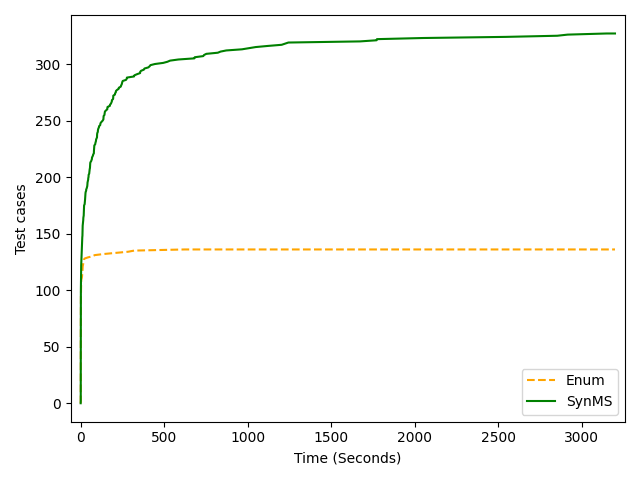
\includegraphics[width=\textwidth]{fig/normal-sub-f.png}
        \caption{Cumulative solved formula cases}
    \end{subfigure}
    \begin{subfigure}[b]{0.49\textwidth}
        \centering
        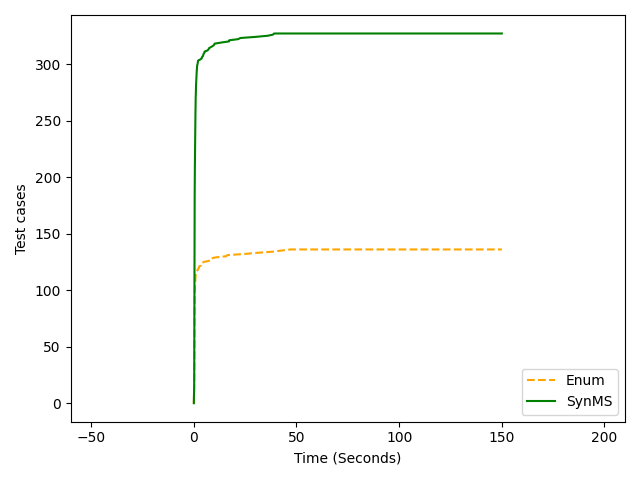
\includegraphics[width=\textwidth]{fig/normal-sub-s.png}
        \caption{Cumulative solved strategy cases}
    \end{subfigure}
    \caption{Cumulative solved test cases over time for Subtraction game under normal rule}
    \label{fig:normal-sub-line}
\end{figure}

\textbf{Comparison on Nim game.}
Table~\ref{tab:normal-nim-winFormulas}~presents the results for synthesizing winning formulas in the Nim game under the normal rule.
Out of $302$ test cases, Enum solves $62$ formula cases, while SynMS solves $95$, with success rates of $20.5\%$ and $31.5\%$, respectively.
Thus SynMS solves $33$ more formula cases than Enum.
The average formula synthesis time is $9.77$ seconds for Enum and $5.70$ seconds for SynMS.
Table~\ref{tab:normal-nim-winStrategies}~summarizes the corresponding results for synthesizing winning strategies.
Enum solves $59$ strategy cases, whereas SynMS solves $86$ strategy cases.
This gives SynMS an advantage of $27$ strategy cases in this benchmark group.
The average strategy synthesis time is $44.60$ seconds for Enum and $63.38$ seconds for SynMS.
In terms of solution size, Enum produces smaller formulas and strategies on average, with average sizes $5.77$ and $28.63$, while SynMS has average sizes $71.34$ and $481.79$.
Figure~\ref{fig:normal-nim-line}~shows the cumulative number of solved test cases over time using the same solved-case filtering as the tables.

\begin{table*}[h!]
	%字体大小和行距
	\scriptsize
	%列距
	\setlength{\tabcolsep}{1pt}
	\centering
	\resizebox{\textwidth}{!}{%
	\renewcommand{\arraystretch}{1.12}%
	\begin{tabular}{|c|c|c|c|c|c|c|c|}
		\hline
		\multirow{3}{*}{Category} & \multirow{3}*{\tabincell{c}{Test \\ cases}} & \multicolumn{6}{c|}{Formula}  \\ \cline{3-8} &  & \multicolumn{2}{c|}{Solved} & \multicolumn{2}{c|}{Time} & \multicolumn{2}{c|}{Size} \\ \cline{3-8} & & \multicolumn{1}{c|}{Enum} & \multicolumn{1}{c|}{SynMS} & \multicolumn{1}{c|}{Enum} & \multicolumn{1}{c|}{SynMS} & \multicolumn{1}{c|}{Enum} & SynMS \\ \hline
		Nim & 7 & 1(0) & \textbf{2}(1) & \textbf{1.13}(1.13) & 3.66(\textbf{1.12}) & \textbf{4.00}(4.00) & 23.50(\textbf{3.00}) \\ \hline
		Monotonic Nim & 7 & \textbf{7}(0) & \textbf{7}(0) & \textbf{0.94}(\textbf{0.94}) & 1.28(1.28) & 4.86(4.86) & \textbf{3.86}(\textbf{3.86}) \\ \hline
		Empty and Transfer & 7 & \textbf{2}(1) & 1(0) & \textbf{2.83}(4.50) & 2.98(\textbf{2.98}) & \textbf{7.50}(\textbf{7.00}) & 18.00(18.00) \\ \hline
		Empty All But One & 6 & \textbf{6}(0) & \textbf{6}(0) & 24.40(24.40) & \textbf{4.64}(\textbf{4.64}) & \textbf{5.33}(\textbf{5.33}) & 32.00(32.00) \\ \hline
		Empty and Redistribute & 6 & 1(1) & \textbf{2}(2) & 36.61(-) & \textbf{2.65}(-) & \textbf{13.00}(-) & 178.00(-) \\ \hline
		Entropy Reduction Game & 7 & \textbf{1}(0) & \textbf{1}(0) & \textbf{12.63}(\textbf{12.63}) & 19.53(19.53) & \textbf{8.00}(\textbf{8.00}) & 12.00(12.00) \\ \hline
		Min Game & 6 & 1(0) & \textbf{3}(2) & \textbf{3.10}(3.10) & 8.95(\textbf{3.00}) & \textbf{6.00}(6.00) & 117.67(\textbf{5.00}) \\ \hline
		$l$-Slow Nim & 180 & 9(1) & \textbf{11}(3) & \textbf{1.42}(\textbf{1.40}) & 7.19(6.46) & \textbf{4.89}(\textbf{4.88}) & 135.09(59.50) \\ \hline
		Sharing Nim & 7 & 4(0) & \textbf{6}(2) & \textbf{4.78}(4.78) & 6.31(\textbf{3.83}) & \textbf{5.00}(\textbf{5.00}) & 10.83(5.25) \\ \hline
		Small Nim & 7 & \textbf{7}(0) & \textbf{7}(0) & 18.29(18.29) & \textbf{1.70}(\textbf{1.70}) & \textbf{7.29}(\textbf{7.29}) & 11.86(11.86) \\ \hline
		Greedy Nim & 7 & 2(0) & \textbf{7}(5) & 6.92(6.92) & \textbf{5.47}(\textbf{1.09}) & \textbf{8.50}(\textbf{8.50}) & 159.86(19.50) \\ \hline
		Odd-or-Even Nim & 7 & 2(0) & \textbf{6}(4) & 3.88(3.88) & \textbf{3.28}(\textbf{1.34}) & \textbf{7.00}(\textbf{7.00}) & 230.83(21.00) \\ \hline
		Modular Nim & 5 & 1(0) & \textbf{2}(1) & \textbf{1.12}(\textbf{1.12}) & 1.94(1.32) & \textbf{4.00}(\textbf{4.00}) & 30.00(12.00) \\ \hline
		Pointed Nim & 7 & 1(0) & \textbf{7}(6) & 23.07(\textbf{23.07}) & \textbf{9.84}(24.00) & \textbf{4.00}(\textbf{4.00}) & 49.29(\textbf{4.00}) \\ \hline
		End Nim & 7 & 1(0) & \textbf{7}(6) & \textbf{1.08}(1.08) & 2.48(\textbf{0.86}) & \textbf{4.00}(\textbf{4.00}) & 107.71(\textbf{4.00}) \\ \hline
		Loop End Nim & 7 & 2(0) & \textbf{7}(5) & 78.32(78.32) & \textbf{13.02}(\textbf{6.46}) & \textbf{9.50}(\textbf{9.50}) & 51.86(30.00) \\ \hline
		Staircase Nim & 7 & \textbf{7}(0) & \textbf{7}(0) & \textbf{1.79}(\textbf{1.79}) & 2.52(2.52) & 3.71(3.71) & \textbf{2.86}(\textbf{2.86}) \\ \hline
		Circular Nim & 15 & \textbf{7}(1) & 6(0) & \textbf{2.52}(\textbf{1.65}) & 9.58(9.58) & \textbf{6.14}(\textbf{5.67}) & 15.33(15.33) \\ \hline
		Total & 302 & 62(4) & \textbf{95}(37) & 9.77(9.63) & \textbf{5.70}(\textbf{4.51}) & \textbf{5.77}(\textbf{5.57}) & 71.34(19.14) \\ \hline
	\end{tabular}%
	}
	\caption{Results of synthesizing winning formulas for Nim games under normal rule}
	\label{tab:normal-nim-winFormulas}
\end{table*}

\begin{table*}[h!]
	%字体大小和行距
	\scriptsize
	%列距
	\setlength{\tabcolsep}{1pt}
	\centering
	\resizebox{\textwidth}{!}{%
	\renewcommand{\arraystretch}{1.12}%
	\begin{tabular}{|c|c|c|c|c|c|c|c|}
		\hline
		\multirow{3}{*}{Category} & \multirow{3}*{\tabincell{c}{Test \\ cases}} & \multicolumn{6}{c|}{Strategy}  \\ \cline{3-8} &  & \multicolumn{2}{c|}{Solved} & \multicolumn{2}{c|}{Time} & \multicolumn{2}{c|}{Size} \\ \cline{3-8} & & \multicolumn{1}{c|}{Enum} & \multicolumn{1}{c|}{SynMS} & \multicolumn{1}{c|}{Enum} & \multicolumn{1}{c|}{SynMS} & \multicolumn{1}{c|}{Enum} & SynMS \\ \hline
		Nim & 7 & 1(0) & \textbf{2}(1) & 1.12(1.12) & \textbf{0.17}(\textbf{0.04}) & \textbf{12.00}(\textbf{12.00}) & 54.00(\textbf{12.00}) \\ \hline
		Monotonic Nim & 7 & \textbf{7}(0) & \textbf{7}(0) & 1.16(1.16) & \textbf{0.09}(\textbf{0.09}) & 28.86(28.86) & \textbf{22.86}(\textbf{22.86}) \\ \hline
		Empty and Transfer & 7 & \textbf{2}(1) & 1(0) & \textbf{0.78}(\textbf{0.71}) & 9.61(9.61) & 18.00(14.00) & \textbf{12.00}(\textbf{12.00}) \\ \hline
		Empty All But One & 6 & \textbf{6}(0) & \textbf{6}(0) & \textbf{7.47}(\textbf{7.47}) & 16.22(16.22) & \textbf{5.33}(\textbf{5.33}) & \textbf{5.33}(\textbf{5.33}) \\ \hline
		Empty and Redistribute & 6 & 0(0) & \textbf{1}(1) & -(-) & 24.35(-) & -(-) & 9.00(-) \\ \hline
		Entropy Reduction Game & 7 & 0(0) & \textbf{1}(1) & -(-) & 4.08(-) & -(-) & 112.00(-) \\ \hline
		Min Game & 6 & 1(0) & \textbf{3}(2) & \textbf{0.46}(\textbf{0.46}) & 45.96(2.32) & \textbf{11.00}(\textbf{11.00}) & 3216.33(113.00) \\ \hline
		$l$-Slow Nim & 180 & 9(1) & \textbf{11}(3) & \textbf{0.49}(\textbf{0.41}) & 38.37(51.97) & \textbf{30.89}(\textbf{26.75}) & 821.09(311.25) \\ \hline
		Sharing Nim & 7 & 3(0) & \textbf{6}(3) & \textbf{0.44}(\textbf{0.44}) & 35.95(22.21) & \textbf{22.33}(\textbf{22.33}) & 1234.50(627.33) \\ \hline
		Small Nim & 7 & \textbf{7}(0) & \textbf{7}(0) & 2.72(2.72) & \textbf{1.25}(\textbf{1.25}) & 72.57(72.57) & \textbf{30.86}(\textbf{30.86}) \\ \hline
		Greedy Nim & 7 & 2(0) & \textbf{5}(3) & \textbf{1.49}(\textbf{1.49}) & 282.73(21.04) & \textbf{49.50}(\textbf{49.50}) & 1101.40(177.50) \\ \hline
		Odd-or-Even Nim & 7 & 2(0) & \textbf{6}(4) & \textbf{0.89}(\textbf{0.89}) & 259.60(19.98) & \textbf{16.50}(\textbf{16.50}) & 859.83(66.00) \\ \hline
		Modular Nim & 5 & 1(0) & \textbf{2}(1) & \textbf{0.51}(\textbf{0.51}) & 2.15(3.63) & \textbf{14.00}(\textbf{14.00}) & 55.00(32.00) \\ \hline
		Pointed Nim & 7 & 1(0) & \textbf{7}(6) & 0.74(0.74) & \textbf{0.53}(\textbf{0.05}) & \textbf{8.00}(\textbf{8.00}) & 11.43(\textbf{8.00}) \\ \hline
		End Nim & 7 & 1(0) & \textbf{4}(3) & \textbf{1.08}(1.08) & 147.56(\textbf{0.04}) & \textbf{8.00}(\textbf{8.00}) & 336.75(\textbf{8.00}) \\ \hline
		Loop End Nim & 7 & 2(0) & \textbf{7}(5) & \textbf{1.24}(\textbf{1.24}) & 109.37(40.79) & \textbf{25.00}(\textbf{25.00}) & 335.86(467.50) \\ \hline
		Staircase Nim & 7 & \textbf{7}(0) & \textbf{7}(0) & 2.06(2.06) & \textbf{0.07}(\textbf{0.07}) & 23.71(23.71) & \textbf{17.43}(\textbf{17.43}) \\ \hline
		Circular Nim & 15 & \textbf{7}(4) & 3(0) & 360.97(\textbf{0.94}) & \textbf{64.87}(64.87) & 23.57(\textbf{7.00}) & \textbf{7.00}(\textbf{7.00}) \\ \hline
		Total & 302 & 59(6) & \textbf{86}(33) & \textbf{44.60}(\textbf{1.99}) & 63.38(18.18) & \textbf{28.63}(\textbf{27.53}) & 481.79(123.21) \\ \hline
	\end{tabular}%
	}
	\caption{Results of synthesizing winning strategies for Nim games under normal rule}
	\label{tab:normal-nim-winStrategies}
\end{table*}

\begin{figure}[h!]
    \centering
    \begin{subfigure}[b]{0.49\textwidth}
        \centering
        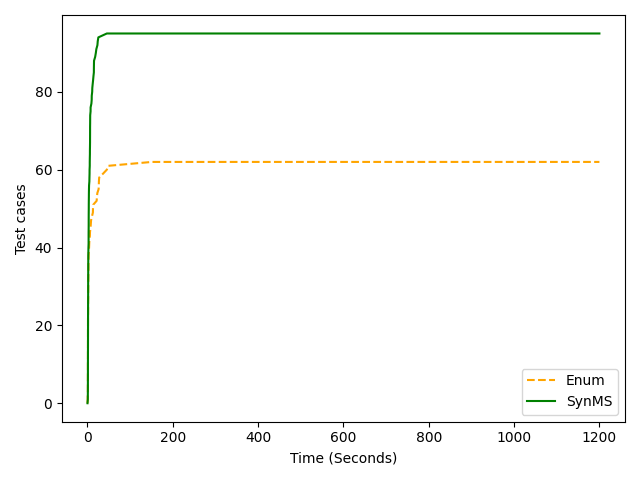
\includegraphics[width=\textwidth]{fig/normal-nim-f.png}
        \caption{Cumulative solved formula cases}
    \end{subfigure}
    \begin{subfigure}[b]{0.49\textwidth}
        \centering
        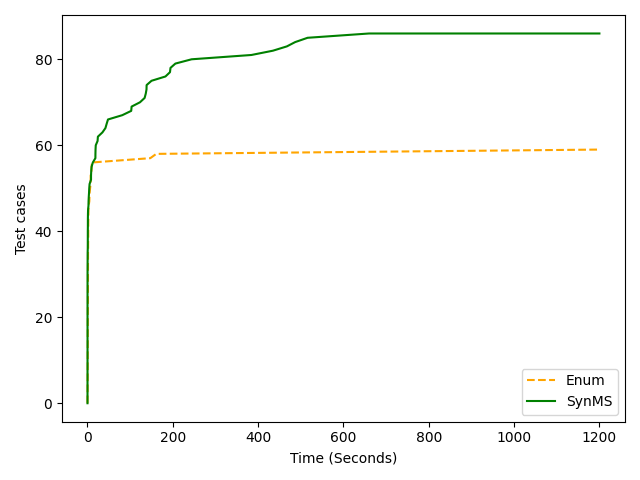
\includegraphics[width=\textwidth]{fig/normal-nim-s.png}
        \caption{Cumulative solved strategy cases}
    \end{subfigure}
    \caption{Cumulative solved test cases over time for Nim game under normal rule}
    \label{fig:normal-nim-line}
\end{figure}

\textbf{Comparison on Welter game.}
Table~\ref{tab:normal-welter-winFormulas}~presents the results for synthesizing winning formulas in the Welter game under the normal rule.
Out of $7$ test cases, Enum solves $4$ formula cases, while SynMS solves $5$, with success rates of $57.1\%$ and $71.4\%$, respectively.
Thus SynMS solves $1$ more formula cases than Enum.
The average formula synthesis time is $62.06$ seconds for Enum and $3.50$ seconds for SynMS.
Table~\ref{tab:normal-welter-winStrategies}~summarizes the corresponding results for synthesizing winning strategies.
Enum solves $4$ strategy cases, whereas SynMS solves $5$ strategy cases.
This gives SynMS an advantage of $1$ strategy cases in this benchmark group.
The average strategy synthesis time is $1.12$ seconds for Enum and $0.55$ seconds for SynMS.
In terms of solution size, Enum produces smaller formulas and strategies on average, with average sizes $8.00$ and $39.00$, while SynMS has average sizes $74.40$ and $399.20$.
Figure~\ref{fig:normal-welter-line}~shows the cumulative number of solved test cases over time using the same solved-case filtering as the tables.

\begin{table*}[h!]
	%字体大小和行距
	\footnotesize
	%列距
	\setlength{\tabcolsep}{3pt}
	\centering
	\resizebox{\textwidth}{!}{%
	\renewcommand{\arraystretch}{1.12}%
	\begin{tabular}{|c|c|c|c|c|c|c|c|}
		\hline
		\multirow{3}{*}{Category} & \multirow{3}*{\tabincell{c}{Test \\ cases}} & \multicolumn{6}{c|}{Formula}  \\ \cline{3-8} &  & \multicolumn{2}{c|}{Solved} & \multicolumn{2}{c|}{Time} & \multicolumn{2}{c|}{Size} \\ \cline{3-8} & & \multicolumn{1}{c|}{Enum} & \multicolumn{1}{c|}{SynMS} & \multicolumn{1}{c|}{Enum} & \multicolumn{1}{c|}{SynMS} & \multicolumn{1}{c|}{Enum} & SynMS \\ \hline
		Welter & 1 & \textbf{1}(0) & \textbf{1}(0) & 123.22(123.22) & \textbf{3.00}(\textbf{3.00}) & \textbf{12.00}(\textbf{12.00}) & 36.00(36.00) \\ \hline
		$l$-Welter & 5 & 2(0) & \textbf{3}(1) & \textbf{1.09}(\textbf{1.09}) & 4.35(2.53) & \textbf{4.00}(\textbf{4.00}) & 100.00(42.00) \\ \hline
		Max-Welter & 1 & \textbf{1}(0) & \textbf{1}(0) & 122.86(122.86) & \textbf{1.46}(\textbf{1.46}) & \textbf{12.00}(\textbf{12.00}) & 36.00(36.00) \\ \hline
		Total & 7 & 4(0) & \textbf{5}(1) & 62.06(62.06) & \textbf{3.50}(\textbf{2.38}) & \textbf{8.00}(\textbf{8.00}) & 74.40(39.00) \\ \hline
	\end{tabular}%
	}
	\caption{Results of synthesizing winning formulas for Welter games under normal rule}
	\label{tab:normal-welter-winFormulas}
\end{table*}

\begin{table*}[h!]
	%字体大小和行距
	\footnotesize
	%列距
	\setlength{\tabcolsep}{3pt}
	\centering
	\resizebox{\textwidth}{!}{%
	\renewcommand{\arraystretch}{1.12}%
	\begin{tabular}{|c|c|c|c|c|c|c|c|}
		\hline
		\multirow{3}{*}{Category} & \multirow{3}*{\tabincell{c}{Test \\ cases}} & \multicolumn{6}{c|}{Strategy}  \\ \cline{3-8} &  & \multicolumn{2}{c|}{Solved} & \multicolumn{2}{c|}{Time} & \multicolumn{2}{c|}{Size} \\ \cline{3-8} & & \multicolumn{1}{c|}{Enum} & \multicolumn{1}{c|}{SynMS} & \multicolumn{1}{c|}{Enum} & \multicolumn{1}{c|}{SynMS} & \multicolumn{1}{c|}{Enum} & SynMS \\ \hline
		Welter & 1 & \textbf{1}(0) & \textbf{1}(0) & 1.75(1.75) & \textbf{0.23}(\textbf{0.23}) & 44.00(44.00) & \textbf{38.00}(\textbf{38.00}) \\ \hline
		$l$-Welter & 5 & 2(0) & \textbf{3}(1) & \textbf{0.39}(0.39) & 0.78(\textbf{0.30}) & \textbf{30.00}(\textbf{30.00}) & 637.33(197.00) \\ \hline
		Max-Welter & 1 & \textbf{1}(0) & \textbf{1}(0) & 1.96(1.96) & \textbf{0.17}(\textbf{0.17}) & 52.00(52.00) & \textbf{46.00}(\textbf{46.00}) \\ \hline
		Total & 7 & 4(0) & \textbf{5}(1) & 1.12(1.12) & \textbf{0.55}(\textbf{0.25}) & \textbf{39.00}(\textbf{39.00}) & 399.20(119.50) \\ \hline
	\end{tabular}%
	}
	\caption{Results of synthesizing winning strategies for Welter games under normal rule}
	\label{tab:normal-welter-winStrategies}
\end{table*}

\begin{figure}[h!]
    \centering
    \begin{subfigure}[b]{0.49\textwidth}
        \centering
        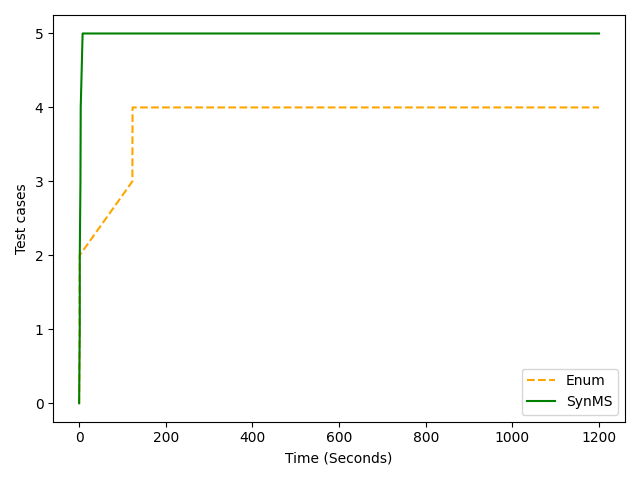
\includegraphics[width=\textwidth]{fig/normal-welter-f.png}
        \caption{Cumulative solved formula cases}
    \end{subfigure}
    \begin{subfigure}[b]{0.49\textwidth}
        \centering
        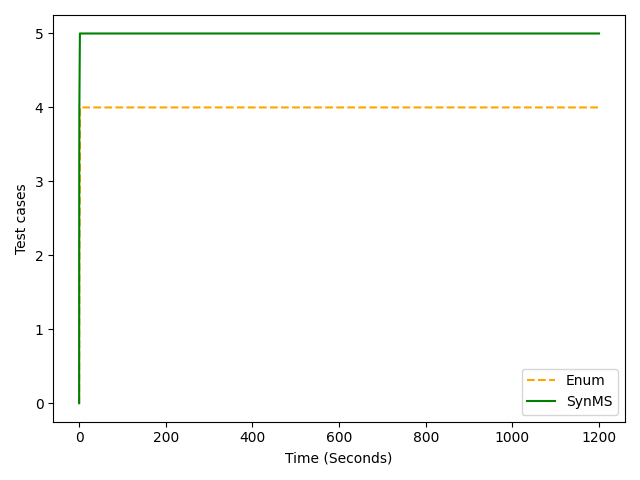
\includegraphics[width=\textwidth]{fig/normal-welter-s.png}
        \caption{Cumulative solved strategy cases}
    \end{subfigure}
    \caption{Cumulative solved test cases over time for Welter game under normal rule}
    \label{fig:normal-welter-line}
\end{figure}

\textbf{Comparison on Wythoff game.}
Table~\ref{tab:normal-wythoff-winFormulas}~presents the results for synthesizing winning formulas in the Wythoff game under the normal rule.
Out of $2924$ test cases, Enum solves $1863$ formula cases, while SynMS solves $2679$, with success rates of $63.7\%$ and $91.6\%$, respectively.
Thus SynMS solves $816$ more formula cases than Enum.
The average formula synthesis time is $24.24$ seconds for Enum and $15.29$ seconds for SynMS.
Table~\ref{tab:normal-wythoff-winStrategies}~summarizes the corresponding results for synthesizing winning strategies.
Enum solves $1815$ strategy cases, whereas SynMS solves $2200$ strategy cases.
This gives SynMS an advantage of $385$ strategy cases in this benchmark group.
The average strategy synthesis time is $2.08$ seconds for Enum and $246.62$ seconds for SynMS.
In terms of solution size, Enum produces smaller formulas and strategies on average, with average sizes $5.57$ and $37.95$, while SynMS has average sizes $44.80$ and $380.59$.
Figure~\ref{fig:normal-wythoff-line}~shows the cumulative number of solved test cases over time using the same solved-case filtering as the tables.

\begin{table*}[h!]
	%字体大小和行距
	\tiny
	%列距
	\setlength{\tabcolsep}{0.8pt}
	\centering
	\resizebox{\textwidth}{!}{%
	\renewcommand{\arraystretch}{1.12}%
	\begin{tabular}{|c|c|c|c|c|c|c|c|}
		\hline
		\multirow{3}{*}{Category} & \multirow{3}*{\tabincell{c}{Test \\ cases}} & \multicolumn{6}{c|}{Formula}  \\ \cline{3-8} &  & \multicolumn{2}{c|}{Solved} & \multicolumn{2}{c|}{Time} & \multicolumn{2}{c|}{Size} \\ \cline{3-8} & & \multicolumn{1}{c|}{Enum} & \multicolumn{1}{c|}{SynMS} & \multicolumn{1}{c|}{Enum} & \multicolumn{1}{c|}{SynMS} & \multicolumn{1}{c|}{Enum} & SynMS \\ \hline
		Wythoff & 21 & 13(0) & \textbf{19}(6) & 11.18(11.18) & \textbf{2.44}(\textbf{2.56}) & \textbf{5.77}(\textbf{5.77}) & 49.95(17.54) \\ \hline
		$l$-Wythoff & 140 & 93(1) & \textbf{120}(28) & \textbf{25.64}(25.81) & 40.09(\textbf{21.19}) & \textbf{6.45}(\textbf{6.43}) & 63.65(41.23) \\ \hline
		Monotonic $l$-Diet Wythoff & 105 & 81(1) & \textbf{103}(23) & 13.69(13.81) & \textbf{6.39}(\textbf{3.14}) & \textbf{5.49}(\textbf{5.49}) & 78.92(40.67) \\ \hline
		Wythoff with subtraction set $S$ & 315 & 177(0) & \textbf{287}(110) & 22.86(22.86) & \textbf{2.84}(\textbf{2.49}) & \textbf{5.76}(\textbf{5.76}) & 55.32(20.49) \\ \hline
		Wythoff with a function $f$ & 168 & 118(0) & \textbf{154}(36) & 16.44(16.44) & \textbf{4.71}(\textbf{2.97}) & \textbf{5.59}(\textbf{5.59}) & 47.68(29.14) \\ \hline
		1st($l_1$,$l_2$)\-restricted Wythoff & 315 & 119(0) & \textbf{285}(166) & 25.64(25.64) & \textbf{2.26}(\textbf{2.05}) & \textbf{6.03}(\textbf{6.03}) & 57.56(21.94) \\ \hline
		2nd($l_1$,$l_2$)\-restricted Wythoff & 600 & 543(0) & \textbf{600}(57) & 29.32(29.32) & \textbf{2.12}(\textbf{2.05}) & \textbf{4.83}(\textbf{4.83}) & 24.04(17.27) \\ \hline
		3rd($l_1$,$l_2$)\-restricted Wythoff & 700 & 392(0) & \textbf{578}(186) & \textbf{29.69}(29.69) & 50.54(\textbf{9.08}) & \textbf{6.51}(\textbf{6.51}) & 50.73(31.17) \\ \hline
		4th($l_1$,$l_2$)\-restricted Wythoff & 560 & 327(0) & \textbf{533}(206) & 15.06(15.06) & \textbf{5.21}(\textbf{2.29}) & \textbf{5.18}(\textbf{5.18}) & 37.42(13.22) \\ \hline
		Total & 2924 & 1863(2) & \textbf{2679}(818) & 24.24(24.26) & \textbf{15.29}(\textbf{4.67}) & \textbf{5.57}(\textbf{5.57}) & 44.80(23.03) \\ \hline
	\end{tabular}%
	}
	\caption{Results of synthesizing winning formulas for Wythoff games under normal rule}
	\label{tab:normal-wythoff-winFormulas}
\end{table*}

\begin{table*}[h!]
	%字体大小和行距
	\tiny
	%列距
	\setlength{\tabcolsep}{0.8pt}
	\centering
	\resizebox{\textwidth}{!}{%
	\renewcommand{\arraystretch}{1.12}%
	\begin{tabular}{|c|c|c|c|c|c|c|c|}
		\hline
		\multirow{3}{*}{Category} & \multirow{3}*{\tabincell{c}{Test \\ cases}} & \multicolumn{6}{c|}{Strategy}  \\ \cline{3-8} &  & \multicolumn{2}{c|}{Solved} & \multicolumn{2}{c|}{Time} & \multicolumn{2}{c|}{Size} \\ \cline{3-8} & & \multicolumn{1}{c|}{Enum} & \multicolumn{1}{c|}{SynMS} & \multicolumn{1}{c|}{Enum} & \multicolumn{1}{c|}{SynMS} & \multicolumn{1}{c|}{Enum} & SynMS \\ \hline
		Wythoff & 21 & \textbf{13}(1) & 12(0) & \textbf{1.22}(\textbf{1.05}) & 6.48(6.48) & \textbf{36.15}(\textbf{27.00}) & 55.75(55.75) \\ \hline
		$l$-Wythoff & 140 & \textbf{93}(24) & 73(4) & \textbf{2.77}(\textbf{2.44}) & 402.79(376.59) & \textbf{56.42}(\textbf{45.86}) & 434.71(298.39) \\ \hline
		Monotonic $l$-Diet Wythoff & 105 & 81(1) & \textbf{103}(23) & \textbf{0.47}(0.46) & 0.64(\textbf{0.39}) & \textbf{27.43}(\textbf{27.05}) & 477.36(245.06) \\ \hline
		Wythoff with subtraction set $S$ & 315 & 177(0) & \textbf{253}(76) & \textbf{1.50}(\textbf{1.50}) & 15.14(6.17) & \textbf{31.39}(\textbf{31.39}) & 437.05(159.77) \\ \hline
		Wythoff with a function $f$ & 168 & \textbf{118}(19) & 110(11) & \textbf{1.92}(\textbf{1.79}) & 178.94(150.36) & \textbf{35.04}(\textbf{29.24}) & 216.99(170.13) \\ \hline
		1st($l_1$,$l_2$)\-restricted Wythoff & 315 & 119(0) & \textbf{257}(138) & \textbf{1.76}(\textbf{1.76}) & 11.06(5.66) & \textbf{31.39}(\textbf{31.39}) & 457.32(207.94) \\ \hline
		2nd($l_1$,$l_2$)\-restricted Wythoff & 600 & 543(15) & \textbf{577}(49) & \textbf{1.70}(\textbf{1.66}) & 542.39(488.22) & \textbf{34.10}(\textbf{32.30}) & 400.03(214.77) \\ \hline
		3rd($l_1$,$l_2$)\-restricted Wythoff & 700 & \textbf{392}(54) & 350(12) & \textbf{3.47}(\textbf{3.06}) & 429.75(408.42) & \textbf{57.16}(\textbf{50.30}) & 313.33(266.46) \\ \hline
		4th($l_1$,$l_2$)\-restricted Wythoff & 560 & 279(0) & \textbf{465}(186) & \textbf{1.72}(\textbf{1.72}) & 50.08(30.76) & \textbf{23.65}(\textbf{23.65}) & 351.11(230.91) \\ \hline
		Total & 2924 & 1815(114) & \textbf{2200}(499) & \textbf{2.08}(\textbf{1.92}) & 246.62(262.88) & \textbf{37.95}(\textbf{34.39}) & 380.59(222.58) \\ \hline
	\end{tabular}%
	}
	\caption{Results of synthesizing winning strategies for Wythoff games under normal rule}
	\label{tab:normal-wythoff-winStrategies}
\end{table*}

\begin{figure}[h!]
    \centering
    \begin{subfigure}[b]{0.49\textwidth}
        \centering
        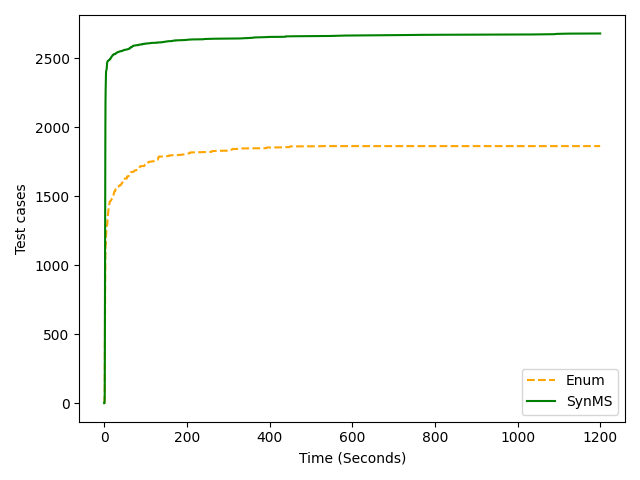
\includegraphics[width=\textwidth]{fig/normal-wythoff-f.png}
        \caption{Cumulative solved formula cases}
    \end{subfigure}
    \begin{subfigure}[b]{0.49\textwidth}
        \centering
        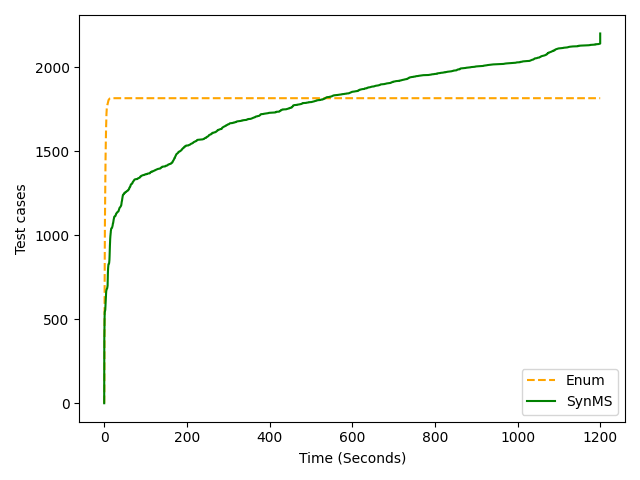
\includegraphics[width=\textwidth]{fig/normal-wythoff-s.png}
        \caption{Cumulative solved strategy cases}
    \end{subfigure}
    \caption{Cumulative solved test cases over time for Wythoff game under normal rule}
    \label{fig:normal-wythoff-line}
\end{figure}

\textbf{Comparison on Chomp game.}
Table~\ref{tab:normal-chomp-winFormulas}~presents the results for synthesizing winning formulas in the Chomp game under the normal rule.
Out of $8$ test cases, Enum solves $2$ formula cases, while SynMS solves $3$, with success rates of $25.0\%$ and $37.5\%$, respectively.
Thus SynMS solves $1$ more formula cases than Enum.
The average formula synthesis time is $1.40$ seconds for Enum and $4.46$ seconds for SynMS.
Table~\ref{tab:normal-chomp-winStrategies}~summarizes the corresponding results for synthesizing winning strategies.
Enum solves $2$ strategy cases, whereas SynMS solves $2$ strategy cases.
Both approaches solve $2$ strategy cases in this benchmark group.
The average strategy synthesis time is $2.26$ seconds for Enum and $5.26$ seconds for SynMS.
In terms of solution size, Enum produces smaller formulas and strategies on average, with average sizes $4.00$ and $9.50$, while SynMS has average sizes $42.00$ and $10.00$.
Figure~\ref{fig:normal-chomp-line}~shows the cumulative number of solved test cases over time using the same solved-case filtering as the tables.

\begin{table*}[h!]
	%字体大小和行距
	\footnotesize
	%列距
	\setlength{\tabcolsep}{3pt}
	\centering
	\resizebox{\textwidth}{!}{%
	\renewcommand{\arraystretch}{1.12}%
	\begin{tabular}{|c|c|c|c|c|c|c|c|}
		\hline
		\multirow{3}{*}{Category} & \multirow{3}*{\tabincell{c}{Test \\ cases}} & \multicolumn{6}{c|}{Formula}  \\ \cline{3-8} &  & \multicolumn{2}{c|}{Solved} & \multicolumn{2}{c|}{Time} & \multicolumn{2}{c|}{Size} \\ \cline{3-8} & & \multicolumn{1}{c|}{Enum} & \multicolumn{1}{c|}{SynMS} & \multicolumn{1}{c|}{Enum} & \multicolumn{1}{c|}{SynMS} & \multicolumn{1}{c|}{Enum} & SynMS \\ \hline
		Chomp & 7 & 1(0) & \textbf{2}(1) & \textbf{1.21}(\textbf{1.21}) & 5.93(1.64) & \textbf{4.00}(4.00) & 61.50(\textbf{3.00}) \\ \hline
		L-shaped Chomp & 1 & \textbf{1}(0) & \textbf{1}(0) & 1.59(1.59) & \textbf{1.53}(\textbf{1.53}) & 4.00(4.00) & \textbf{3.00}(\textbf{3.00}) \\ \hline
		Total & 8 & 2(0) & \textbf{3}(1) & \textbf{1.40}(\textbf{1.40}) & 4.46(1.59) & \textbf{4.00}(4.00) & 42.00(\textbf{3.00}) \\ \hline
	\end{tabular}%
	}
	\caption{Results of synthesizing winning formulas for Chomp games under normal rule}
	\label{tab:normal-chomp-winFormulas}
\end{table*}

\begin{table*}[h!]
	%字体大小和行距
	\footnotesize
	%列距
	\setlength{\tabcolsep}{3pt}
	\centering
	\resizebox{\textwidth}{!}{%
	\renewcommand{\arraystretch}{1.12}%
	\begin{tabular}{|c|c|c|c|c|c|c|c|}
		\hline
		\multirow{3}{*}{Category} & \multirow{3}*{\tabincell{c}{Test \\ cases}} & \multicolumn{6}{c|}{Strategy}  \\ \cline{3-8} &  & \multicolumn{2}{c|}{Solved} & \multicolumn{2}{c|}{Time} & \multicolumn{2}{c|}{Size} \\ \cline{3-8} & & \multicolumn{1}{c|}{Enum} & \multicolumn{1}{c|}{SynMS} & \multicolumn{1}{c|}{Enum} & \multicolumn{1}{c|}{SynMS} & \multicolumn{1}{c|}{Enum} & SynMS \\ \hline
		Chomp & 7 & \textbf{1}(0) & \textbf{1}(0) & \textbf{3.57}(\textbf{3.57}) & 10.47(10.47) & \textbf{9.00}(\textbf{9.00}) & 10.00(10.00) \\ \hline
		L-shaped Chomp & 1 & \textbf{1}(0) & \textbf{1}(0) & 0.96(0.96) & \textbf{0.04}(\textbf{0.04}) & \textbf{10.00}(\textbf{10.00}) & \textbf{10.00}(\textbf{10.00}) \\ \hline
		Total & 8 & \textbf{2}(0) & \textbf{2}(0) & \textbf{2.26}(\textbf{2.26}) & 5.26(5.26) & \textbf{9.50}(\textbf{9.50}) & 10.00(10.00) \\ \hline
	\end{tabular}%
	}
	\caption{Results of synthesizing winning strategies for Chomp games under normal rule}
	\label{tab:normal-chomp-winStrategies}
\end{table*}

\begin{figure}[h!]
    \centering
    \begin{subfigure}[b]{0.49\textwidth}
        \centering
        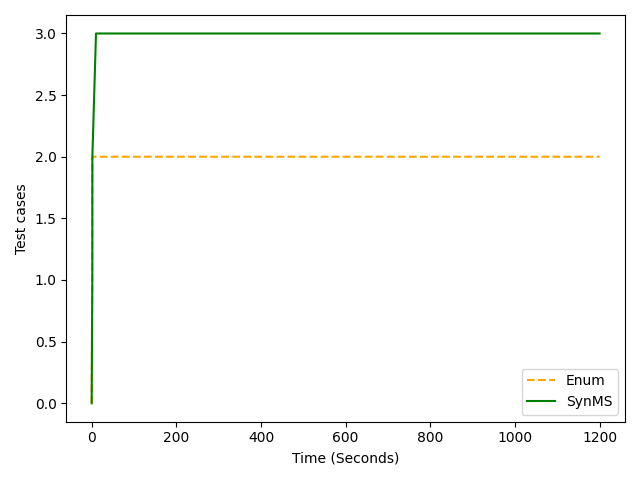
\includegraphics[width=\textwidth]{fig/normal-chomp-f.png}
        \caption{Cumulative solved formula cases}
    \end{subfigure}
    \begin{subfigure}[b]{0.49\textwidth}
        \centering
        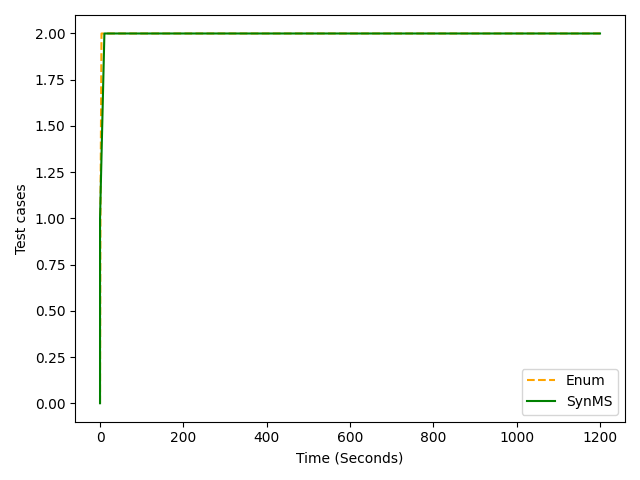
\includegraphics[width=\textwidth]{fig/normal-chomp-s.png}
        \caption{Cumulative solved strategy cases}
    \end{subfigure}
    \caption{Cumulative solved test cases over time for Chomp game under normal rule}
    \label{fig:normal-chomp-line}
\end{figure}

\subsubsection{Experimental Results under mis\`{e}re rule}

\textbf{Comparison on Subtraction game.}
Table~\ref{tab:misere-sub-winFormulas}~presents the results for synthesizing winning formulas in the Subtraction game under the mis\`{e}re rule.
Out of $479$ test cases, Enum solves $178$ formula cases, while SynMS solves $346$, with success rates of $37.2\%$ and $72.2\%$, respectively.
Thus SynMS solves $168$ more formula cases than Enum.
The average formula synthesis time is $16.17$ seconds for Enum and $297.19$ seconds for SynMS.
Table~\ref{tab:misere-sub-winStrategies}~summarizes the corresponding results for synthesizing winning strategies.
Enum solves $176$ strategy cases, whereas SynMS solves $346$ strategy cases.
This gives SynMS an advantage of $170$ strategy cases in this benchmark group.
The average strategy synthesis time is $2.17$ seconds for Enum and $4.67$ seconds for SynMS.
In terms of solution size, Enum produces smaller formulas and strategies on average, with average sizes $9.13$ and $55.60$, while SynMS has average sizes $16.18$ and $56.24$.
Figure~\ref{fig:misere-sub-line}~shows the cumulative number of solved test cases over time using the same per-case data as the tables.

\begin{table*}[h!]
	%字体大小和行距
	\footnotesize
	%列距
	\setlength{\tabcolsep}{2pt}
	\centering
	\resizebox{\textwidth}{!}{%
	\renewcommand{\arraystretch}{1.12}%
	\begin{tabular}{|c|c|c|c|c|c|c|c|}
		\hline
		\multirow{3}{*}{Category} & \multirow{3}*{\tabincell{c}{Test \\ cases}} & \multicolumn{6}{c|}{Formula}  \\ \cline{3-8} &  & \multicolumn{2}{c|}{Solved} & \multicolumn{2}{c|}{Time} & \multicolumn{2}{c|}{Size} \\ \cline{3-8} & & \multicolumn{1}{c|}{Enum} & \multicolumn{1}{c|}{SynMS} & \multicolumn{1}{c|}{Enum} & \multicolumn{1}{c|}{SynMS} & \multicolumn{1}{c|}{Enum} & SynMS \\ \hline
		Take-away & 30 & \textbf{30}(0) & \textbf{30}(0) & \textbf{5.13}(\textbf{5.13}) & 19.62(19.62) & \textbf{3.00}(\textbf{3.00}) & \textbf{3.00}(\textbf{3.00}) \\ \hline
		Subtraction & 385 & 96(27) & \textbf{263}(194) & \textbf{27.98}(\textbf{29.30}) & 382.85(292.75) & \textbf{14.38}(11.52) & 19.32(\textbf{11.43}) \\ \hline
		$S,D$-Mark & 64 & 52(0) & \textbf{53}(1) & \textbf{0.74}(\textbf{0.74}) & 29.25(1.06) & \textbf{3.00}(\textbf{3.00}) & 8.04(\textbf{3.00}) \\ \hline
		Total & 479 & 178(27) & \textbf{346}(195) & \textbf{16.17}(\textbf{14.66}) & 297.19(138.04) & \textbf{9.13}(6.89) & 16.18(\textbf{6.85}) \\ \hline
	\end{tabular}%
	}
	\caption{Results of synthesizing winning formulas for Sub games under mis\`{e}re rule}
	\label{tab:misere-sub-winFormulas}
\end{table*}

\begin{table*}[h!]
	%字体大小和行距
	\footnotesize
	%列距
	\setlength{\tabcolsep}{2pt}
	\centering
	\resizebox{\textwidth}{!}{%
	\renewcommand{\arraystretch}{1.12}%
	\begin{tabular}{|c|c|c|c|c|c|c|c|}
		\hline
		\multirow{3}{*}{Category} & \multirow{3}*{\tabincell{c}{Test \\ cases}} & \multicolumn{6}{c|}{Strategy}  \\ \cline{3-8} &  & \multicolumn{2}{c|}{Solved} & \multicolumn{2}{c|}{Time} & \multicolumn{2}{c|}{Size} \\ \cline{3-8} & & \multicolumn{1}{c|}{Enum} & \multicolumn{1}{c|}{SynMS} & \multicolumn{1}{c|}{Enum} & \multicolumn{1}{c|}{SynMS} & \multicolumn{1}{c|}{Enum} & SynMS \\ \hline
		Take-away & 30 & \textbf{30}(0) & \textbf{30}(0) & \textbf{10.64}(\textbf{10.64}) & 22.78(22.78) & \textbf{93.00}(\textbf{93.00}) & \textbf{93.00}(\textbf{93.00}) \\ \hline
		Subtraction & 385 & 94(26) & \textbf{263}(195) & \textbf{0.50}(\textbf{0.45}) & 2.87(2.21) & 58.34(50.50) & \textbf{56.24}(\textbf{43.53}) \\ \hline
		$S,D$-Mark & 64 & 52(0) & \textbf{53}(1) & \textbf{0.32}(\textbf{0.32}) & 3.32(2.47) & \textbf{29.08}(\textbf{29.08}) & 35.43(\textbf{29.08}) \\ \hline
		Total & 479 & 176(26) & \textbf{346}(196) & \textbf{2.17}(\textbf{2.44}) & 4.67(6.42) & \textbf{55.60}(51.57) & 56.24(\textbf{48.41}) \\ \hline
	\end{tabular}%
	}
	\caption{Results of synthesizing winning strategies for Sub games under mis\`{e}re rule}
	\label{tab:misere-sub-winStrategies}
\end{table*}

\begin{figure}[h!]
    \centering
    \begin{subfigure}[b]{0.49\textwidth}
        \centering
        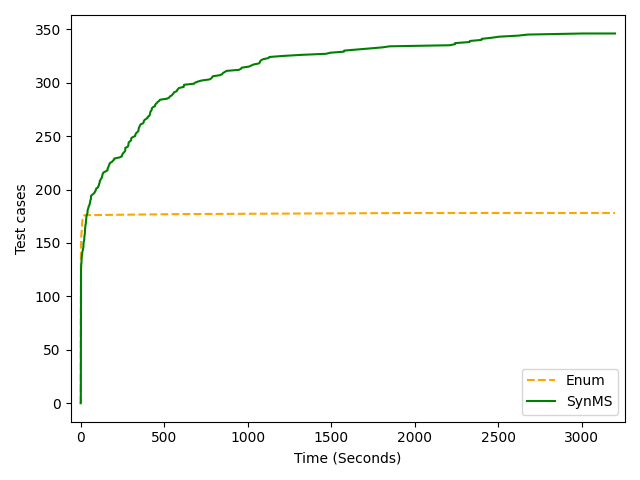
\includegraphics[width=\textwidth]{fig/misere-sub-f.png}
        \caption{Cumulative solved formula cases}
    \end{subfigure}
    \begin{subfigure}[b]{0.49\textwidth}
        \centering
        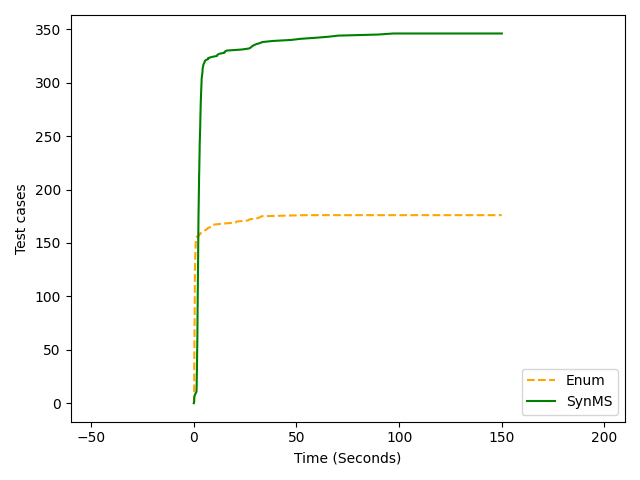
\includegraphics[width=\textwidth]{fig/misere-sub-s.png}
        \caption{Cumulative solved strategy cases}
    \end{subfigure}
    \caption{Cumulative solved test cases over time for Subtraction game under mis\`{e}re rule}
    \label{fig:misere-sub-line}
\end{figure}

\textbf{Comparison on Nim game.}
Table~\ref{tab:misere-nim-winFormulas}~presents the results for synthesizing winning formulas in the Nim game under the mis\`{e}re rule.
Out of $302$ test cases, Enum solves $38$ formula cases, while SynMS solves $85$, with success rates of $12.6\%$ and $28.1\%$, respectively.
Thus SynMS solves $47$ more formula cases than Enum.
The average formula synthesis time is $39.69$ seconds for Enum and $22.51$ seconds for SynMS.
Table~\ref{tab:misere-nim-winStrategies}~summarizes the corresponding results for synthesizing winning strategies.
Enum solves $36$ strategy cases, whereas SynMS solves $70$ strategy cases.
This gives SynMS an advantage of $34$ strategy cases in this benchmark group.
The average strategy synthesis time is $27.04$ seconds for Enum and $203.15$ seconds for SynMS.
In terms of solution size, Enum produces smaller formulas and strategies on average, with average sizes $7.05$ and $28.31$, while SynMS has average sizes $165.26$ and $2069.77$.
Figure~\ref{fig:misere-nim-line}~shows the cumulative number of solved test cases over time using the same solved-case filtering as the tables.

\begin{table*}[h!]
	%字体大小和行距
	\scriptsize
	%列距
	\setlength{\tabcolsep}{1pt}
	\centering
	\resizebox{\textwidth}{!}{%
	\renewcommand{\arraystretch}{1.12}%
	\begin{tabular}{|c|c|c|c|c|c|c|c|}
		\hline
		\multirow{3}{*}{Category} & \multirow{3}*{\tabincell{c}{Test \\ cases}} & \multicolumn{6}{c|}{Formula}  \\ \cline{3-8} &  & \multicolumn{2}{c|}{Solved} & \multicolumn{2}{c|}{Time} & \multicolumn{2}{c|}{Size} \\ \cline{3-8} & & \multicolumn{1}{c|}{Enum} & \multicolumn{1}{c|}{SynMS} & \multicolumn{1}{c|}{Enum} & \multicolumn{1}{c|}{SynMS} & \multicolumn{1}{c|}{Enum} & SynMS \\ \hline
		Nim & 7 & \textbf{1}(0) & \textbf{1}(0) & 5.51(5.51) & \textbf{1.36}(\textbf{1.36}) & \textbf{9.00}(\textbf{9.00}) & 28.00(28.00) \\ \hline
		Monotonic Nim & 7 & 4(1) & \textbf{5}(2) & 126.91(121.58) & \textbf{77.54}(\textbf{2.48}) & \textbf{8.00}(\textbf{6.67}) & 26.80(20.33) \\ \hline
		Empty and Transfer & 7 & 0(0) & \textbf{1}(1) & -(-) & 2.46(-) & -(-) & 70.00(-) \\ \hline
		Empty All But One & 6 & 0(0) & 0(0) & -(-) & -(-) & -(-) & -(-) \\ \hline
		Empty and Redistribute & 6 & 0(0) & \textbf{2}(2) & -(-) & 1.58(-) & -(-) & 132.00(-) \\ \hline
		Entropy Reduction Game & 7 & 0(0) & \textbf{1}(1) & -(-) & 13.56(-) & -(-) & 36.00(-) \\ \hline
		Min Game & 6 & 1(0) & \textbf{4}(3) & \textbf{3.42}(3.42) & 46.58(\textbf{3.07}) & \textbf{6.00}(\textbf{6.00}) & 249.25(15.00) \\ \hline
		$l$-Slow Nim & 180 & 7(0) & \textbf{15}(8) & \textbf{1.36}(\textbf{1.36}) & 70.67(5.37) & \textbf{4.71}(\textbf{4.71}) & 190.73(37.14) \\ \hline
		Sharing Nim & 7 & \textbf{4}(1) & \textbf{4}(1) & 11.22(14.75) & \textbf{7.48}(\textbf{5.92}) & \textbf{6.50}(\textbf{8.67}) & 27.00(29.33) \\ \hline
		Small Nim & 7 & 2(0) & \textbf{7}(5) & 92.79(92.79) & \textbf{1.65}(\textbf{0.98}) & 13.50(13.50) & \textbf{11.43}(\textbf{10.00}) \\ \hline
		Greedy Nim & 7 & 2(0) & \textbf{7}(5) & 103.30(103.30) & \textbf{3.34}(\textbf{1.07}) & \textbf{11.00}(\textbf{11.00}) & 336.43(49.00) \\ \hline
		Odd-or-Even Nim & 7 & 2(0) & \textbf{5}(3) & 18.96(18.96) & \textbf{1.05}(\textbf{0.92}) & \textbf{8.50}(\textbf{8.50}) & 377.60(66.00) \\ \hline
		Modular Nim & 5 & 1(0) & \textbf{2}(1) & \textbf{1.25}(\textbf{1.25}) & 1.53(1.52) & \textbf{4.00}(\textbf{4.00}) & 118.00(12.00) \\ \hline
		Pointed Nim & 7 & 0(0) & \textbf{4}(4) & -(-) & 11.49(-) & -(-) & 429.50(-) \\ \hline
		End Nim & 7 & 1(0) & \textbf{7}(6) & \textbf{2.74}(2.74) & 3.61(\textbf{1.01}) & \textbf{8.00}(\textbf{8.00}) & 295.00(\textbf{8.00}) \\ \hline
		Loop End Nim & 7 & 1(0) & \textbf{7}(6) & 34.66(34.66) & \textbf{9.10}(\textbf{5.81}) & \textbf{13.00}(\textbf{13.00}) & 113.57(45.00) \\ \hline
		Staircase Nim & 7 & \textbf{7}(0) & \textbf{7}(0) & 64.56(64.56) & \textbf{2.56}(\textbf{2.56}) & \textbf{6.86}(\textbf{6.86}) & 23.00(23.00) \\ \hline
		Circular Nim & 15 & 5(0) & \textbf{6}(1) & \textbf{3.30}(\textbf{3.30}) & 5.41(5.93) & \textbf{4.60}(\textbf{4.60}) & 41.83(26.00) \\ \hline
		Total & 302 & 38(2) & \textbf{85}(49) & 39.69(37.91) & \textbf{22.51}(\textbf{3.59}) & \textbf{7.05}(\textbf{7.11}) & 165.26(29.39) \\ \hline
	\end{tabular}%
	}
	\caption{Results of synthesizing winning formulas for Nim games under mis\`{e}re rule}
	\label{tab:misere-nim-winFormulas}
\end{table*}

\begin{table*}[h!]
	%字体大小和行距
	\scriptsize
	%列距
	\setlength{\tabcolsep}{1pt}
	\centering
	\resizebox{\textwidth}{!}{%
	\renewcommand{\arraystretch}{1.12}%
	\begin{tabular}{|c|c|c|c|c|c|c|c|}
		\hline
		\multirow{3}{*}{Category} & \multirow{3}*{\tabincell{c}{Test \\ cases}} & \multicolumn{6}{c|}{Strategy}  \\ \cline{3-8} &  & \multicolumn{2}{c|}{Solved} & \multicolumn{2}{c|}{Time} & \multicolumn{2}{c|}{Size} \\ \cline{3-8} & & \multicolumn{1}{c|}{Enum} & \multicolumn{1}{c|}{SynMS} & \multicolumn{1}{c|}{Enum} & \multicolumn{1}{c|}{SynMS} & \multicolumn{1}{c|}{Enum} & SynMS \\ \hline
		Nim & 7 & \textbf{1}(0) & \textbf{1}(0) & \textbf{2.08}(\textbf{2.08}) & 5.13(5.13) & \textbf{26.00}(\textbf{26.00}) & 138.00(138.00) \\ \hline
		Monotonic Nim & 7 & 4(1) & \textbf{5}(2) & \textbf{2.02}(\textbf{1.40}) & 33.12(29.32) & \textbf{34.75}(\textbf{26.67}) & 642.40(605.33) \\ \hline
		Empty and Transfer & 7 & 0(0) & \textbf{1}(1) & -(-) & 315.57(-) & -(-) & 52.00(-) \\ \hline
		Empty All But One & 6 & 0(0) & 0(0) & -(-) & -(-) & -(-) & -(-) \\ \hline
		Empty and Redistribute & 6 & 0(0) & 0(0) & -(-) & -(-) & -(-) & -(-) \\ \hline
		Entropy Reduction Game & 7 & 0(0) & 0(0) & -(-) & -(-) & -(-) & -(-) \\ \hline
		Min Game & 6 & 1(0) & \textbf{4}(3) & \textbf{0.49}(\textbf{0.49}) & 66.23(1.74) & \textbf{11.00}(\textbf{11.00}) & 1967.00(239.00) \\ \hline
		$l$-Slow Nim & 180 & 7(0) & \textbf{9}(2) & \textbf{0.37}(0.37) & 0.57(\textbf{0.19}) & \textbf{22.00}(\textbf{22.00}) & 621.78(141.43) \\ \hline
		Sharing Nim & 7 & \textbf{3}(2) & 2(1) & \textbf{0.24}(\textbf{0.71}) & 16.47(14.91) & \textbf{11.33}(\textbf{34.00}) & 958.00(960.00) \\ \hline
		Small Nim & 7 & 2(0) & \textbf{7}(5) & 1.40(\textbf{1.40}) & \textbf{0.85}(2.62) & \textbf{29.50}(\textbf{29.50}) & 30.00(30.00) \\ \hline
		Greedy Nim & 7 & 2(0) & \textbf{6}(4) & \textbf{2.01}(\textbf{2.01}) & 474.69(43.12) & \textbf{47.00}(\textbf{47.00}) & 3101.17(1963.50) \\ \hline
		Odd-or-Even Nim & 7 & 2(0) & \textbf{5}(3) & \textbf{0.66}(\textbf{0.66}) & 190.30(20.46) & \textbf{22.50}(\textbf{22.50}) & 1859.20(551.50) \\ \hline
		Modular Nim & 5 & 1(0) & \textbf{2}(1) & \textbf{0.54}(\textbf{0.54}) & 25.18(4.17) & \textbf{14.00}(\textbf{14.00}) & 267.00(32.00) \\ \hline
		Pointed Nim & 7 & 0(0) & \textbf{4}(4) & -(-) & 1004.20(-) & -(-) & 616.75(-) \\ \hline
		End Nim & 7 & 1(0) & \textbf{7}(6) & \textbf{1.25}(1.25) & 400.59(\textbf{0.05}) & \textbf{12.00}(\textbf{12.00}) & 12199.00(\textbf{12.00}) \\ \hline
		Loop End Nim & 7 & 1(0) & \textbf{6}(5) & \textbf{1.15}(1.15) & 181.08(\textbf{0.36}) & \textbf{16.00}(\textbf{16.00}) & 1215.33(18.00) \\ \hline
		Staircase Nim & 7 & \textbf{7}(0) & \textbf{7}(0) & \textbf{3.39}(\textbf{3.39}) & 44.26(44.26) & \textbf{49.00}(\textbf{49.00}) & 283.43(283.43) \\ \hline
		Circular Nim & 15 & \textbf{4}(0) & \textbf{4}(0) & \textbf{231.20}(\textbf{231.20}) & 339.47(339.47) & \textbf{18.00}(\textbf{18.00}) & 79.75(79.75) \\ \hline
		Total & 302 & 36(3) & \textbf{70}(37) & \textbf{27.04}(\textbf{29.38}) & 203.15(58.05) & \textbf{28.31}(\textbf{29.09}) & 2069.77(351.45) \\ \hline
	\end{tabular}%
	}
	\caption{Results of synthesizing winning strategies for Nim games under mis\`{e}re rule}
	\label{tab:misere-nim-winStrategies}
\end{table*}

\begin{figure}[h!]
    \centering
    \begin{subfigure}[b]{0.49\textwidth}
        \centering
        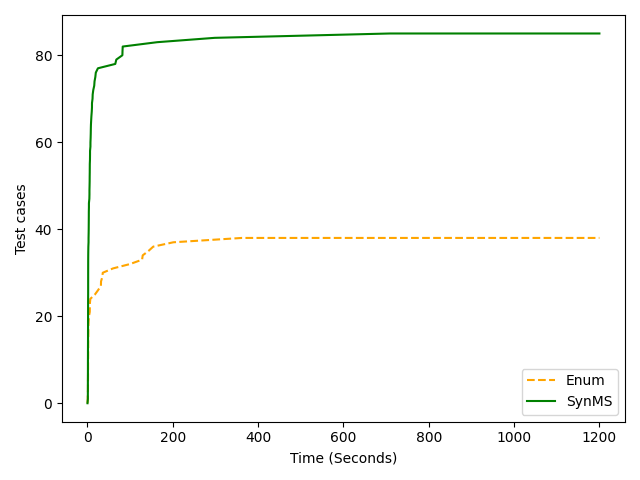
\includegraphics[width=\textwidth]{fig/misere-nim-f.png}
        \caption{Cumulative solved formula cases}
    \end{subfigure}
    \begin{subfigure}[b]{0.49\textwidth}
        \centering
        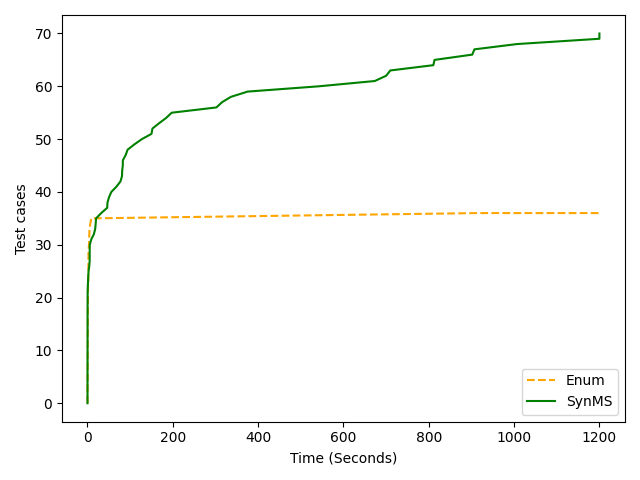
\includegraphics[width=\textwidth]{fig/misere-nim-s.png}
        \caption{Cumulative solved strategy cases}
    \end{subfigure}
    \caption{Cumulative solved test cases over time for Nim game under mis\`{e}re rule}
    \label{fig:misere-nim-line}
\end{figure}

\textbf{Comparison on Welter game.}
Table~\ref{tab:misere-welter-winFormulas}~presents the results for synthesizing winning formulas in the Welter game under the mis\`{e}re rule.
Out of $7$ test cases, Enum solves $2$ formula cases, while SynMS solves $7$, with success rates of $28.6\%$ and $100.0\%$, respectively.
Thus SynMS solves $5$ more formula cases than Enum.
The average formula synthesis time is $1.62$ seconds for Enum and $158.34$ seconds for SynMS.
Table~\ref{tab:misere-welter-winStrategies}~summarizes the corresponding results for synthesizing winning strategies.
Enum solves $2$ strategy cases, whereas SynMS solves $5$ strategy cases.
This gives SynMS an advantage of $3$ strategy cases in this benchmark group.
The average strategy synthesis time is $0.65$ seconds for Enum and $7.97$ seconds for SynMS.
In terms of solution size, Enum produces smaller formulas and strategies on average, with average sizes $4.50$ and $43.00$, while SynMS has average sizes $263.14$ and $535.60$.
Figure~\ref{fig:misere-welter-line}~shows the cumulative number of solved test cases over time using the same solved-case filtering as the tables.

\begin{table*}[h!]
	%字体大小和行距
	\footnotesize
	%列距
	\setlength{\tabcolsep}{3pt}
	\centering
	\resizebox{\textwidth}{!}{%
	\renewcommand{\arraystretch}{1.12}%
	\begin{tabular}{|c|c|c|c|c|c|c|c|}
		\hline
		\multirow{3}{*}{Category} & \multirow{3}*{\tabincell{c}{Test \\ cases}} & \multicolumn{6}{c|}{Formula}  \\ \cline{3-8} &  & \multicolumn{2}{c|}{Solved} & \multicolumn{2}{c|}{Time} & \multicolumn{2}{c|}{Size} \\ \cline{3-8} & & \multicolumn{1}{c|}{Enum} & \multicolumn{1}{c|}{SynMS} & \multicolumn{1}{c|}{Enum} & \multicolumn{1}{c|}{SynMS} & \multicolumn{1}{c|}{Enum} & SynMS \\ \hline
		Welter & 1 & 0(0) & \textbf{1}(1) & -(-) & 1.89(-) & -(-) & 570.00(-) \\ \hline
		$l$-Welter & 5 & 2(0) & \textbf{5}(3) & \textbf{1.62}(\textbf{1.62}) & 221.01(3.53) & \textbf{4.50}(\textbf{4.50}) & 240.00(114.00) \\ \hline
		Max-Welter & 1 & 0(0) & \textbf{1}(1) & -(-) & 1.48(-) & -(-) & 72.00(-) \\ \hline
		Total & 7 & 2(0) & \textbf{7}(5) & \textbf{1.62}(\textbf{1.62}) & 158.34(3.53) & \textbf{4.50}(\textbf{4.50}) & 263.14(114.00) \\ \hline
	\end{tabular}%
	}
	\caption{Results of synthesizing winning formulas for Welter games under mis\`{e}re rule}
	\label{tab:misere-welter-winFormulas}
\end{table*}

\begin{table*}[h!]
	%字体大小和行距
	\footnotesize
	%列距
	\setlength{\tabcolsep}{3pt}
	\centering
	\resizebox{\textwidth}{!}{%
	\renewcommand{\arraystretch}{1.12}%
	\begin{tabular}{|c|c|c|c|c|c|c|c|}
		\hline
		\multirow{3}{*}{Category} & \multirow{3}*{\tabincell{c}{Test \\ cases}} & \multicolumn{6}{c|}{Strategy}  \\ \cline{3-8} &  & \multicolumn{2}{c|}{Solved} & \multicolumn{2}{c|}{Time} & \multicolumn{2}{c|}{Size} \\ \cline{3-8} & & \multicolumn{1}{c|}{Enum} & \multicolumn{1}{c|}{SynMS} & \multicolumn{1}{c|}{Enum} & \multicolumn{1}{c|}{SynMS} & \multicolumn{1}{c|}{Enum} & SynMS \\ \hline
		Welter & 1 & 0(0) & \textbf{1}(1) & -(-) & 32.12(-) & -(-) & 190.00(-) \\ \hline
		$l$-Welter & 5 & 2(0) & \textbf{3}(1) & \textbf{0.65}(\textbf{0.65}) & 0.73(0.74) & \textbf{43.00}(\textbf{43.00}) & 817.33(784.00) \\ \hline
		Max-Welter & 1 & 0(0) & \textbf{1}(1) & -(-) & 5.57(-) & -(-) & 36.00(-) \\ \hline
		Total & 7 & 2(0) & \textbf{5}(3) & \textbf{0.65}(\textbf{0.65}) & 7.97(0.74) & \textbf{43.00}(\textbf{43.00}) & 535.60(784.00) \\ \hline
	\end{tabular}%
	}
	\caption{Results of synthesizing winning strategies for Welter games under mis\`{e}re rule}
	\label{tab:misere-welter-winStrategies}
\end{table*}

\begin{figure}[h!]
    \centering
    \begin{subfigure}[b]{0.49\textwidth}
        \centering
        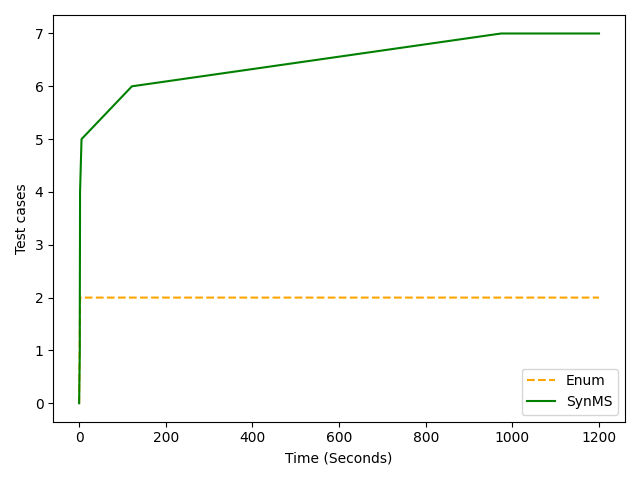
\includegraphics[width=\textwidth]{fig/misere-welter-f.png}
        \caption{Cumulative solved formula cases}
    \end{subfigure}
    \begin{subfigure}[b]{0.49\textwidth}
        \centering
        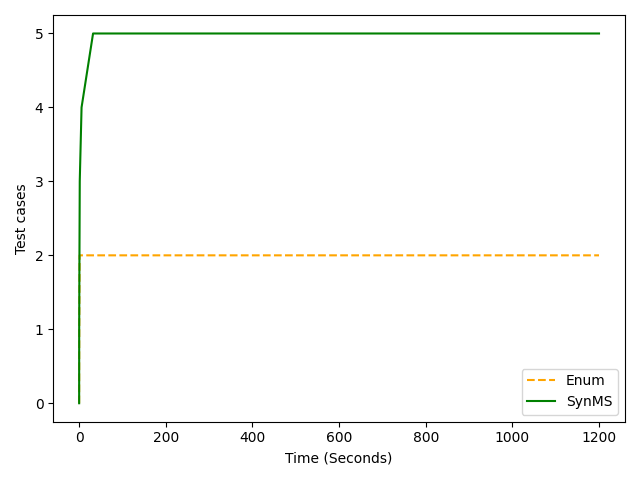
\includegraphics[width=\textwidth]{fig/misere-welter-s.png}
        \caption{Cumulative solved strategy cases}
    \end{subfigure}
    \caption{Cumulative solved test cases over time for Welter game under mis\`{e}re rule}
    \label{fig:misere-welter-line}
\end{figure}

\textbf{Comparison on Wythoff game.}
Table~\ref{tab:misere-wythoff-winFormulas}~presents the results for synthesizing winning formulas in the Wythoff game under the mis\`{e}re rule.
Out of $2924$ test cases, Enum solves $1933$ formula cases, while SynMS solves $2691$, with success rates of $66.1\%$ and $92.0\%$, respectively.
Thus SynMS solves $758$ more formula cases than Enum.
The average formula synthesis time is $37.54$ seconds for Enum and $27.52$ seconds for SynMS.
Table~\ref{tab:misere-wythoff-winStrategies}~summarizes the corresponding results for synthesizing winning strategies.
Enum solves $1919$ strategy cases, whereas SynMS solves $2420$ strategy cases.
This gives SynMS an advantage of $501$ strategy cases in this benchmark group.
The average strategy synthesis time is $18.84$ seconds for Enum and $386.13$ seconds for SynMS.
In terms of solution size, Enum produces smaller formulas and strategies on average, with average sizes $6.73$ and $42.58$, while SynMS has average sizes $72.72$ and $453.61$.
Figure~\ref{fig:misere-wythoff-line}~shows the cumulative number of solved test cases over time using the same solved-case filtering as the tables.

\begin{table*}[h!]
	%字体大小和行距
	\tiny
	%列距
	\setlength{\tabcolsep}{0.8pt}
	\centering
	\resizebox{\textwidth}{!}{%
	\renewcommand{\arraystretch}{1.12}%
	\begin{tabular}{|c|c|c|c|c|c|c|c|}
		\hline
		\multirow{3}{*}{Category} & \multirow{3}*{\tabincell{c}{Test \\ cases}} & \multicolumn{6}{c|}{Formula}  \\ \cline{3-8} &  & \multicolumn{2}{c|}{Solved} & \multicolumn{2}{c|}{Time} & \multicolumn{2}{c|}{Size} \\ \cline{3-8} & & \multicolumn{1}{c|}{Enum} & \multicolumn{1}{c|}{SynMS} & \multicolumn{1}{c|}{Enum} & \multicolumn{1}{c|}{SynMS} & \multicolumn{1}{c|}{Enum} & SynMS \\ \hline
		Wythoff & 21 & 10(0) & \textbf{19}(9) & 41.51(41.51) & \textbf{2.57}(\textbf{2.89}) & \textbf{6.60}(\textbf{6.60}) & 152.95(35.30) \\ \hline
		$l$-Wythoff & 140 & 80(0) & \textbf{123}(43) & 48.85(48.85) & \textbf{46.97}(\textbf{2.95}) & \textbf{7.21}(\textbf{7.21}) & 75.62(45.55) \\ \hline
		Monotonic $l$-Diet Wythoff & 105 & 61(0) & \textbf{104}(43) & 31.07(31.07) & \textbf{11.34}(\textbf{2.98}) & \textbf{5.28}(\textbf{5.28}) & 66.65(15.21) \\ \hline
		Wythoff with subtraction set $S$ & 315 & 200(0) & \textbf{287}(87) & 24.59(24.59) & \textbf{4.75}(\textbf{2.62}) & \textbf{6.28}(\textbf{6.28}) & 106.17(38.67) \\ \hline
		Wythoff with a function $f$ & 168 & 116(0) & \textbf{153}(37) & 38.93(38.93) & \textbf{6.13}(\textbf{3.23}) & \textbf{7.37}(\textbf{7.37}) & 63.46(39.89) \\ \hline
		1st($l_1$,$l_2$)\-restricted Wythoff & 315 & 214(0) & \textbf{285}(71) & 26.60(26.60) & \textbf{2.26}(\textbf{2.37}) & \textbf{6.83}(\textbf{6.83}) & 99.46(48.95) \\ \hline
		2nd($l_1$,$l_2$)\-restricted Wythoff & 600 & 440(0) & \textbf{600}(160) & 37.98(37.98) & \textbf{2.80}(\textbf{2.39}) & \textbf{6.36}(\textbf{6.36}) & 59.01(34.23) \\ \hline
		3rd($l_1$,$l_2$)\-restricted Wythoff & 700 & 404(1) & \textbf{588}(185) & \textbf{55.56}(55.67) & 96.15(\textbf{4.50}) & \textbf{7.18}(\textbf{7.17}) & 54.75(44.65) \\ \hline
		4th($l_1$,$l_2$)\-restricted Wythoff & 560 & 408(0) & \textbf{532}(124) & 29.58(29.58) & \textbf{11.05}(\textbf{3.67}) & \textbf{6.80}(\textbf{6.80}) & 76.01(34.99) \\ \hline
		Total & 2924 & 1933(1) & \textbf{2691}(759) & 37.54(37.56) & \textbf{27.52}(\textbf{3.21}) & \textbf{6.73}(\textbf{6.73}) & 72.72(38.87) \\ \hline
	\end{tabular}%
	}
	\caption{Results of synthesizing winning formulas for Wythoff games under mis\`{e}re rule}
	\label{tab:misere-wythoff-winFormulas}
\end{table*}

\begin{table*}[h!]
	%字体大小和行距
	\tiny
	%列距
	\setlength{\tabcolsep}{0.8pt}
	\centering
	\resizebox{\textwidth}{!}{%
	\renewcommand{\arraystretch}{1.12}%
	\begin{tabular}{|c|c|c|c|c|c|c|c|}
		\hline
		\multirow{3}{*}{Category} & \multirow{3}*{\tabincell{c}{Test \\ cases}} & \multicolumn{6}{c|}{Strategy}  \\ \cline{3-8} &  & \multicolumn{2}{c|}{Solved} & \multicolumn{2}{c|}{Time} & \multicolumn{2}{c|}{Size} \\ \cline{3-8} & & \multicolumn{1}{c|}{Enum} & \multicolumn{1}{c|}{SynMS} & \multicolumn{1}{c|}{Enum} & \multicolumn{1}{c|}{SynMS} & \multicolumn{1}{c|}{Enum} & SynMS \\ \hline
		Wythoff & 21 & 10(1) & \textbf{16}(7) & \textbf{1.56}(\textbf{1.42}) & 21.65(6.15) & \textbf{31.40}(\textbf{28.22}) & 278.56(127.89) \\ \hline
		$l$-Wythoff & 140 & 80(8) & \textbf{102}(30) & \textbf{5.62}(\textbf{3.12}) & 663.64(580.49) & \textbf{54.11}(\textbf{48.61}) & 790.93(343.90) \\ \hline
		Monotonic $l$-Diet Wythoff & 105 & 61(7) & \textbf{95}(41) & \textbf{0.44}(0.49) & 0.50(\textbf{0.16}) & \textbf{22.03}(\textbf{24.89}) & 419.32(76.31) \\ \hline
		Wythoff with subtraction set $S$ & 315 & 200(5) & \textbf{266}(71) & \textbf{1.70}(\textbf{1.62}) & 25.91(7.60) & \textbf{30.09}(\textbf{29.21}) & 368.59(166.89) \\ \hline
		Wythoff with a function $f$ & 168 & 116(1) & \textbf{140}(25) & \textbf{3.54}(\textbf{3.55}) & 442.66(384.41) & \textbf{52.01}(\textbf{51.94}) & 598.21(483.18) \\ \hline
		1st($l_1$,$l_2$)\-restricted Wythoff & 315 & 214(5) & \textbf{264}(55) & \textbf{2.38}(\textbf{2.29}) & 16.59(10.67) & \textbf{37.33}(\textbf{36.46}) & 365.79(238.08) \\ \hline
		2nd($l_1$,$l_2$)\-restricted Wythoff & 600 & 440(41) & \textbf{538}(139) & \textbf{2.52}(\textbf{2.68}) & 705.10(499.45) & \textbf{43.83}(\textbf{46.91}) & 328.33(242.01) \\ \hline
		3rd($l_1$,$l_2$)\-restricted Wythoff & 700 & 404(40) & \textbf{499}(135) & \textbf{12.26}(\textbf{7.91}) & 723.65(662.59) & \textbf{59.64}(\textbf{55.02}) & 562.53(358.20) \\ \hline
		4th($l_1$,$l_2$)\-restricted Wythoff & 560 & 394(7) & \textbf{500}(113) & \textbf{71.94}(\textbf{2.68}) & 105.31(51.97) & \textbf{31.03}(\textbf{31.03}) & 474.15(316.60) \\ \hline
		Total & 2924 & 1919(115) & \textbf{2420}(616) & \textbf{18.84}(\textbf{3.58}) & 386.13(305.07) & \textbf{42.58}(\textbf{41.65}) & 453.61(286.79) \\ \hline
	\end{tabular}%
	}
	\caption{Results of synthesizing winning strategies for Wythoff games under mis\`{e}re rule}
	\label{tab:misere-wythoff-winStrategies}
\end{table*}

\begin{figure}[h!]
    \centering
    \begin{subfigure}[b]{0.49\textwidth}
        \centering
        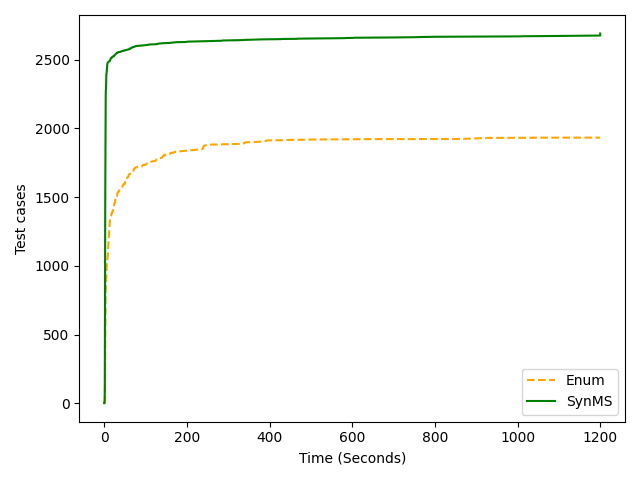
\includegraphics[width=\textwidth]{fig/misere-wythoff-f.png}
        \caption{Cumulative solved formula cases}
    \end{subfigure}
    \begin{subfigure}[b]{0.49\textwidth}
        \centering
        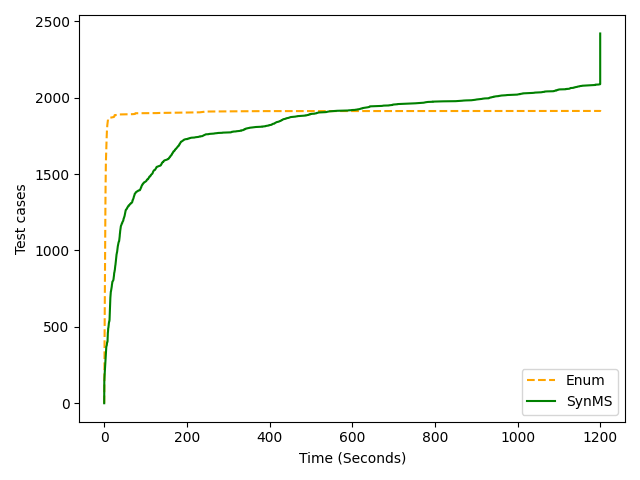
\includegraphics[width=\textwidth]{fig/misere-wythoff-s.png}
        \caption{Cumulative solved strategy cases}
    \end{subfigure}
    \caption{Cumulative solved test cases over time for Wythoff game under mis\`{e}re rule}
    \label{fig:misere-wythoff-line}
\end{figure}

\textbf{Comparison on Chomp game.}
Table~\ref{tab:misere-chomp-winFormulas}~presents the results for synthesizing winning formulas in the Chomp game under the mis\`{e}re rule.
Out of $8$ test cases, Enum solves $2$ formula cases, while SynMS solves $3$, with success rates of $25.0\%$ and $37.5\%$, respectively.
Thus SynMS solves $1$ more formula cases than Enum.
The average formula synthesis time is $17.48$ seconds for Enum and $4.66$ seconds for SynMS.
Table~\ref{tab:misere-chomp-winStrategies}~summarizes the corresponding results for synthesizing winning strategies.
Enum solves $2$ strategy cases, whereas SynMS solves $2$ strategy cases.
Both approaches solve $2$ strategy cases in this benchmark group.
The average strategy synthesis time is $3.33$ seconds for Enum and $5.17$ seconds for SynMS.
In terms of solution size, the average formula size is $6.00$ for Enum and $62.33$ for SynMS, and the average strategy size is $45.50$ for Enum and $24.00$ for SynMS.
Figure~\ref{fig:misere-chomp-line}~shows the cumulative number of solved test cases over time using the same solved-case filtering as the tables.

\begin{table*}[h!]
	%字体大小和行距
	\footnotesize
	%列距
	\setlength{\tabcolsep}{3pt}
	\centering
	\resizebox{\textwidth}{!}{%
	\renewcommand{\arraystretch}{1.12}%
	\begin{tabular}{|c|c|c|c|c|c|c|c|}
		\hline
		\multirow{3}{*}{Category} & \multirow{3}*{\tabincell{c}{Test \\ cases}} & \multicolumn{6}{c|}{Formula}  \\ \cline{3-8} &  & \multicolumn{2}{c|}{Solved} & \multicolumn{2}{c|}{Time} & \multicolumn{2}{c|}{Size} \\ \cline{3-8} & & \multicolumn{1}{c|}{Enum} & \multicolumn{1}{c|}{SynMS} & \multicolumn{1}{c|}{Enum} & \multicolumn{1}{c|}{SynMS} & \multicolumn{1}{c|}{Enum} & SynMS \\ \hline
		Chomp & 7 & 1(0) & \textbf{2}(1) & \textbf{1.49}(\textbf{1.49}) & 6.09(1.75) & \textbf{3.00}(\textbf{3.00}) & 79.50(40.00) \\ \hline
		L-shaped Chomp & 1 & \textbf{1}(0) & \textbf{1}(0) & 33.46(33.46) & \textbf{1.81}(\textbf{1.81}) & \textbf{9.00}(\textbf{9.00}) & 28.00(28.00) \\ \hline
		Total & 8 & 2(0) & \textbf{3}(1) & 17.48(17.48) & \textbf{4.66}(\textbf{1.78}) & \textbf{6.00}(\textbf{6.00}) & 62.33(34.00) \\ \hline
	\end{tabular}%
	}
	\caption{Results of synthesizing winning formulas for Chomp games under mis\`{e}re rule}
	\label{tab:misere-chomp-winFormulas}
\end{table*}

\begin{table*}[h!]
	%字体大小和行距
	\footnotesize
	%列距
	\setlength{\tabcolsep}{3pt}
	\centering
	\resizebox{\textwidth}{!}{%
	\renewcommand{\arraystretch}{1.12}%
	\begin{tabular}{|c|c|c|c|c|c|c|c|}
		\hline
		\multirow{3}{*}{Category} & \multirow{3}*{\tabincell{c}{Test \\ cases}} & \multicolumn{6}{c|}{Strategy}  \\ \cline{3-8} &  & \multicolumn{2}{c|}{Solved} & \multicolumn{2}{c|}{Time} & \multicolumn{2}{c|}{Size} \\ \cline{3-8} & & \multicolumn{1}{c|}{Enum} & \multicolumn{1}{c|}{SynMS} & \multicolumn{1}{c|}{Enum} & \multicolumn{1}{c|}{SynMS} & \multicolumn{1}{c|}{Enum} & SynMS \\ \hline
		Chomp & 7 & \textbf{1}(0) & \textbf{1}(0) & \textbf{5.28}(\textbf{5.28}) & 7.79(7.79) & 65.00(65.00) & \textbf{14.00}(\textbf{14.00}) \\ \hline
		L-shaped Chomp & 1 & \textbf{1}(0) & \textbf{1}(0) & \textbf{1.38}(\textbf{1.38}) & 2.54(2.54) & \textbf{26.00}(\textbf{26.00}) & 34.00(34.00) \\ \hline
		Total & 8 & \textbf{2}(0) & \textbf{2}(0) & \textbf{3.33}(\textbf{3.33}) & 5.17(5.17) & 45.50(45.50) & \textbf{24.00}(\textbf{24.00}) \\ \hline
	\end{tabular}%
	}
	\caption{Results of synthesizing winning strategies for Chomp games under mis\`{e}re rule}
	\label{tab:misere-chomp-winStrategies}
\end{table*}

\begin{figure}[h!]
    \centering
    \begin{subfigure}[b]{0.49\textwidth}
        \centering
        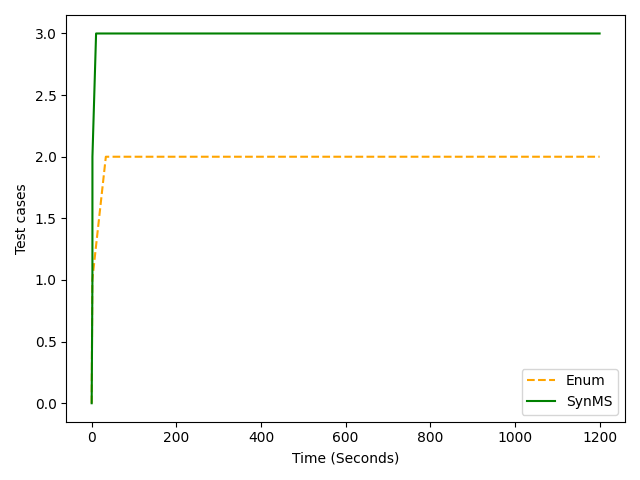
\includegraphics[width=\textwidth]{fig/misere-chomp-f.png}
        \caption{Cumulative solved formula cases}
    \end{subfigure}
    \begin{subfigure}[b]{0.49\textwidth}
        \centering
        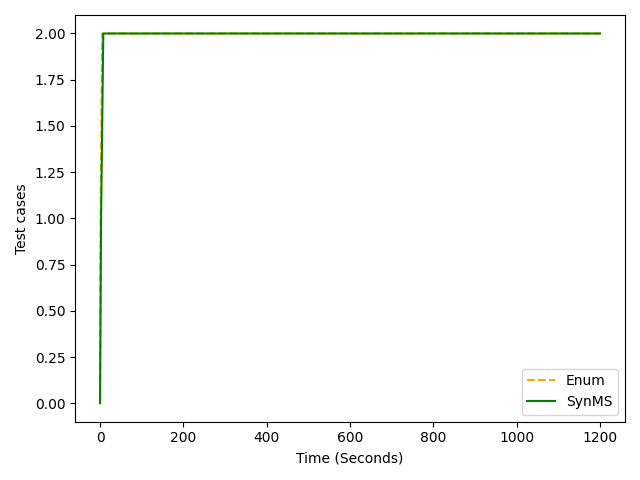
\includegraphics[width=\textwidth]{fig/misere-chomp-s.png}
        \caption{Cumulative solved strategy cases}
    \end{subfigure}
    \caption{Cumulative solved test cases over time for Chomp game under mis\`{e}re rule}
    \label{fig:misere-chomp-line}
\end{figure}

\section{Related work}
\subsection{Theoretical results on ICGs}

\subsubsection{Winning and losing states}
\looseness=-1
Identifying the exact set of winning (or losing) states is one of the longstanding and central problems in the study of ICGs.
For example, several variants of Nim game admit elegant characterizations of their losing states.
In End Nim, a state is losing iff all piles have the same even number of chips \cite{AlbN2001}.
In Greedy Nim, a state is losing iff the number of equal largest piles is even \cite{AlbN2004}.
For Odd-or-Even Nim game, when previous player specifies the even constraint for the next player, a state is losing iff $v_1 \lxor \cdots \lxor v_n \in{0, 1}$ where $\lxor$ denotes the bitwise exclusive-or operator \cite{SmiS2002}.
When the odd constraint is specified, a state is losing iff the number of chips in every pile are all even and $v_1 \lxor \cdots \lxor v_n = 0$.
Circular Nim provides another family of Nim variants with more complex structures.
Let $CN(n, k)$ ($SCN(n, k)$) denote a (Shrinking) Circular Nim game with $n$ piles in which a player can reduce $k$ consecutive piles.
The two Circular Nim $CN(n, 1)$ and $CN(n, n - 1)$ are two special cases of Moore Nim game \cite{Moo1910}, a generalization of the classical Nim game in which a player is allowed to remove chips from multiple piles in a single move.
The losing states of several (Shrinking) Circular Nim variants was characterized, including $CN(5, 3)$,  $CN(6, 4)$, $CN(7, 4)$ $CN(8, 6)$, $SCN(5, 2)$, $SCN(5, 3)$ \cite{DufH2013,DufHV2021,OgiS2025}.


\looseness=-1
Besides Mark game \cite{Kru2009}, there are some LIA-definable ICGs whose sets of losing states are not LIA-definable.
One such example is Wythoff game, whose losing states are characterized by a Beatty sequence $(\largestInt[g \cdot n], \largestInt[g^2 \cdot n])$ where $g$ is the Golden ratio $\frac{1 + \sqrt{5}}{2}$ and $\largestInt[r]$ is the integer part of the real number $r$ \cite{Ray1894,Bea1926}.
The projection of the above Beatty sequence onto either coordinate is aperiodic, and hence not LIA-definable.
Since LIA-definable relations are closed under projection, the set of losing states of Wythoff game is not LIA-definable.
Another example is Fibonaci Nim, an extension of one-pile Nim game proposed by \citet{Whi1963}, in which a player can take at most twice as many chips as the previous move.
\citet{Whi1963} proved that a state $(v, m)$ where $v$ is the number of remaining chips and $m$ is the maximum number of chips the current player can take is a losing state iff $m < z_1(v)$ where $z_1(v)$ is the smallest Fibonacci number in the Zeckendorf representation \cite{Zec1972} of $v$.
The set $S$ of pairs $(v, v - 1)$ of integers s.t. $v$ is odd clearly is LIA-definable.
The intersection of $S$ and the set of losing states in Fibonaci Nim is $(F_k, F_k - 1)$ where $F_k$ is the $k$-th Fibonacci number and $F_k$ is odd, and its projection onto the first coordinate is the set of odd Fibonacci numbers, which is not ultimately periodic.
Since LIA-definable sets are closed under intersection and projection, the set of losing states of Fibonaci Nim game is not LIA-definable.
%\cite{Lev2006,MiyM2023}

\looseness=-1
\citet{LarW2013} proved that the problem of deciding whether two LIA-definable ICGs have the same set of winning states is undecidable.	
Subsequently, \citet{Lar2013} showed that, for an LIA-definable ICG with $2$ state variables, it is undecidable to decide whether its set of winning states is $2$-dimensional ultimately periodic.
Formally, a set $S \subseteq \intNum^2$ is $2$-dimensional linear with a single period, iff there are two vectors $\vec{z}$ and $\vec{z}_1$ s.t. $\vec{z} \in S$ iff $\vec{z} + \lambda_1 \vec{z}_1 \in S$ for any $\lambda_1 \in \intNum$.
A set $S \subseteq \intNum^2$ is $2$-dimensional semi-linear with a single period iff it is a finite union of $2$-dimensional linear with a single period sets.
Even in sets of $2$-dimensional integers, semi-linearity is a weaker property than $2$-dimensional semi-linearity with a single period. 
Later, ?? extended the undecidability results in \citet{Lar2013} to semi-linearity, that is, the problem of deciding whether the set of winning states for an LIA-definable ICG is LIA-definable is undecidable.


\subsubsection{Sprague-Grundy function}
\looseness=-1
Sprague-Grundy function is a more fine-grained notion than winning and losing states, and is used to study the compound of multiple ICGs under the normal play rule \cite{Spr1935,Gru1939}.
Given a set of ICGs $\Pi_1, \cdots, \Pi_n$, their disjuntive compound, denoted by $\Pi_1 + \cdots + \Pi_n$, is an ICG where each player choose only one game $\Pi_i$ and execute an possible action in such game in each turn.
The Sprague-Grundy value $G(s)$ of a state $s$ is recursively defined as 
\[G(s) = \min\set{n \geq 0 \mid n \neq G(s') \text{ for every successor state } s' \text{ of } s}. \]
In a word, $G(s)$ is the smallest non-negative integer not found among the Sprague-Grundy values of the successors of $s$.
Under the normal play rule, a state $s$ is losing iff $G(s) = 0$.
\citet{Bou1901} proved that for all individual Nim games $\Pi_1, \cdots, \Pi_n$, $G((s_1, \cdots, s_n)) = G(s_1) \lxor \cdots \lxor G(s_n)$ where $\lxor$ is the bitwise exclusive-or operator, each $s_i$ is a legal state of $\Pi_i$, and $(s_1, \cdots, s_n)$ is a compound state of $\Pi_1 + \cdots + \Pi_n$.
The above theoretical result was generalized to arbitrary ICGs independently by \citet{Spr1935} and \citet{Gru1939}.
Therefore, every state in any ICG is equivalent to a state in one-pile Nim game.

\looseness=-1
Closed form of Sprague–Grundy functions are known for several ICGs and their variants.
The Sprague–Grundy function $G(v)$ of Take-away game satisfies the condition $G(v) \modulo_{m + 1} v$ where $v$ is the number of remaining chips and $m$ is the maximum number $m$ of chips that can be removed \cite{Gol1966}.
An extension to Nim game, namely Proper Nim \cite{JenM1980}, allows a player to take chips from more than one piles but not all piles simultaneously.
This game is equivalent to the Circular Nim $CN(n, n - 1)$.
\citet{BorGHM2021} obtained the Sprague–Grundy function for Proper Nim with at least $3$ piles: $G((v_1, \cdots, v_m)) = \sum_{i = 1}^m v_i$.
\citet{BorGHMM2018} introduced another extension, called Exact $k$-Nim, requiring a player to remove chips from exactly $k$ piles, and provided the explicit form of Sprague–Grundy function for Exact $k$-Nim with $n$ piles when $n \leq 2k$. 
Euclid game is defined on a pair $(v_1, v_2)$ of non-negative integers \cite{ColD1969}.
In each move, a player subtracts from the larger integer a positive integer multiple of the smaller one as long as it is still positive.
The game ends when either $v_1$ or $v_2$ becomes $0$.
\citet{Gro1997} introduced a subtle variation of Euclid game in which it ends when $v_1 = v_2$.
The original Euclid and Grossman's variation have the same set of losing states. 
Specially, for $v_1 < v_2$, $(v_1, v_2)$ is a losing state iff $v_2 < g \cdot v_1$ where $g$ is the golden ratio, and a symmetric condition holds for $v_2 > v_1$ \cite{ColD1969,Str1998}.
However, their Sprague–Grundy functions are different.
For $v_2 > v_1 > 0$, the Sprague–Grundy function of the original Euclid game, given by \citet{CaiHL2011}, is
\begin{center}
	$G(v_1, v_2) = \begin{cases}
		\left\lfloor \dfrac{v_2}{v_1} \right \rfloor - 1, & \text{if } l(v_1, v_2) \text{ is even}; \\
		\left\lfloor \dfrac{v_2}{v_1} \right \rfloor,  & \text{otherwise}.
	\end{cases}
	$
\end{center}
where $l(v_1, v_2)$ is the the largest nonnegative integer $i$ s.t. $a_0 = a_1 = \cdots = a_{i - 1} < a_i$ and $\dfrac{v_2}{v_1} = a_0 + \dfrac{1}{a_1 + \dfrac{1}{\ddots a_{n - 1} + \dfrac{1}{a_n}}}$.
The Sprague–Grundy function of Grossman's Euclid game is relatively simple: $G(v_1, v_2) = \left\lfloor \left\lvert \dfrac{v_1}{v_2} - \dfrac{v_2}{v_1} \right\rvert \right \rfloor$ \cite{Niv2006}.
In addition, \citet{Byr2003} proved the periodicity of the Sprague-Grundy value for states of Chomp in which the numbers of chips in all rows except the first two are fixed.
Formally, $G((v_1, v_2, v_3, v_4, \cdots)) = G((v_1 + p, v_2 + p, v_3, v_4, \cdots))$ where $v_i$ denotes the number of chips in the $i$-th row and $p$ is the period.

\looseness=-1
However, Sprague-Grundy function are not suitable for analyzing the disjunctive compound of ICGs under the mis\`{e}re play rule.
To address this issue, \citet{PlaS2008} adopted the notion of commutative monoids $(S, +, e)$ (that is, a set $S$ equipped with an commutative and associative binary operation $+$ and an identity element $e$) instead of Sprague-Grundy values to encode the additive structure of ICGs under the mis\`{e}re play rule.
They defined a mapping $\Phi$ that assigns every state $s$ an element $\Phi(s) \in S$, together with a subset $S_{\loseSet} \subset S$ s.t. $s$ is a losing state iff $\Phi(s) \in S_{\loseSet}$.
For a disjuntive compound $\Pi_1 + \cdots + \Pi_n$ where all $\Pi_i$'s are associated with the same commutative monoid, a compound state $(s_1, \cdots, s_n)$ is losing iff $\Phi(s_1) + \cdots + \Phi(s_n) \in S_{\loseSet}$.
Clearly, $(\intNum^{0+}, +, 0)$ is a commutative monoid where $\intNum^{0+}$ is the set of non-negative integers.
Hence, Sprague--Grundy values can be viewed as a special case of the commutative monoid.

\looseness=-1
By incorporating a set of infinite cardinals (that is, numbers larger than all integers), three different generalizations of Sprague-Grundy value were proposed to accommodate cyclic ICGs over finite graphs \cite{Smith1966,FraP1975,FraT1975,Con1976,FraY1982}.
\citet{FraY1986} established that (1) the above three generalized definitions are equivalent; (2) there is a unique generalized Sprague-Grundy function; (3) the Sprague-Grundy value for every state can be computed in polynomial time.
Subsequently, these results were extended to two classes of ICGs over infinite graphs: locally path-bounded graphs (that is, the length of every path starting from any vertex is bounded) \cite{FraR2001} and locally finite graphs (that is, each vertex has finitely many successors) \cite{Mar2021}.

%\citet{Moo1910} proposed a more general compound of Nim game, namely Moore Nim, which allows a player chooses at most $k$ piles.



%\looseness=-1
%Sprague-Grundy theory has supported both analytical and computational studies. 
%%On the analytical side, many works study the exact Sprague-Grundy function or its regularities for specific games, such as Euclid \cite{cairns2011,nivasch2006}, Wythoff's game \cite{blass1990}, and Grundy's game \cite{guy1956g}. 
%Another recurring topic is the periodicity of nim-values, for example in peg duotaire \cite{grossman2004}. 
%These results reveal deep mathematical structure, but they are usually game specific and rely on substantial manual analysis.
%
%\looseness=-1
%On the computational side, several works aim to accelerate the recursive evaluation of Sprague-Grundy values. 
%\citet{lemoine2012} computes Sprague-Grundy values by reducing candidate values to losing position tests in suitable sum games. 
%%\citet{BelM2020} adapt $\alpha$-$\beta$ style pruning to the mex computation itself, thereby reducing the search effort required for impartial games. 
%An additional direction combines Sprague-Grundy values with search in decomposable positions. 
%\citet{muller1999} proposed decomposition search for Go endgames. 
%\citet{uiterwijk2019} applied a related idea to Cram, a domino-placement impartial game. 
%His method combines combinatorial game theory with transposition tables and endgame databases, which are precomputed repositories of exact values for small remaining board positions. 
%Once a searched position can be decomposed into smaller components or matched with a stored endgame position, the solver can reuse the known values and avoid further exhaustive search.

\subsubsection{Remoteness function}
In addition to Sprague-Grundy function, the notion of remoteness function dates back to \cite{Ste1925}, who introduced it in the context of general games on graphs. 
\citet{Smith1966} later developed the remoteness function for impartial combinatorial games and showed its applicability to conjunctive compounds.

\begin{definition}[Remoteness function] \rm \label{def:depth}
	Let $s$ be a winning or losing state of an ICG.
	The remoteness value $R(s)$ of $s$ is defined as: \\
		$\begin{cases}
			0, & \text{if } s \text{ is a terminal state}; \\
			
			\min \set{R(s') \mid s' \text{is a losing state and a successor state of } s} + 1, & \text{if } s \text{ is a winning state}; \\
			
			\max \set{R(s') \mid s' \text{is a successor state of } s} + 1, & \text{otherwise}. 
		\end{cases}$
	where $\min(S)$ is the least element of $S$ and $\max(S)$ is the greatest element of $S$.
\end{definition}
%The remoteness value $R(s)$ for every terminal state is $0$.
Under the normal play rule, a state $s$ is winning iff $R(s)$ is odd.
Under the optimal play, an odd value of $R(s)$ indicates how soon the winning player can force a win, whereas an even value indicates how long the losing player can resist.
%The remoteness function can be applied to the conjunctive compounds of ICGs.
Given a set of ICGs $\Pi_1, \cdots, \Pi_n$, their conjunctive compound, denoted by $\Pi_1 \land \cdots \land \Pi_n$, is an ICG where each player executes a composite action $(a_1, \cdots, a_n)$ in each turn where each $a_i$ is a possible action in subgame $\Pi_i$.
\citet{Smith1966} proved that for all individual ICGs $\Pi_1, \cdots, \Pi_n$, $R((s_1, \cdots, s_n)) = \min\set{R(s_1), \cdots, R(s_n)}$ where each $s_i$ is a legal state of $\Pi_i$, and $(s_1, \cdots, s_n)$ is a compound state of $\Pi_1 \land \cdots \land \Pi_n$.
Recently, the remoteness functions of individual ICGs, including Exact Slow $k$-Nim, Moore Nim, Wythoff and Euclid games, are identified \cite{GurMMV2024,BorGMV2024}.


%\looseness=-1
%Compared to the above theoretical results on ICGs, this paper develops an automatic method to generating an explicit form of winning formula and synthesizing a winning strategy for a given ICGs . %, and develops an automatic method .
%However, Sprague-Grundy based methods are different from ours. 
%They primarily compute nimbers, analyze periodic structure, or support a search for particular positions.
%In this respect, their objectives is related to ours, since both lines of work seek information that can guide reasoning about winning and losing states.
%The difference is that Sprague-Grundy based methods usually compute values for given games or positions, whereas our goal is to synthesize LIA-definable winning formulas and generalized explicit winning strategies that apply to all legal states of an infinite-state ICG.


The above theoretical results on ICGs are analyzed by 
Compared to the above theoretical results on ICGs, this paper develops an automatic method to generating an explicit form of winning formula and synthesizing a winning strategy for a given ICGs .


\subsection{Automatic methods to ICGs}
\looseness=-1
Two classical methods for solving the winning strategy of finite-state ICGs are backward induction \cite{Wat2002} and alpha-beta pruning \cite{BelM2020}.
Backward induction reasons backward from the ending state to the given initial state. 
For games with large state spaces, the computational complexity of backward induction increases rapidly, leading to low algorithmic efficiency and making it difficult to handle complex games. 
Alpha-beta pruning is a well-known pruning method for minimax trees. 
It reduces the number of nodes in the search tree that captures the plays from the given initial state by two players. 
However, the effectiveness of the alpha-beta pruning method depends on the traversal order of the nodes. 
If the traversal order is suboptimal, the effectiveness of pruning will be impacted. 


\looseness=-1
\citet{LuoL2019} extended the situation calculus for formalizing ICGs and proposed a verification approach for finite-state automata strategies. 
The key idea is to establish an invariant for the given automaton, which plays a role similar to that of a symbolic characterization of the winning region. 
However, their work focuses on verification rather than automatic strategy synthesis.

\citet{Zei2001} developed a Maple program, namely Chomp3Rows, to find the set of losing states for $3$-row Chomp game with fixed number of chips on the third row but arbitrary number on the first two rows.
\citet{Sun2002} later extended the above algorithm to more than $3$ rows. 
The above two programs only work for Chomp game and does not generate the winning strategy.
In contrast, our proposed approach is a general approach to discovering not only winning formulas but also winning strategy for any LIA-definable ICG.

%\looseness=-1
%\citet{WuFXLQCR2020} took a further step toward automatic synthesis for infinite-state ICGs by using SMT-based reasoning to construct generalized winning formulas and strategies. 
%Their strategy synthesis procedure first partitions the winning region into arithmetic blocks by simple division rules and then attempts to assign an action to each block. 
%This design is elegant, but it may fail when the chosen partition is too coarse to guarantee that every block admits a proper action.


\looseness=-1
Later, \citet{LuoL2022} developed a CEGIS approach for synthesizing invariant strategies. 
An invariant strategy is of the form $\phi?; \pi a. a; \varphi?$, meaning whenever $\phi$ holds, the player can execute an action to enforce $\varphi$, and whenever $\varphi$ holds, executing any action makes $\varphi$ true regardless of what the action chooses.
In fact, the formulas $\phi$ and $\varphi$ are the winning and the losing formulas, respectively.
Strictly speaking, \citet{LuoL2022}'s approach only constructs winning and losing formulas but not winning strategies that specifies which action to do in different partitions of winning states (cf. Definition \ref{def:winRule}).
In addition, as reported in \cite{LuoL2022}, their approach is much less efficient than Enum.
Hence, we do not compare with their approach in experimental evaluation.

\looseness=-1
On the computational side, several works aim to accelerate the recursive evaluation of Sprague-Grundy values. 
\citet{lemoine2012} computes Sprague-Grundy values by reducing candidate values to losing position tests in suitable sum games. 
%\citet{BelM2020} adapt $\alpha$-$\beta$ style pruning to the mex computation itself, thereby reducing the search effort required for impartial games. 
An additional direction combines Sprague-Grundy values with search in decomposable positions. 
\citet{muller1999} proposed decomposition search for Go endgames. 
\citet{uiterwijk2019} applied a related idea to Cram, a domino-placement impartial game. 
His method combines combinatorial game theory with transposition tables and endgame databases, which are precomputed repositories of exact values for small remaining board positions. 
Once a searched position can be decomposed into smaller components or matched with a stored endgame position, the solver can reuse the known values and avoid further exhaustive search.


\subsubsection{LTL synthesis}
\looseness=-1
\citet{PnuR1989} first proposed a well-known class of games, namely \textit{linear temporal logic (LTL) games}, where the game is represented by an automaton, and the goal is expressed by a propositional LTL formula.
The objective of LTL synthesis is to synthesize a strategy that ensures goal achievement.
%LTL synthesis is to construct a strategy such that the 
The method proposed in \cite{PnuR1989} is an approach based on automata and has a doubly exponential time complexity.
To lower the complexity, \citet{AsaMPS1998} restrict the goal to certain fragments of LTL formulas so as to obtain synthesis approaches with polynomial time complexity, \eg, safety and reachability games whose goals are of the form $\Box \phi$ and $\Diamond \phi$, respectively, where $\phi$ is propositional.
LTL synthesis has since been extensively studied, such as in \cite{NikAN2015,ZhuTLPV2017,CamMBM2018,GiaFLVX2022,BalFR2023,KreMPR2023}.
The above methods only focus on games over finite states. 

\looseness=-1
In general, it is undecidable for the synthesis problem of infinite-state games \cite{AlfHM2001}.
Several decidable classes of infinite-state games have nevertheless been identified, \eg, games on automatic graphs \cite{NeiT2016}, pushdown graphs \cite{Cac2002,ChaF2013}, and prefix recognizable graphs \cite{Cac2003}.

\looseness=-1
Besides automata, arithmetic formulas provide an alternative formalization of games.
Compared with automata, arithmetic formulas are often easier to inspect and are therefore more suitable for giving explicit symbolic descriptions.
Recently, arithmetic formulas have been used to represent infinite-state games \cite{BeyCPR2014,FarK2018,BaiCF2021,FaeP2023}.
Our framework is also based on arithmetic formulas and is therefore close in spirit to these works. 

\looseness=-1
\citet{BeyCPR2014} devise sound and relatively complete proof rules for computing winning strategies for safety, reachability and LTL games over infinite states.
All impartial combinatorial games considered in this paper are reachability games over infinite states.
The rules for reachability games rely on winning formulas and well founded relations that are used to guarantee the correctness and termination of the winning strategy respectively.
The generation of winning formulas and well founded relations is solved by the EHSF solver \cite{BeyPR2013}.
Our approach finds the winning formula via enumeration, and does not generate a well founded relation because an impartial combinatorial game always ends after finitely many moves.
One major drawback of \citeauthor{BeyCPR2014}'s approach is that it requires users to provide hints in the form of templates to synthesize winning strategies, and hence it is not a full mechanization.
By contrast, our approach succeeds in computing winning strategies for all games considered in this paper in a fully automated way.

\looseness=-1
\citet{FarK2018} propose a fully automated method, called SimSynth, for synthesizing winning strategies for reachability games over infinite states.
SimSynth first unfolds a game into a bounded variant.
It then reduces the problem of synthesizing a winning strategy for the bounded variant to linear arithmetic satisfiability \cite{FarK2016}.
Finally, it attempts to generalize the strategy so as to hold for all states.
The insight of our approach is different from SimSynth.
Instead, we first construct the winning formula, and then generate the winning strategy from the cover of the winning formula.
SimSynth does not involve the winning formula, which precisely describes the set of winning states.
In practice, SimSynth is only able to synthesize the winning strategy of an ICG instance, and it does not scale up well.
For example, it fails to solve the $2$-piled Nim game for the state $v_1 = 6 \land v_2 = 6$ within 10 minutes.
By contrast, our approach succeeds in computing a generalized winning strategy for the $2$-piled Nim game in 3.91 seconds, and the resulting strategy applies not only to one state but to all winning states.



\looseness=-1
\citet{BaiCF2021} study two-player reachability games represented by logical constraints.
Their method uses Craig interpolation to identify necessary subgoals.
Each such subgoal is a transition condition that every winning play of the reachability player must cross before reaching the final target.
The game is then decomposed recursively along these subgoals.
This method is close to our work in that it also reasons about winning behavior in a symbolic infinite-state setting.
The main difference is that \citet{BaiCF2021} organize solving around causal subgoals.
Their subgoals are transition predicates that every play reaching the target must pass through, and the solver recursively slices the game into smaller parts before and after such predicates.
Our approach does not search for intermediate causal milestones or solve a sequence of sliced subgames.
Instead, it first synthesizes a single exact arithmetic formula that characterizes the whole winning region of an ICG, and then derives action rules that cover this region and move every covered winning state to a losing state.

\looseness=-1
\citet{FaeP2023} consider reachability games with a bounded safety player.
Their method reduces winner determination to solving constrained Horn clauses.
This work also uses arithmetic constraints to analyze infinite-state games.
However, its objective is different from ours.
It does not produce a generalized strategy that applies to all legal winning states of an ICG.
Moreover, their framework is theory-based and not tailored to the arithmetic structure that arises in ICGs, whereas our method is designed for LIA and often requires modulo constraints.

\looseness=-1
\citet{DanO2019} propose a counterexample-guided framework for synthesizing safety controllers over potentially infinite graphs.
Their method combines a symbolic teacher with a learner that refines a candidate winning set from positive, negative, existential, and universal counterexamples.
In their implementation, games are encoded by quantifier-free first order formulas in linear integer arithmetic, and the learned winning sets are represented by decision trees.
This work is particularly close in core idea to ours because both methods follow a counterexample-guided synthesis paradigm.
The difference is that \citet{DanO2019} focus on safety objectives and learn a safe winning region.
Our method instead targets impartial combinatorial games and synthesizes an exact arithmetic winning formula.
We then construct an explicit generalized winning strategy from the cover of that formula.

\looseness=-1
\citet{NeiT2016} also adopt a counterexample-guided teacher-learner framework, but within a framework based on automata theory.
They formalize safety games over infinite graphs as rational safety games.
Sets of states are represented by regular languages, and transition relations are represented by rational relations.
Their method learns a deterministic finite automaton that accepts a winning set.
Like our approach, this method seeks symbolic descriptions of winning states in infinite-state games.
However, the underlying representation is different.
Their output is an automaton.
Our output is an interpretable arithmetic winning formula together with explicit action rules.
This arithmetic representation is more natural for ICGs, whose states are usually described by integer variables and modular structure.

\looseness=-1
\citet{StaDK2023} develop symbolic fixpoint algorithms for logical LTL games.
Their framework lifts classical fixpoint reasoning to symbolic infinite-state settings and handles a broad range of temporal objectives.
Compared with our work, the main advantage of their method is its generality.
It is designed for logical LTL games rather than for ICGs in particular.
Its exactness depends on the successful termination of the symbolic fixpoint computations.
This condition is difficult to satisfy in infinite-state arenas.
Our approach is more specialized to the structure of impartial combinatorial games.
We synthesize exact arithmetic winning formulas and explicit generalized strategies composed by rules for that setting.

\looseness=-1
\citet{HeiR2024} tackle the non-termination problem of symbolic game solving by introducing acceleration into symbolic attractor computation.
Their framework of reactive program games supports objectives such as reachability, safety, B\"uchi, and co-B\"uchi.
The method summarizes unbounded strategic loops and thereby improves symbolic solving over infinite domains.
This is relevant to our work because it also aims to make infinite-state game solving effective in practice.
The difference is that \citet{HeiR2024} improve a general fixpoint based solving framework.
Their method still relies on the reactive program game formalization and on finding useful accelerations for symbolic attractor computation.
Our method focus on automatically synthesizing winning formula and winning strategy of an ICG.

\looseness=-1
\citet{SchHDN2024} further improve the scalability by combining symbolic infinite-state solving with finite abstractions.
Their method computes permissive strategy templates on abstract games, identifies useful local subgames, and reuses localized attractor information while solving the full game.
This is a sophisticated way to reduce the cost of symbolic game solving.
Our method does not rely on abstraction or local subgame identification.
Instead, it directly searches for exact arithmetic conditions that characterize winning and losing states in ICGs.
This difference is important because the behavior of an ICG is often governed by global arithmetic regularities rather than by local subgame decompositions.

\looseness=-1
\citet{AzzopardiPDS2025} study full LTL synthesis over infinite-state arenas by means of abstraction refinement.
Their framework handles very general temporal objectives and therefore has a scope well beyond that of the present paper.
This level of generality is achieved by substantially heavier synthesis machinery based on predicate discovery, abstraction refinement, and repeated checks of abstract counterstrategies.
The method is therefore sensitive to the quality of the abstraction and the refinement process.
Our work solves a different synthesis problem.
Rather than solving full LTL synthesis over general infinite-state arenas, we exploit the arithmetic structure of ICGs to synthesize exact winning formulas and explicit generalized winning strategies.


\subsection{Multi-agent systems}

{\color{red}
Strategic reasoning in multi-agent systems often asks whether a group of agents can enforce a temporal objective.
Alternating-time Temporal Logic (ATL) expresses such coalition abilities over concurrent game structures \cite{AluHK2002}.
Strategy Logic also allows strategies to be quantified and assigned to agents \cite{MogMPV2014}.
These logics cover strategic properties beyond the winning condition of the ICGs studied here.
\par}

{\color{red}
Tools and abstraction methods support the verification of these properties.
MCMAS uses symbolic methods to check temporal, epistemic, and strategic properties of multi-agent systems \cite{LomQR2017}.
\citet{LomM2016} use predicate abstraction to verify systems with unbounded data against ATLK specifications.
\citet{BelFM2023} use abstraction refinement for strategic properties under imperfect information.
These methods focus on checking specifications, whereas we seek an exact arithmetic description of all winning states and rules for choosing winning moves.
\par}

{\color{red}
Related work also considers the synthesis of strategies.
\citet{CerLM2015} synthesize strategies for one-goal Strategy Logic specifications.
\citet{KwiPW2018} study strategy synthesis in stochastic multiplayer games with multiple objectives.
\citet{BerJW2002} construct permissive strategies that retain the behaviors of all memoryless winning strategies in parity games.
Our setting is different: ICGs have perfect information and may have infinitely many integer-valued states.
When our method succeeds, it returns an exact LIA winning formula together with explicit action rules that cover its winning states.
\par}


\subsection{Generalized planning} 
\looseness=-1
A related problem is generalized planning that aims to construct a generalized planning that works for possibly infinitely many planning instances sharing the similar structure \cite{Lev2005}.
\citet{Lev2005} implemented an iterative planner called KPLANNER. 
The core idea is to first search for planning solutions with no loop structure and variable values less than a threshold, and then identify the common structure in the planning solution based on the built-in pattern matching mechanism of the Prolog language, and extract the planning program with loop structure. 
On this basis, \citet{HuL2010} proposed a new planner FSAPLANNER. Compared with KPLANNER, FSAPLANNER proposed a more expressive planning solution form: finite-state automata (FSA). 
At the same time, they proposed that the existence of planning solutions for one-dimensional planning problems is decidable. 
Later, \citet{HuG2011} analyzed the complexity of the problem and proved that it is complete in exponential space. 
However, the above methods are mainly aimed at single variable scenarios and are difficult to directly extend to complex planning problems with multiple variables.

\looseness=-1
To solve the multivariate general planning problem, \citet{SriIZ2011} proposed a method to generate a FSA plan based on state abstraction using 3-valued logic. 
The method can be applied to loop structures, but the generated solution is not guaranteed to achieve the goal. 
To solve this problem, they designed an algorithm to calculate the conditions for the planning to terminate and achieve the goal when it only contains simple loop structures, namely applicability
condition\cite{SriIZ2012}. 
Nevertheless, the planners synthesized by their method are only allowed to have simple loop structures and cannot synthesize planners with nested loops.

\looseness=-1
Compiling a generalized planning problem into another planning problem and then indirectly solving the original one is also an effective method.
\citet{BonPG2009} proposed a method to automatically construct a finite state controller (FSC). This method transforms a partially observable planning problem into a consistent planning problem, and then uses a classical planning solver to indirectly solve the consistent planning problem. 
However, it is not clear which variants of the original problem the generated FSC can solve. \citet{BonG2015} clarify which original problems the FSC generated by Bonet et al. \cite{BonPG2009} can solve by characterizing the general structure that supports policy generalization.
Segovia et al. 
codify a finite number of generalized planning problems with the same problem domain into a single classical planning problem \cite{SegJJ2016,SegJJ2019,SegJJ2021}. 
% Their planning solution takes the form of a finite hierarchy of state controllers that allows nested loops . 
However, their approach is only applicable to classical planning problems. \citet{SriZIG2011} proposed a new type of planning problem: Qualitative Numeric Planning (QNP). 
QNP imposes two restrictions on Numerical Planning:
(1) Any formula is a Boolean combination of simple numeric literals in the form of $v > 0$ or $v = 0$; 
(2) The value of the variable decreases or increases by an uncertain amount. Under these two constraints, the state space of the QNP can be compressed to a finite space of size $2^{|V|}$, where $|V|$ is the number of numerical variables. 
Therefore, the QNP problem is decidable. 
But the expressive power of the QNP proposed above is relatively limited. \citet{BonFG2019} used SAT solvers and description logic to learn an abstract QNP from a finite number of problem instances. 
However, the learned QNP may not be a valid abstraction for the entire set of original problem instances. Later, \citet{BonFEB2019} studied the necessary conditions to ensure that an abstraction is valid, that is, which problem instances can guarantee that the abstraction is valid.

%\looseness=-1
%The abstraction-refinement framework is an effective approach for verifying the properties of multi agent systems. 
%The framework first builds an abstract model based on 3-value semantics to preliminarily judge the system properties. 
%If the property is true or false in the abstract model, the truth or falsehood of the property in the specific model can be directly determined; 
%if it cannot be determined, it means that the abstract model is too rough and cannot accurately reflect the satisfaction of the property. 
%At this point, the framework refines the abstract model by searching for failed states until a clear conclusion can be drawn. 
%In order to achieve this process, a variety of abstraction and refinement strategies have been proposed based on this framework \cite{lomM2014, lomM2016, BelLM2016, BelFM2023}. 
%Nevertheless, the abstraction-refinement framework cannot guarantee a complete abstract model, because it is undecidable to find the failure state in these two logics. 
%In addition, the above works all focus on the abstraction of the model rather than the theoretical abstraction.

\looseness=-1
In this paper, we concentrate on ICGs that is more complex than the planning domain. 
The former involves two players while the latter only focuses on the single agent case. 
Hence it is necessary to consider not only how the current player chooses actions, but also how the other player responds when we synthesize winning strategies.
Recently, \citet{GiacomoMRS2016} study the translation from generalized planning under partial observability to two-player games with perfect information. 
In the case there are no additional fairness assumptions, the former corresponds to two-player games with imperfect information.
By adapting the belief-state construction, \citeauthor{GiacomoMRS2016} remove imperfect information from games, and hence obtain a two-player game with perfect information corresponding to the given generalized planning problem. 
However, they do not provide an approach to synthesizing winning strategies for the games with perfect information corresponding to the given generalized planning problem.


\section{Conclusions and future work}
	\looseness=-1
	We have devised an effective approach to computing generalized winning strategies that works for possibly infinite many instances of ICGs. 
	The key insight of our approach is to generate a candidate formula that is consistent with two generated sets of positive states and negative states. 
	To this end, we have put forward two approach to solve this problem.
	One adapts an enumerative method, and the other improves efficiency by reducing the synthesis problem as an exact binary classification. 
	Then, by integrating the SMT-based verification procedure, we have developed a CEGIS approach to synthesizing the winning formula and strategy of ICGs. 
	We have implemented our approach and experimental results show the effectiveness and scalability of our proposed approach.

    \looseness=-1
    Our approach have some limitations, and hence leading to several avenues for future work.
    Firstly, the ICGs considered in this paper are formalized in LIA.
    For other ICGs, their formalization involves real numbers, existential quantifiers, multiple operator, rounding operator, exclusive disjunction operator and so on.
    We would also like to consider the games whose formalizations require more expressive language.
    Secondly, for the same solvable test cases, the strategy generated based on exact binary classification is larger than the one generated by the enumeration method, while the winning strategy can be represented in a more concise form.
    We would like to design the solution to strategy synthesis based on more efficient algorithms.
    % for SyGuS \cite{AlurRU17,ReynoldsBNBT19}.
    Finally, we focus on ICGs.
    It is also interesting to apply our approach to other games, \eg, partizan combinatorial games (\ie, some moves are available to one player and not to the other).

	% \textcolor{red}{In this paper, we have introduced a novel method for synthesizing the winning formula and strategy of ICGs over infinite states.
	% To this end, we have put forward the exact binary classification problem that produces an arithmetic formula to separate the given set of positive states from that of negative states, and devised a partial MaxSAT-based encoding to solve this problem.
	% Then, by integrating the partial MaxSAT-based encoding and the SMT-based verification procedure, we have developed a CEGIS approach to synthesizing the winning formula and strategy of ICGs, and evaluated the performance of our approach in comparison to the Enum approach on an ICG benchmark with a significant number of test cases.
	% Experimental results show that our method has better performance and efficiency.}

	% In this paper, we build upon the work of IJCAI-2022 \cite{WuFXLQCR2020} and AAMAS-2024 \cite{FanYD2024} to propose a method that can increase the number of synthesized strategies for Infinite-State Games (ICGs) using an enumeration-based approach. SynMS generates an arithmetic formula to separate the given set of positive states from the negative states and employs a partial MaxSAT-based encoding to address the exact binary classification problem. We leverage the advantages of this method to overcome the limitations of enumeration-based approaches, which fails to compute a winning strategy as the simple division rules cannot make sure
    % that each term has the proper action. We compared the performance of our method with the SynMS approach on an ICG benchmark containing a large number of test cases. Experimental results demonstrate that our method effectively enhances the synthesis performance of the Enum method and approaches the performance of SynMS.
%===============================================================================================================
% Section text. See Subsection \ref{subsec1}.
%% Use \subsection commands to start a subsection.
% \subsection{Example Subsection}
% \label{subsec1}

% Subsection text.

%% Use \subsubsection, \paragraph, \subparagraph commands to 
%% start 3rd, 4th and 5th level sections.
%% Refer following link for more details.
%% https://en.wikibooks.org/wiki/LaTeX/Document_Structure#Sectioning_commands

% \subsubsection{Mathematics}
% %% Inline mathematics is tagged between $ symbols.
% This is an example for the symbol $\alpha$ tagged as inline mathematics.

%% Displayed equations can be tagged using various environments. 
%% Single line equations can be tagged using the equation environment.
% \begin{equation}
% f(x) = (x+a)(x+b)
% \end{equation}

%% Unnumbered equations are tagged using starred versions of the environment.
%% amsmath package needs to be loaded for the starred version of equation environment.
% \begin{equation*}
% f(x) = (x+a)(x+b)
% \end{equation*}

%% align or eqnarray environments can be used for multi line equations.
%% & is used to mark alignment points in equations.
%% \\ is used to end a row in a multiline equation.
% \begin{align}
%  f(x) &= (x+a)(x+b) \\
%       &= x^2 + (a+b)x + ab
% \end{align}

% \begin{eqnarray}
%  f(x) &=& (x+a)(x+b) \nonumber\\ %% If equation numbering is not needed for a row use \nonumber.
%       &=& x^2 + (a+b)x + ab
% \end{eqnarray}

% %% Unnumbered versions of align and eqnarray
% \begin{align*}
%  f(x) &= (x+a)(x+b) \\
%       &= x^2 + (a+b)x + ab
% \end{align*}

% \begin{eqnarray*}
%  f(x)&=& (x+a)(x+b) \\
%      &=& x^2 + (a+b)x + ab
% \end{eqnarray*}

%% Refer following link for more details.
%% https://en.wikibooks.org/wiki/LaTeX/Mathematics
%% https://en.wikibooks.org/wiki/LaTeX/Advanced_Mathematics

%% Use a table environment to create tables.
%% Refer following link for more details.
%% https://en.wikibooks.org/wiki/LaTeX/Tables
% \begin{table}[t]%% placement specifier
% %% Use tabular environment to tag the tabular data.
% %% https://en.wikibooks.org/wiki/LaTeX/Tables#The_tabular_environment
% \centering%% For centre alignment of tabular.
% \begin{tabular}{l c r}%% Table column specifiers
% %% Tabular cells are separated by &
%   1 & 2 & 3 \\ %% A tabular row ends with \\
%   4 & 5 & 6 \\
%   7 & 8 & 9 \\
% \end{tabular}
% %% Use \caption command for table caption and label.
% \caption{Table Caption}\label{fig1}
% \end{table}


%% Use figure environment to create figures
%% Refer following link for more details.
%% https://en.wikibooks.org/wiki/LaTeX/Floats,_Figures_and_Captions
% \begin{figure}[t]%% placement specifier
% %% Use \includegraphics command to insert graphic files. Place graphics files in 
% %% working directory.
% \centering%% For centre alignment of image.
% \includegraphics{example-image-a}
% %% Use \caption command for figure caption and label.
% \caption{Figure Caption}\label{fig1}
% %% https://en.wikibooks.org/wiki/LaTeX/Importing_Graphics#Importing_external_graphics
% \end{figure}


% %% The Appendices part is started with the command \appendix;
% %% appendix sections are then done as normal sections
% \appendix
% \section{Example Appendix Section}
% \label{app1}

% Appendix text.
% \appendix
\iffalse

% \section{Proof}

% {\noindent \bf Proof of Theorem 1}
% \begin{proof}
% 	($\Rightarrow$): Assume that $\phi$ is the winning formula.
% 	It follows that every state $s$ satisfying $\constraint \land \phi$ is a winning state and every state $s$ satisfying $\constraint \land \neg \phi$ is a losing state.	
% 	We prove the three constraints illustrated in Definition 6 are valid.
% 	\begin{enumerate}
% 		\item $\constraint \land \estate \rightarrow \neg \phi$: 
% 		Let $s$ be a state satisfying $\constraint \land \estate$.
% 		It follows that $s$ is a legal ending state.
% 		By the first item of the definition of winning and losing states (cf. Definition 2), $s$ is a losing state.
% 		Hence, $s \models \neg \phi$ and the first constraint is valid.
		
% 		\item $(\constraint \land \phi) \rightarrow \exists \statevar' [\trans(\act) \land (\constraint \land \neg \phi)[\statevar/\statevar']]$: 
% 		Let $s$ be a state satisfying $\constraint \land \phi$.
% 		It follows that $s$ is a legal winning state.
% 		By the second item of the definition of winning and losing states, there is a successor state $\tau(s, a)$ of $s$ s.t. $\tau(s, a)$ is a losing state.
% 		Hence, $s \models \exists \statevar' [\trans(\act) \land (\constraint \land \neg \phi)[\statevar/\statevar']]$ and the second constraint is valid.
		
% 		\item $(\constraint \land \neg \phi) \rightarrow \forall \statevar' [\trans(\act) \rightarrow (\constraint \land \phi)[\statevar/\statevar']]$:
% 		The proof of the validity of the third constraint is the same as that of the second constraint by the third item of the definition of winning and losing states.
% 	\end{enumerate}
	
% 	%We first prove the first constraint $\constraint \land \estate \rightarrow \neg \phi$ is valid.
	
% 	($\Leftarrow$): Assume that $\phi$ is a formula s.t. all of the constraints illustrated in Definition 6 is valid.
% 	We prove that every state $s$ satisfying $\constraint \land \phi$ is a winning state and every state $s$ satisfying $\constraint \land \neg \phi$ is a losing state by induction on $s$.
	
% 	\textbf{Base case} ($s$ is a legal ending state): 
% 	It follows that $s \models \constraint \land \estate$.	
% 	By the first constraint $\constraint \land \estate \rightarrow \neg \phi$, we get that $s \models \neg \phi$.
% 	By the first item of the definition of winning and losing states (cf. Definition 2), $s$ is a losing state.
	
% 	\textbf{Inductive step} ($s$ is a legal but not ending state):
% 	Suppose that $s \models \phi$.
% 	By the second constraint $(\constraint \land \phi) \rightarrow \exists \statevar' [\trans(\act) \land (\constraint \land \neg \phi)[\statevar/\statevar']]$, there is a successor state $\tau(s, a)$ of $s$ s.t. $\tau(s, a) \models \constraint \land \neg \phi$.
% 	By the inductive assumption, $\tau(s, a)$ is a losing state.
% 	By the second item of the definition of winning and losing states, $s$ is a winning state.
% 	Similarly, we can prove that $s$ is a losing state when $s \models \neg \phi$ by using the third constraint $(\constraint \land \neg \phi) \rightarrow \forall \statevar' [\trans(\act) \rightarrow (\constraint \land \phi)[\statevar/\statevar']]$ and the third item of the definition of winning and losing states.
	
% 	Hence, $\set{s \mid s \models \phi \land \constraint} = \winSet$.
% 	By Definition 3, it follows that $\phi$ is the winning formula.
% \end{proof}

% {\noindent \bf Proof of Theorem 2}
% \begin{proof}
% 	We first verify the correspondence between the winning rule and its constraint. % for the winning rule.
	
% 	($\Rightarrow$): Assume that $(\psi, a)$ is a winning rule.
% 	Let $s$ be a state satisfying $\constraint \land \phi \land \psi$.
% 	By the definition of winning rules, $a$ is applicable in $s$ and $\suc(s, a) \in \loseSet$.
% 	It follows that $s \models \pre(a) \land \forall \statevar' [\trans(a) \rightarrow \neg \phi[\statevar/\statevar']$.
% 	Hence, the constraint for the winning rule is valid.
	
% 	($\Leftarrow$): Assume that $(\psi, a)$ is a rule s.t. the constraint for the winning rule is valid.
% 	Let $s$ be a state satisfying $\constraint \land \phi \land \psi$.
% 	By the constraint for the winning rule, we get that $s \models \pre(a) \land \forall \statevar' [\trans(a) \rightarrow \neg \phi[\statevar/\statevar']$.
% 	It follows that $a$ is applicable in $s$ and $\suc(s, a) \in \loseSet$.
% 	Hence, $(\psi, a)$ is a winning rule.
	
% 	We then verify the correspondence between the complete rule and its constraint.
	
% 	($\Rightarrow$): Assume that $(\psi, a)$ is a complete rule.
% 	Let $s$ be a state s.t. $\suc(s, a)$ is a losing state.
% 	It follows that $s \models \exists \statevar' [\trans(a) \land \neg \phi[\statevar/\statevar']]$.
% 	By the definition of complete rules, $\psi(s) = \true$.
% 	Hence, the constraint for the complete rule is valid.
	
% 	($\Leftarrow$): Assume that $(\psi, a)$ is a rule s.t. the constraint for the complete rule is valid.
% 	Let $s$ be a state s.t. $s \models \exists \statevar' [\trans(a) \land \neg \phi[\statevar/\statevar']]$.
% 	It follows that $s$ is a state s.t. its successor state $\suc(s, a)$ is a losing state.
% 	By the constraint for the complete rule, we get that $s \models \psi$.
% 	Hence,  $(\psi, a)$ is a complete rule.	
% \end{proof}


% {\noindent \bf Proof Sketch of Theorem 4}
% \begin{proof}
% 	Lines 6 of Algorithm 1 checks if the candidate formula $\phi$ is the winning formula according to the constraints illustrated in Definition 6.
% 	If $S' = \emptyset$, then the constraints for the winning formula are valid.
% 	By Theorem 1, $\phi$ is the winning formula.
% \end{proof}

% {\noindent \bf Proof Sketch of Theorem 5}
% \begin{proof}
% 	We first verify the set $\delta$ of rules returned by Algorithm 2 is a winning strategy.
% 	Line 13 checks if a rule $(\psi_a, a)$ is winning.
% 	If $S' = \emptyset$, then the constraints for the winning rule are valid (Line 14).
% 	By Theorem 1, $(\psi_a, a)$ is a winning rule and Line 15 add it into $\delta$.
% 	Hence, $\delta$ is a winning strategy.
	
	
% 	We then verify the $\delta$ is a complete strategy.
% 	Line 19 checks if the formula $(\bigvee_{(\psi_a, a) \in \delta} \psi_a)$ is the winning formula.
% 	If $S^* = \emptyset$, then the set of rules is a complete strategy (Line 15).
% \end{proof}

% %%%%%%%%%%%%%%%%%%%%%%%%%%%%%%%%%%%%%%%%%%%%%%%%%%%%%%%%%%%%%%%%%%%%%%%%
% % \section{Related Work}
% % %		Identifying the exact characteristic of the set of winning states has always been a long-standing topic of ICGs \cite{BeaBD2013,LiuZ2015,Sop2016,GurH2018}.
% % ICGs have long been interested in determining the precise characteristics of the set of winning states \cite{BeaBD2013,LiuZ2015,Sop2016,GurH2018}.
% % Apart from studying the original game, various game variants are proposed by researchers.
% % For instance, in many papers exploring the variations of Wythoff’s game, new rules are introduced alongside the original rules. Examples of such variants include (s,t)-Wythoff's game \cite{Fra1998} and Wyt(f) \cite{FT2013}, both of which impose specific conditions on the number of tokens that can be removed from the heaps. 
% % Furthermore, \citet{LiuL2014} introduced a restriction rule in the (s,t)-Wythoff's game, which mandates that k and l have fixed parity during the game, thus defining four types of (s,t)-Wythoff's games.
% % However, the above work is not automated and does not provide a clear strategy.


% % For representing and reasoning about strategies in the situation calculus, \citet{de2000congolog} introduced an action selection function $\sigma(s)$, which is a mapping from situations to primitive actions, prescribing which action the agent should perform in a situation.
% % \citet{XiongL2016b} extended the situation calculus with a second-order strategy sort and presented a strategic framework where strategies can be represented using a subset of Golog programs. 
% % \citet{LuoL2019}  proposed a finite state automaton (FSA) based representation of strategies within the framework of ICGs based on the situation calculus, which can verify whether an FSA is a winning strategy. 
% % However, none of these works address the problem of automated synthesis of strategies.
% % Recently, \citet{LL2022} used a counterexample-guided strategy refinement technique to synthesize generalized invariant strategies in situation calculus.
% % Their formalization of the domain differs from our problem because it includes initial states but does not include legal states. Therefore, they cannot synthesize winning formulas, and determining winning formulas remains an important research topic in ICG.

% % Two classical methods for solving the winning strategy in finite-state ICGs are backward induction \cite{Joe2002} and alpha-beta pruning \cite{HeiPS2008}. 
% % Backward induction involves working backward from the end of the game to determine the optimal strategy at each step, while alpha-beta pruning reduces the number of nodes that need to be searched by eliminating parts of the tree that cannot possibly affect the final outcome.
% % Recently, \citet{BelR2020} proposed a novel method that prunes the search tree based on the node values calculated by the mex function.
% % However, these methods are not suitable for solving winning strategies in infinite-state ICGs.

% % %Backward induction \cite{Joe2002} and alpha-beta pruning \cite{HeiPS2008} are two classical method to solve the winning strategy for finite-state ICGs.
% % %Recently, \citet{BelR2020} proposed a novel method that prunes the search tree based on the node values calculated by the mex function.
% % %However, the above methods do not work for infinite-state ICGs.
	
% % %%LTL GAMES:
% % %		In the area of infinite state game solving, \citet{BeyCPR2014} presented a proof system for deriving winning strategies of Linear Temporal Logic (LTL) games over infinite states. 
% % %		The system relies on automated theorem-proving for Horn formulas and can handle a wide range of acceptance conditions. 
% % %		Nevertheless, the procedure is not entirely automated as it requires templates for winning strategies to be provided.
% % %		\citet{FarK2018} focusses on reachability games specified in the theory of linear real arithmetic (LRA), and proposed a method to solve the general problem by solving games of increasing sizes.
% % %		However, this method only generates a winning strategy for a specific state, and its strategy cannot be generalized to all of the legal states.
% % %		The difference between LIA and LRA are as follows: (1) the domain of variables in LIA are integers rather than reals; and (2) LIA contains the congruence modulo relation while LRA does not.
% % %		As most ICGs contains only integer variables and its winning formula needs congruence modulo relation, the above tools are not applicable to ICGs.
% % 		%The authors propose a causal-based algorithm (CABPY) for solving two-player reachability games represented by logical constraints. @Causality-based game solving
		
% % %A well-known class of games, called Linear Temporal Logic (LTL) Games, is proposed in \cite{PnuR1989}. 
% % %These games are represented by an automaton, and the goals are expressed by an LTL formula.	
% % %LTL synthesis is the task of generating a strategy that satisfies a Linear Temporal Logic (LTL) specification interpreted over infinite traces.
% % \citet{PnuR1989} first proposed a famous class of linear temporal logic (LTL) games, where the goal of the game is to synthesize a winning strategy represented by an LTL formula. 
% % The authors proposed a synthesis algorithm based on deterministic finite state automata (DFA) to solve such problems, but this method is 2EXPTIME-complete. 
% % \citet{Zhu2017} converted DFA into Boolean formulas and generated the winning strategy of the game through Boolean formula synthesis methods. 
% % Compared to methods based directly on automata, this method can successfully synthesize larger-scale formulas.
% % \citet{CBMM2019} used non-deterministic automata to reduce the synthesis problem of LTL games to a non-deterministic planning problem.
% % Compared to the synthesis method based on DFA, this method can effectively synthesize a winning strategy for a certain class of states. 
% % However, the above work only considers the synthesis problem of winning strategies for LTL games in a finite state space and is not applicable to games in an infinite state space.
% % In the area of infinite state game solving, \citet{BeyCPR2014} presented a proof system for deriving winning strategies of LTL games over infinite states. 
% % The system relies on automated theorem-proving for Horn formulas and can handle a wide range of acceptance conditions. 
% % Nevertheless, the procedure is not entirely automated, as it requires templates for winning strategies to be provided.

		
% % \looseness=-1
% % Generalized planning is a closely related area to ICGs in the field of planning. 
% % It deals with constructing a general plan that satisfies the goal condition after executing from arbitrary initial states, which may be infinite \cite{Lev2005,SriIZ2011,Bonet2018}. 
% % \citet{Hu2011} gave a general definition of generalized planning where generalized plans work with a set of deterministic environments.
% % Moreover, \citet{GiaLP2016} correlated generalized planning to a game of imperfect information. 
% % These frameworks are related to the notion of two-player games, but they assume a common action pool for the planning domains.
% % While, \citet{Fbg2021} introduced a method for learning features and general policies from small problems without supervision.
% % Our focus is different in that we generate a strategy on infinite-state space rather than  a transition system on finite-state space.
% % \citet{LCF2022} have proposed Generalized Linear Integer Numeric planning (GLINP), which is a suitable
% % abstract framework of generalized planning and developed an approach in which loop structures explicitly occur, to synthesizing planning programs inductively from a set of state-plan pairs.
% % Compared to generalized planning, solving ICGs is generally more difficult because the former involves only a single agent, while the latter involves two players, leading to additional challenges in ensuring winning strategies.

% % %\citet{SM2013} use the idea of counterexample-guided abstraction refinement to compute abstraction heuristics for optimal classical planning. 
% % %They start from a coarse abstraction of the planning task, and iteratively compute an abstract solution, by checking if and why it fails for the planning task, and refining the abstraction accordingly.

		
% % Counter-Example Guided Abstraction Refinement (CEGAR) is a method of constructing an abstraction of a system such as a program by constructing a series of increasingly precise abstractions, attempting to verify the system using those abstractions and, if an attempt fails, using a counter-example from the failed attempt to construct a more precise abstraction \cite{EOSYH2000}.
% % Learning from the counterexamples provided by a verification tool, the CEGIS algorithm owes a conceptual debt to the concept of CEGAR. \cite{Sol2008}.
% % CEGIS used in Algorithm 1 and Algorithm 2 is a very popular inductive synthesis method.
% % CEGIS has been applied not only to program verification tasks \cite{GNMR2016,GMR2015}, but also to constraint solving \cite{CCKS2020,UTK2021} etc.
% % %CEGIS has been applied not only to program verification tasks (synthesis of inductive invariants \cite{GNMR2016}, ranking functions \cite{GMR2015}, etc.) but also to constraint solving (for constrained
% % %Horn clauses \cite{CCKS2020}, pwCSP  etc.).
% % %As an example, \cite{ST2017} leverages a learning-based variant of the CEGIS framework and won the invariant track in 2017 and 2018 SyGuS competition.
		
% % 		\looseness=-1
% % %		Recently, \citet{WuFXLQCR2020} reduced the problem of computing winning strategy to the syntax-guided synthesis (SyGuS) problem under the background theory LIA.
% % %		Given a syntactic restriction of solutions and a set of constraints that capture the properties of the solution, the SyGuS problem aims to find a solution that complies with both the syntactic restriction and the set of constraints \cite{AlurBJMRSSSTU2013}.
% % %		\citet{WuFXLQCR2020} used the simple enumerative algorithm, proposed by \citet{UduRDMMA2013}, which iteratively generates candidate solutions by induction on the size until it finds a correct solution.
% % %		The enumerative algorithm does not scale well and only works for solutions with small size.	
% % %		Additionally, it cannot guarantee the discovery of a winning strategy because the simple division rules cannot sure that each block has the corresponding semi-ground action.
% % %	Besides, after constructing the winning formulas, the enumerative algorithm only simply divides the winning formula into several blocks according to some simple syntactic rules.
% % %	It then constructs the respective semi-ground action for each block so as to reach a losing state via performing the action.
% % %	But the enumerative algorithm fails to construct a complete winning strategy as some blocks are too coarse to find a desirable semi-ground action.


% % \looseness=-1
% %	The approach of \citeauthor{WuFXLQCR2020} has two serious limitations
% %	(1) It does not scale well when the size of the winning formula is relatively large, exhaustive production of all candidate formulas takes a lot of time;
% %	(2) Due to the inability of the straightforward division rules to guarantee that each block has the associated semi-ground action, it cannot promise to compute a winning strategy.
% %	\looseness=-1
% %%%%%%%%%%%%%%%%%%%%%%%%%%%%%%%%%%%%%%%%%%%%%%%%%%%%%%%%%%%%%%%%%%%%%%%%	
% \section{The mis\`{e}re rule}	
% 	\looseness=-1
% 	Under the mis\`{e}re rule, the definitions of sets of winning states and losing states are the same as Definition 2 except that all ending states are winning states.
% 	In addition, we preclude executing an action in winning but ending states.
% %	We also consider 
% 	%It is impossible to execute an action in every state such that is both winning and ending.
% 	It is easy to carry forward our approach to computing winning strategies via the following minor modifications.
% 	(1) In the step of synthesizing winning formulas, classifying legal states into winning and losing states is based on the new definition.
% 	(2) The first and second constraints for verifying winning formulas (cf. Definition 6) are replaced by $\constraint \land \estate \rightarrow \phi$ and $(\constraint \land \neg \estate \land \phi) \rightarrow \exists \statevar' [\trans(\act) \land \neg \phi[\statevar/\statevar']]$, respectively. 
% 	(3) The constraint for verifying a rule $(\psi, a)$ (cf. Definition 7) is replaced by $\constraint \land \neg \estate \land \psi \rightarrow \{ \pre(a)  \land \forall \statevar' [\trans(a) \rightarrow \neg \phi[\statevar/\statevar']]$.
%%%%%%%%%%%%%%%%%%%%%%%%%%%%%%%%%%%%%%%%%%%%%%%%%%%%%%%%%%%%%%%%%%%%%%%%
%\section{Domains}
%{\red 1.discuss the properties, benefits, and limitations of the benchmark set }
%
%{\red 2.What benchmarks did they include in Wu’s paper and do you still outperform them on those benchmarks}

% We evaluate the performance of our approach on the following $5$ categories of ICGs\footnote{\url{https://github.com/luckyhaoyunlai/domain}}.% classification basis 
% Each category contains not only the original game but also its extensions or invariants.
% We have described and formalized the game in detail, which will bring convenience to relevant researchers.

% Wu et al’s paper only include 2-rowed Chomp, L-shaped Chomp, Empty-and-divide ,2-piled Nim, Monotonic 2-piled Nim, Take-away, Subtraction.
% We are not all better than them, because the formulas and strategies for these problems are very simple, so their problems can be solved well, but if the problem is more complex, they can't be solved because of the limitations of enumeration. In short, the more complex the problem, the better we perform.

% The following is a detailed introduction of our benchmark.
%
%\subsection{Subtraction Games}
%
%\subsubsection{Take Away \protect\cite{Gol1966}}
%\paragraph{Description:}
%There is a pile of $v$ chips. 
%A move consists of taking any number from $1$ to $m$ chips.
%When no chip can be taken, the game ends.
%
%\paragraph{Test cases:} 
%Each test case differs in the parameter $m$ which is at most $30$.
%For each play rule, the number of test cases of take away game are $30$. % where $29$ test cases are under normal rule and the other $29$ are under mis\`{e}re rule. %	The value of $n$ is limited from $1$ to $30$, and $30$ cases are generated. 
%
%\paragraph{Formalization:}
%
%\begin{itemize}
%	\item $\statevar: \set{v}$;
%	\item $\constraint: v \ge 0$;
%	\item $\estate: v = 0$;
%	\item $\act:\set{take(k)}$;
%		\item $\pre(take(k)) : v \ge k \wedge k > 0 \wedge k \le m$;
%		\item $\eff(take(k)) : \set{\tuple{\true, v, v - k}}$.
%\end{itemize}
%
%\subsubsection{Subtraction \protect\cite{Yag2001}}
%
%\paragraph{Description:} 
%The Subtraction game is a generalization of the Take-away game.
%Let $S$ be a finite set of positive integers.
%In this game, each player can take $k$ chips from the pile where $ k \in S$.
%%	When the number of chips is $0$, the game ends. 
%
%\paragraph{Test cases:}
%Each test case differs in the set $S$. %whose size is ranged from $1$ to $4$.
%We consider the set $S$ with size at most $4$.
%For the set with size less than $4$, the value of each element of $S$ is ranged from $1$ to $10$.
%There are $385$ test cases in subtraction game.
%
%\paragraph{Formalization:}
%
%\begin{itemize}
%	\item $\statevar: \set{v}$;
%	\item $\constraint: v \ge 0 $;
%		\item $\estate:  v \ge 0 \wedge v < \min(S) $;
%		\item $\act: \set{take(k)}$;
%		\item $\pre(take(k)) : (\bigvee_{s \in S} k = s) \land v \geq \min(S) $;
%		\item {\color{red}$\pre(take(k)) : (\bigvee_{s \in S} k = s) \land v \geq k$;}
%		\item $\eff(take(k)) : \set{\tuple{\true, v, v-k}}$;
%\end{itemize}
%
%\subsubsection{$S,D$-Mark \protect\cite{Sop2016}}
%
%\paragraph{Description:}
%$S, D$-Mark Game is a variant of take-away game.
%Given two finite sets of integers $S$ and $D$. 
%Each player can either remove $k$ chips where $k \in S$ and $k \le v$, or remove $v - \frac{v}{d}$ chips where $d \in D $ and $d$ divides $v$. 
%
%\paragraph{Test cases:} For set $S$, we consider that the element is $[1,2,\cdots,t-1]$, the value of $t$ ranges from 2 to 9. 
%For set $D$, We consider the single element $d$, and value ranges from 2 to 9. 
%A total of 64 cases are considered. 
%
%
%\paragraph{Formalization:}
%
%\begin{itemize}
%	\item $\statevar: \set{v}$;
%		\item $\constraint: v \ge 0$;
%		\item $\estate: v=0$;
%		\item $\act:\set{take_i(k){\mid} 1\le i\le2}$;
%		\item $\pre(take_1(k)) :(\bigvee_{s \in S} k = s) \land v \geq \min(S) $;
%		\item {\color{red}$\pre(take_1(k)) : (\bigvee_{s \in S} k = s) \land v \geq k$;}
%		\item $\eff(take_1(k)) : \set{\tuple{\true, v, v-k}}$;
%		\item $\pre(take_2(k)) :   \bigvee_{d \in D}k \cdot d = v$;
%		\item {\color{red}$\pre(take_2(k)) : k > 0 \land \bigvee_{d \in D} k \cdot d = v$;}
%		\item $\eff(take_2(k)) : \set{\tuple{\true, v, k}}$.
%\end{itemize}
%
%\subsection{Nim Games}
%
%
%\subsubsection{Nim \protect\cite{Bou1901}}
%\paragraph{Description:}
%There are $n$ piles of chips where $v_i$ denotes the number of chips of the $i$-th pile.
%%  containing $ v_1, v_2 ,\cdots, v_n$ chips respectively. 
%Each player takes $k$ chips from only one pile. % and cannot remove chips from more than one piles in one turn.
%%Each player cannot remove chips from both piles in one turn.
%If all piles are empty, then the game ends.
%
%\paragraph{Test cases:}
%Because the winning formula of Nim game requires the exclusive-or operator, so it is not LIA-definable.
%We restrict the number of piles to be at most $3$ and the maximum number $m$ of chips on the $3$-th piles of a legal state to be at most $5$. 
%That is, the maximum $m$ of $v_3$ can be $0$, $1$, $\cdots$, or $5$.
%We also considered the version with no restrictions on $v_3$.
%There are $7$ test cases of this game.
%
%\paragraph{Formalization:}
%
%\begin{itemize}
%	\item $\statevar: \set{v_1, v_2, v_3}$;
%	\item $\constraint: (\bigwedge_{i=1}^{3} v_i \ge 0) \wedge v_3 \le m$;
%	\item $\estate: \bigwedge_{i=1}^{3} v_i = 0$;
%	\item $\act : \set{take_i(k) {\mid}1 \leq i \leq 3}$;
%	\item $\pre(take_i(k)) : v_i \ge k \wedge k > 0$;
%	\item $\eff(take_i(k)) : \set{\tuple{\true,v_i,v_i -k}}$.
%\end{itemize}
%
%
%
%
%
%\subsubsection{Monotonic Nim \protect\cite{AhnCCEFGGKMPS2017} }
%\paragraph{Description:} 
%The Monotonic Nim is a variant of Nim game.
%The player can take arbitrary number of chips from one pile, given that the resulting sequence is non-decreasing ($ v_{i} \ge v_{i+1}$). 
%If all piles are empty, then the game ends.
%
%\paragraph{Test cases:}
%We restrict the number of piles to be at most $3$ and the maximum number $m$ of chips on the $3$-th pile of a legal state to be at most $5$. 
%Plus the unrestricted version of $v_3$, there are $7$ test cases in total.
%
%
%\paragraph{Formalization:}
%
%\begin{itemize}
%	\item $\statevar: \set{v_1,v_2,v_3}$;
%	\item $\constraint: (\bigwedge_{i=1}^{3} v_i \ge 0) \wedge (\bigwedge_{i=1}^{2} v_i \ge v_{i+1}) \wedge v_3 \le m$;
%	\item $\estate: \bigwedge_{i=1}^{3} v_i = 0$;
%	\item $\act:\set{take_i(k) {\mid} 1\le i\le 3}$;
%	\item $\pre(take_i(k)) : v_i \ge k \wedge k > 0 \wedge v_i -k \ge v_{i+1}$;
%	\item {\color{red}$\pre(take_i(k)) : v_i \ge k \wedge k > 0 \wedge ((1 \le i < 3 \wedge v_i - k \ge v_{i+1}) \vee i = 3)$;}
%	\item $\eff(take_i(k)) : \set{\tuple{\true,v_i,v_i -k}}$.
%\end{itemize}
%
%\subsubsection{Empty and Transfer \protect\cite{Fer1998}}
%\paragraph{Description:} 
%Empty and Transfer is a variant of Nim game.
%A move consists of emptying one of the piles, selecting another pile and transferring some but not all of the chips from it into the empty pile. 
%
%\paragraph{Test cases:}
%We restrict the number of piles to be $3$ and the maximum number $m$ of chips on the $3$-th pile of a legal state to be at most $5$. 
%%	That is, the maximum of $v_3$ can be $0$, $1$ or $2$.
%%	When $v_3 = 0$, the two-line version of this game is also called empty and divide.
%Plus the unrestricted version of $v_3$, there are $7$ test cases in total.
%
%\paragraph{Formalization:}
%
%\begin{itemize}
%	\item $\statevar: \set{v_1, v_2, v_3}$;
%	%		\item $\constraint: v_1 > 0 \wedge v_2 > 0 \wedge  v_3 > 0 \wedge  v_3 \le m$;
%	%		\item $\estate: v_1 = 1 \wedge v_2 = 1 \wedge v_3 = 1$;
%	\item $\constraint: (\bigwedge_{i=1}^{3} v_i \ge 0) \wedge v_3 \le m$;
%	\item $\estate: \bigwedge_{i=1}^{3} v_i = 1$;
%	\item $\act:\set{empty_i(k_1, k_2)\mid 1\le i\le 3}$;
%	\item $\pre(empty_1(k_1, k_2)) : ((k_1 =2 \wedge v_2 \ge k_2) \vee\\
%	\hspace*{6mm}(k_1=3 \wedge v_3 \ge k_2)) \wedge k_2\ge 0$;
%	\item {\color{red}$\pre(empty_1(k_1, k_2)) : ((k_1 = 2 \wedge v_2 > k_2) \vee (k_1 = 3 \wedge v_3 > k_2)) \wedge k_2 > 0$;}
%	\item $\eff(empty_1(k_1, k_2)) : \set{\tuple{\true, v_1, k_2}, \\
%		\hspace*{6mm}\tuple{k_1=2, v_2, v_2 - k_2}, \tuple{k_1=3, v_3, v_3 - k_2}}$;
%	\item $\pre(empty_2(k_1, k_2)) : ((k_1 =1 \wedge v_1 \ge k_2) \vee\\
%	\hspace*{6mm}(k_1=3 \wedge v_3 \ge k_2)) \wedge k_2\ge 0$;
%	\item {\color{red}$\pre(empty_2(k_1, k_2)) : ((k_1 = 1 \wedge v_1 > k_2) \vee (k_1 = 3 \wedge v_3 > k_2)) \wedge k_2 > 0$;}
%	\item $\eff(empty_2(k_1, k_2)) : \set{\tuple{\true, v_2, k_2}, \\
%		\hspace*{6mm} \tuple{k_1=1, v_1, v_1 - k_2}, \tuple{k_1=3, v_3, v_3 - k_2}}$;
%	\item $\pre(empty_3(k_1, k_2)) : ((k_1 =2 \wedge v_2 \ge k_2) \vee \\
%	\hspace*{6mm}(k_1=1 \wedge v_1 \ge k_2)) \wedge k_2\ge 0$;
%	\item {\color{red}$\pre(empty_3(k_1, k_2)) : ((k_1 = 2 \wedge v_2 > k_2) \vee (k_1 = 1 \wedge v_1 > k_2)) \wedge k_2 > 0$;}
%	\item $\eff(empty_3(k_1, k_2)) : \set{\tuple{\true, v_3, k_2},\\
%		\hspace*{6mm}\tuple{k_1=1, v_1, v_1 - k_2}, \tuple{k_1=2, v_2, v_2 - k_2}}$.
%\end{itemize}
%
%
%
%
%\subsubsection{Empty All But One \protect\cite{Fer1998}}
%\paragraph{Description:}
%Empty All But One is a variant of Nim game.
%A move of the game consists of emptying $n - 1$ of the piles and redistributing the chips of the remaining piles among all the piles in such a way that there is at least one chip in each pile.
%The game ends when the number of chips in each pile is less than $n$. 
%
%\paragraph{Test cases:}
%We restrict the number of piles to be $3$ and the maximum number $m$ of chips on the $3$-th pile of a legal state to be at most $5$. 
%Plus the unrestricted version of $v_3$, there are $6$ test cases in total.
%
%\paragraph{Formalization:}
%
%\begin{itemize}
%	\item $\statevar: \set{v_1, v_2, v_3}$;
%	%		\item $\constraint: v_1 > 0 \wedge v_2 \ge1 \wedge  v_3 > 0 \wedge v_3 \le m$;
%	%		\item $\estate: v_1 < 3 \wedge  v_2 < 3\wedge v_3 < 3$;
%	\item $\constraint: (\bigwedge_{i=1}^{3} v_i \ge 0) \wedge v_3 \le m$;
%	\item $\estate: \bigwedge_{i=1}^{3} v_i < 3$;
%	
%	\item $\act:\set{keep_i(k_1, k_2, k_3){\mid}1\le i \le 3}$;
%	\item $\pre(keep_i(k_1, k_2, k_3)) : (\bigwedge_{i=1}^{3} k_i > 0) \wedge \\ \hspace*{6mm}
%	(k_1 + k_2 +k_3)\le v_i $;
%	\item {\color{red}$\pre(keep_i(k_1, k_2, k_3)) : (\bigwedge_{i=1}^{3} k_i > 0) \wedge k_1 + k_2 + k_3 = v_i$;}
%	\item $\eff(keep_i(k_1, k_2, k_3)) : \set{\tuple{\true, v_1, k_1}, \\ \hspace*{6mm}
%		\tuple{\true, v_2, k_2},\tuple{\true, v_3, k_3}}$.
%	
%	
%\end{itemize}
%
%
%\subsubsection{Empty and Redistribute \protect\cite{Fer1998}}
%\paragraph{Description:} 
%Empty and Redistribute is a variant of the Nim game. 
%A move in the game consists of two steps. 
%Firstly, one of the piles is chosen and all the chips of this pile are discarded. 
%Secondly, the remaining chips in the other $n-1$ piles are redistributed among the $n$ piles in such a way that there is at least one chip in each pile. 
%The game ends when the the total number of chips is less than $n$.
%
%\paragraph{Test cases:}
%We restrict the number of piles to be $3$ and the maximum number $m$ of chips on the $3$-th pile  of a legal state to be at most $5$.
%%	That is, the maximum $v_3$ can be $1$ or $2$.
%Plus the unrestricted version of $v_3$, there are $6$ test cases in total.
%%	There are $6$ test cases of this game.
%\paragraph{Formalization:}
%
%	\begin{itemize}
%		\item $\statevar: \set{v_1, v_2, v_3}$;
%		%		\item $\constraint: v_1 > 0 \wedge v_2 > 0 \wedge  v_3 > 0 \wedge v_3 \le m$;
%		\item $\constraint: (\bigwedge_{i=1}^{3} v_i > 0)\wedge v_3 \le m$;
%		\item $\estate: v_1+ v_2 +v_3 \le 3$;
%		\item {\color{red}$\estate: v_1 + v_2 + v_3 < 3$;}
%		\item $\act: \set{empty_1(k_1, k_2, k_3)}$;
%		\item {\color{red}$\act: \set{empty_i(k_1, k_2, k_3) \mid 1 \le i \le 3}$;}
%		\item $\pre(empty_1(k_1, k_2, k_3)) :  (\bigwedge_{i=1}^{3} k_i > 0) \wedge
%	v_1+v_2+ \\ \hspace*{6mm}
%	v_3 - v_i \ge  3    \wedge k_1 + k_2 +k_3 = v_1+v_2+v_3 - v_i$;
%		\item {\color{red}$\pre(empty_i(k_1, k_2, k_3)) : (\bigwedge_{i=1}^{3} k_i > 0) \wedge v_1 + v_2 + v_3 - v_i \ge 3 \wedge k_1 + k_2 + k_3 = v_1 + v_2 + v_3 - v_i$;}
%		\item $\eff(empty_1(k_1, k_2, k_3)) : \set{\tuple{\true, v_1, k_1},\\ \hspace*{6mm}
%			\tuple{\true,v_2,k_2},\tuple{\true,v_3,k_3}}$.
%		\item {\color{red}$\eff(empty_i(k_1, k_2, k_3)) : \set{\tuple{\true, v_1, k_1}, \tuple{\true, v_2, k_2}, \tuple{\true, v_3, k_3}}$.}
%\end{itemize}
%
%
%
%\subsubsection{Entropy Reduction Game \protect\cite{Fer1998}}
%
%\paragraph{Description:} 
%Empty Reduction is a variant of Nim game.
%A move consists of transferring chips from one pile to another in such a way as to reduce the entropy. 
%That is, a move is to take chips from one pile and put them in another provided the piles are made more nearly equal in size. 
%
%\paragraph{Test cases:}
%We restrict the number of piles to be $3$ and the maximum number $m$ of chips on the $3$-th pile  of a legal state to be at most $5$.
%Plus the unrestricted version of $v_3$, there are $7$ test cases in total.
%
%%	That is, the maximum $v_2$ and $v_3$ can be $0$, $1$ or $2$.
%
%\paragraph{Formalization:}
%
%\begin{itemize}
%	\item $\statevar: \set{v_1, v_2, v_3}$;
%	%		\item $\constraint: v_1 > 0 \wedge v_2 > 0 \wedge  v_3 > 0 \wedge  v_3 \le m$;
%	\item $\constraint:(\bigwedge_{i=1}^{3} v_i > 0) \wedge  v_3 \le m$;
%	\item $\estate: \bigwedge_{i=1}^{3}\bigwedge_{j=1,i\neq j}^{3} v_i - v_j \le 1$;
%	\item $\act: \set{take_i(k_1, k_2){\mid}1\le i \le3 }$;
%	\item $\pre(take_1(k_1, k_2)) : (k_1 = 2 \wedge v_1 > v_2 \wedge k_2 > \\ \hspace*{6mm}
%	0 \wedge k_2 < v_1 - v_2)  \vee 
%	(k_1 = 3 \wedge v_1 > v_3 \wedge \\ \hspace*{6mm}
%	k_2 > 0 \wedge k_2 < v_1 - v_3) $;
%	\item $\eff(take_1(k_1, k_2)) : \set{\tuple{\true,v_1,v_1 - k_2},\\ \hspace*{6mm}
%		\tuple{k_1=2,v_2,v_2 + k_2},\tuple{k_1=3,v_3,v_3 + k_2}}$;
%	\item $\pre(take_2(k_1, k_2)) : (k_1 = 1 \wedge v_2 > v_1 \wedge k_2 >  \\ \hspace*{6mm} 
%	0 \wedge k_2 < v_2 - v_1)  \vee 
%	(k_1 = 3 \wedge v_2 > v_3 \wedge \\ \hspace*{6mm}
%	k_2 > 0 \wedge k_2 < v_2 - v_3) $;
%	\item $\eff(take_2(k_1, k_2)) : \set{\tuple{\true,v_2,v_2 - k_2},\\ \hspace*{6mm}
%		\tuple{k_1=1,v_1,v_1 + k_2},\tuple{k_1=3,v_3,v_3 + k_2}}$;
%	\item $\pre(take_3(k_1, k_2)) : (k_1 = 1 \wedge v_3 > v_1 \wedge k_2 >  \\ \hspace*{6mm}
%	0 \wedge k_2 < v_3 - v_1)  \vee 
%	(k_1 = 2 \wedge v_3 > v_2 \wedge \\ \hspace*{6mm}
%	k_2 > 0 \wedge k_2 < v_3 - v_2) $;
%	\item $\eff(take_3(k_1, k_2)) : \set{\tuple{\true,v_3,v_3 - k_2},\\ \hspace*{6mm}
%		\tuple{k_1=1,v_1,v_1 + k_2},\tuple{k_1=2,v_2,v_2 + k_2}}$.
%\end{itemize}
%
%\subsubsection{Min Game \protect\cite{CaiH2010}}
%\paragraph{Description:} 
%There are two pairs of chips $v_1$ and $v_2$. 
%A move consists of removing $k$ chips from the larger pile where $k$ no greater than the smaller pile. 
%The game ends when one of the piles reduce to zero.
%
%\paragraph{Test cases:} 
%We restrict the maximum number $m$ of $v_2$ to be at most $5$. 
%%	That is, the maximum $v_2$ can be $1$, $2$ or $3$.
%Plus the unrestricted version of $v_2$, there are $6$ test cases in total.
%\paragraph{Formalization:}
%
%\begin{itemize}
%	\item $\statevar: \set{v_1, v_2}$;
%	\item $\constraint: v_1 \ge 0 \wedge v_2 \ge 0\wedge v_2 \le m$;
%	\item $\estate: v_1=0 \vee v_2 =0$;
%	\item $\act:\set{take_i(k){\mid}1\le i \le3 }$;
%	\item {\color{red}$\act:\set{take_i(k){\mid}1\le i \le 2}$;}
%	\item $\pre(take_1(k)) : v_1 \ge v_2 \wedge k \le v_2 \wedge k > 0$;
%	\item $\eff(take_1(k)) : \set{\tuple{\true, v_1, v_1-k}}$;
%	\item $\pre(take_2(k)) : v_1 \le v_2 \wedge k \le v_1 \wedge k > 0$;
%	\item $\eff(take_2(k)) : \set{\tuple{\true, v_2, v_2-k}}$.
%	
%\end{itemize}
%
%
%
%\subsubsection{$l$-Slow Nim \protect\cite{AhnCCEFGGKMPS2017}}
%
%\paragraph{Description:} 
%The $l$-Slow Nim is a generalization of the Nim game where $l$ is a positive number.
%The number of chips to be remove is to restricted in the interval $[1, l]$.
%
%\paragraph{Test cases:}
%We restrict the number of piles to be $3$ and the maximum number $m$ of chips on the 3-th pile of a legal state to be at most $5$.
%We also restrict the maximum $m_1$ of $l$ to be $30$.
%There are $180$ test cases of this game.
%
%%	For 2-piled k-Slow Nim, the value range of $k$ is from 1 to 30. 
%%	For 3-piled k-Slow Nim, we restrict the value of $k$ to $1$ and the value of $v_3$ to be at most $3$. 
%%	There are $180$ test cases of this game.
%
%%	A total of 33 cases are considered.
%
%\paragraph{Formalization:}
%
%\begin{itemize}
%	\item $\statevar: \set{v_1, v_2, v_3} $;
%	\item $\constraint: (\bigwedge_{i=1}^{3} v_i \ge 0) \wedge v_3 \le m$;
%	\item $\estate: \bigwedge_{i=1}^{3} v_i = 0$;
%	\item $\act:\set{take_i(k) {\mid} 1 \le i \le 3}$;
%	\item $\pre(take_i(k)) : v_i \ge k \wedge  k \le m_1$;
%	\item {\color{red}$\pre(take_i(k)) : v_i \ge k \wedge k > 0 \wedge k \le m_1$;}
%	\item $\eff(take_i(k)) :  \set{\tuple{\true, v_i, v_i - k}}$.
%\end{itemize}
%
%
%\subsubsection{Sharing Nim \protect\cite{Ho2016}}
%
%\paragraph{Description:} 
%There are $n$ piles of chips where $v_i$ denotes the number of chips of the $i$-th pile.
%In one turn, the player takes some chips from one pile and adds them to the other pile provided that after the move the destination pile does not have more chips than the source pile. 
%The game ends when there are no actions to perform.
%
%\paragraph{Test cases:}
%We restrict the number of piles to be at most $3$ and the maximum number $m$ of chips on the $3$-th piles to be at most $5$.
%%	That is, the maximum $v_3$ can be $0$ or $1$.
%Plus the unrestricted version of $v_3$, there are $7$ test cases in total.
%%	There are $6$ test cases of this game.
%
%\paragraph{Formalization:}
%
%\begin{itemize}
%	\item $\statevar: \set{v_1, v_2, v_3}$;
%	\item $\constraint:(\bigwedge_{i=1}^{3} v_i \ge 0) \wedge v_3 \le m$;
%	\item $\estate:\bigwedge_{i=1}^{3}\bigwedge_{j=1,i\neq j}^{3} v_i - v_j \le 1$;
%	\item $\act:\set{take_1(k_1, k_2),take_2(k_1, k_2),take_3(k_1, k_2)}$;
%	\item $\pre(take_1(k_1, k_2)) : ( (k_1 = 2 \wedge v_1-k_2 \ge v_2 +k_2)\vee \\ \hspace*{6mm}
%	(k_1 = 3 \wedge 
%	v_1-k_2 \ge v_3 +k_2 )) \wedge k_2 > 0$;
%	\item $\eff(take_1(k_1, k_2)) : \set{\tuple{\true, v_1, v_1-k_2},\\ \hspace*{6mm}
%		\tuple{k_1 = 2, v_2, v_2+k_2}, \tuple{k_1 = 3, v_3, v_3+k_2}}$;
%	\item $\pre(take_2(k_1, k_2)) : ( (k_1 = 1 \wedge v_2-k_2 \ge v_1 +k_2)\vee \\ \hspace*{6mm}
%	(k_1 = 3 \wedge
%	v_2-k_2 \ge v_3 +k_2 )) \wedge k_2 > 0$;
%	\item $\eff(take_2(k_1, k_2)) : \set{\tuple{\true, v_2, v_2-k_2}, \\ \hspace*{6mm}
%		\tuple{k_1 = 1, v_1, v_1+k_2}, \tuple{k_1 = 3, v_3, v_3+k_2}}$;
%	\item $\pre(take_3(k_1, k_2)) : ( (k_1 = 1 \wedge v_3-k_2 \ge v_1 +k_2)\vee \\ \hspace*{6mm}
%	(k_1 = 2 \wedge
%	v_3-k_2 \ge v_2 +k_2 )) \wedge k_2 > 0$;
%	\item $\eff(take_3(k_1, k_2)) : \set{\tuple{\true, v_3, v_3-k_2}, \\ \hspace*{6mm}
%		\tuple{k_1 = 1, v_1, v_1+k_2}, \tuple{k_1 = 2, v_2, v_2+k_2}}$.
%\end{itemize}
%
%\subsubsection{Small Nim \protect\cite{BerCG2001}}
%
%\paragraph{Description:} 
%Small Nim is a restriction of Nim game.
%Each player only remove chips from the pile with the smallest (or any equal smallest) chips.
%
%\paragraph{Test cases:}
%We restrict the number of piles to be at most $3$ and the maximum number $m$ of chips on the $3$-th piles to be at most $5$. 
%%	That is, the maximum $v_4$ can be $0$ or $1$.
%Plus the unrestricted version of $v_3$, there are $7$ test cases in total.
%
%\paragraph{Formalization:}
%
%\begin{itemize}
%	\item $\statevar: \set{v_1, v_2, v_3}$;
%	\item $\constraint:\bigwedge_{i=1}^{3} v_i \ge 0 \wedge v_3 \le m$;
%	\item $\estate: \bigwedge_{i=1}^{3} v_i = 0$;
%	\item $\act:\set{take_i(k) {\mid}1\le i \le 3}$;
%	\item $\pre(take_i(k)) : (\bigwedge_{j=1,i\neq j}^{3} v_i \le v_j) \wedge v_i \ge k \wedge  k > 0$;
%	\item $\eff(take_i(k)) : \set{\tuple{\true, v_i, v_i-k}}$.
%\end{itemize}
%
%
%
%\subsubsection{Greedy Nim \protect\cite{AlbN2004}}
%
%\paragraph{Description:}
%Greedy Nim is a dual of Small Nim game.
%Each player only remove chips from the pile with the largest (or any equal largest) chips.
%
%\paragraph{Test cases:}
%We restrict the number of piles to be at most $3$ and the maximum number $m$ of chips on the $3$-th piles to be at most $5$. 
%%	That is, the maximum $v_4$ can be $0$ or $1$.
%Plus the unrestricted version of $v_3$, there are $7$ test cases in total.
%
%\paragraph{Formalization:}
%\begin{itemize}
%	\item $\statevar: \set{v_1, v_2, v_3}$;
%	\item $\constraint:\bigwedge_{i=1}^{3} v_i \ge 0 \wedge v_3 \le m$;
%	\item $\estate: \bigwedge_{i=1}^{3} v_i = 0$;
%	\item $\act:\set{take_i(k) {\mid}1\le i \le 3}$;
%	\item $\pre(take_i(k)) : (\bigwedge_{j=1,j\neq i}^{3} v_i \ge v_j) \wedge v_i \ge k \wedge  k > 0$;
%	\item $\eff(take_i(k)) : \set{\tuple{\true, v_i, v_i-k}}$.
%\end{itemize}
%
%\subsubsection{Odd-or-Even Nim \protect\cite{SmiS2002}}
%
%\paragraph{Description:} 
%Odd-or-Even Nim is a restriction of the Nim game.
%In the beginning, the first player has to specify whether the opponent is to take an odd or an even number of chips. 
%In the following rounds, each player first takes arbitrary number of chips from the chosen pile that complies with the current restriction, and then specifies the restriction on the next round.
%
%\paragraph{Test cases:}
%We restrict the number of piles to be at most $2$ and the maximum number $m$ of chips on the $2$-th piles to be at most $5$. 
%Plus the unrestricted version of $v_2$, there are $7$ test cases in total.
%\paragraph{Formalization:}
%
%\begin{itemize}
%	\item $\statevar:\set{r, v_1, v_2} $;
%	\item $\constraint: v_1 \ge 0 \wedge v_2 \ge 0 \wedge r \ge 0 \wedge  r \le 2 \wedge v_2 \le m$;
%	\item $\estate: v_1 = 0 \wedge v_2 = 0 \wedge r \ge 0 \wedge  r \le 2$;
%	\item $\act:\set{specify(k), take_{e}(k),  take_{o}(k)}$;
%	\item {\color{red}$\act:\set{specify(k), take_{1e}(k), take_{1o}(k), take_{2e}(k), take_{2o}(k)}$;}
%	\item $\pre(specify(k)): r = 2 \land (k = 0 \lor k = 1)$;
%	\item $\eff(specify(k)): \set{\tuple{\true, r, k}}$;
%	\item $\pre(take_{1e}(k)): r \neq 2 \wedge k > 0 \wedge  k \modulo_{2}{r} \land v_1 \ge k$;
%	\item $\eff(take_{1e}(k)): \set{\tuple{\true, r, 0}, \tuple{\true, v_1, v_1-k}}$; 
%	\item $\pre(take_{1o}(k)): r \neq 2 \wedge k > 0 \wedge  k \modulo_{2}{r} \wedge  v_1 \ge k$;
%	\item $\eff(take_{1o}(k)): \set{\tuple{\true, r, 1}, \tuple{\true, v_1, v_1-k}}$;
%	\item $\pre(take_{2e}(k)): r \neq 2 \wedge k > 0 \wedge  k \modulo_{2}{r} \land v_2 \ge k$;
%	\item $\eff(take_{2e}(k)): \set{\tuple{\true, r, 0}, \tuple{\true, v_2, v_2-k}}$; 
%	\item $\pre(take_{2o}(k)): r \neq 2 \wedge k > 0 \wedge  k \modulo_{2}{r} \wedge  v_2 \ge k$;
%	\item $\eff(take_{2o}(k)): \set{\tuple{\true, r, 1}, \tuple{\true, v_2, v_2-k}}$.
%\end{itemize}
%
%\subsubsection{Modular Nim \protect\cite{GavS2004}}
%
%\paragraph{Description:} 
%Modular Nim is a generalization of the Nim game.
%Each player can remove $k$ chips from one pile where $k \nmodulo_{n} x,0 \le x < n$.
%
%
%\paragraph{Test cases:}
%We restrict the number of piles $n$ to be at most $3$ and $0\le x <n$.
%There are $5$ test cases.
%\paragraph{Formalization:}
%\begin{itemize}
%	\item $\statevar: \set{v_1, v_2, v_3}$;
%	\item $\constraint: \bigwedge_{i=1}^{3} v_i \ge 0$;
%	\item $\estate: \bigwedge_{i=1}^{3} v_i = 0$;
%	\item $\act:\set{take_i(k){\mid}1 \le i\le 3}$;
%	\item $\pre(take_i(k)) : v_i \ge k \wedge k > 0 \wedge k \nmodulo_n x$;
%	\item $\eff(take_i(k)) : \set{\tuple{\true,v_i,v_i -k}}$.
%\end{itemize}
%
%\subsubsection{Pointed Nim \protect\cite{AlbN2004}}
%
%\paragraph{Description:}
%Pointed Nim is an extension of Nim game augmented with a pointer. % which specifies which pile to be remove.
%%	 even at the beginning of the game. 
%This pointer designates which pile in the next move to be take. 
%To make a move a player removes one or more chips from the designated heap, and then must move the pointer to a different, non-empty heap. 
%Initially, the pointer is set to $0$ meaning that the first player can take chips from any one pile.
%%	If all heaps are empty, then the game ends.
%\paragraph{Test cases:}
%We restrict the number of piles to be at most $3$ and the maximum number $m$ of chips on the $3$-th pile to be at most $5$. 
%%	That is, the maximum $v_3$ can be $0$ or $1$.
%Plus the unrestricted version of $v_3$, there are $7$ test cases in total.
%%	There are $7$ test cases of this game.
%\paragraph{Formalization:}
%\begin{itemize}
%	\item $\statevar: \set{r, v_1, v_2, v_3}$;
%	\item $\constraint: (\bigwedge_{i=1}^{3} v_i \ge 0) \wedge r \ge 0 \wedge r \le 3 \wedge v_3 \le m$;
%	\item $\estate: (\bigwedge_{i=1}^{3} v_i = 0)\wedge r > 0 \wedge r \le 3 $;
%	\item {\color{red}$\estate: \bigwedge_{i=1}^{3} v_i = 0$;}
%	\item $\act:\set{take_i(k_1,k_2) {\mid}1 \le i\le 3}$;
%	\item $\pre(take_i(k_1,k_2)) : v_i \ge k_1 \wedge k_1 > 0 \wedge \\ \hspace*{6mm}
%	(r = i \vee r = 0)$;
%	\item {\color{red}$\pre(take_i(k_1,k_2)) : v_i \ge k_1 \wedge k_1 > 0 \wedge (r = i \vee r = 0) \wedge 1 \le k_2 \le 3 \wedge k_2 \neq i \wedge v_{k_2} > 0$;}
%	\item $\eff(take_i(k_1,k_2)) : \set{\tuple{r = 0\vee r = 1, v_1, v_1-k_1},\\ \hspace*{6mm}
%		\tuple{r = 0\vee r = 2, v_2, v_2-k_1}, \\ \hspace*{6mm}
%		\tuple{i=0\vee i=3, v_3, v_3-k_1},\tuple{\true, r, k_2}}$.
%	\item {\color{red}$\eff(take_i(k_1,k_2)) : \set{\tuple{\true, v_i, v_i-k_1}, \tuple{\true, r, k_2}}$.}
%\end{itemize}
%
%\subsubsection{End Nim \protect\cite{AlbN2001}}	
%\paragraph{Description:} 
%End Nim is a variant of Nim game.
%There are $n $ piles of chips in order.
%Each player can only take chips from the front end or back end pile.
%
%\paragraph{Test cases:}
%We restrict the number of piles to be at most $3$ and the maximum number $m$ of chips on the $3$-th pile of a legal state to be at most $5$.
%%	That is, the maximum $v_4$ can be $0$ or $1$.
%Plus the unrestricted version of $v_3$, there are $7$ test cases in total.
%%	There are $6$ test cases of this game.
%
%\paragraph{Formalization:}
%\begin{itemize}
%	\item $\statevar: \set{v_1, v_2 ,v_3}$;
%	\item $\constraint:\bigwedge_{i=1}^{3} v_i \ge 0 \wedge v_3 \le m$;
%	\item $\estate: \bigwedge_{i=1}^{3} v_i = 0$;
%	\item $\act:\set{take_i(k) {\mid} 1 \le i \le 3}$;
%	\item $\pre(take_i(k)) : v_i \ge k \wedge k > 1 \wedge ((\bigwedge_{j=1}^{i-1}v_j = 0 )\vee \\ \hspace*{6mm}
%	(\bigwedge_{j=i+1}^{3}v_j = 0))$;
%	\item {\color{red}$\pre(take_i(k)) : v_i \ge k \wedge k > 0 \wedge ((\bigwedge_{j=1}^{i-1} v_j = 0) \vee (\bigwedge_{j=i+1}^{3} v_j = 0))$;}
%	\item $\eff(take_i(k)) : \set{\tuple{\true,v_i,v_i -k}}$.
%\end{itemize}
%
%\subsubsection{Loop End Nim \protect\cite{AlbN2001}}
%
%\paragraph{Description:} 
%Loop (Leave only one pile) End Nim is a bit different from End Nim except the ending condition. 
%%	Each player can remove a non-zero number of chips from either of the end piles. 
%If the game reduces to a single pile, then the game ends. 
%\paragraph{Test cases:}
%We restrict the number of piles to be at most $3$ and the maximum number $m$ of chips on the $3$-th pile of a legal state to be at most $5$.
%%	That is, the maximum $v_4$ can be $0$ or $1$.
%Plus the unrestricted version of $v_3$, there are $7$ test cases in total.
%
%\paragraph{Formalization:}
%\begin{itemize}
%	\item $\statevar: \set{v_1, v_2 ,v_3}$;
%	\item $\constraint:\bigwedge_{i=1}^{3} v_i \ge 0 \wedge v_3 \le m$;
%	\item $\estate: (v_1 = 0  \wedge v_2 > 0 \wedge  v_3 = 0)\vee (v_1 > 0  \wedge v_2 = 0  \wedge \\ \hspace*{6mm} v_3 = 0)\vee(v_1 = 0  \wedge v_2 = 0 \wedge  v_3 > 0)$;
%	\item $\act:\set{take_i(k) {\mid} 1 \le i \le 3}$;
%	\item $\pre(take_i(k)) : v_i \ge k \wedge k > 0 \wedge ((\bigwedge_{j=1}^{i-1} v_j = 0 )\vee \\ \hspace*{6mm}
%	(\bigwedge_{j=i+1}^{3} v_j = 0))$;
%	\item $\eff(take_i(k)) : \set{\tuple{\true,v_i,v_i -k}}$.
%\end{itemize}
%
%\subsubsection{Staircase Nim \protect\cite{Spr1937}}
%
%\paragraph{Description:} 
%A staircase of n steps contains coins on some of the steps where $v_i$ denotes the number of coins of the $i$-th steps.
%A move of Staircase Nim consists of moving any positive number of coins from any step $v_i$, to the next lower step $v_{i-1}$. 
%Coins reaching the ground (step 0) are removed from play. 
%The game ends when all coins are on the ground. 
%
%\paragraph{Test cases:}
%We restrict the number of steps to be at most $3$ and the maximum number $m$ of coins on the $3$-th step to be at most $5$.
%%	That is, the maximum $v_4$ can be $0$ or $1$.
%Plus the unrestricted version of $v_3$, there are $7$ test cases in total.
%%	There are three test cases.
%\paragraph{Formalization:}
%\begin{itemize}
%	\item $\statevar: \set{v_1, v_2, v_3}$;
%	\item $\constraint:\bigwedge_{i=1}^{3} v_i \ge 0$;
%	\item $\estate: \bigwedge_{i=1}^{3} v_i = 0$;
%	\item $\act:\set{take_i(k){\mid}1 \le i \le 3} $;
%	\item $\pre(take_1(k)) : v_1 \ge k \wedge k > 1$;
%	\item {\color{red}$\pre(take_1(k)) : v_1 \ge k \wedge k > 0$;}
%	\item $\eff(take_1(k)) : \set{\tuple{\true,v_1,v_1 -k}}$;
%	\item $\pre(take_i(k)) : v_i \ge k \wedge k > 1$;
%	\item {\color{red}$\pre(take_i(k)) : 1 < i \le 3 \wedge v_i \ge k \wedge k > 0$;}
%	\item $\eff(take_i(k)) : \set{\tuple{\true,v_i,v_i -k}, \tuple{\true,v_{i-1},v_{i-1} + k}}$
%\end{itemize}
%
%\subsubsection{Circular Nim \protect\cite{DufH2013}}
%
%\paragraph{Description:}  
%There $n$ piles of chips placed in a circle. 
%A move consists of choosing $m$ consecutive piles where $m \leq n$, and taking at least one chip from one or more of the $m$ stacks. 
%If all piles are empty, then the game ends. 
%%	The game can be represented by symbol CN($n,m$), where $n$ is the number of heaps and $m$ is the number of heaps that can be taken at most once.
%%	Figure. \ref{fig:circular} visualizes a position in a CN(8, 3) game together with a possible choice of three stacks to play on. 
%%	\begin{figure}[ht]
%%		
%%		\centering
%%		\includegraphics[scale=0.6]{circular.png}
%%		\caption{The position (1, 3, 5, 4, 4, 2, 1, 6) in a CN(8, 3) game}
%%		\label{fig:circular}
%%	\end{figure}
%
%\paragraph{Test cases:}
%We consider the test cases where $n$ ranges from $1$ to $5$ and $0 \le m \leq n$.
%There are $15$ test cases of this game.
%%	We consider the CN($3,2$), CN($3,3$) and CN($4,2$).
%%	For CN($3,2$), we restrict the number of chips on the $3$-th piles to be at most $3$. 
%%	There are four test cases.
%
%\paragraph{Formalization:}
%\begin{itemize}
%	\item $\statevar: \set{v_1, \cdots, v_n}$;
%	\item $\constraint: \bigwedge_{i=1}^{n} v_i \ge 0$;
%	\item $\estate: \bigwedge_{i=1}^{n} v_i = 0$;
%	\item $\act:\set{take_i(k_1, \cdots, k_m) {\mid} 1 \le i \le n}$;
%	\item $\pre(take_i(k_1, \cdots, k_m)) : (\bigwedge_{i=1}^{m} k_m\ge 0) \wedge \\ \hspace*{6mm}
%	\sum_{i=1}^{m} k_i > 1 \wedge 
%	(\bigwedge_{j=1}^{m} v_{(i+j-1)\%n}\ge k_j)$;
%	\item {\color{red}$\pre(take_i(k_1, \cdots, k_m)) : (\bigwedge_{j=1}^{m} k_j \ge 0) \wedge \sum_{j=1}^{m} k_j > 0 \wedge (\bigwedge_{j=1}^{m} v_{((i+j-2)\% n)+1} \ge k_j)$;}
%	\item $\eff(take_i(k_1, \cdots, k_m)) : \set{\tuple{\true, v_i, v_i - k_1},\cdots, \\\hspace*{6mm}
%		\tuple{\true, v_{(i+m-1)\%n}, v_{(i+m-1)\%n} - k_m}}$.
%	\item {\color{red}$\eff(take_i(k_1, \cdots, k_m)) : \set{\tuple{\true, v_i, v_i - k_1}, \cdots, \tuple{\true, v_{((i+m-2)\% n)+1}, v_{((i+m-2)\% n)+1} - k_m}}$.}
%\end{itemize}
%
%\subsection{Welter Games}
%\subsubsection{Welter \protect\cite{Wel1952}}
%
%\paragraph{Description:} 
%There are $n$ coins placed on distinct squares of a semi-infinite linear board and the squares numbered $0, 1, 2, \cdots$.
%The variable $v_i$ denotes the position of the $i$-th coin.
%Two players alternately moves a coin to a lower unoccupied square. 
%The game ends when the player is unable to move.
%\paragraph{Test cases:}
%We restrict the number of coins to be $2$. 
%There is $1$ test case in this game.
%\paragraph{Formalization:}
%
%\begin{itemize}
%	\item $\statevar: \set{v_1, v_2}$;
%	\item $\constraint: v_1 \ge 0 \wedge v_2 \ge 0 \wedge v_1 \neq v_2$;
%	\item $\estate:  v_1 + v_2  =1 $;
%	\item $\act:\set{take_i(k){\mid}1\le i \le2}$;
%	\item $\pre(take_1(k)) :  v_1 \ge k \wedge k > 0 \wedge (v_1-k) \neq v_2$;
%	\item $\eff(take_1(k)) : \set{\tuple{\true,  v_1,  v_1 - k}}$;
%	\item $\pre(take_2(k)) :  v_2 \ge k \wedge k > 0 \wedge (v_2-k) \neq v_1 $;
%	\item $\eff(take_2(k)) : \set{\tuple{\true,  v_2,  v_2 - k}}$.
%\end{itemize}
%
%
%\subsubsection{$l$-welter \protect\cite{KahF1987}}
%
%\paragraph{Description:} 
%$l$-welter Game is a generalization of Welter’s Game.
%Each move player could move a coin at most $l$ squares from its present position.
%
%\paragraph{Test cases:}
%We restrict the number of piles to be $2$ and the maximum $m_1$ of $l$ to be $5$.
%There are $5$ test cases of this game.
%\paragraph{Formalization:}
%
%\begin{itemize}
%	\item $\statevar: \set{v_1, v_2}$;
%	\item $\constraint: v_1 \ge 0 \wedge v_2 \ge 0  \wedge v_1 \neq v_2$;
%	\item $\estate: v_1+v_2= 1 $;
%	\item $\act:\set{take_i(k){\mid}1\le i \le2}$;
%	\item $\pre(take_1(k)) :  v_1 \ge k \wedge k > 0 \wedge k < m_1 \wedge \\ \hspace*{6mm}
%	(v_1-k) \neq v_2 $;
%	\item $\eff(take_1(k)) : \set{\tuple{\true,  v_1,  v_1 - k}}$;
%	\item $\pre(take_2(k)) :  v_2 \ge k \wedge k > 0 \wedge k < m_1 \wedge \\\\ \hspace*{6mm}
%	(v_2-k) \neq v_1 $;
%	
%	\item $\eff(take_2(k)) : \set{\tuple{\true,  v_2,  v_2 - k}}$.
%\end{itemize}
%
%
%
%
%\subsubsection{Max-Welter \protect\cite{Ho2014}}
%
%\paragraph{Description:} 
%Max-Welter is a restriction of the Welter game.
%Two players alternately moves the coin in the largest square to a lower unoccupied square. 
%
%\paragraph{Test cases:}
%We restrict the number of coins to be $2$. 
%There is $1$ test case in this game.
%
%\paragraph{Formalization:}
%
%\begin{itemize}
%	\item $\statevar: \set{v_1, v_2}$;
%	\item $\constraint: v_1 \ge 0 \wedge v_2 \ge 0 \wedge v_1 \neq v_2$;
%	\item $\estate:  v_1 + v_2  =1 $;
%	\item $\act:\set{take_i(k){\mid}1\le i \le2}$;
%	\item $\pre(take_1(k)) : v_1 \ge v_2 \wedge v_1 \ge k \wedge k > 0 \wedge \\ \hspace*{6mm}
%	(v_1-k) \neq v_2$;
%	\item $\eff(take_1(k)) : \set{\tuple{\true,  v_1,  v_1 - k}}$;
%	\item $\pre(take_2(k)) :  v_2 \ge v_1 \wedge v_2 \ge k \wedge k > 0 \wedge \\ \hspace*{6mm}
%	(v_2-k) \neq v_1 $;
%	\item $\eff(take_2(k)) : \set{\tuple{\true,  v_2,  v_2 - k}}$.
%\end{itemize}
%
%\subsection{Wythoff Games}
%
%
%
%\subsubsection{Wythoff \protect\cite{Wyt1907}}
%
%\paragraph{Description:}  
%There are exactly two piles of chips $v_1$ and $v_2$.
%Each player can take $k_1$ chips from the first pile or $k_2$ chips from the second pile as Nim game (namely, Nim move).
%He also can take chips from both piles (namely, Wythoff move).
%In Wythoff move, the player must take the same number of chips from both piles.
%If both piles are empty, then the game ends.	
%
%\paragraph{Test cases:}
%The formalization are as follows, and other wythoff games are similar.
%We restrict the maximum $m$ of $v_2$ to be at most $5$.
%We also considered the version with no restrictions on $v_2$.
%There are $7$ test cases in total.
%%the following restrictions on all Wythoff games (except 2nd $(l_1,l_2)$-restricted Wythoff):
%%%In Nim move, We limit $k$ to odd or even, depending on whether we take it from $v_1$ or $v_2$.
%%In this way, we get three other invariants: Odd-Odd Wythoff, Even-Even Wythoff and Odd-Even Wythoff.
%
%
%\paragraph{Formalization:}
%\begin{itemize}
%	\item $\statevar: \set{v_1, v_2}$;
%	\item $\constraint: v_1 \ge 0 \wedge  v_2 \ge 0 \wedge v_2 \le m$;
%	\item $\estate: v_1 =0 \wedge v_2 = 0$;
%	\item $\act:take_1(k_1), take_2(k_2), take_3(k_1,k_2)$;
%	\item $\pre(take_1(k_1)) :  k_1 > 0 \wedge k_1 \le v_1$;
%	\item $\eff(take_1(k_1)) : \set{\tuple{\true, v_1, v_1-k_1}}$;
%	\item $\pre(take_2(k_2)) :  k_2 > 0 \wedge k_2 \le v_2$;
%	\item $\eff(take_2(k_2)) : \set{\tuple{\true, v_2, v_2-k_2}}$;
%	\item $\pre(take_3(k_1,k_2)) : v_1 \ge k_1 \wedge v_2 \ge k_2 \wedge  \\ \hspace*{6mm}
%	k_1 > 0 \wedge k_1 = k _2$;
%	\item $\eff(take_3(k_1,k_2)) : \set{\tuple{\true, v_1, v_1 -k_1},\\ \hspace*{6mm}
%		\tuple{\true, v_2, v_2 - k_2}}$.
%\end{itemize}
%
%
%%\paragraph{Formalization (Odd-Odd Wythoff):}
%%\begin{itemize}
%%	\item $\statevar: \set{v_1, v_2}$;
%%	\item $\constraint: v_1 \ge 0 \wedge  v_2 \ge 0 \wedge v_2 \le m$;
%%	\item $\estate: v_1 =0 \wedge v_2 = 0$;
%%	\item $\act:\set{take_i(k){\mid}1\le i \le3}$;
%%	\item $\pre(take_1(k)) :  k > 0 \wedge k \le v_1 \wedge k \modulo_{2} 1$;
%%	\item $\eff(take_1(k)) : \set{\tuple{\true, v_1, v_1-k}}$;
%%	\item $\pre(take_2(k)) :  k > 0 \wedge k \le v_2 \wedge k \modulo_{2} 1$;
%%	\item $\eff(take_2(k)) : \set{\tuple{\true, v_2, v_2-k}}$;
%%	\item $\pre(take_3(k)) : v_1 \ge k \wedge v_2 \ge k \wedge k > 0$;
%%	\item $\eff(take_3(k)) : \set{\tuple{\true, v_1, v_1 -k}, \tuple{\true, v_2, v_2 - k}}$.
%%\end{itemize}
%%
%%\paragraph{Formalization (Odd-Even Wythoff):}
%%\begin{itemize}
%%	\item $\statevar: \set{v_1, v_2}$;
%%	\item $\constraint: v_1 \ge 0 \wedge  v_2 \ge 0 \wedge v_2 \le m$;
%%	\item $\estate: v_1 =0 \wedge v_2 = 0$;
%%	\item $\act:\set{take_i(k){\mid}1\le i \le3}$;
%%	\item $\pre(take_1(k)) :  k > 0 \wedge k \le v_1 \wedge k \modulo_{2} 1$;
%%	\item $\eff(take_1(k)) : \set{\tuple{\true, v_1, v_1-k}}$;
%%	\item $\pre(take_2(k)) :  k > 0 \wedge k \le v_2 \wedge k \modulo_{2} 0$;
%%	\item $\eff(take_2(k)) : \set{\tuple{\true, v_2, v_2-k}}$;
%%	\item $\pre(take_3(k)) : v_1 \ge k \wedge v_2 \ge k \wedge k > 0$;
%%	\item $\eff(take_3(k)) : \set{\tuple{\true, v_1, v_1 -k}, \tuple{\true, v_2, v_2 - k}}$.
%%\end{itemize}
%%
%%\paragraph{Formalization (Even-Even Wythoff):}
%%\begin{itemize}
%%	\item $\statevar: \set{v_1, v_2}$;
%%	\item $\constraint: v_1 \ge 0 \wedge  v_2 \ge 0 \wedge v_2 \le m$;
%%	\item $\estate: v_1 =0 \wedge v_2 = 0$;
%%	\item $\act:\set{take_i(k){\mid}1\le i \le3}$;
%%	\item $\pre(take_1(k)) :  k > 0 \wedge k \le v_1 \wedge k \modulo_{2} 0$;
%%	\item $\eff(take_1(k)) : \set{\tuple{\true, v_1, v_1-k}}$;
%%	\item $\pre(take_2(k)) :  k > 0 \wedge k \le v_2 \wedge k \modulo_{2} 0$;
%%	\item $\eff(take_2(k)) : \set{\tuple{\true, v_2, v_2-k}}$;
%%	\item $\pre(take_3(k)) : v_1 \ge k \wedge v_2 \ge k \wedge k > 0$;
%%	\item $\eff(take_3(k)) : \set{\tuple{\true, v_1, v_1 -k}, \tuple{\true, v_2, v_2 - k}}$.
%%\end{itemize}
%
%
%\subsubsection{$l$-Wythoff \protect\cite{Fra1982}}
%\paragraph{Description:} 
%$l$-Wythoff Game is a variant of Wythoff game where $l$ is a non-negative integer.
%In a Wythoff move, each player take $k_1$ chips from the first pile and $k_2$ chips from the second pile s.t. $|k_1 - k_2| < l$.
%
%\paragraph{Test cases:}
%We restrict the maximum $m_1$ of $l$ to be at most $5$ and the maximum $m$ of $v_2$ to be at most $5$.
%We also considered the version with no restrictions on $v_2$.
%There are $35$ test cases in total.
%
%%	We considered 8 different cases. 
%%	When $a=1$, $v_2$ is limited to 4 or less. 
%%	When $a=2$, $v_2$ is limited to 4 or less.
%%	There are eight test cases.
%\paragraph{Formalization:}
%\begin{itemize}
%	\item $\statevar: \set{v_1, v_2}$;
%	\item $\constraint: v_1 \ge 0 \wedge v_2 \ge 0 \wedge v_2 \le m$;
%	\item $\estate: v_1=0 \wedge v_2 = 0$;
%	\item $\act:take_1(k_1), take_2(k_2), take_3(k_1,k_2)$;
%	\item $\pre(take_1(k_1)) :  k_1 > 0 \wedge k_1 \le v_1$;
%	\item $\eff(take_1(k_1)) : \set{\tuple{\true, v_1, v_1-k_1}}$;
%	\item $\pre(take_2(k_2)) :  k_2 > 0 \wedge k_2 \le v_2$;
%	\item $\eff(take_2(k_2)) : \set{\tuple{\true, v_2, v_2-k_2}}$;
%	\item $\pre(take_3(k_1, k_2)) : v_1 \ge k_1 \wedge  k_1 > 0 \wedge v_2 \ge k_2 \wedge \\ \hspace*{6mm}
%	k_2 > 0 \wedge((k_1 > k_2 \wedge k_1 - k_2 < m_1)\vee \\ \hspace*{6mm}
%	(k_2 > k_1 \wedge k_2 - k_1 < m_1))$;
%	\item {\color{red}$\pre(take_3(k_1, k_2)) : v_1 \ge k_1 \wedge k_1 > 0 \wedge v_2 \ge k_2 \wedge k_2 > 0 \wedge ((k_1 \ge k_2 \wedge k_1 - k_2 < m_1) \vee (k_2 \ge k_1 \wedge k_2 - k_1 < m_1))$;}
%	\item $\eff(take_3(k_1, k_2)) : \set{\tuple{\true, v_1, v_1 -k_1},\\ \hspace*{6mm}
%		\tuple{\true, v_2, v_2 - k_2}}$.
%\end{itemize}
%
%
%
%\subsubsection{Monotonic $l$-Diet Wythoff \protect\cite{AhnCCEFGGKMPS2017}} 
%
%\paragraph{Description:}  
%This game is a monotonic variant of Wythoff game requiring $v_1 \ge v_2$ and the number of chips to remove cannot exceed $l$.
%\paragraph{Test cases:}
%We restrict the maximum $m_1$ of $l$ to be at most $5$ and the maximum $m$ of $v_2$ to be at most $5$.
%We also considered the version with no restrictions on $v_2$.
%There are $35$ test cases in total.
%
%
%\paragraph{Formalization:}
%\begin{itemize}
%	\item $\statevar: \set{v_1, v_2}$;
%	\item $\constraint: v_2 \ge 0 \wedge  v_1 \ge v_2 \wedge v_2 \le m$;
%	\item $\estate: v_1 =0, v_2 = 0$;
%	\item {\color{red}$\estate: v_1 = 0 \wedge v_2 = 0$;}
%	\item $\act:take_1(k_1), take_2(k_2), take_3(k_1,k_2)$;
%	\item $\pre(take_1(k_1)) : k_1>0 \wedge k_1 \le m_1\wedge v_1 \ge v_2 + k_1$;  
%	\item $\eff(take_1(k_1)) : \set{\tuple{\true, v_1, v_1-k_1}}$;
%	\item $\pre(take_2(k_2)) : k_2>0 \wedge k_2\le m_1  \wedge k_2 \le v_2 $;
%	\item $\eff(take_2(k_2)) : \set{\tuple{\true, v_2, v_2-k_2}}$;
%	\item $\pre(take_3(k_1, k_2)) : v_2 \ge k_2 \wedge v_1 \ge k_1 \wedge \\ \hspace*{6mm} k_1 > 0 \wedge k_1<m_1 \wedge k_1 = k_2$;
%	\item {\color{red}$\pre(take_3(k_1, k_2)) : v_2 \ge k_2 \wedge v_1 \ge k_1 \wedge k_1 > 0 \wedge k_1 \le m_1 \wedge k_1 = k_2$;}
%	\item $\eff(take_3(k_1, k_2)) : \set{\tuple{\true, v_1, v_1 -k_1},\\ \hspace*{6mm} \tuple{\true, v_2, v_2 - k_2}}$.
%\end{itemize}
%
%
%
%
%\subsubsection{Wythoff with subtraction set $S$ \protect\cite{DucFGN2009} }
%
%\paragraph{Description:}
%Let $S$ be a finite set of positive integers.
%Each player take $k \in S$ chips from each of piles in a Wythoff move.  % when taking chips from both of two piles.
%%In this game, each player can take $k$ chips from both of two piles where $k \in S$.
%%The game $Wyt_K$ is a variant of whthoff game, which requires that the number of chips taken from two stacks at the same time must be included in the given set $K$.
%\paragraph{Test cases:}
%%	Each test case differs in the set $S$. whose size is ranged from $1$ to $4$.
%We consider the set $S$ with size at most $2$ and the maximum $m$ of $v_2$ to be at most $5$.
%The value of each element of $S$ ranges from $1$ to $5$.
%We also considered the version with no restrictions on $v_2$.
%There are $105$ test cases in total.
%
%
%\paragraph{Formalization:}
%\begin{itemize}
%	\item $\statevar: \set{v_1, v_2}$;
%	\item $\constraint: v_1 \ge 0 \wedge v_2 \ge 0 \wedge v_2 \le m$;
%	\item $\estate: v_1 = 0 \wedge v_2 = 0$;
%	\item $\act:take_1(k_1), take_2(k_2), take_3(k_1,k_2)$;
%	\item $\pre(take_1(k_1)) : v_1 \ge k_1 \wedge   k_1 > 0$;
%	\item $\eff(take_1(k_1)) :  \set{\tuple{\true, v_1 , v_1 -k_1}}$;
%	\item $\pre(take_2(k_2)) : v_2 \ge k_2 \wedge  k_2 > 0 $;
%	\item $\eff(take_2(k_2)) :  \set{\tuple{\true, v_2 , v_2 -k_2}}$;
%	\item $\pre(take_3(k_1, k_2)) : (\bigvee_{s \in S} k_1 = s)  \wedge v_1 \ge k_1 \wedge \\ \hspace*{6mm} v_2 \ge k_2 \wedge k_1 = k_2$;
%	\item {\color{red}$\pre(take_3(k_1, k_2)) : (\bigvee_{s \in S} k_1 = s) \wedge v_1 \ge k_1 \wedge v_2 \ge k_2 \wedge k_1 = k_2 \wedge k_1 > 0$;}
%	\item $\eff(take_3(k_1, k_2)) :  \set{\tuple{\true, v_1 , v_1 -k_1}, \\ \hspace*{6mm} \tuple{\true, v_2 , v_2 -k_2}}$.
%\end{itemize}
%
%\subsubsection{Wythoff with a function $f$ \protect\cite{LiuZ2015}}
%
%\paragraph{Description:}
%This game is a variant of Wythoff game. 
%%Player could take a number of $k_1 >0$ chips from the first pile or $k_2 >0$ from the second pile.
%In the Wythoff move, player could take $k_1$ chips from the first pile and $k_2$ chips from the second one where $k_1$ and $k_2$ is restricted by the condition: $0 < k_1 \le k_2 <f(k_1)$.
%\paragraph{Test cases:}
%We restrict the maximum $m$ of $v_2$ to be at most $5$ and the function $f(k) = k + i$ where $0 \leq i \leq 5$.
%We also considered the version with no restrictions on $v_2$.
%There are $42$ test cases in total.
%%We consider $f(k) = k+2$ and the number of piles $v_2$ to be at most $4$.
%%There are four test cases.
%\paragraph{Formalization:}
%\begin{itemize}
%	\item $\statevar: \set{v_1, v_2}$;
%	\item $\constraint: v_1 \ge 0 \wedge v_2 \ge 0 \wedge v_2 \le m$;
%	\item $\estate: v_1=0 \wedge v_2 = 0$;
%	\item $\act:take_1(k_1), take_2(k_2), take_3(k_1,k_2)$;
%	\item $\pre(take_1(k_1)) : v_1 \ge 0 \wedge k_1 > 0 \wedge k_1 \le v_1$;
%	\item $\eff(take_1(k_1)) : \set{\tuple{\true, v_1, v_1-k_1}}$;
%	\item $\pre(take_2(k_2)) : v_2 \ge 0 \wedge k_2 > 0 \wedge k_2 \le v_2$;
%	\item $\eff(take_2(k_2)) : \set{\tuple{\true, v_2, v_2-k_2}}$;
%	\item $\pre(take_3(k_1, k_2)) : v_1 \ge k_1 \wedge v_2 \ge k_2 \wedge \\ \hspace*{6mm}
%	k_1 > 0 \wedge k_2 > 0\wedge k_2 < f(k) \wedge k_1 \le k_2$;
%	\item {\color{red}$\pre(take_3(k_1, k_2)) : v_1 \ge k_1 \wedge v_2 \ge k_2 \wedge k_1 > 0 \wedge k_2 > 0 \wedge k_1 \le k_2 \wedge k_2 < f(k_1)$;}
%	\item $\eff(take_3(k_1, k_2)) : \set{\tuple{\true, v_1, v_1 -k_1},\\ \hspace*{6mm}
%		\tuple{\true, v_2, v_2 - k_2}}$.
%\end{itemize}
%
%
%
%\subsubsection{1st $(l_1, l_2)$-restricted Wythoff \protect\cite{FraH2014}}
%
%\paragraph{Description:} 
%This is the first restriction of Wythoff game with two nonegative integers $l_1$ and $l_2$.
%Here, $l_1 \le l_2$.
%After a Wythoff move, the new state $(v_1, v_2)$ must satisfies $\min(v_1, v_2) \ge l_1$ and $\max(v_1, v_2) \ge l_2$.
%
%%Each move is one of the following two types:  removing a number of chips from a single pile, or removing an equal number of chips from both piles provided that the position $(v_1, v_2)$ moved to satisfies $min(v_1, v_2) \ge m_k$ and $max (v_1, v_2) \ge m_1$;
%%If both piles are empty, then the game ends.
%\paragraph{Test cases:}
%We restrict the maximum $m_1$ and $m_2$ of the integers $l_1$, $l_2$ to be $5$ and the maximum number $m$ of piles $v_2$ to be at most $5$.
%We also considered the version with no restrictions on $v_2$.
%There are $105$ test cases in total.
%\paragraph{Formalization:}
%\begin{itemize}
%	\item $\statevar: \set{v_1, v_2}$;
%	\item $\constraint: v_1 \ge 0 \wedge  v_2 \ge 0 \wedge v_2 \le m$;
%	\item $\estate: v_1 =0 , v_2 = 0$;
%	\item $\act:take_1(k_1), take_2(k_2), take_3(k_1,k_2)$;
%	\item $\pre(take_1(k_1)) :  k_1 > 0 \wedge k_1 \le v_1$;
%	\item $\eff(take_1(k_1)) : \set{\tuple{\true, v_1, v_1-k_1}}$;
%	\item $\pre(take_2(k_2)) :  k_2 > 0 \wedge k_2 \le v_2$;
%	\item $\eff(take_2(k_2)) : \set{\tuple{\true, v_2, v_2-k_2}}$;
%	\item $\pre(take_3(k_1, k_2)) : v_1 \ge k_1 \wedge v_2 \ge k_2 \wedge
%	k_1 > 0 \wedge  \\ \hspace*{6mm} k_1 = k_2 \wedge (v_1 - k_1 \ge m_1 \vee v_2 - k_2 \ge m_1) \wedge \\ \hspace*{6mm}
%	(v_1 - k_1 \ge m_2 \vee v_2 - k_2 \ge m_2)$;
%	\item {\color{red}$\pre(take_3(k_1, k_2)) : v_1 \ge k_1 \wedge v_2 \ge k_2 \wedge k_1 > 0 \wedge k_1 = k_2 \wedge (v_1 - k_1 \ge m_1 \wedge v_2 - k_2 \ge m_1) \wedge ((v_1 - k_1 \ge m_2) \vee (v_2 - k_2 \ge m_2))$;}
%	\item $\eff(take_3(k_1, k_2)) : \set{\tuple{\true, v_1, v_1 -k_1},\\ \hspace*{6mm}
%		\tuple{\true, v_2, v_2 - k_2}}$.
%\end{itemize}
%
%
%
%\subsubsection{2nd $(l_1,l_2)$-restricted Wythoff \protect\cite{Gur2012}}
%
%\paragraph{Description:}
%This is the second restriction of Wythoff game with two nonegative integers $l_1$ and $l_2$.
%In one move, each player take $k_1$ chips from the first pile and $k_2$ chips from the second pile s.t. $\min(k_1, k_2) < l_1$ or $|k_1 - k_2| < l_2$.
%%
%%This game is a variant of Wythoff game. 
%%Given non-negative integers $a$ and $b$, we consider the following game Wyt(a, b). 
%%A single move consists of a player choosing $k_1$ chips from one pile and $k_2$ chips from the other such that
%%$$ 0 \le k_1 \le  v_1, 0 \le k_2 \le  v_2, \quad and \quad [min(k_1, k_2) < b \quad or \quad |k_1-k_2| < a] $$
%%If both piles are empty, then the game ends.
%\paragraph{Test cases:}
%We restrict the maximum $m_1$ and $m_2$ of the integers $l_1$, $l_2$ to be $5$ and the maximum number $m$ of piles $v_2$ to be at most $5$.
%We also considered the version with no restrictions on $v_2$.
%There are $150$ test cases in total.
%
%
%%We considered ten different cases. 
%%When $a=0$, $b$ takes a value of 0 to 5. 
%%When $b=0$, $a$ takes a value of 0 to 5.  
%%There are ten test cases.
%\paragraph{Formalization:}
%\begin{itemize}
%	\item $\statevar:\set{v_1, v_2}$;
%	\item $\constraint: v_1 \ge 0 \wedge v_2 \ge 0 \wedge v_2 \le m$;
%	\item $\estate: v_1 = 0 \wedge v_2 = 0$;
%	\item $\act:\set{take(k_1, k_2)}$;
%	\item $\pre(take(k_1, k_2)) : v_1 \ge k_1 \wedge  k_1 \ge 0 \wedge v_2 \ge k_2 \wedge \\ \hspace*{6mm}
%	k_2 \ge 0 \wedge  k_1 + k_2 > 0 \wedge ( k_1 < m_1 \vee \\ \hspace*{6mm}
%	k_2 < m_1 \vee (k_1\ge k_2 \wedge k_1 - k_2 < m_2) \vee \\ 	\hspace*{6mm}
%	(k_2\ge k_1 \wedge k_2 - k_1 < m_2))$;
%	\item $\eff(take(k_1, k_2)) : \set{\tuple{\true, v_1, v_1 -k_1}, \\ \hspace*{6mm}
%		\tuple{\true, v_2, v_2 - k_2}}$.
%\end{itemize}
%
%
%
%\subsubsection{3rd $(l_1,l_2)$-restricted Wythoff \protect\cite{LiuL2014}}
%
%\paragraph{Description:}
%This is the third restriction of Wythoff game with two positive integers $l_1$ and $l_2$.
%In a Wythoff move, each player take $k_1$ chips from the first pile and $k_2$ chips from the second pile s.t. $0 \le |k_2 - k_1| < (l_1 - 1) \lambda + l_2, \lambda = \min (k_1, k_2)$.
%
%%$(s, t)$-Wythoff is a variant of Wythoff game where $s$ and $t$ are positive numbers.
%%Player could take a number of $k_1 >0$ chips from the first heap or $k_2 >0$ from the second heap.
%%When player takes chips from both heaps, $k_1$ and $k_2$ need to satisfy following constraint. 
%%$$ 0 \le|k_2-k_1|<(s-1)\lambda + t,   \lambda = min \{k_1, k_2\} \in Z^{> 0}   $$
%\paragraph{Test cases:}
%We restrict the maximum $m_1$ and $m_2$ of the integers $l_1$, $l_2$ to be $5$ and the maximum number $m$ of piles $v_2$ to be at most $5$.
%We also considered the version with no restrictions on $v_2$.
%There are $175$ test cases in total.
%
%\paragraph{Formalization:}
%\begin{itemize}
%	\item $\statevar:\set{v_1, v_2}$;
%	\item $\constraint: v_1 \ge 0 \wedge v_2 \ge 0 \wedge v_2 \le m$;
%	\item $\estate: v_1 = 0 \wedge v_2 = 0$;
%	\item $\act:take_1(k_1), take_2(k_2), take_3(k_1,k_2)$;
%	\item $\pre(take_1(k_1)) : v_1 \ge k_1 \wedge  k_1 > 0 $;
%	\item $\eff(take_1(k_1)) : \set{\tuple{\true, v_1, v_1-k_1}}$;
%	\item $\pre(take_2(k_2)) : v_2 \ge k_2 \wedge  k_2 > 0 $;
%	\item $\eff(take_2(k_2)) : \set{\tuple{\true, v_2, v_2-k_2}}$;
%	\item $\pre(take_3(k_1, k_2)) : v_1 \ge k_1 \wedge  k_1 > 0 \wedge v_2 \ge k_2 \wedge \\ \hspace*{6mm}
%	k_2 > 0  \wedge ((k_2 \ge k_1  \wedge k_2-k_1 < (m_1 - 1)k_1 + \\ \hspace*{6mm}
%	m_2) \vee(k_1 \ge k_2 \wedge k_1-k_2 < (m_1 - 1)k_2 + m_2))$;
%	\item $\eff(take_3(k_1, k_2)) : \set{\tuple{\true, v_1, v_1 -k_1}, \\ \hspace*{6mm}
%		\tuple{\true, v_2, v_2 - k_2}}$.
%\end{itemize}
%
%% \paragraph{Winning formula:}
%% \begin{itemize}
%% 	\item Normal rule: 
%% 	Unknown
%% 	\item Mis\`{e}re rule: 
%% 	Unknown
%% \end{itemize}
%
%\subsubsection{4th $(l_1,l_2)$-restricted Wythoff \protect\cite{EriS2009}}
%
%\paragraph{Description:}
%This is the fourth restriction of Wythoff game with two positive integers $l_1$ and $l_2$.
%In a Wythoff move, each player take $k_1$ chips from the first pile and $k_2$ chips from the second pile s.t. $ k_1 \cdot l = k_2 \cdot m$.
%
%%[$\alpha,\beta$] Wythoff game is a variant of Wythoff game.
%%Each player can take any number of chips from any pile, or take $k_1$ chips from one pile and $k_2$ chips from another pile, satisfying $k_1\alpha = k_2\beta$.
%
%\paragraph{Test cases:}
%We restrict the maximum $m_1$ and $m_2$ of the integers $l_1$, $l_2$ to be $5$ and the maximum number $m$ of piles $v_2$ to be at most $5$.
%We also considered the version with no restrictions on $v_2$.
%There are $140$ test cases in total.
%
%%We consider two cases: $\alpha = 1, \beta = 3$ and $\alpha = 2, \beta = 3$.  
%
%\paragraph{Formalization:}
%\begin{itemize}
%	\item $\statevar: \set{v_1, v_2}$;
%	\item $\constraint: v_1 \ge 0 \wedge  v_2 \ge 0$;
%	\item {\color{red}$\constraint: v_1 \ge 0 \wedge v_2 \ge 0 \wedge v_2 \le m$;}
%	\item $\estate: v_1 = 0\wedge v_2 = 0 \wedge v_2 \le m$;
%	\item {\color{red}$\estate: v_1 = 0 \wedge v_2 = 0$;}
%	\item $\act:take_1(k_1), take_2(k_2), take_3(k_1,k_2)$;
%	\item $\pre(take_1(k_1)) :  k_1 > 0 \wedge k_1 \le v_1$;
%	\item $\eff(take_1(k_1)) : \set{\tuple{\true, v_1, v_1-k_1}}$;
%	\item $\pre(take_2(k_2)) :  k_2 > 0 \wedge k_2 \le v_2$;
%	\item $\eff(take_2(k_2)) : \set{\tuple{\true, v_2, v_2-k_2}}$;
%	\item $\pre(take_3(k_1, k_2)) : v_1 \ge k_1 \wedge  k_1 > 0 \wedge v_2 \ge k_2 \wedge \\ \hspace*{6mm}
%	k_2 > 0 \wedge k_1\cdot m_1= k_2 \cdot m_2$;
%	\item $\eff(take_3(k_1,k_2)) : \set{\tuple{\true, v_1, v_1 -k_1}, \\ \hspace*{6mm}
%		\tuple{\true, v_2, v_2 - k_2}}$.
%\end{itemize}
%
%\subsection{Chomp Games}
%\subsubsection{Chomp \protect\cite{Sch1952}}
%
%\paragraph{Description:}  
%Cookies are laid out on $n$ rows where $v_i$ denotes the number of cookies of the $i$-th row.
%The number of cookies is non-decreasing, that is, if $i > j$, then $v_i \leq v_j$.
%The cookie in the top-left position $(1, 1)$ is poisoned.
%The loser is the player who has no choice but to eat the poisoned cookie.
%%each of which contains an arbitrary number of cells in an non-decreasing order.
%At each move, a player has to eat a remaining cookie, together with all cookies to the right and above it. 
%%The game ends when all of the cookie have been ate. 
%
%\paragraph{Test cases:}
%To the best of our knowledge, the winning strategy for Chomp game is unknown.
%So we restrict the number of rows to be at most $3$ and the maximum number $m$ of cookies on the $3$-th row to be at most $5$.
%That is, the maximum of $v_3$ is ranged from $0$ to $5$.
%A total of 7 test cases with different restrictions on the maximum of $v_3$ are considered.
%%There are $6$ test cases.
%\paragraph{Formalization:}
%\begin{itemize}
%	\item $\statevar: \set{v_1, v_2, v_3}$;
%	\item $\constraint: v_1 > 0 \wedge  v_2 \ge 0 \wedge  v_3 \ge 0 \wedge v_3 \le m$;
%	\item {\color{red}$\constraint: v_1 > 0 \wedge v_1 \ge v_2 \wedge v_2 \ge v_3 \wedge v_3 \ge 0 \wedge v_3 \le m$;}
%	\item $\estate: v_1 = 1 \wedge  v_2 = 0 \wedge v_3=0$;
%	\item $\act:\set{eat_i(k){\mid}1 \le i \le 3}$;
%	\item $\pre(eat_1(k)) : v_1 \ge k \wedge k > 1$;
%	\item $\eff(eat_1(k)) : \set{\tuple{\true,v_1,k-1}, \tuple{v_2 \ge k,v_2,k-1},\\ \hspace*{6mm}
%		\tuple{v_3 \ge k,v_3 ,k-1}}$;
%	\item $\pre(eat_2(k)) : v_2 \ge k \wedge  k > 0$;
%	\item $\eff(eat_2(k)) :  \set{\tuple{\true,v_2,k-1}, \tuple{v_3 \ge k,v_3 ,k-1}}$;
%	\item $\pre(eat_3(k)) : v_3 \ge k \wedge  k > 0$;
%	\item $\eff(eat_3(k)) :  \set{\tuple{\true,v_3,k-1}}$.
%\end{itemize}
%
%
%
%
%\subsubsection{L-shaped Chomp \protect\cite{Sch1952}}
%
%\paragraph{Description:}  
%The L-shaped Chomp game is the Chomp game with an L-shaped board with vertical and horizontal lines. 
%The state variables $ v_1$ and $v_2$ denote numbers of chips on the vertical and horizontal lines respectively.
%
%\paragraph{Test cases:}
%There is only one test case of this game.
%
%\paragraph{Formalization:}
%\begin{itemize}
%	\item $\statevar: \set{v_1, v_2}$;
%	\item $\constraint: v_1 > 0 \wedge  v_2 > 0$;
%	\item $\estate: v_1 = 1 \wedge  v_2 = 1$;
%	\item $\act:\set{eat_i(k){\mid}1 \le i \le 2}$;
%	\item $\pre(eat_1(k)) : v_1 \ge k \wedge k > 1$;
%	\item $\eff(eat_1(k)) : \set{\tuple{\true,v_1,k-1}}$;
%	\item $\pre(eat_2(k)) : v_2 \ge k \wedge  k > 1$;
%	\item $\eff(eat_2(k)) :  \set{\tuple{\true,v_2,k-1}}$.
%\end{itemize}

%% For citations use: 
%%       \cite{<label>} ==> [1]

%%
% Example citation, See \cite{lamport94}.

%% If you have bib database file and want bibtex to generate the
%% bibitems, please use
%%
%%  \bibliographystyle{elsarticle-num} 
%%  \bibliography{<your bibdatabase>}

%% else use the following coding to input the bibitems directly in the
%% TeX file.

%% Refer following link for more details about bibliography and citations.
%% https://en.wikibooks.org/wiki/LaTeX/Bibliography_Management

% \begin{thebibliography}{00}

% %% For numbered reference style
% %% \bibitem{label}
% %% Text of bibliographic item

% \bibitem{lamport94}
%   Leslie Lamport,
%   \textit{\LaTeX: a document preparation system},
%   Addison Wesley, Massachusetts,
%   2nd edition,
%   1994.

% \end{thebibliography}
\fi
\bibliographystyle{elsarticle-num-names} 
\bibliography{AIJ-2025}




\end{document}

\endinput
%%
%% End of file `elsarticle-template-num.tex'.
